\chapter{Appendix: Comprehensive Performance Visualizations}

This appendix provides a complete collection of all performance visualizations and confusion matrices generated during our experimental evaluation. The materials are organized by validation configuration (no validation, narrative validation, subnarrative validation) and further subdivided by language.

\section{Architecture 2: No Validation Configuration}
\label{app:no-validation}

This section presents results from the Actor-Critique pipeline (Architecture 2) without any validation mechanism enabled.

\subsection{Overall Performance Comparison}

\begin{figure}[H]
    \centering
    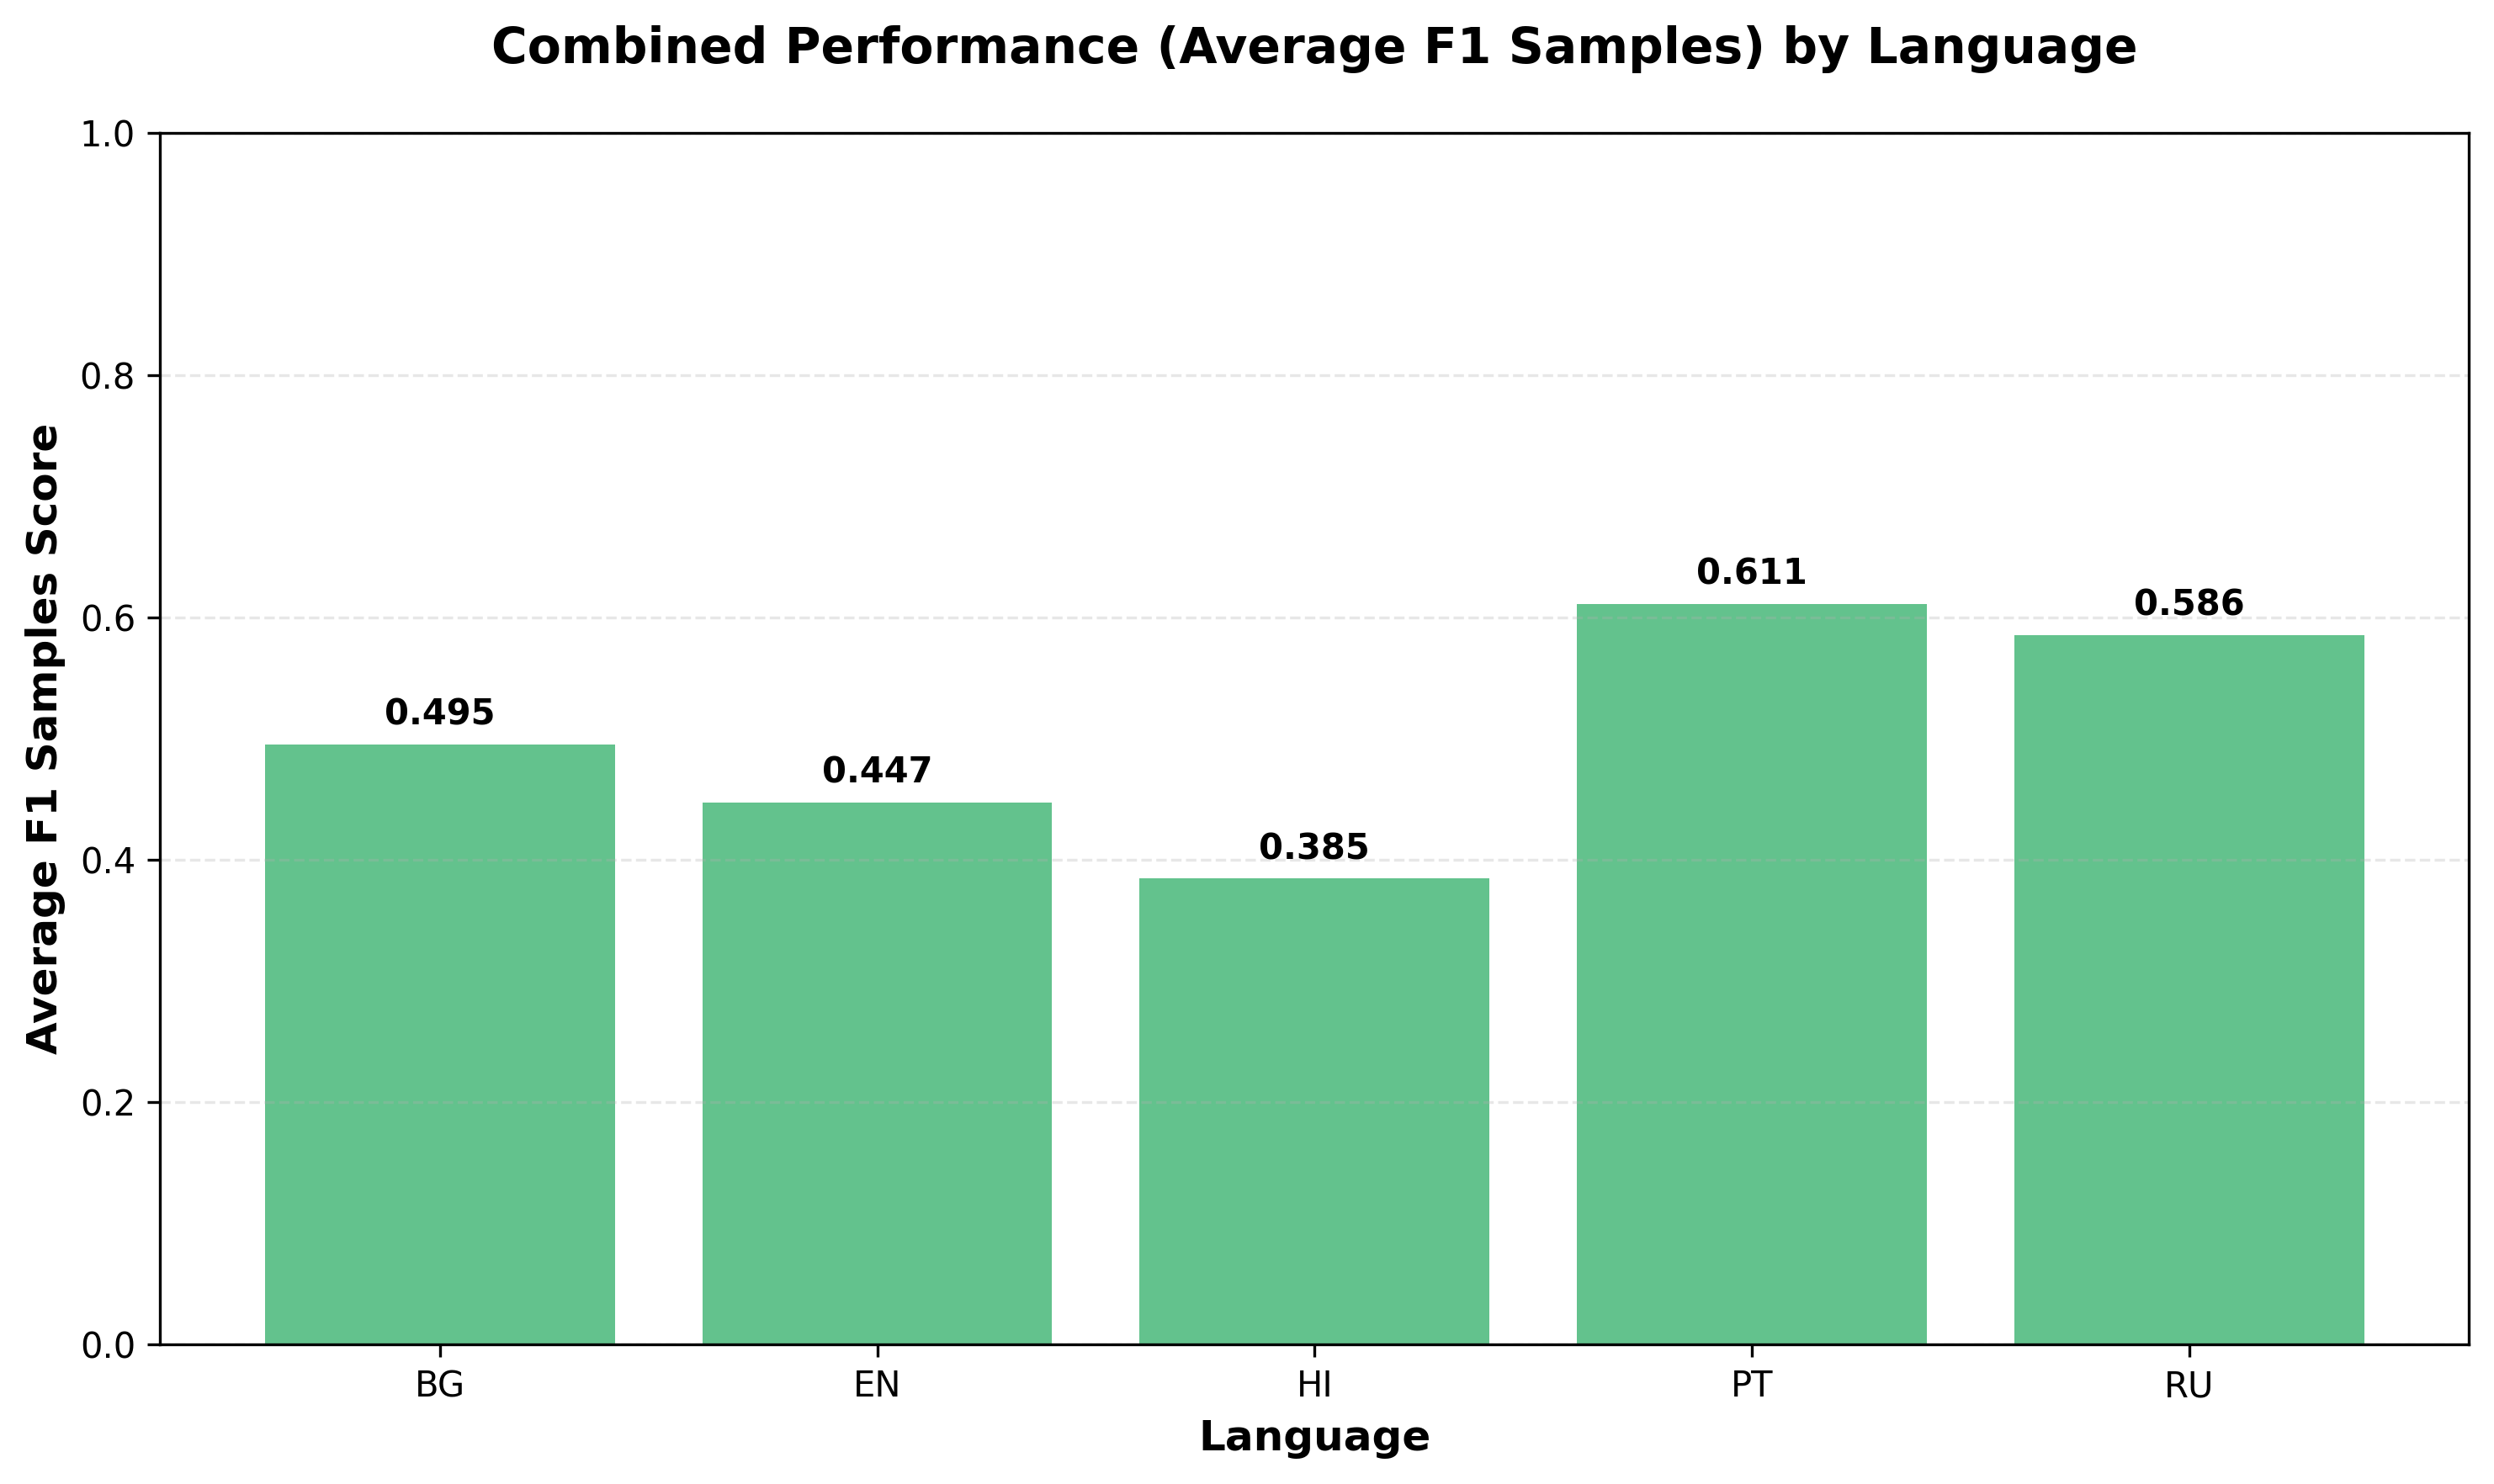
\includegraphics[width=0.85\textwidth]{gemini25_flash_devset_evaluation/plots/combined_performance_by_language.png}
    \caption{Combined performance across all languages for the no-validation configuration, showing F1 Coarse (narratives) and F1 Sample (subnarratives) metrics.}
    \label{fig:app-no-val-combined}
\end{figure}

\begin{figure}[H]
    \centering
    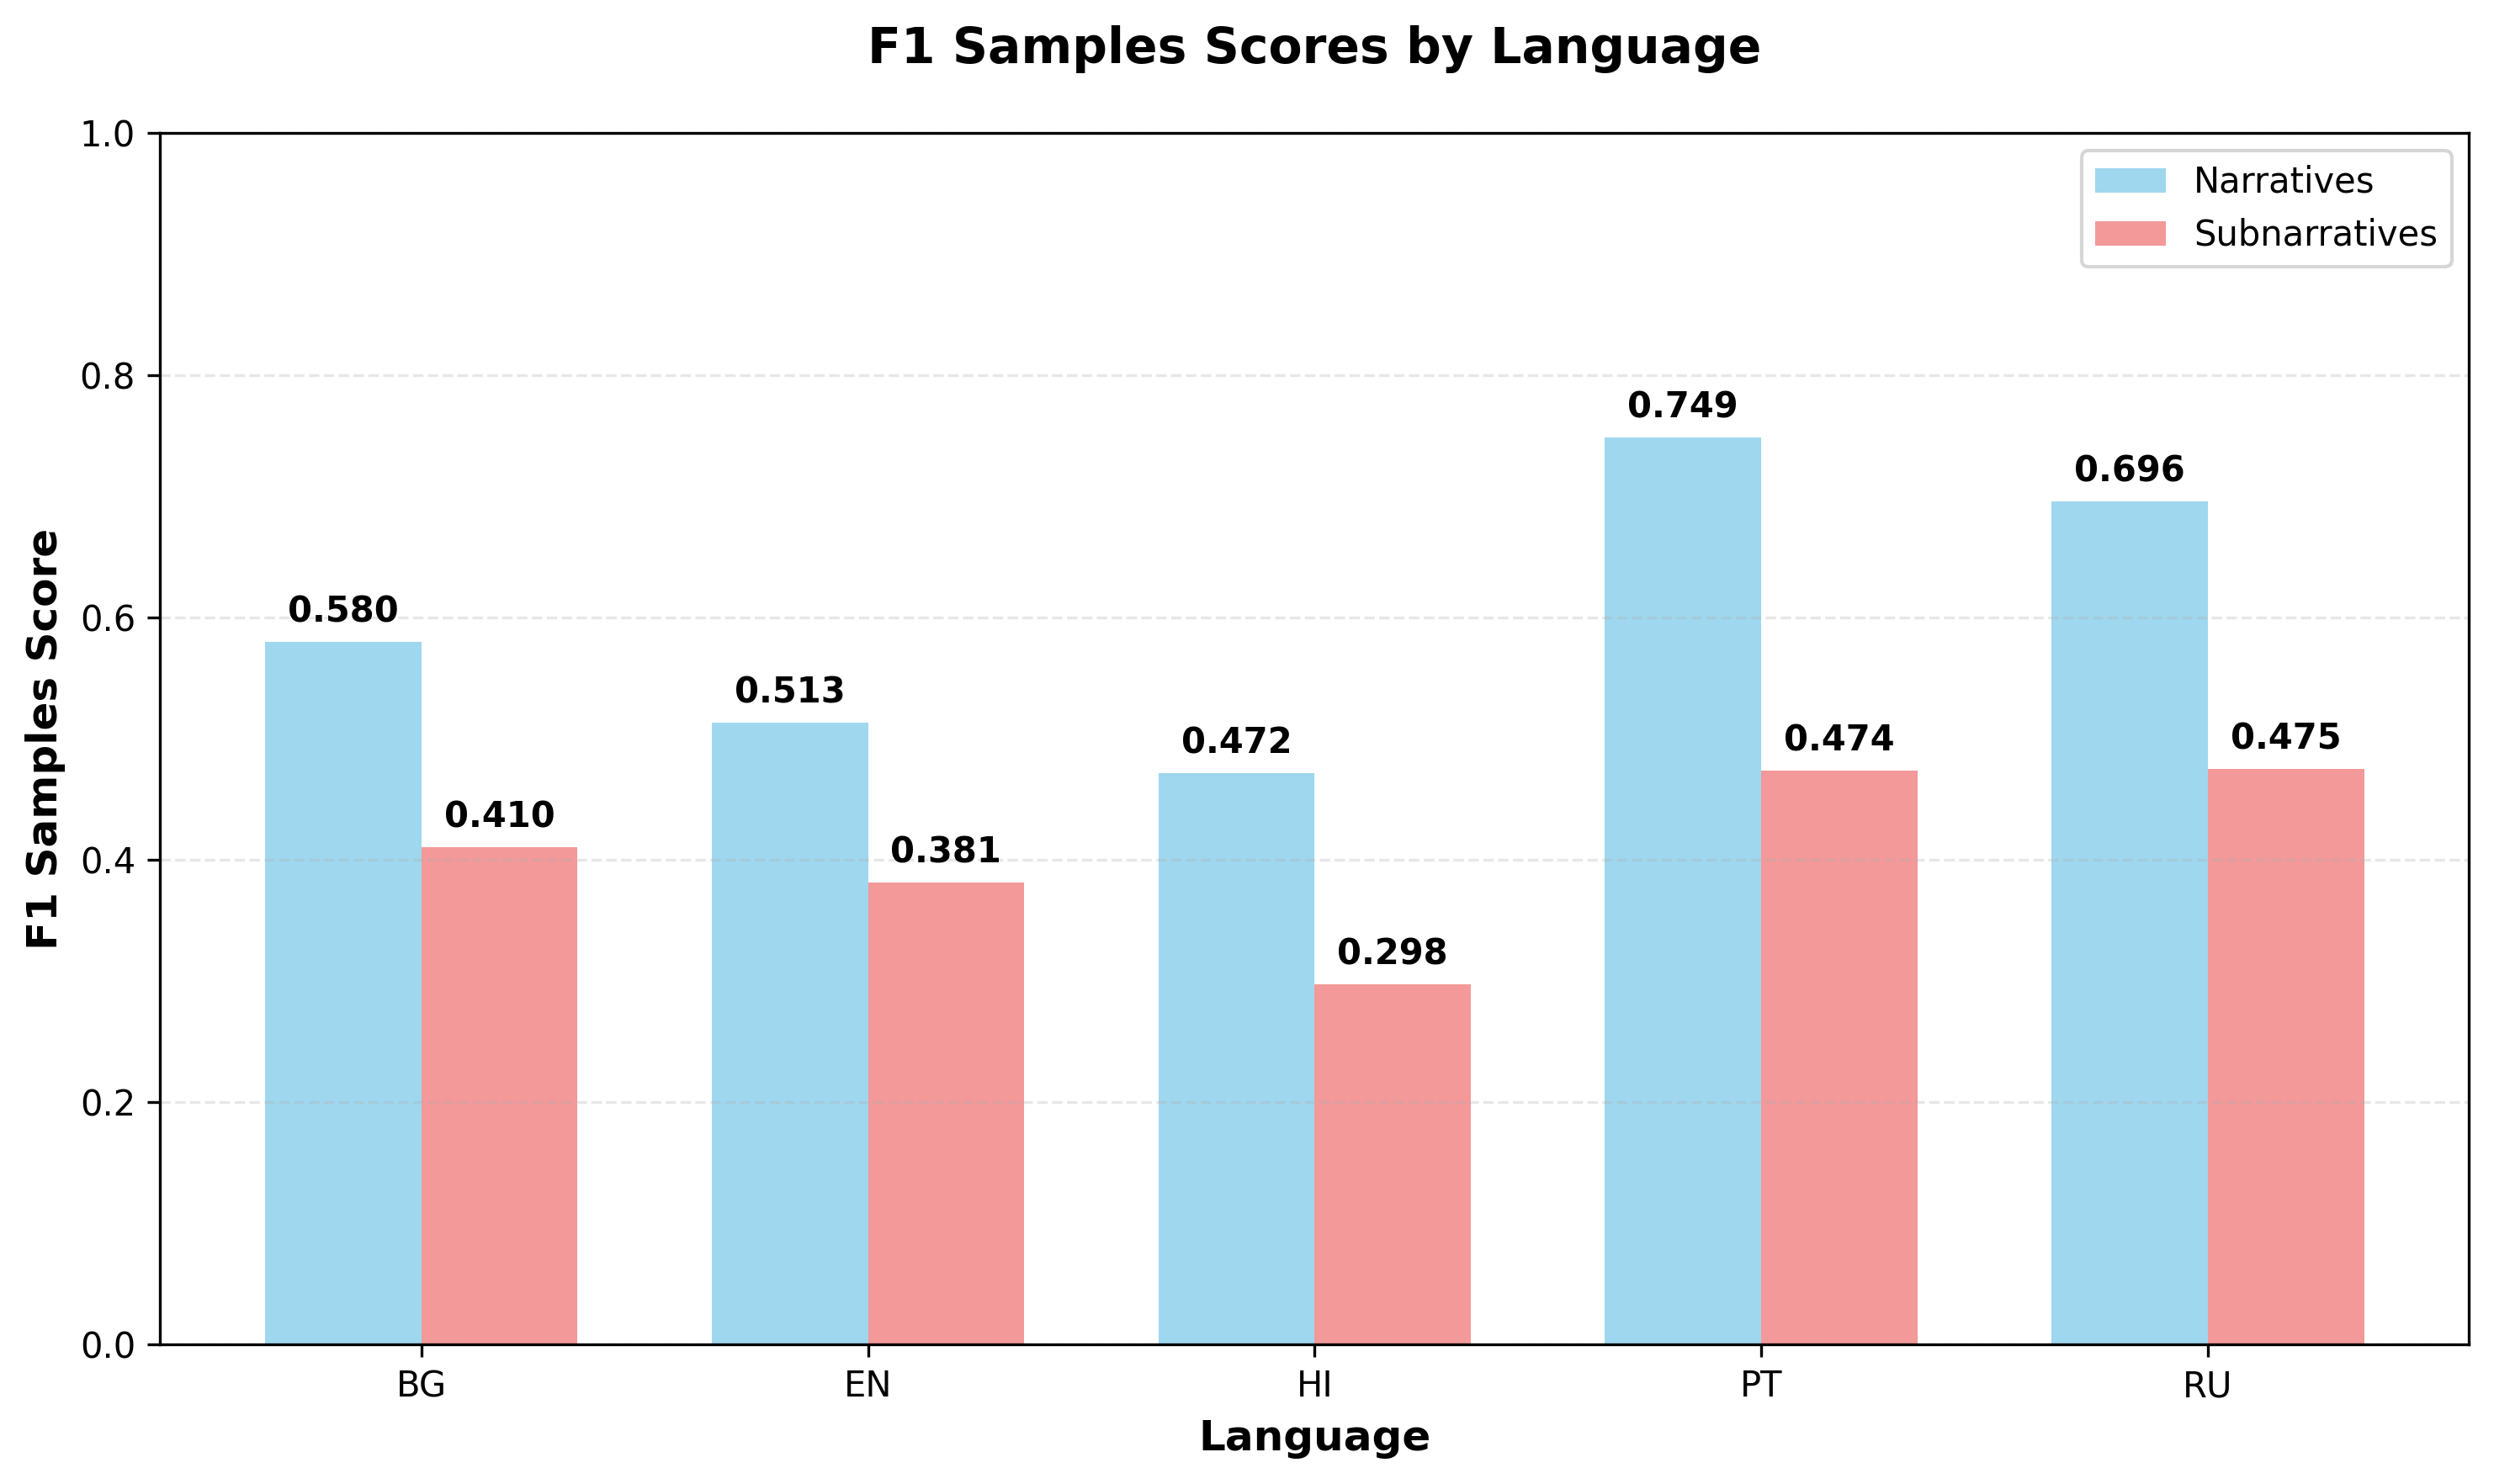
\includegraphics[width=0.85\textwidth]{gemini25_flash_devset_evaluation/plots/f1_samples_by_language.png}
    \caption{F1 Samples performance by language for the no-validation configuration.}
    \label{fig:app-no-val-f1-samples}
\end{figure}

\subsection{Bulgarian (BG) Performance}

\begin{figure}[H]
    \centering
    \begin{subfigure}[b]{0.48\textwidth}
        \centering
        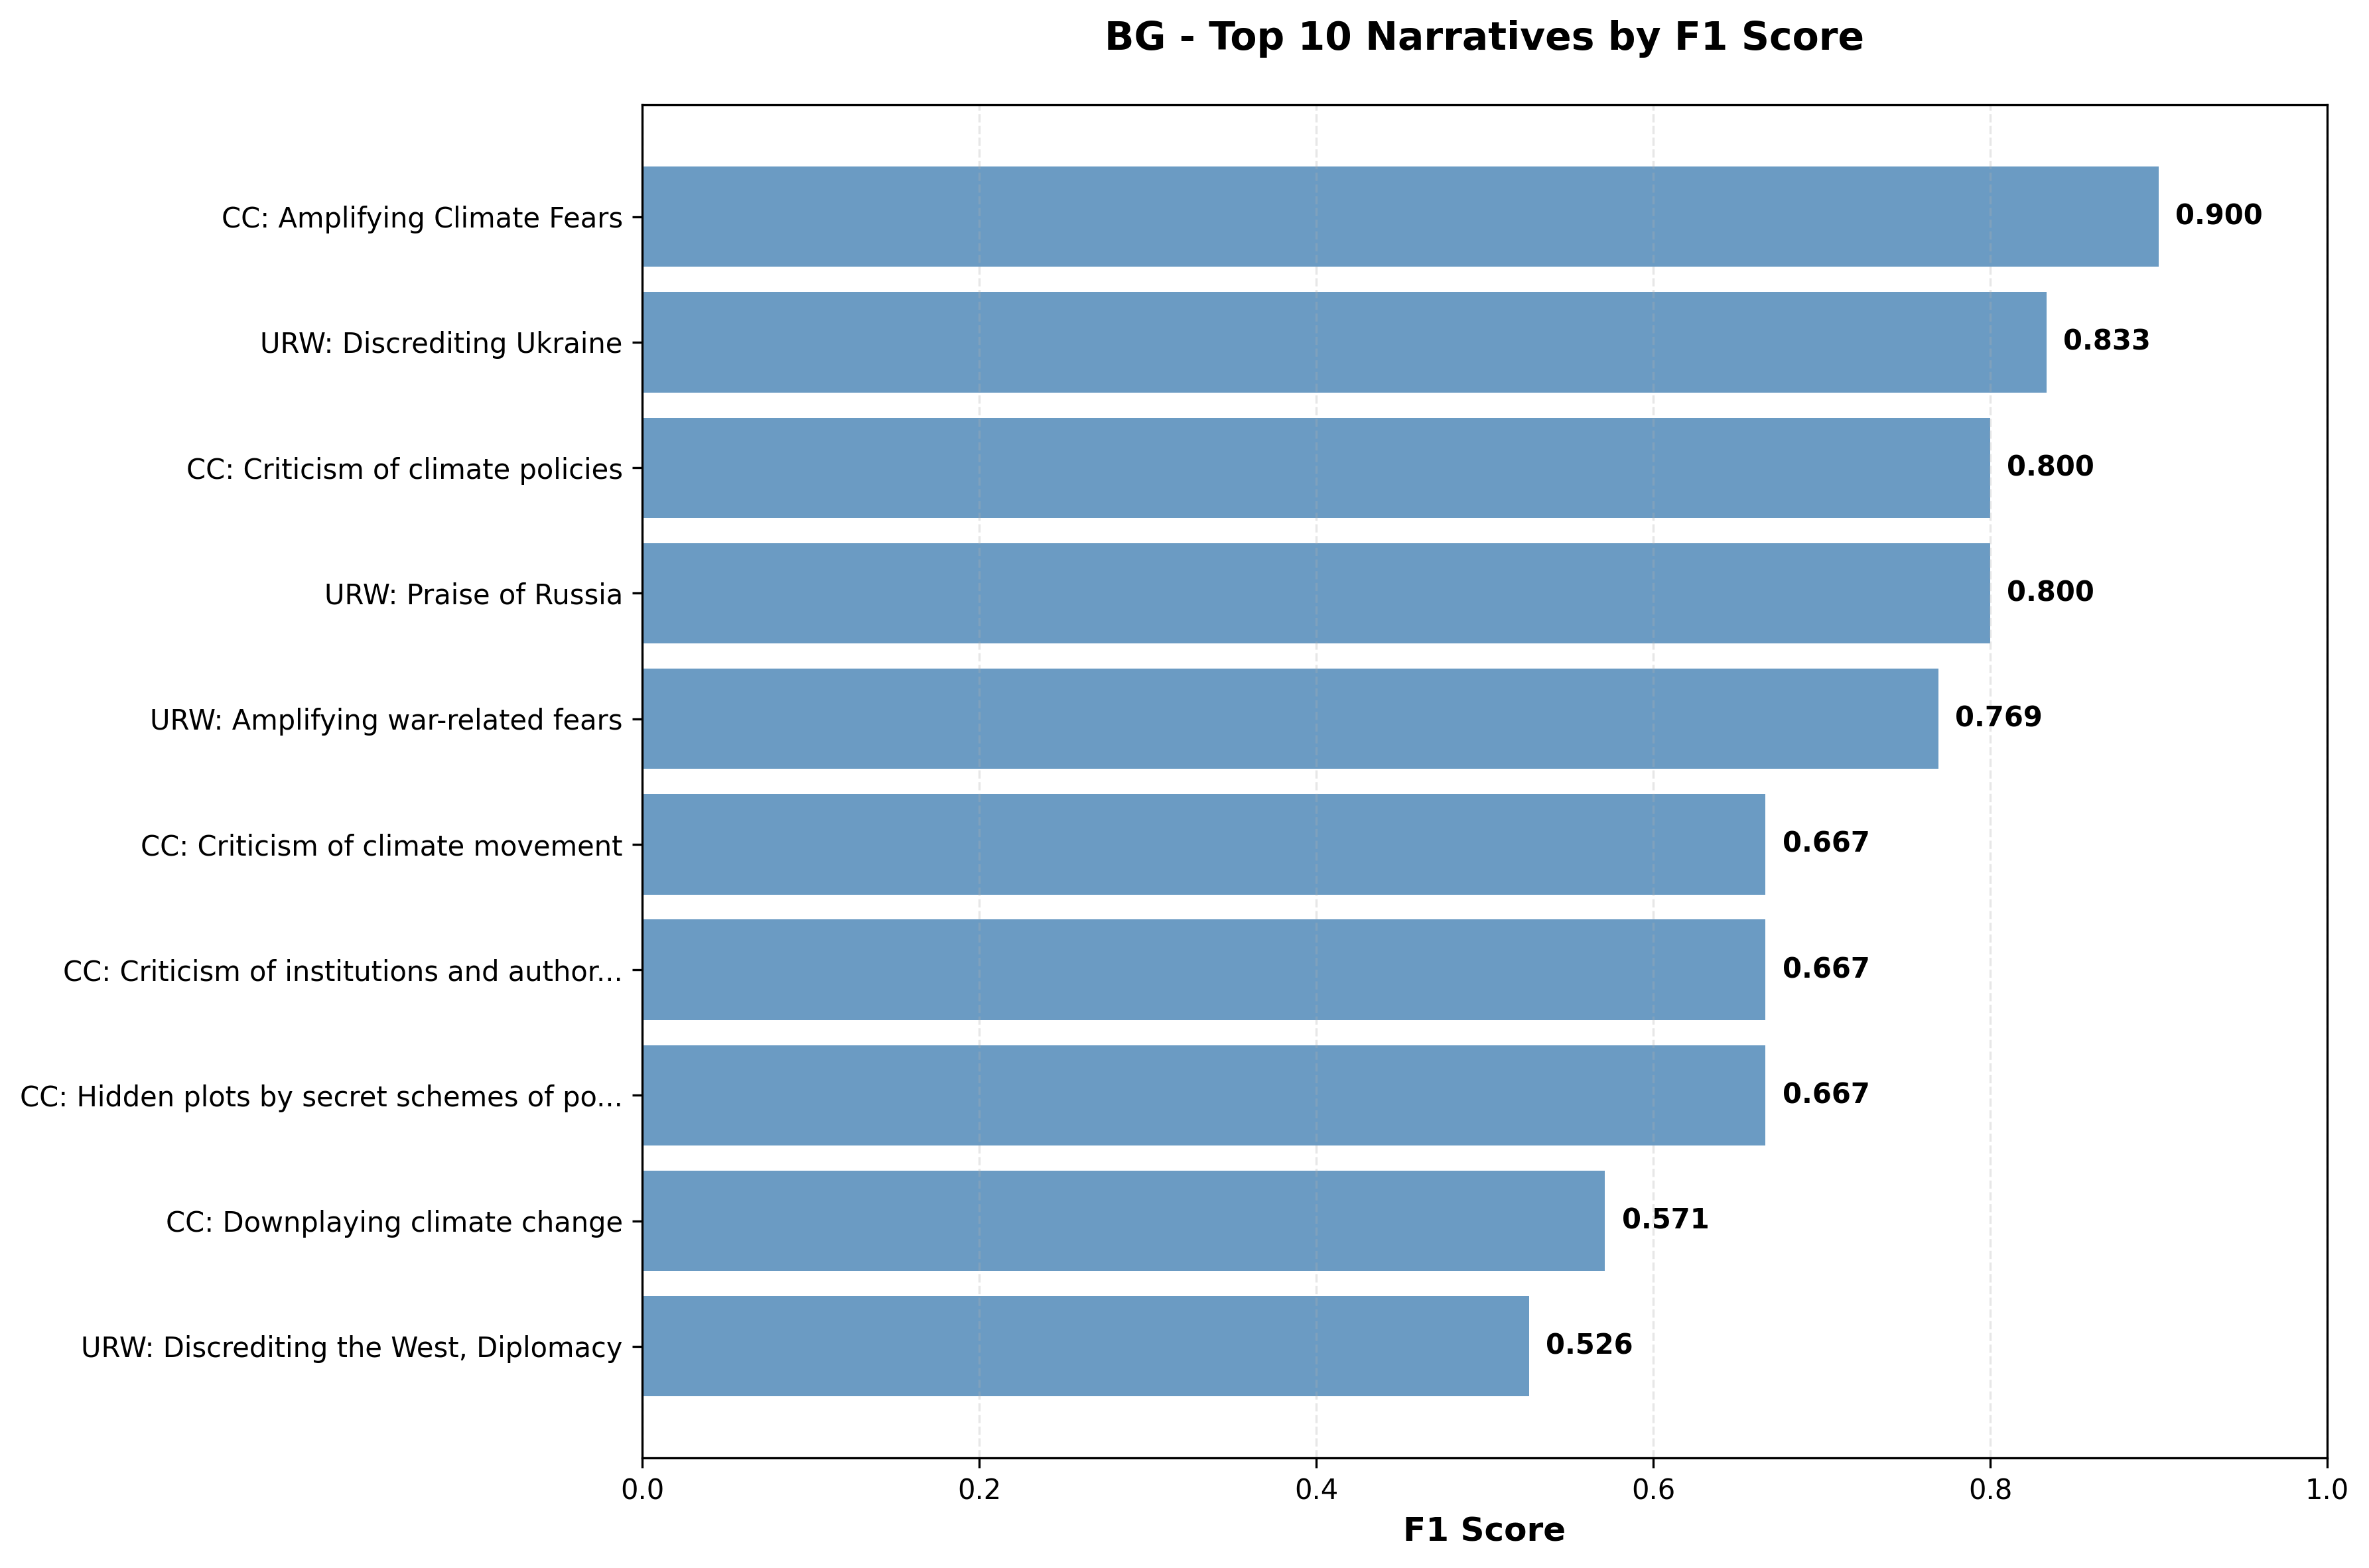
\includegraphics[width=\textwidth]{gemini25_flash_devset_evaluation/plots/BG_top_narratives_f1_scores.png}
        \caption{Top narrative F1 scores}
        \label{fig:app-no-val-bg-narr}
    \end{subfigure}
    \hfill
    \begin{subfigure}[b]{0.48\textwidth}
        \centering
        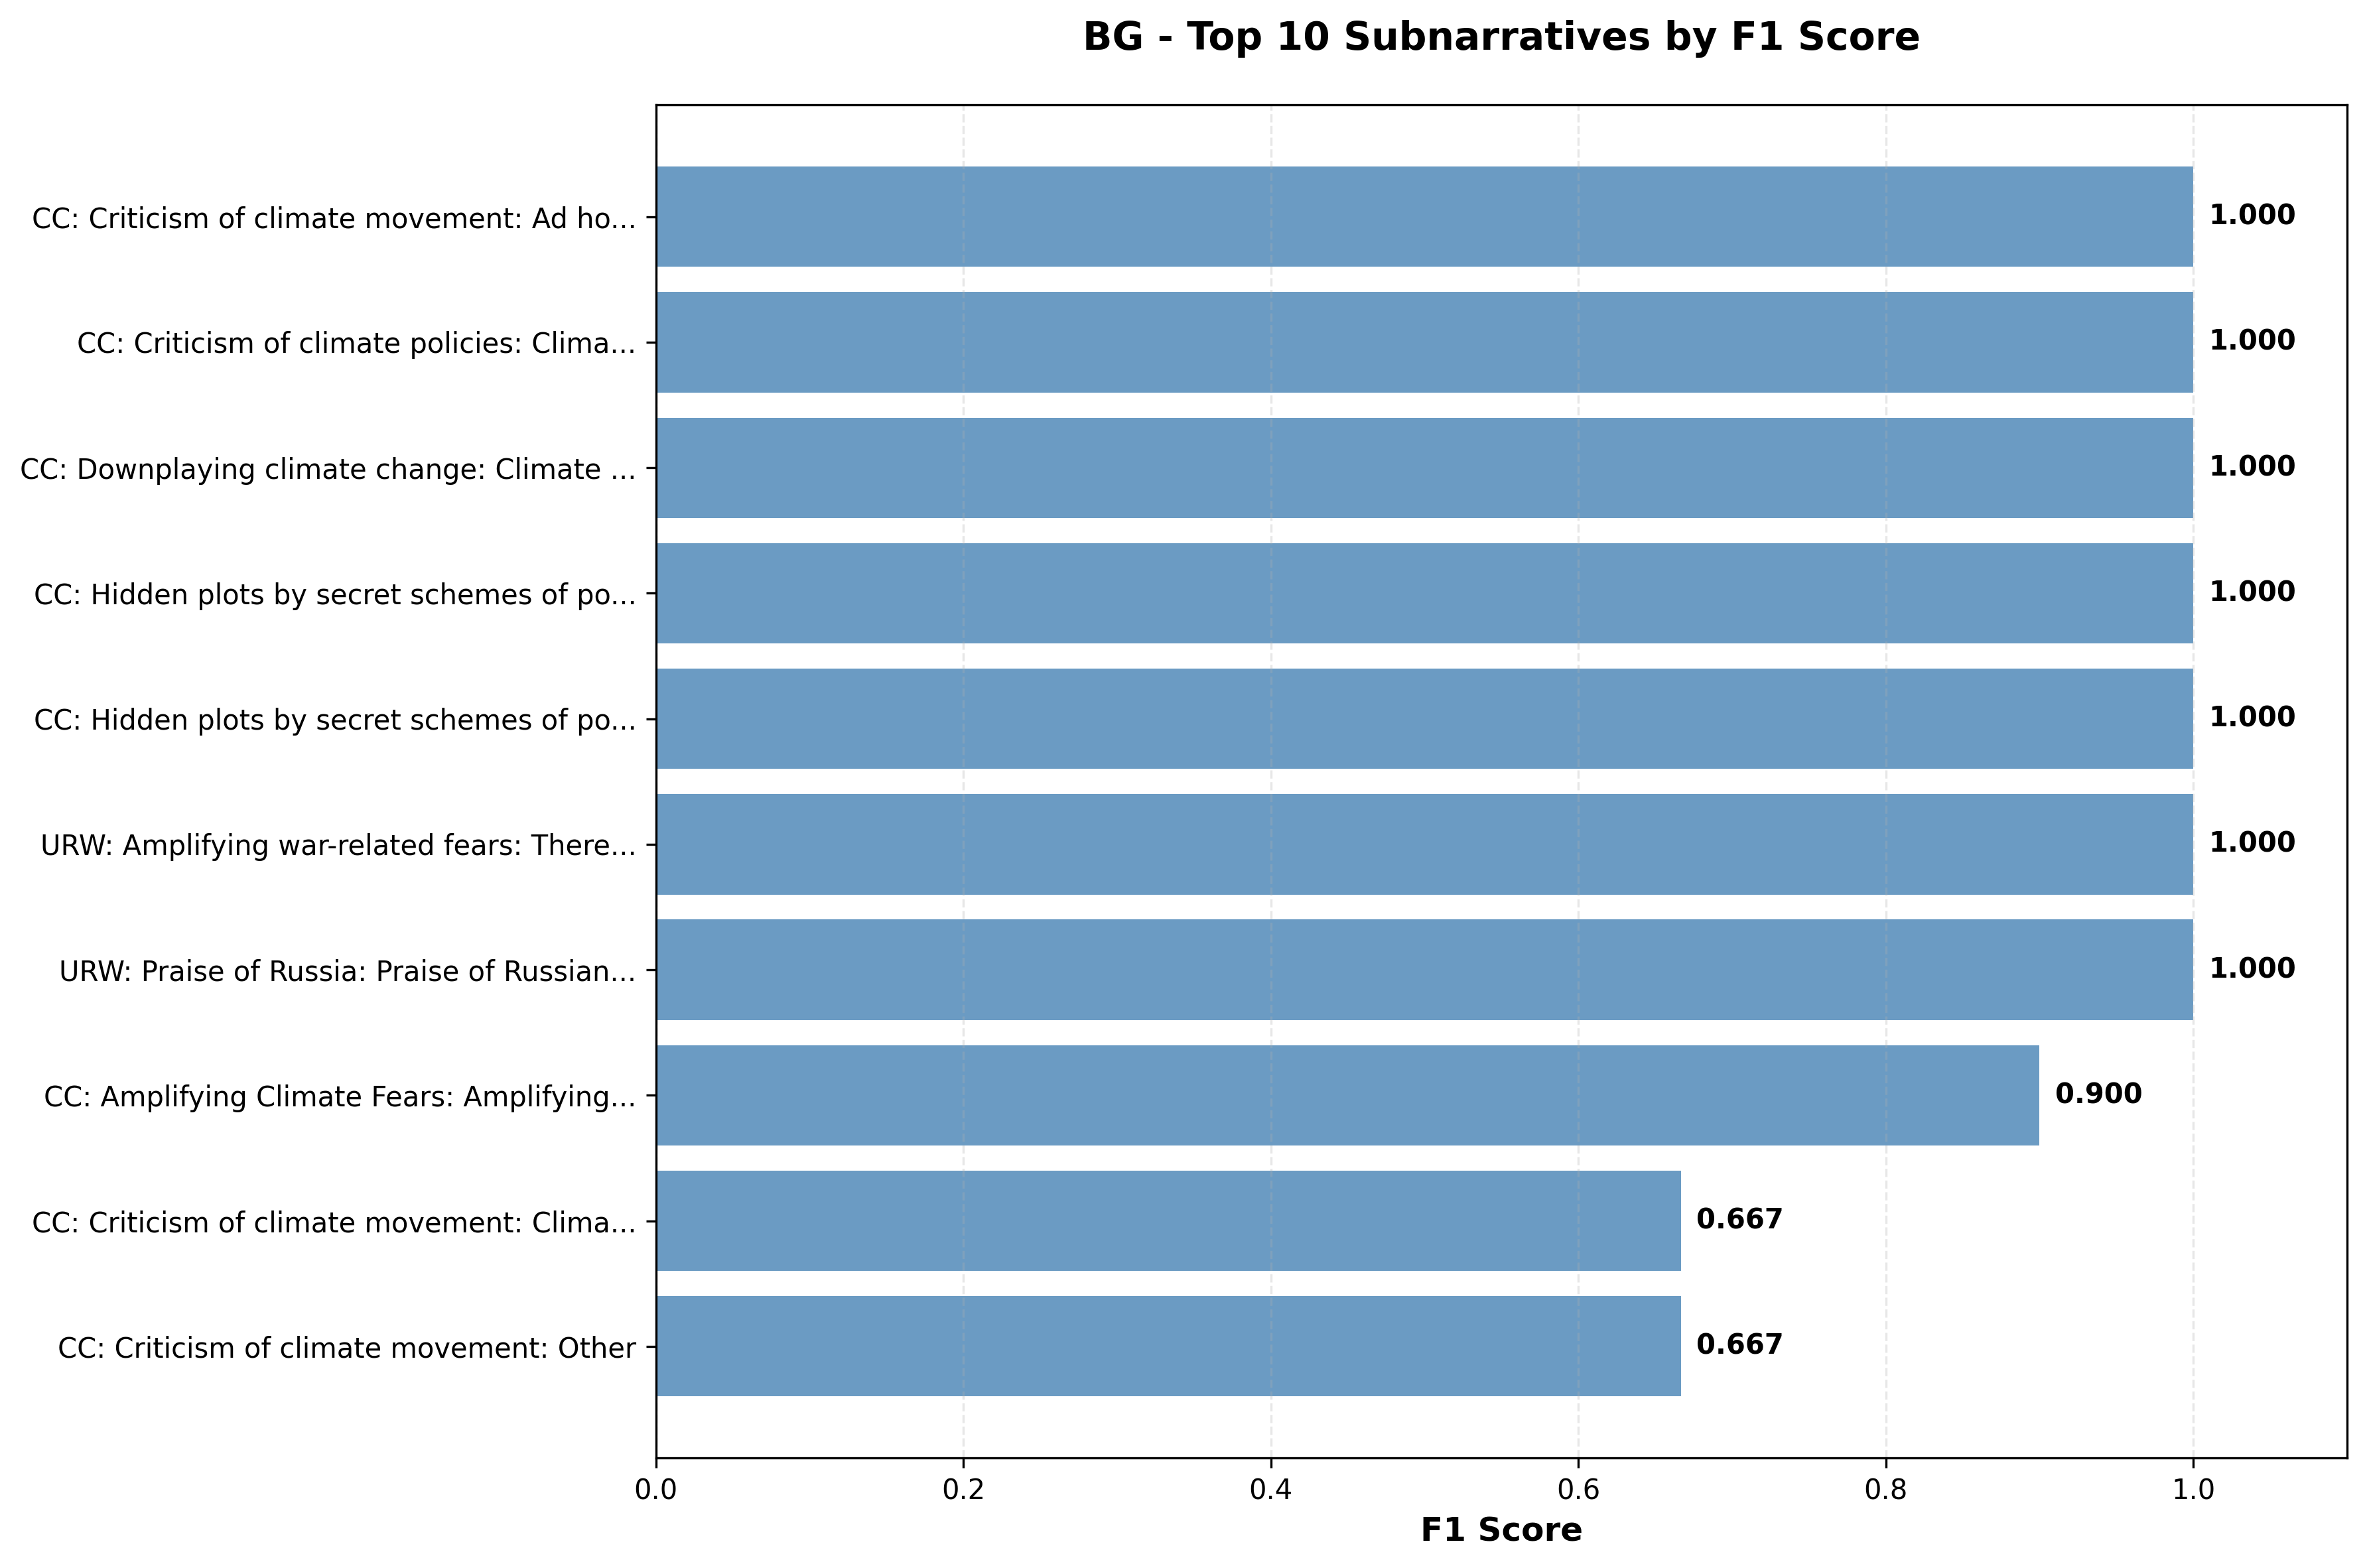
\includegraphics[width=\textwidth]{gemini25_flash_devset_evaluation/plots/BG_top_subnarratives_f1_scores.png}
        \caption{Top subnarrative F1 scores}
        \label{fig:app-no-val-bg-subnarr}
    \end{subfigure}
    \caption{Bulgarian performance breakdown for no-validation configuration.}
    \label{fig:app-no-val-bg}
\end{figure}

\subsection{English (EN) Performance}

\begin{figure}[H]
    \centering
    \begin{subfigure}[b]{0.48\textwidth}
        \centering
        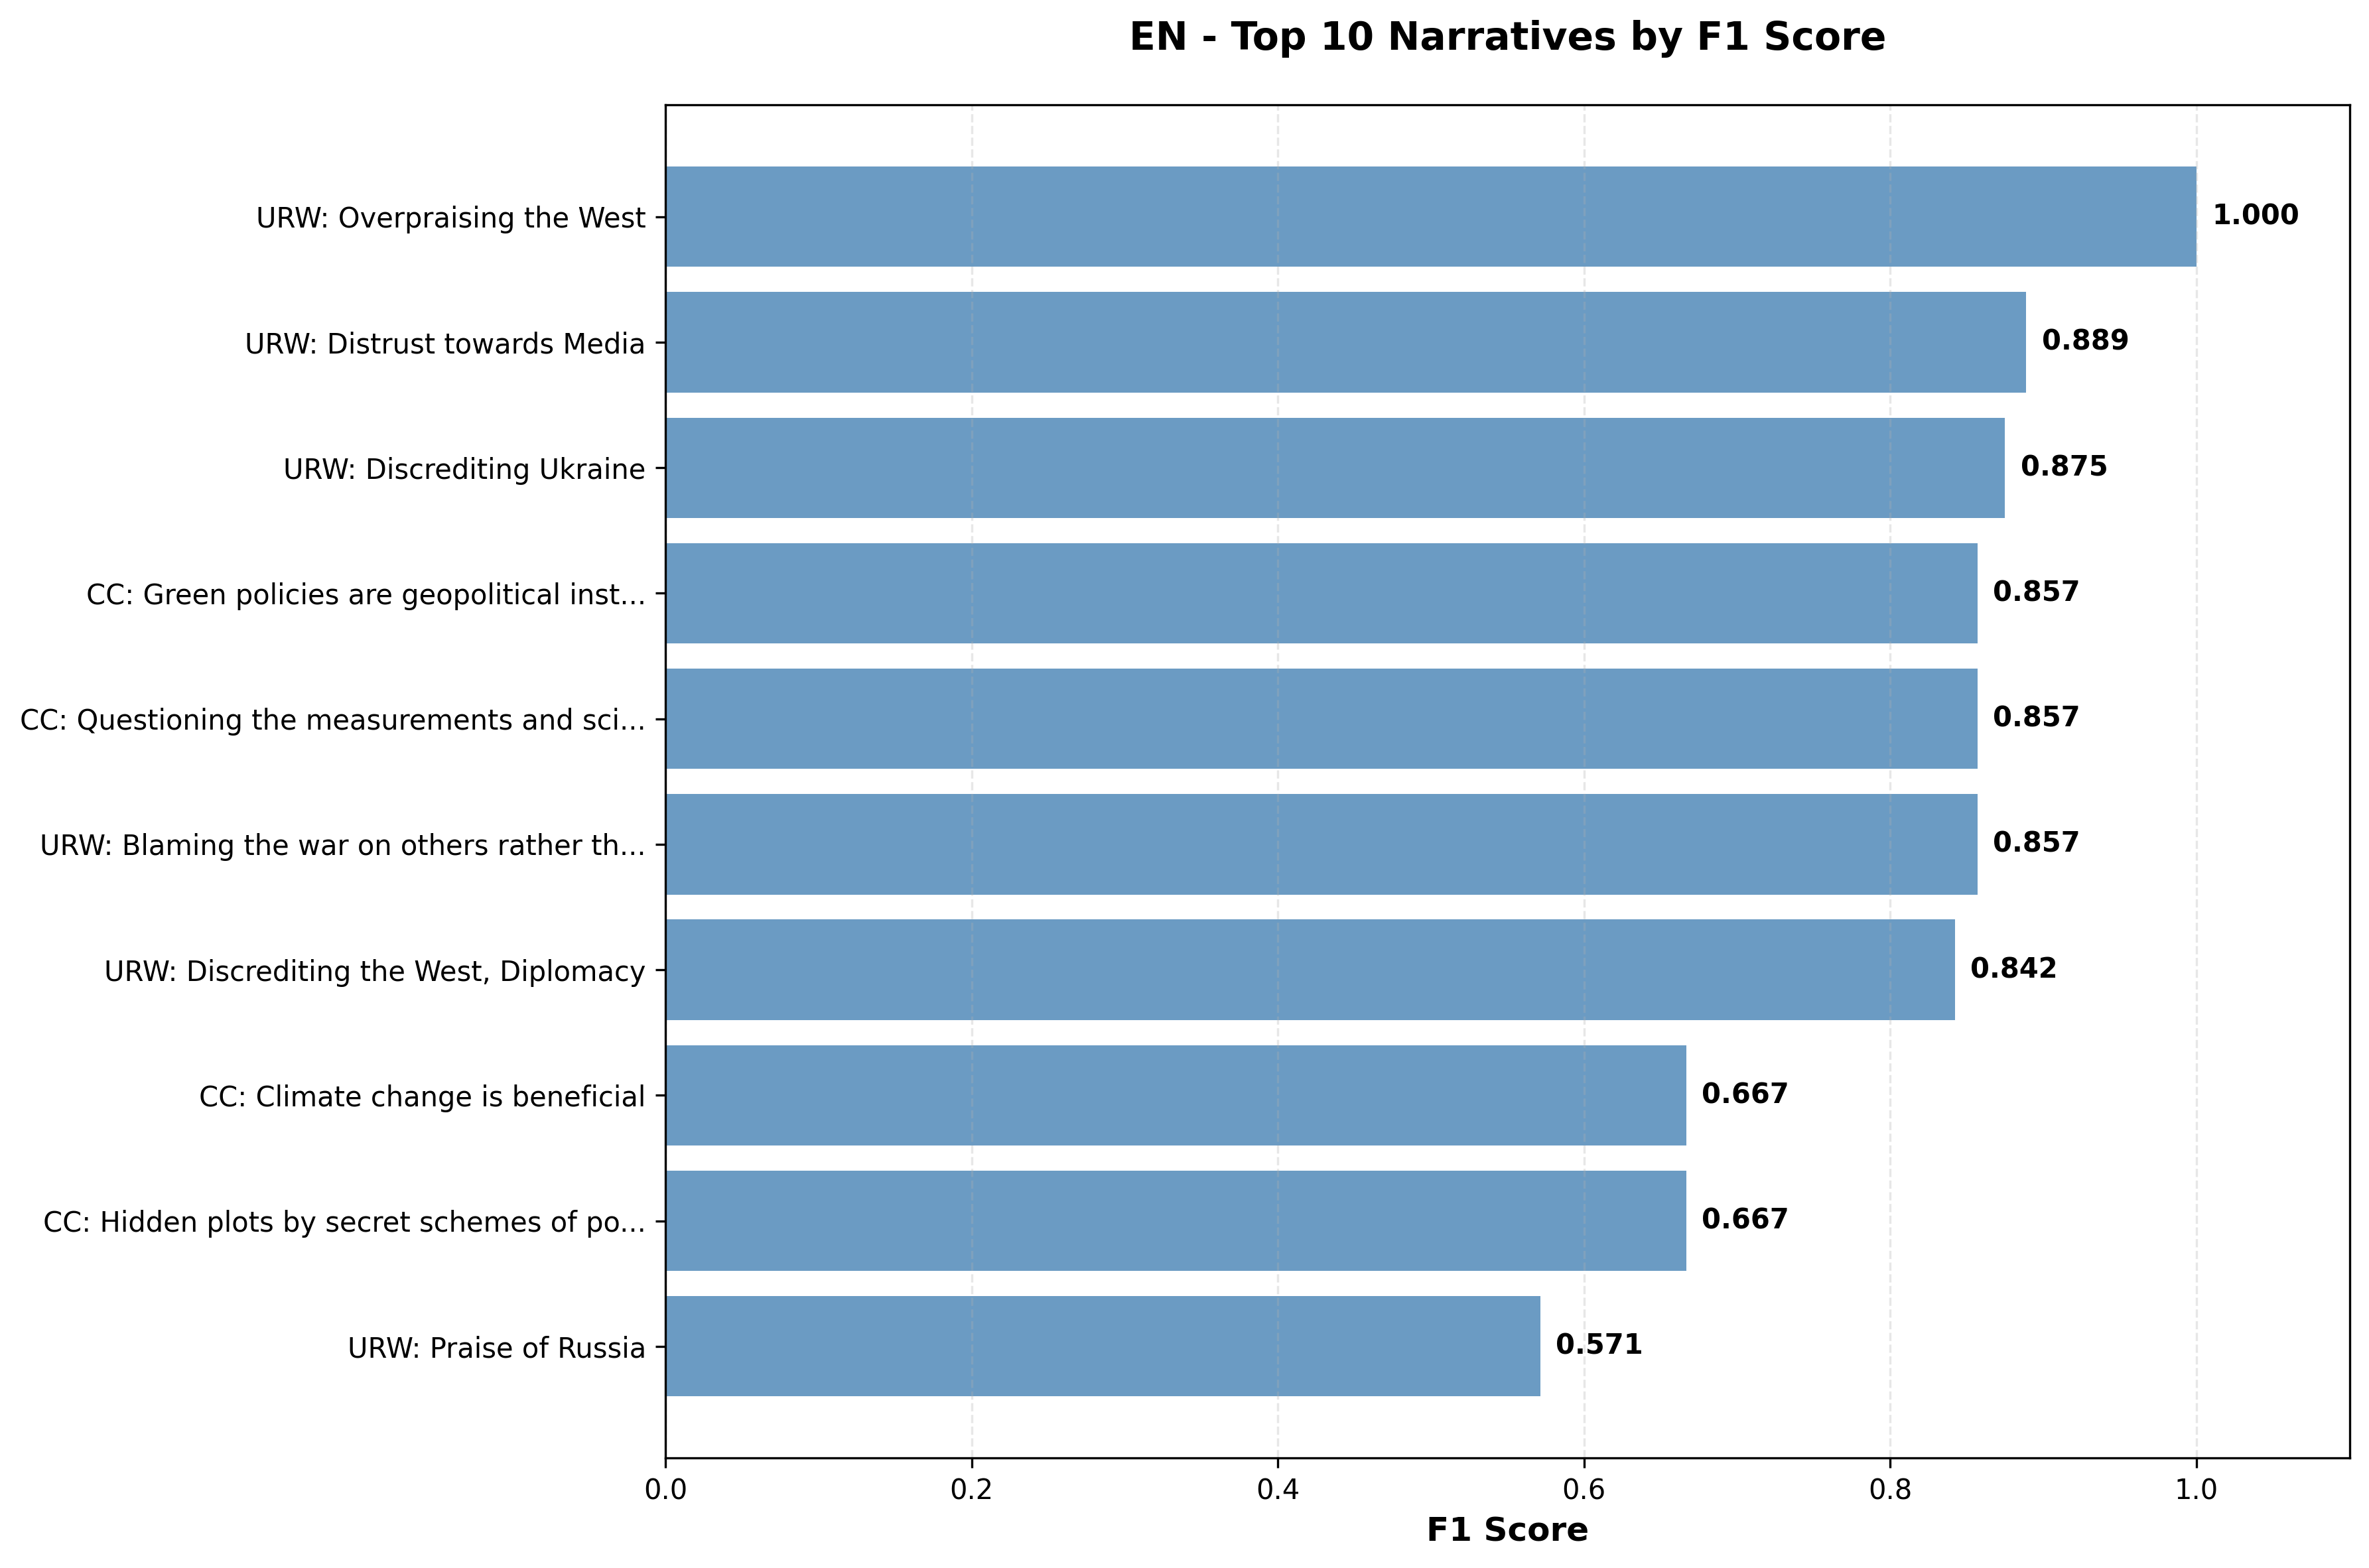
\includegraphics[width=\textwidth]{gemini25_flash_devset_evaluation/plots/EN_top_narratives_f1_scores.png}
        \caption{Top narrative F1 scores}
        \label{fig:app-no-val-en-narr}
    \end{subfigure}
    \hfill
    \begin{subfigure}[b]{0.48\textwidth}
        \centering
        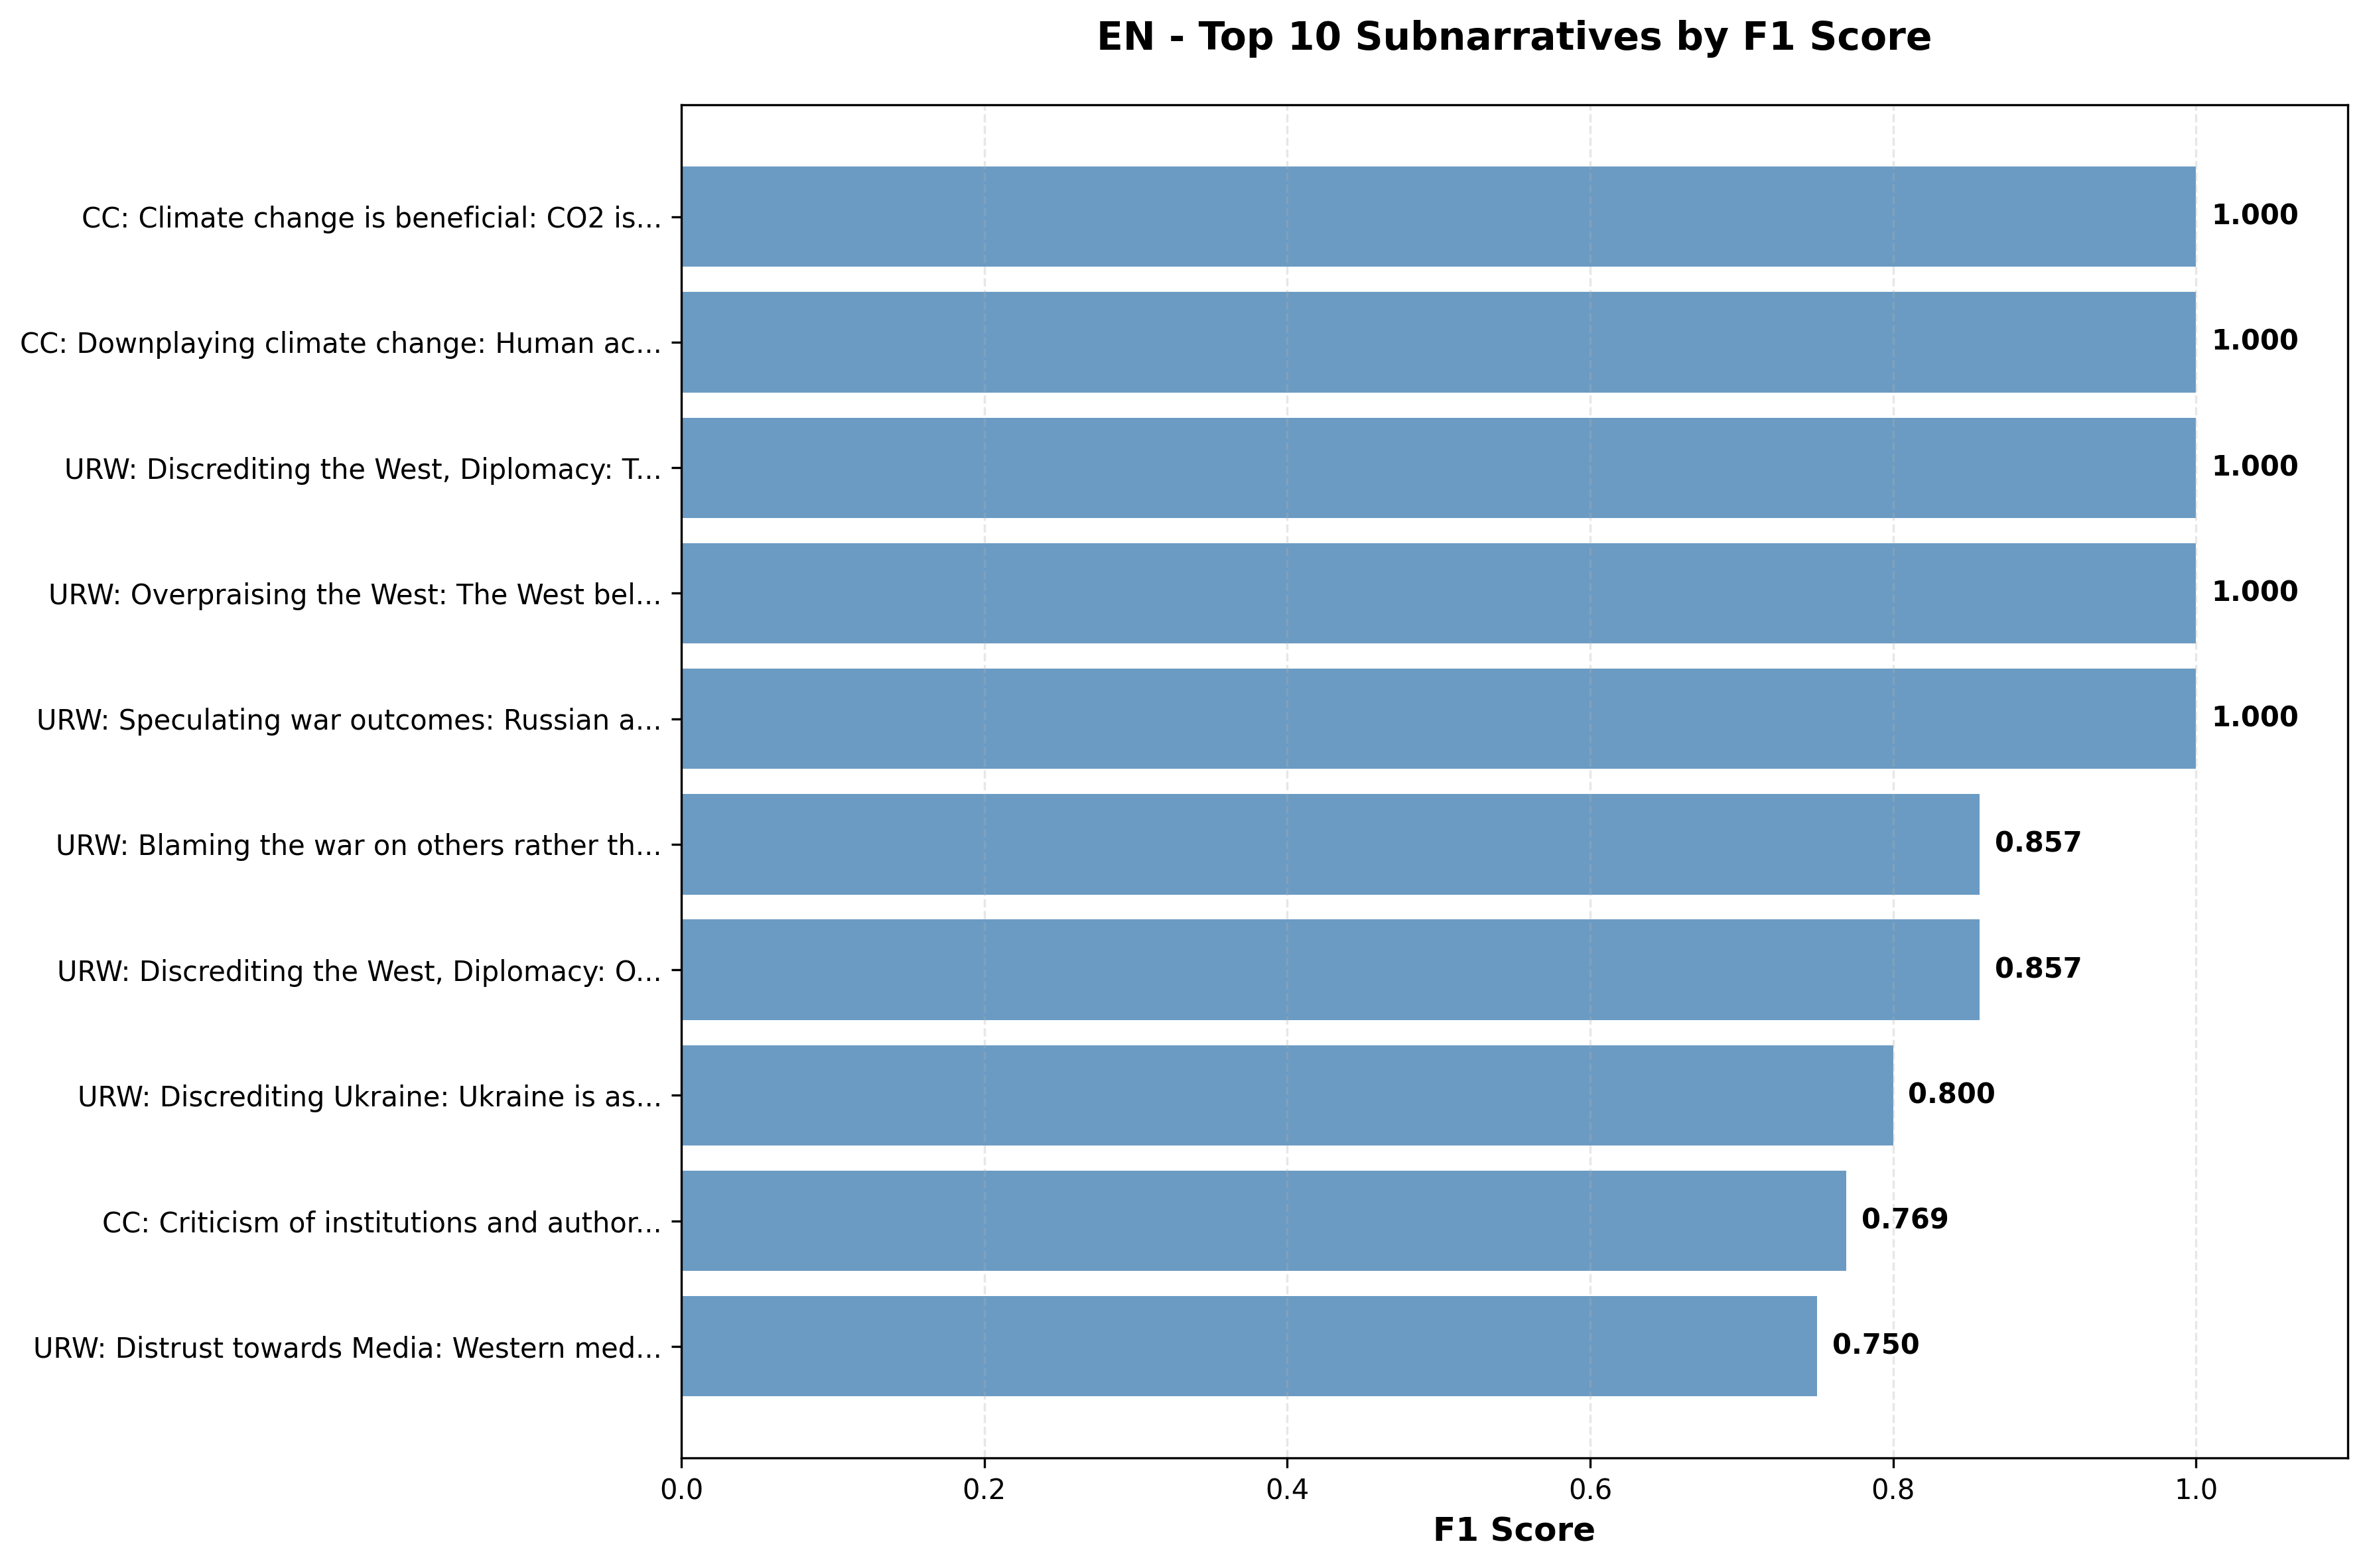
\includegraphics[width=\textwidth]{gemini25_flash_devset_evaluation/plots/EN_top_subnarratives_f1_scores.png}
        \caption{Top subnarrative F1 scores}
        \label{fig:app-no-val-en-subnarr}
    \end{subfigure}
    \caption{English performance breakdown for no-validation configuration.}
    \label{fig:app-no-val-en}
\end{figure}

\subsection{Hindi (HI) Performance}

\begin{figure}[H]
    \centering
    \begin{subfigure}[b]{0.48\textwidth}
        \centering
        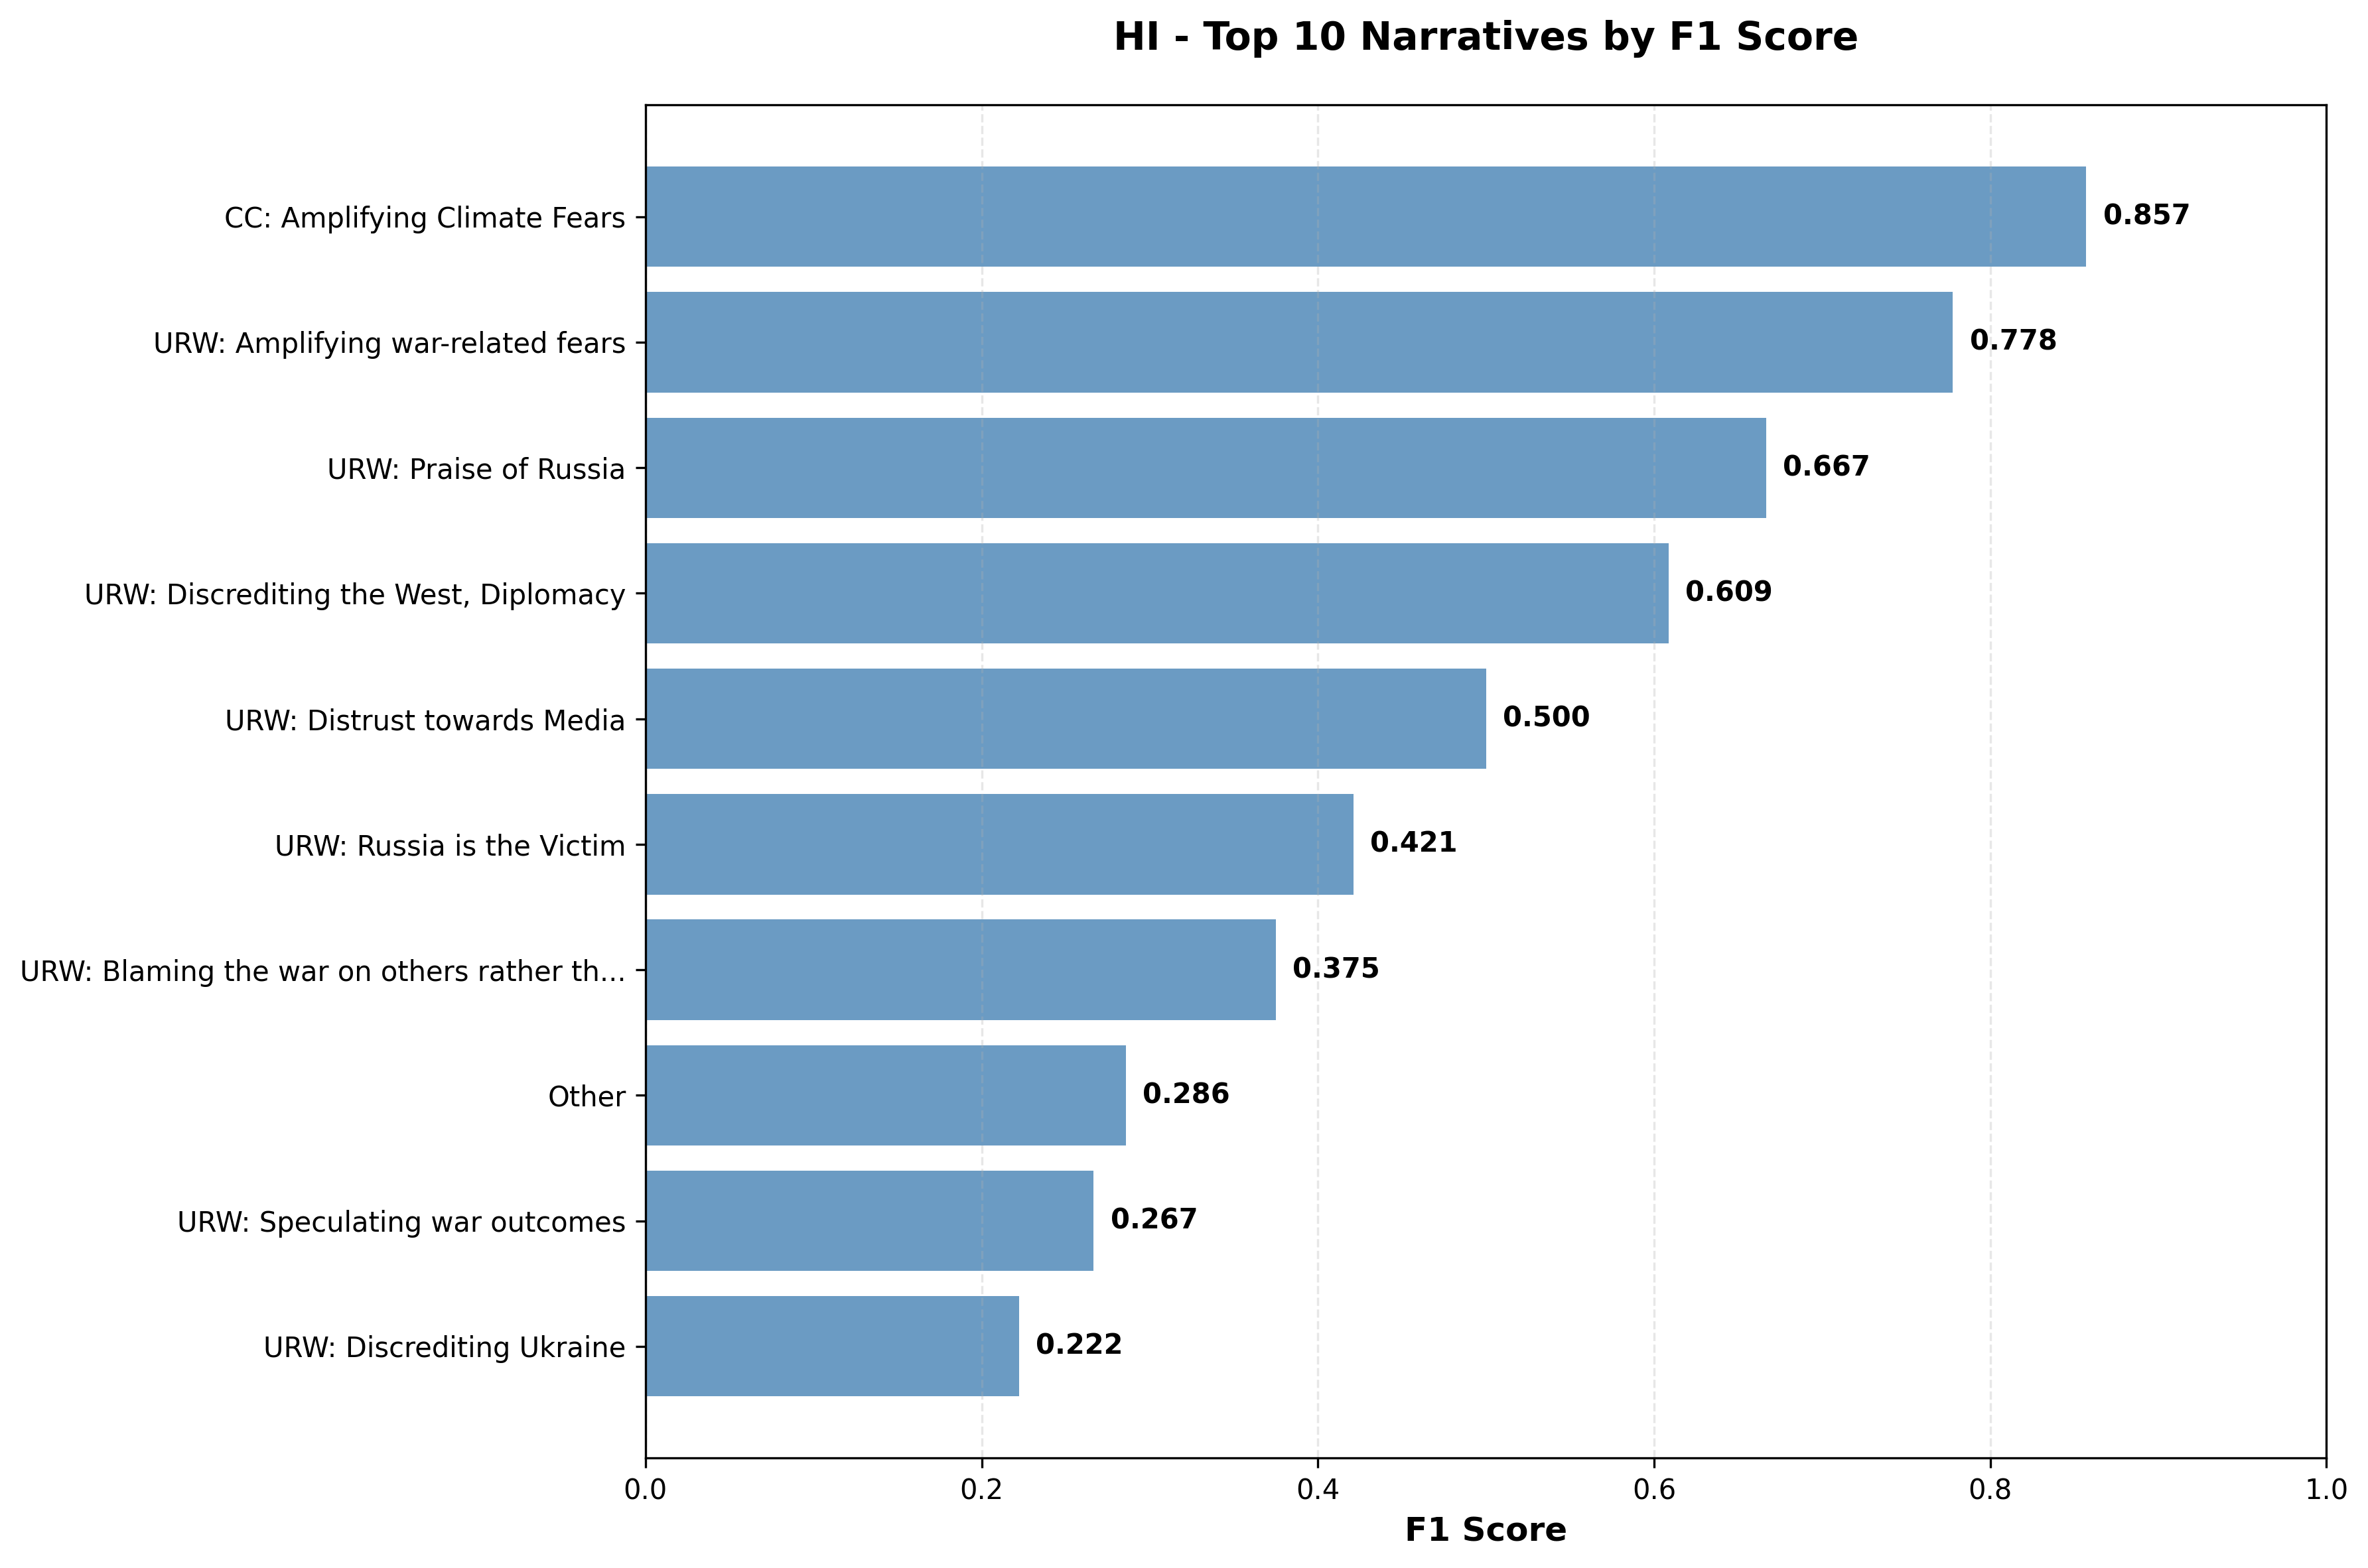
\includegraphics[width=\textwidth]{gemini25_flash_devset_evaluation/plots/HI_top_narratives_f1_scores.png}
        \caption{Top narrative F1 scores}
        \label{fig:app-no-val-hi-narr}
    \end{subfigure}
    \hfill
    \begin{subfigure}[b]{0.48\textwidth}
        \centering
        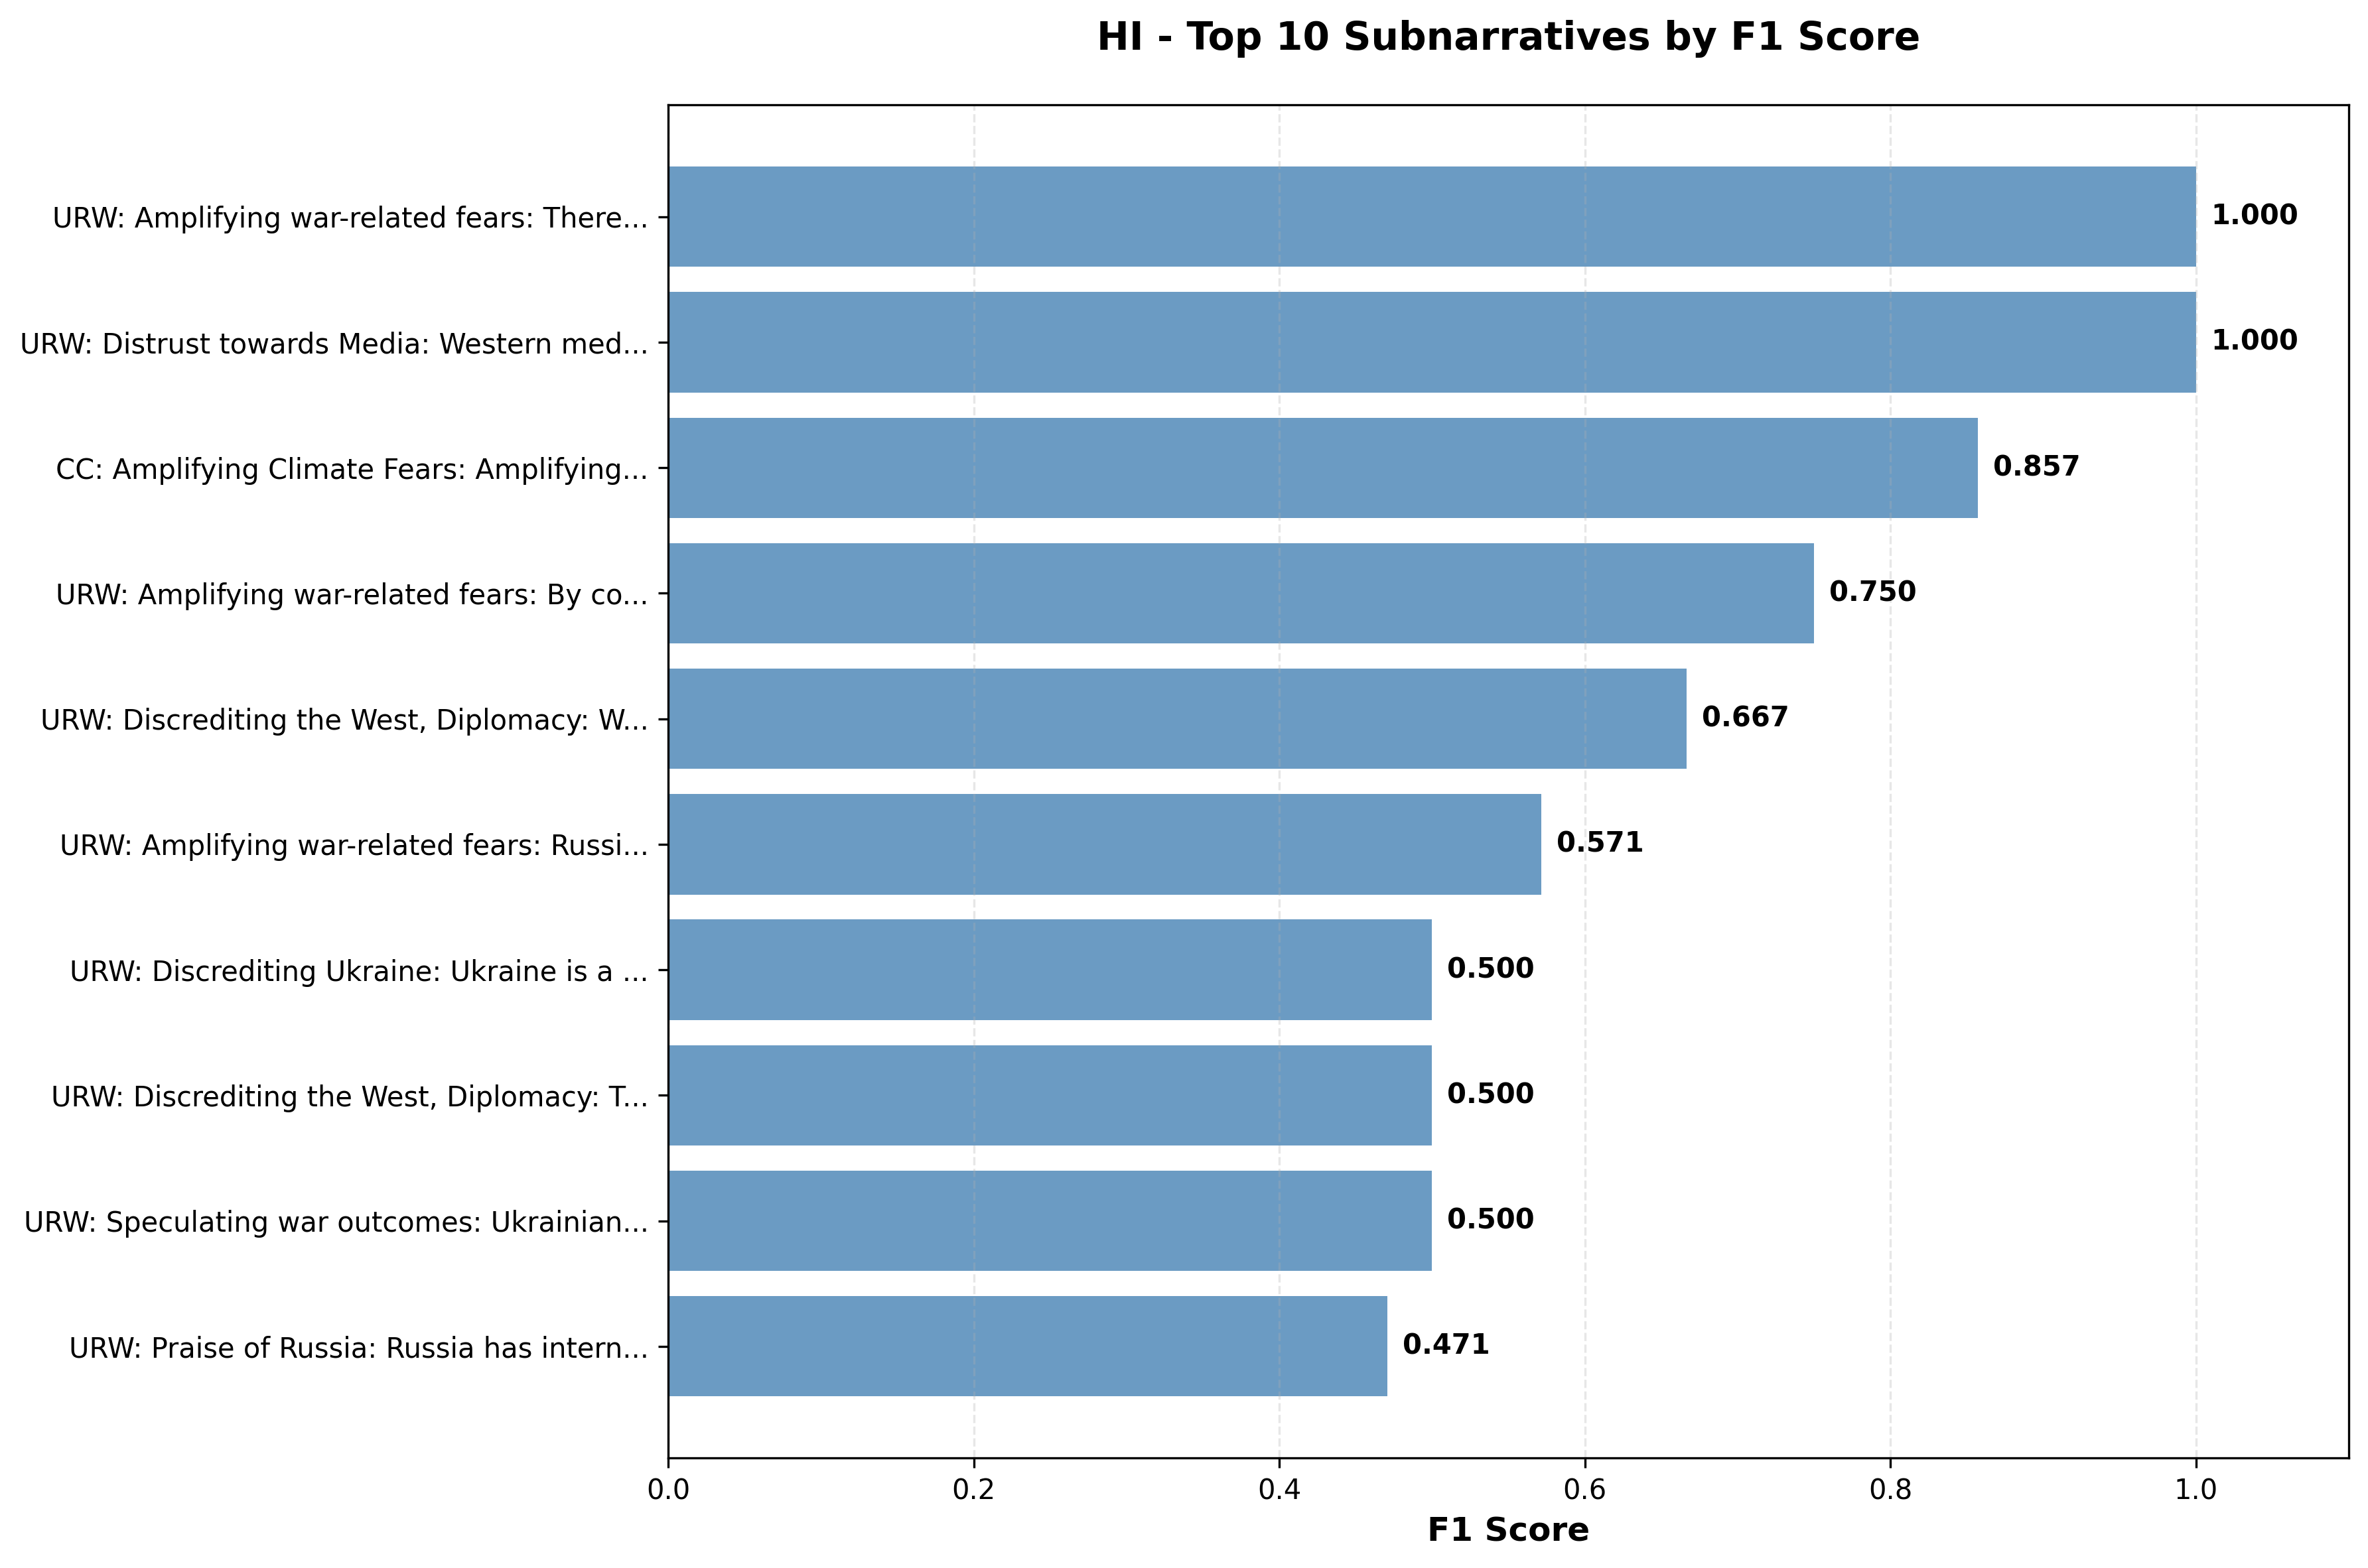
\includegraphics[width=\textwidth]{gemini25_flash_devset_evaluation/plots/HI_top_subnarratives_f1_scores.png}
        \caption{Top subnarrative F1 scores}
        \label{fig:app-no-val-hi-subnarr}
    \end{subfigure}
    \caption{Hindi performance breakdown for no-validation configuration.}
    \label{fig:app-no-val-hi}
\end{figure}

\subsection{Portuguese (PT) Performance}

\begin{figure}[H]
    \centering
    \begin{subfigure}[b]{0.48\textwidth}
        \centering
        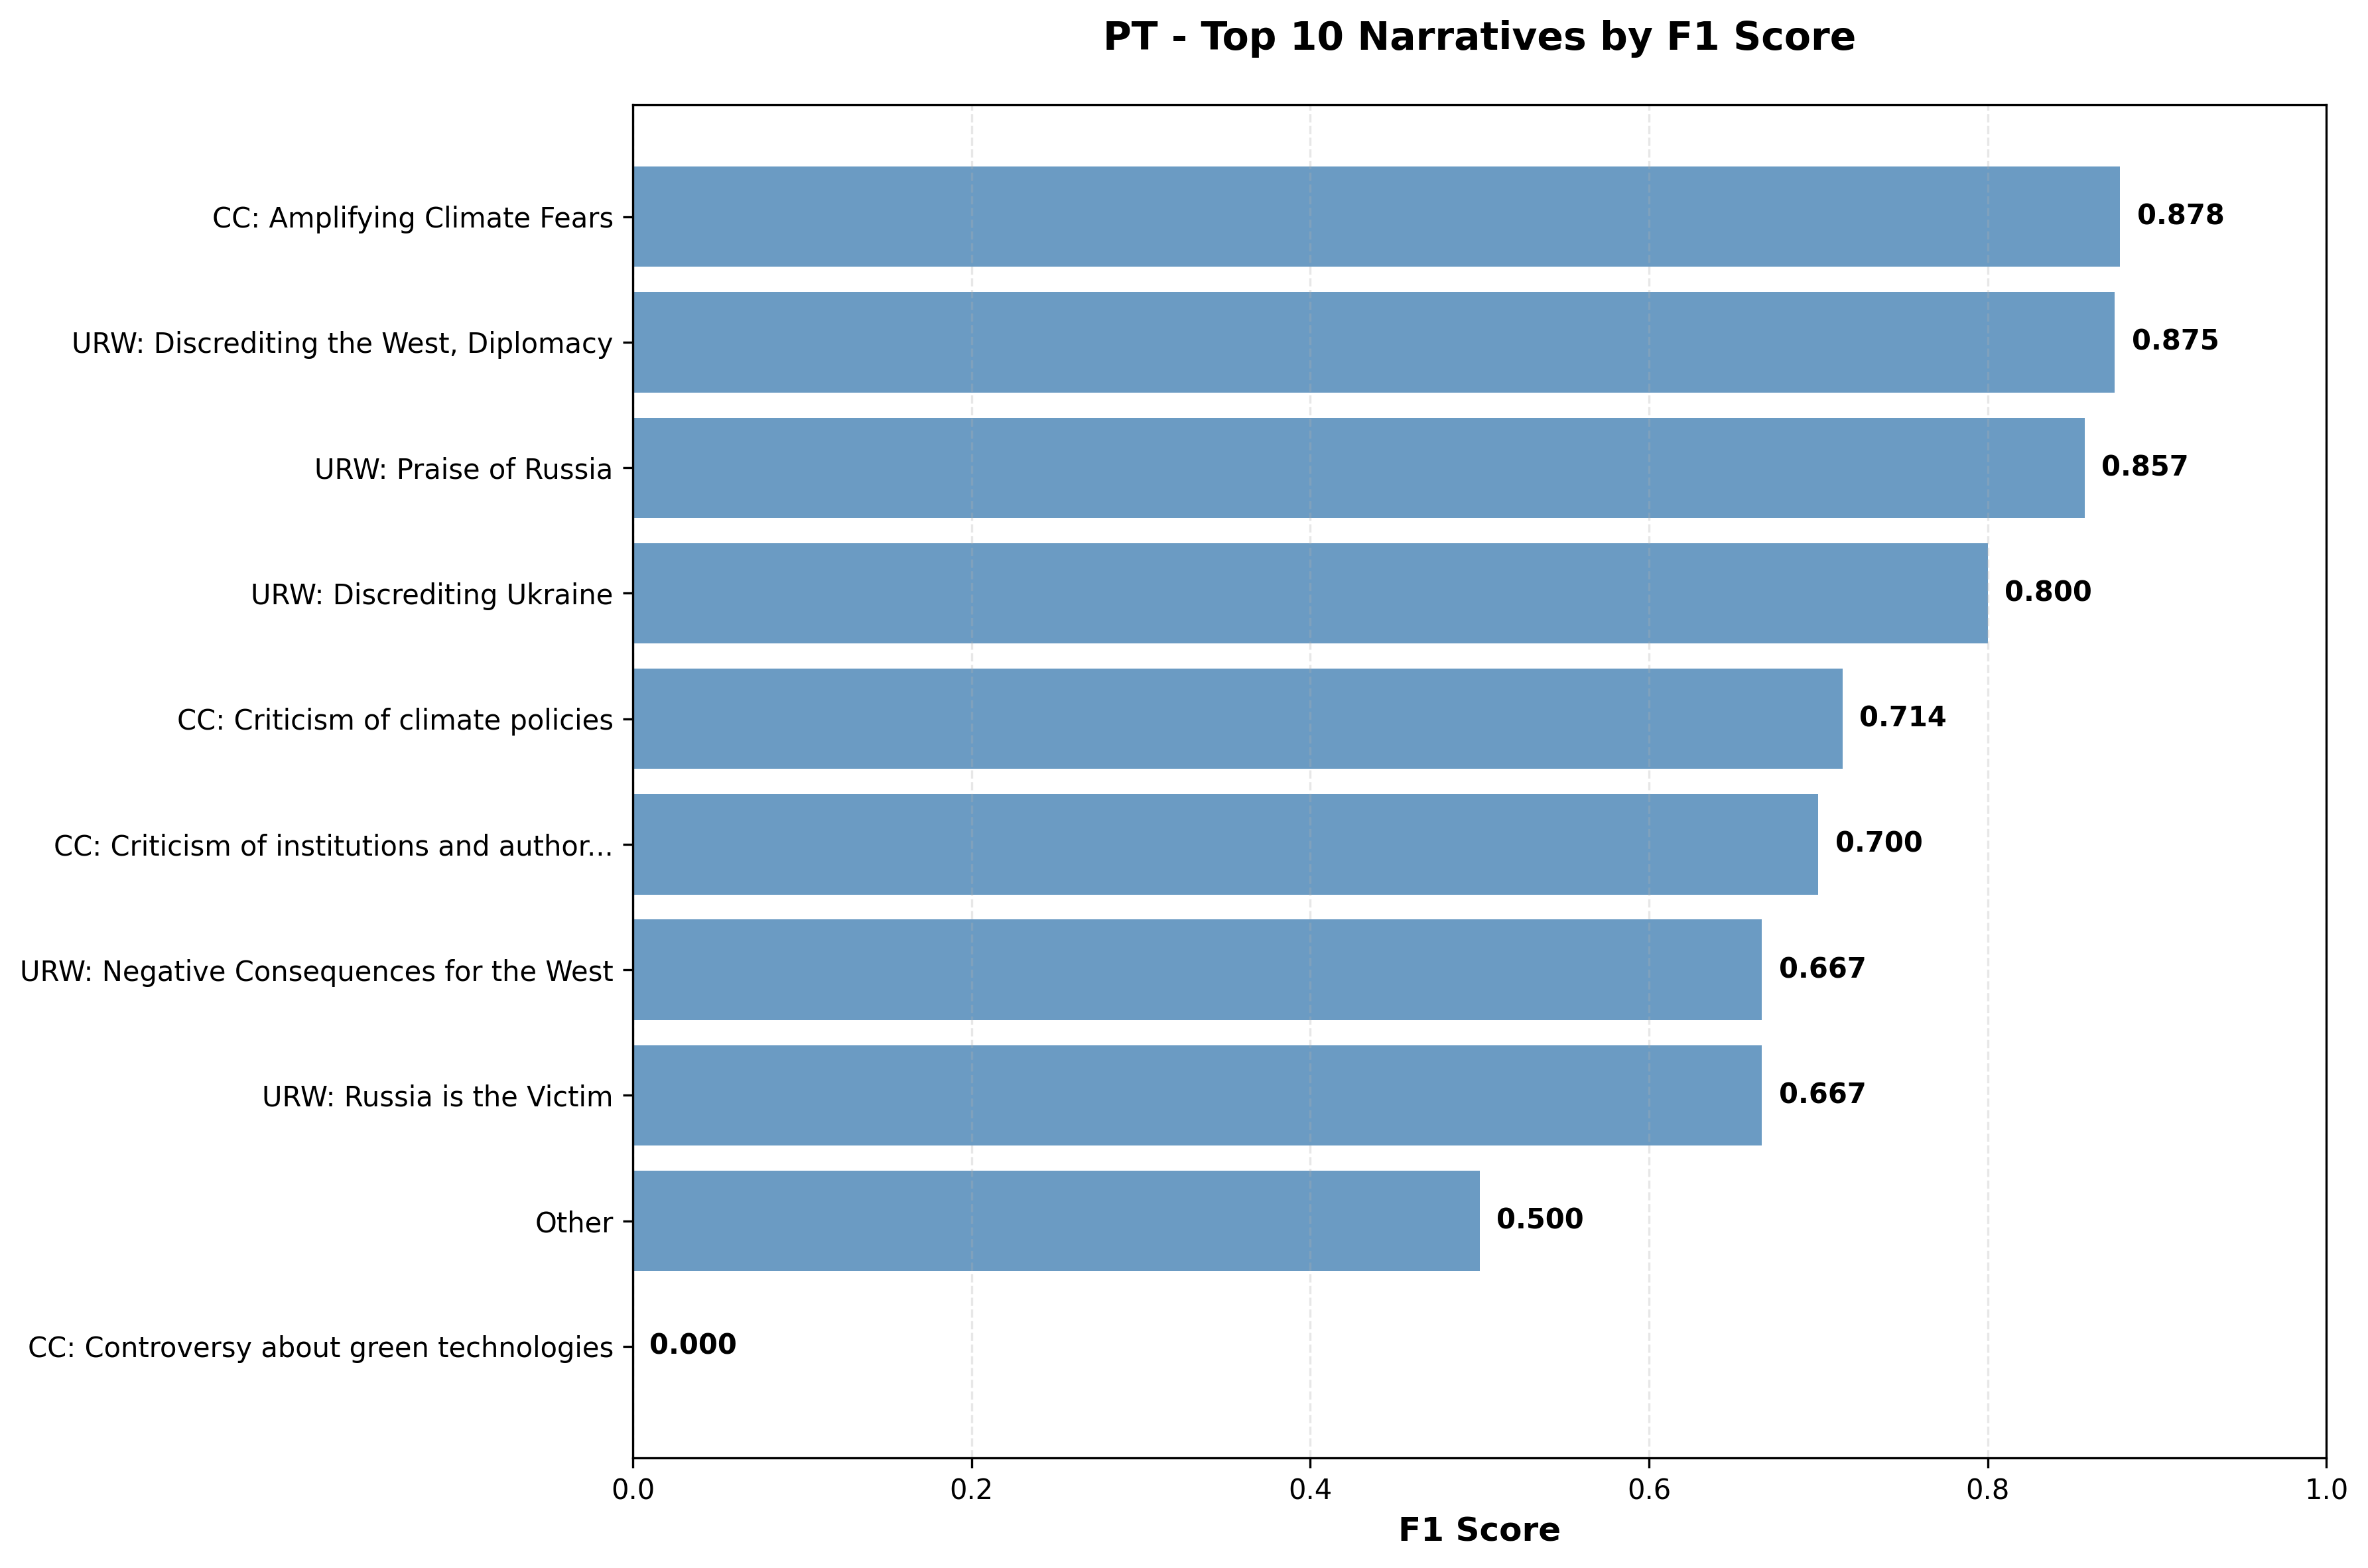
\includegraphics[width=\textwidth]{gemini25_flash_devset_evaluation/plots/PT_top_narratives_f1_scores.png}
        \caption{Top narrative F1 scores}
        \label{fig:app-no-val-pt-narr}
    \end{subfigure}
    \hfill
    \begin{subfigure}[b]{0.48\textwidth}
        \centering
        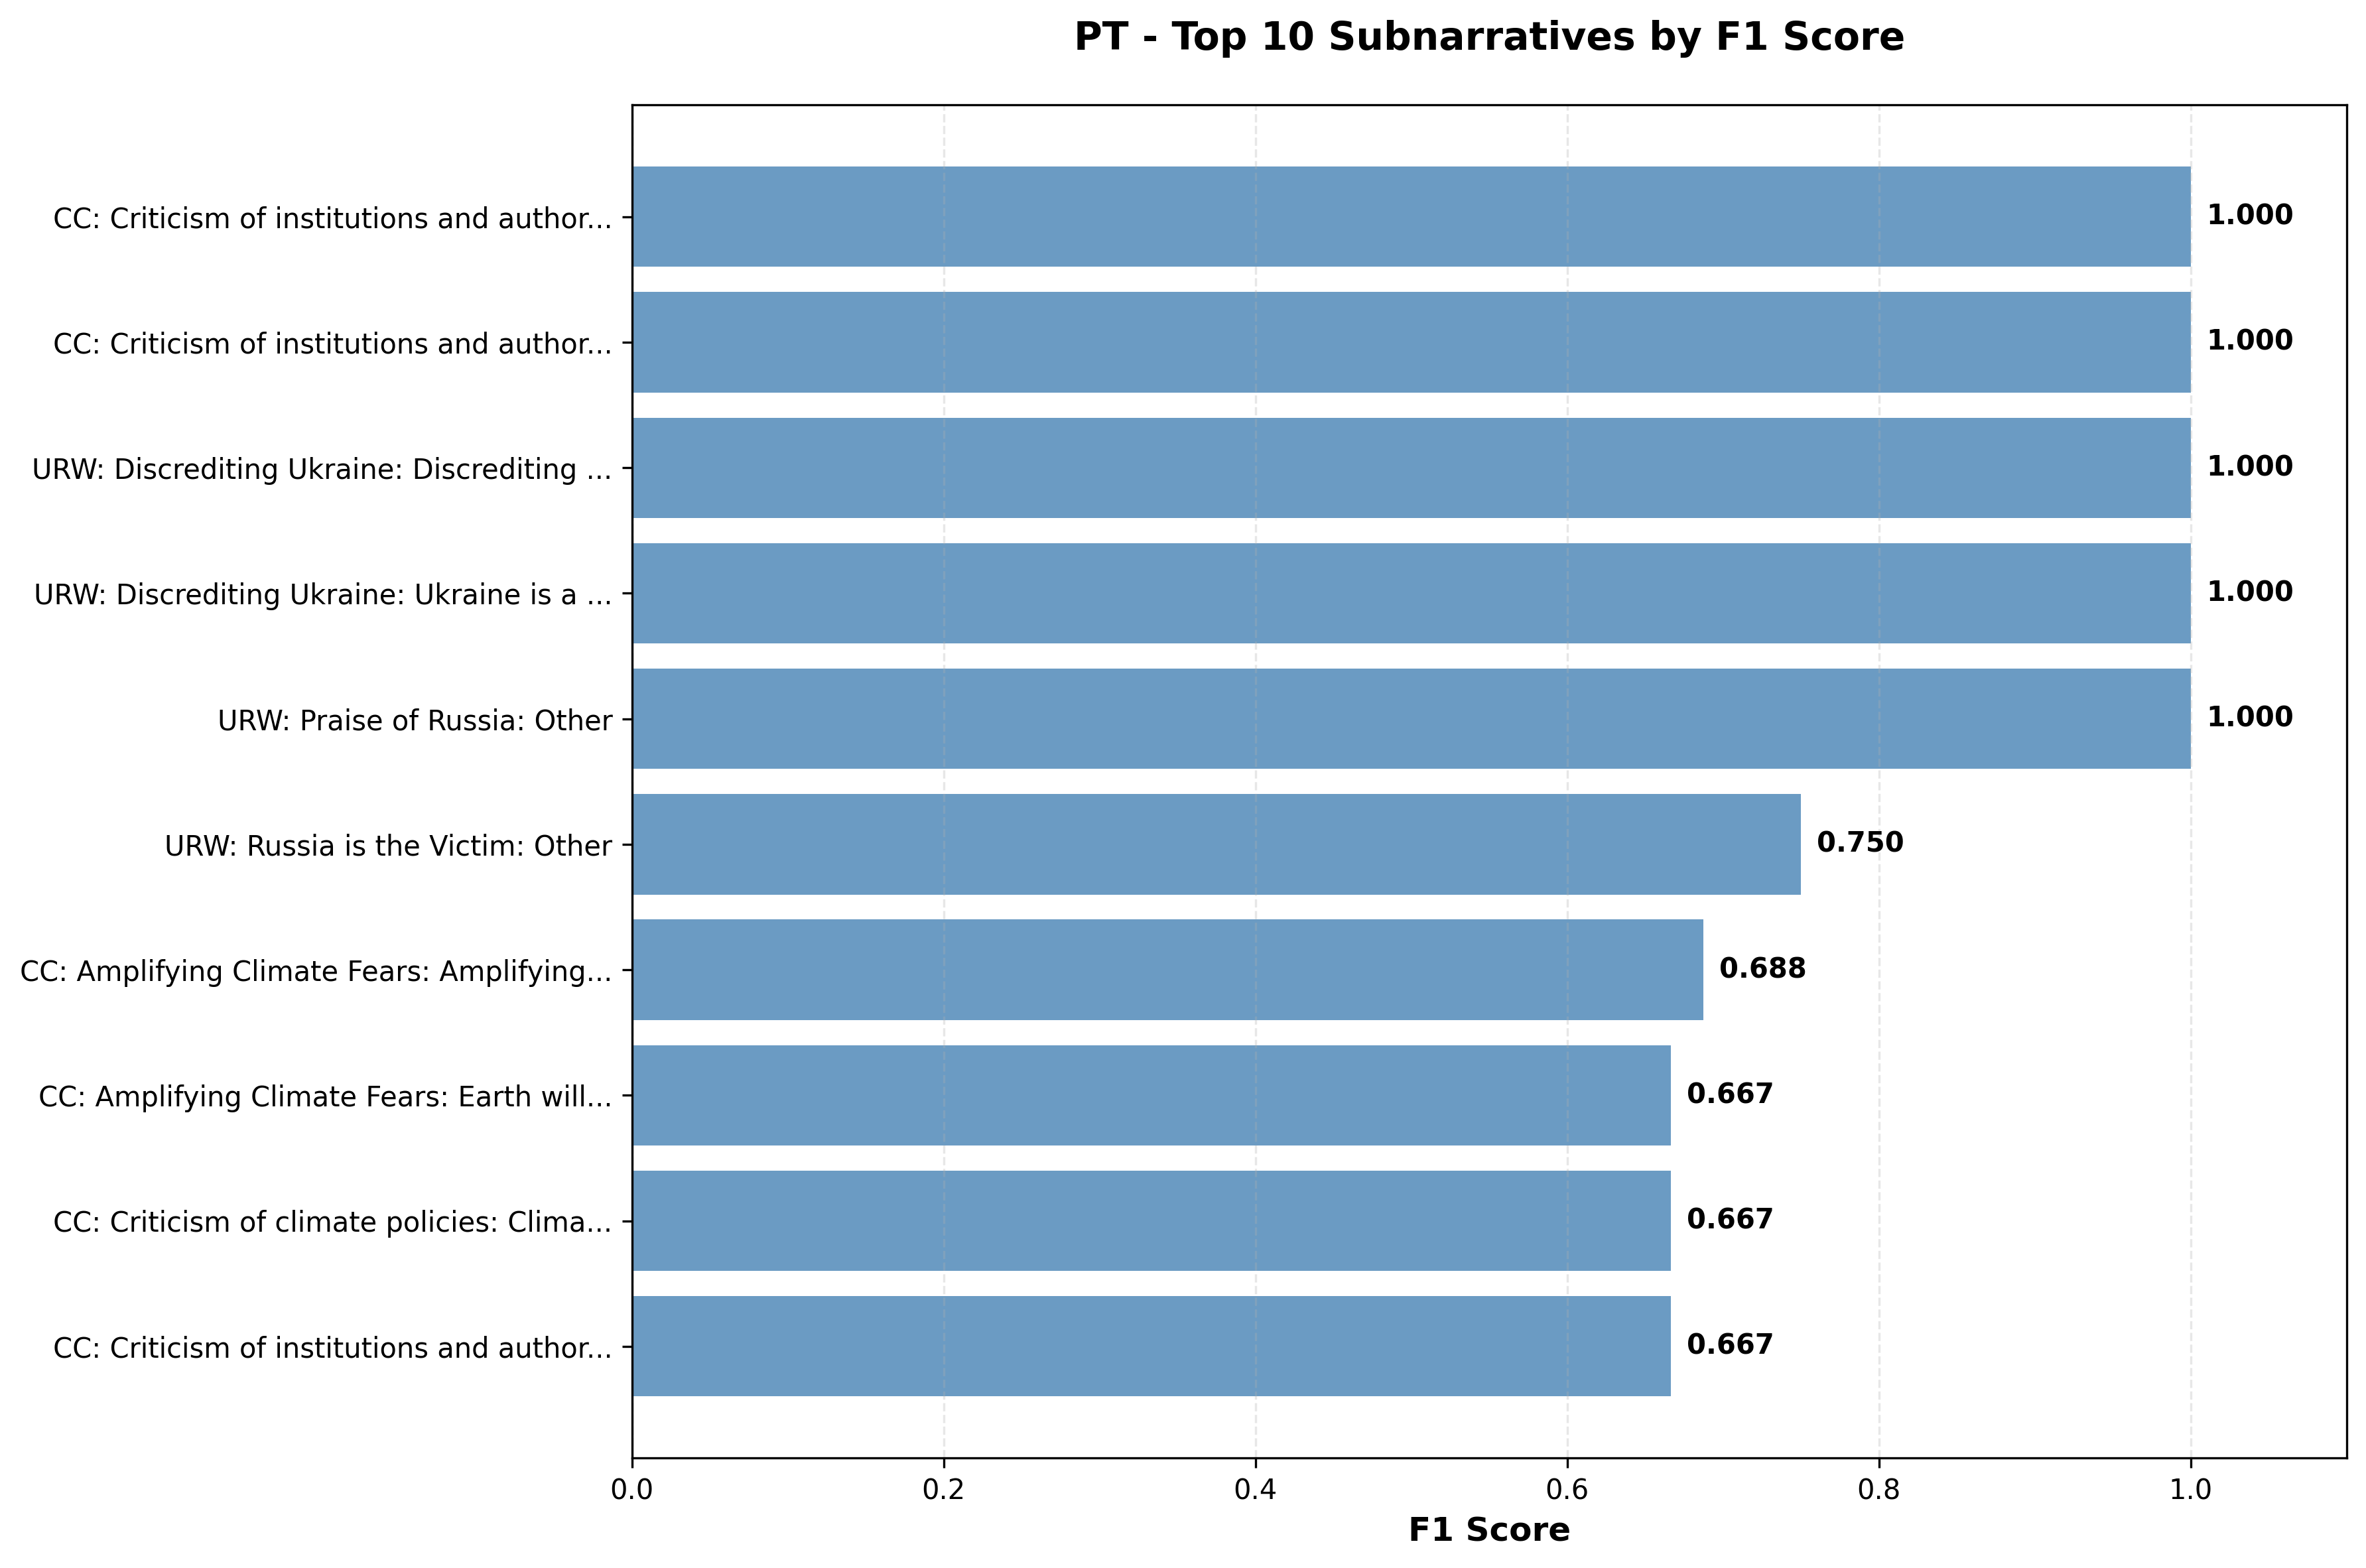
\includegraphics[width=\textwidth]{gemini25_flash_devset_evaluation/plots/PT_top_subnarratives_f1_scores.png}
        \caption{Top subnarrative F1 scores}
        \label{fig:app-no-val-pt-subnarr}
    \end{subfigure}
    \caption{Portuguese performance breakdown for no-validation configuration.}
    \label{fig:app-no-val-pt}
\end{figure}

\subsection{Russian (RU) Performance}

\begin{figure}[H]
    \centering
    \begin{subfigure}[b]{0.48\textwidth}
        \centering
        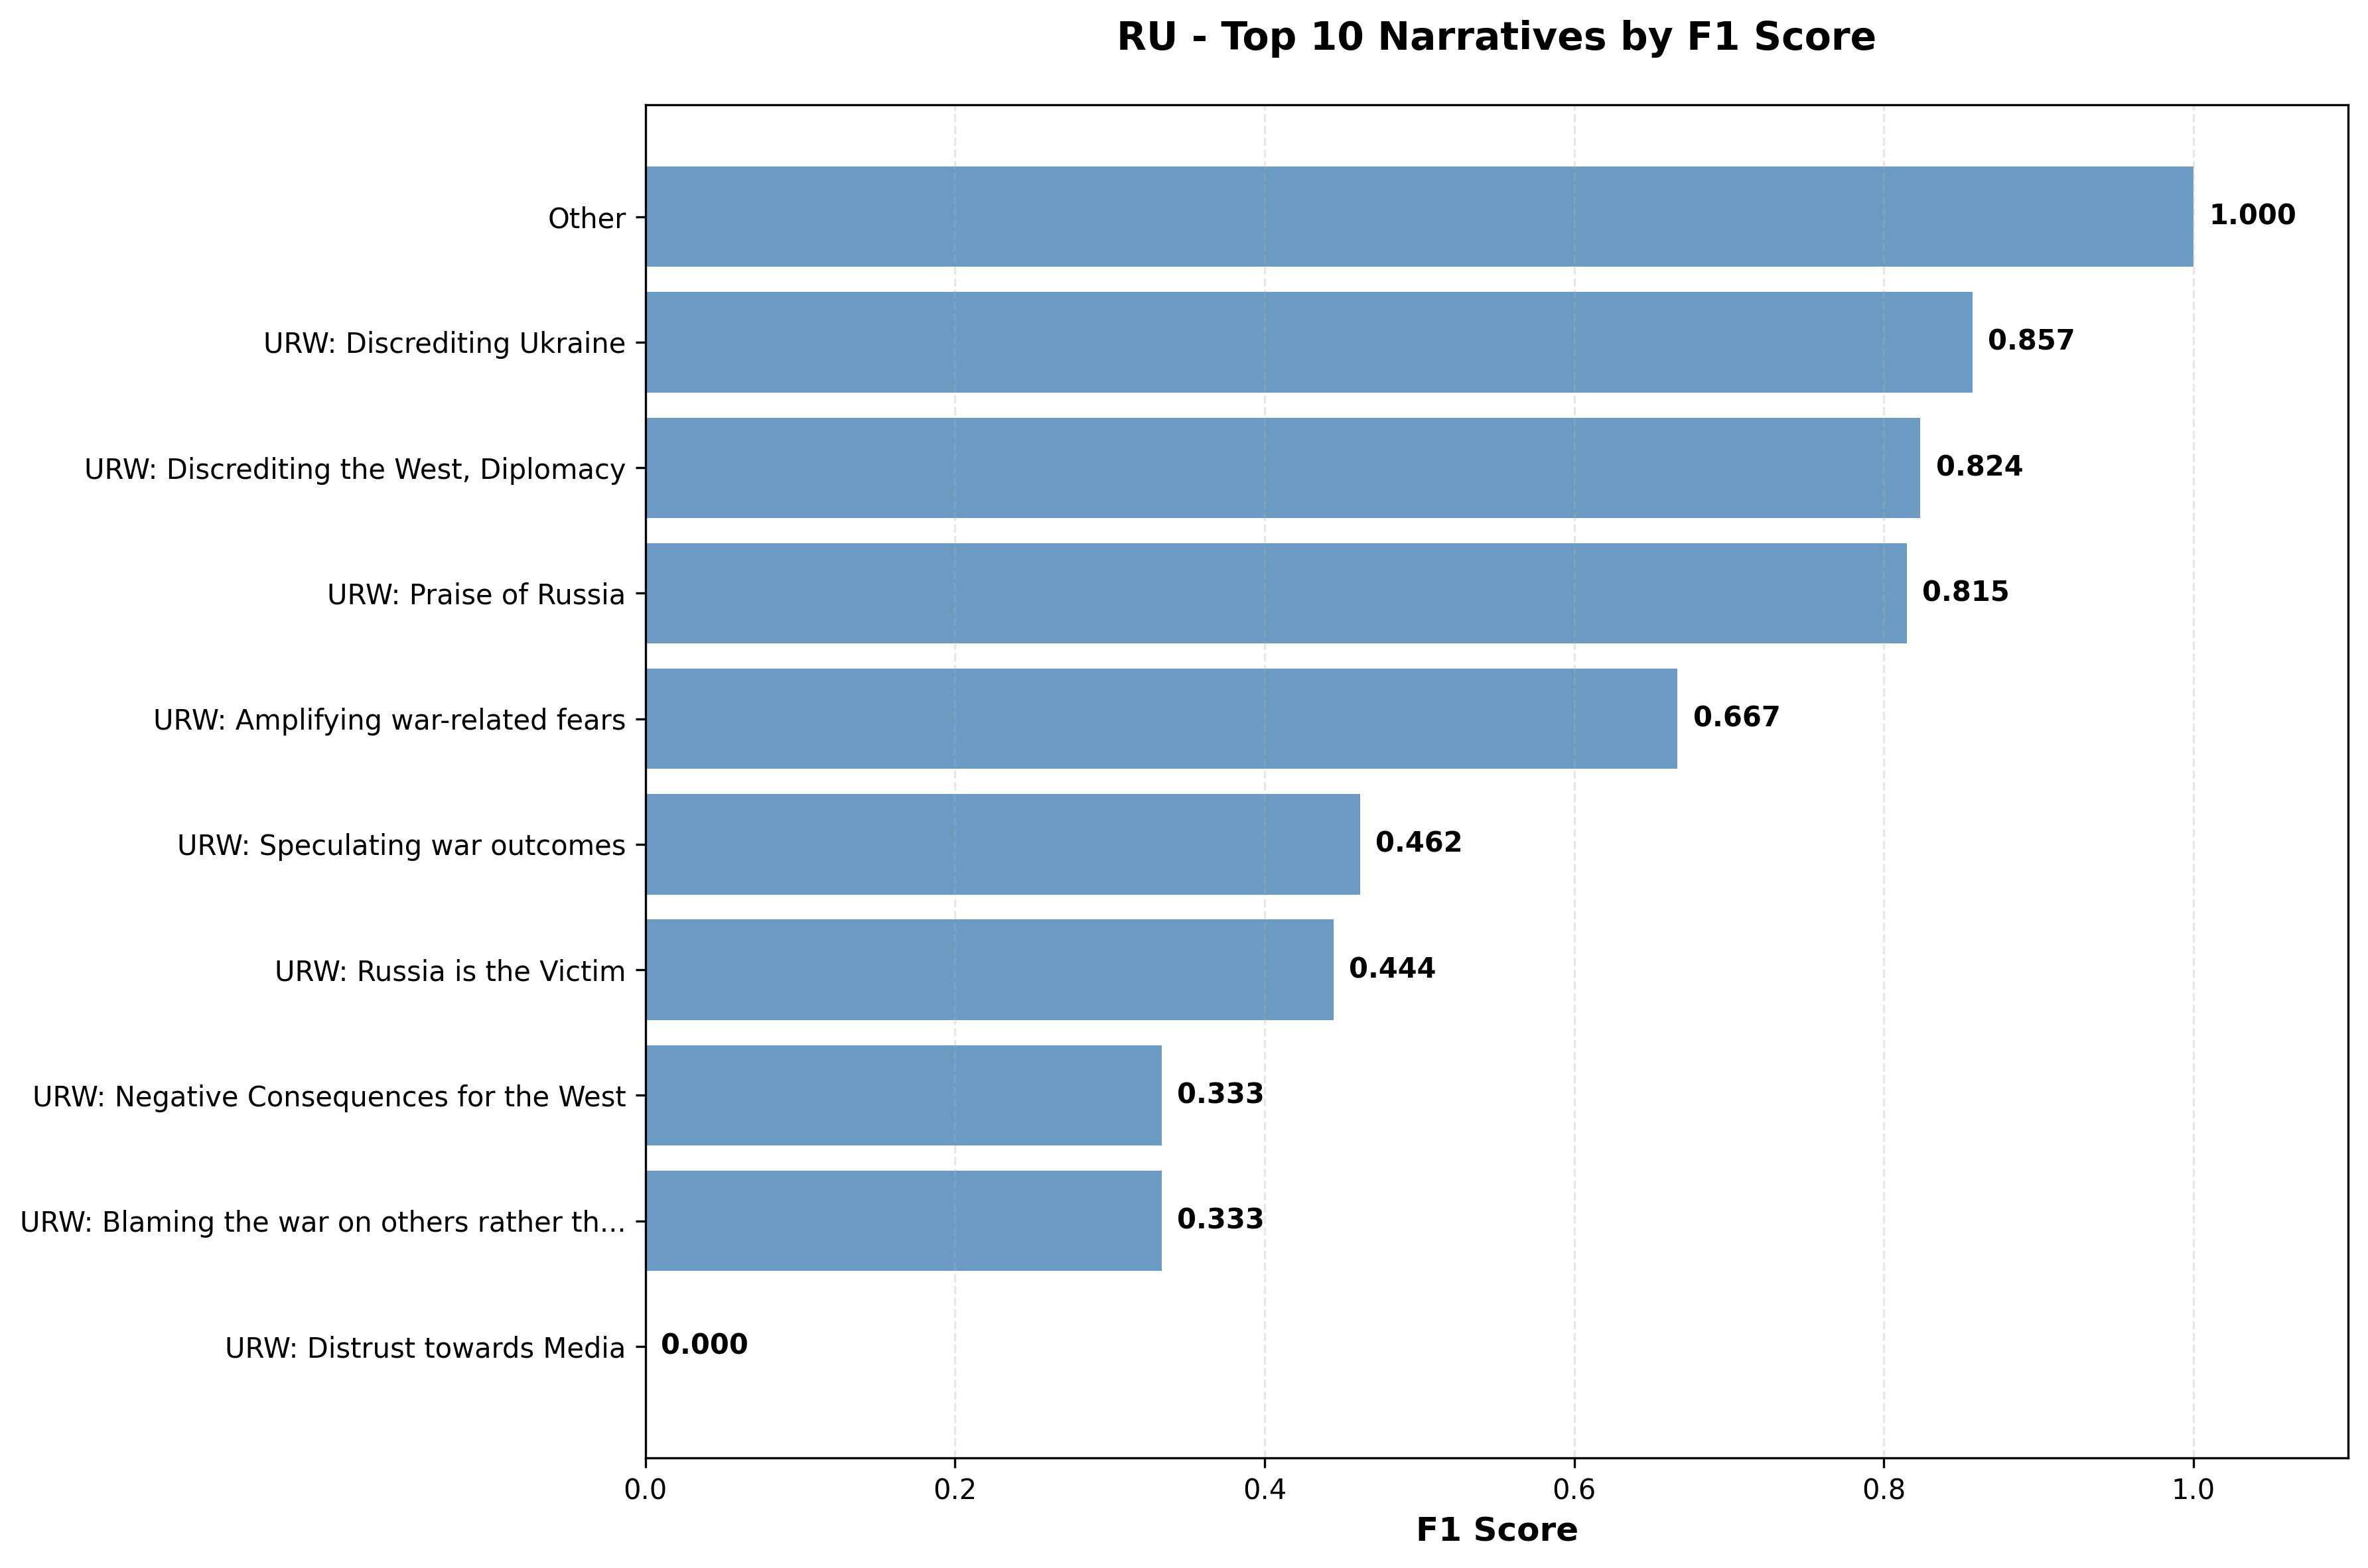
\includegraphics[width=\textwidth]{gemini25_flash_devset_evaluation/plots/RU_top_narratives_f1_scores.png}
        \caption{Top narrative F1 scores}
        \label{fig:app-no-val-ru-narr}
    \end{subfigure}
    \hfill
    \begin{subfigure}[b]{0.48\textwidth}
        \centering
        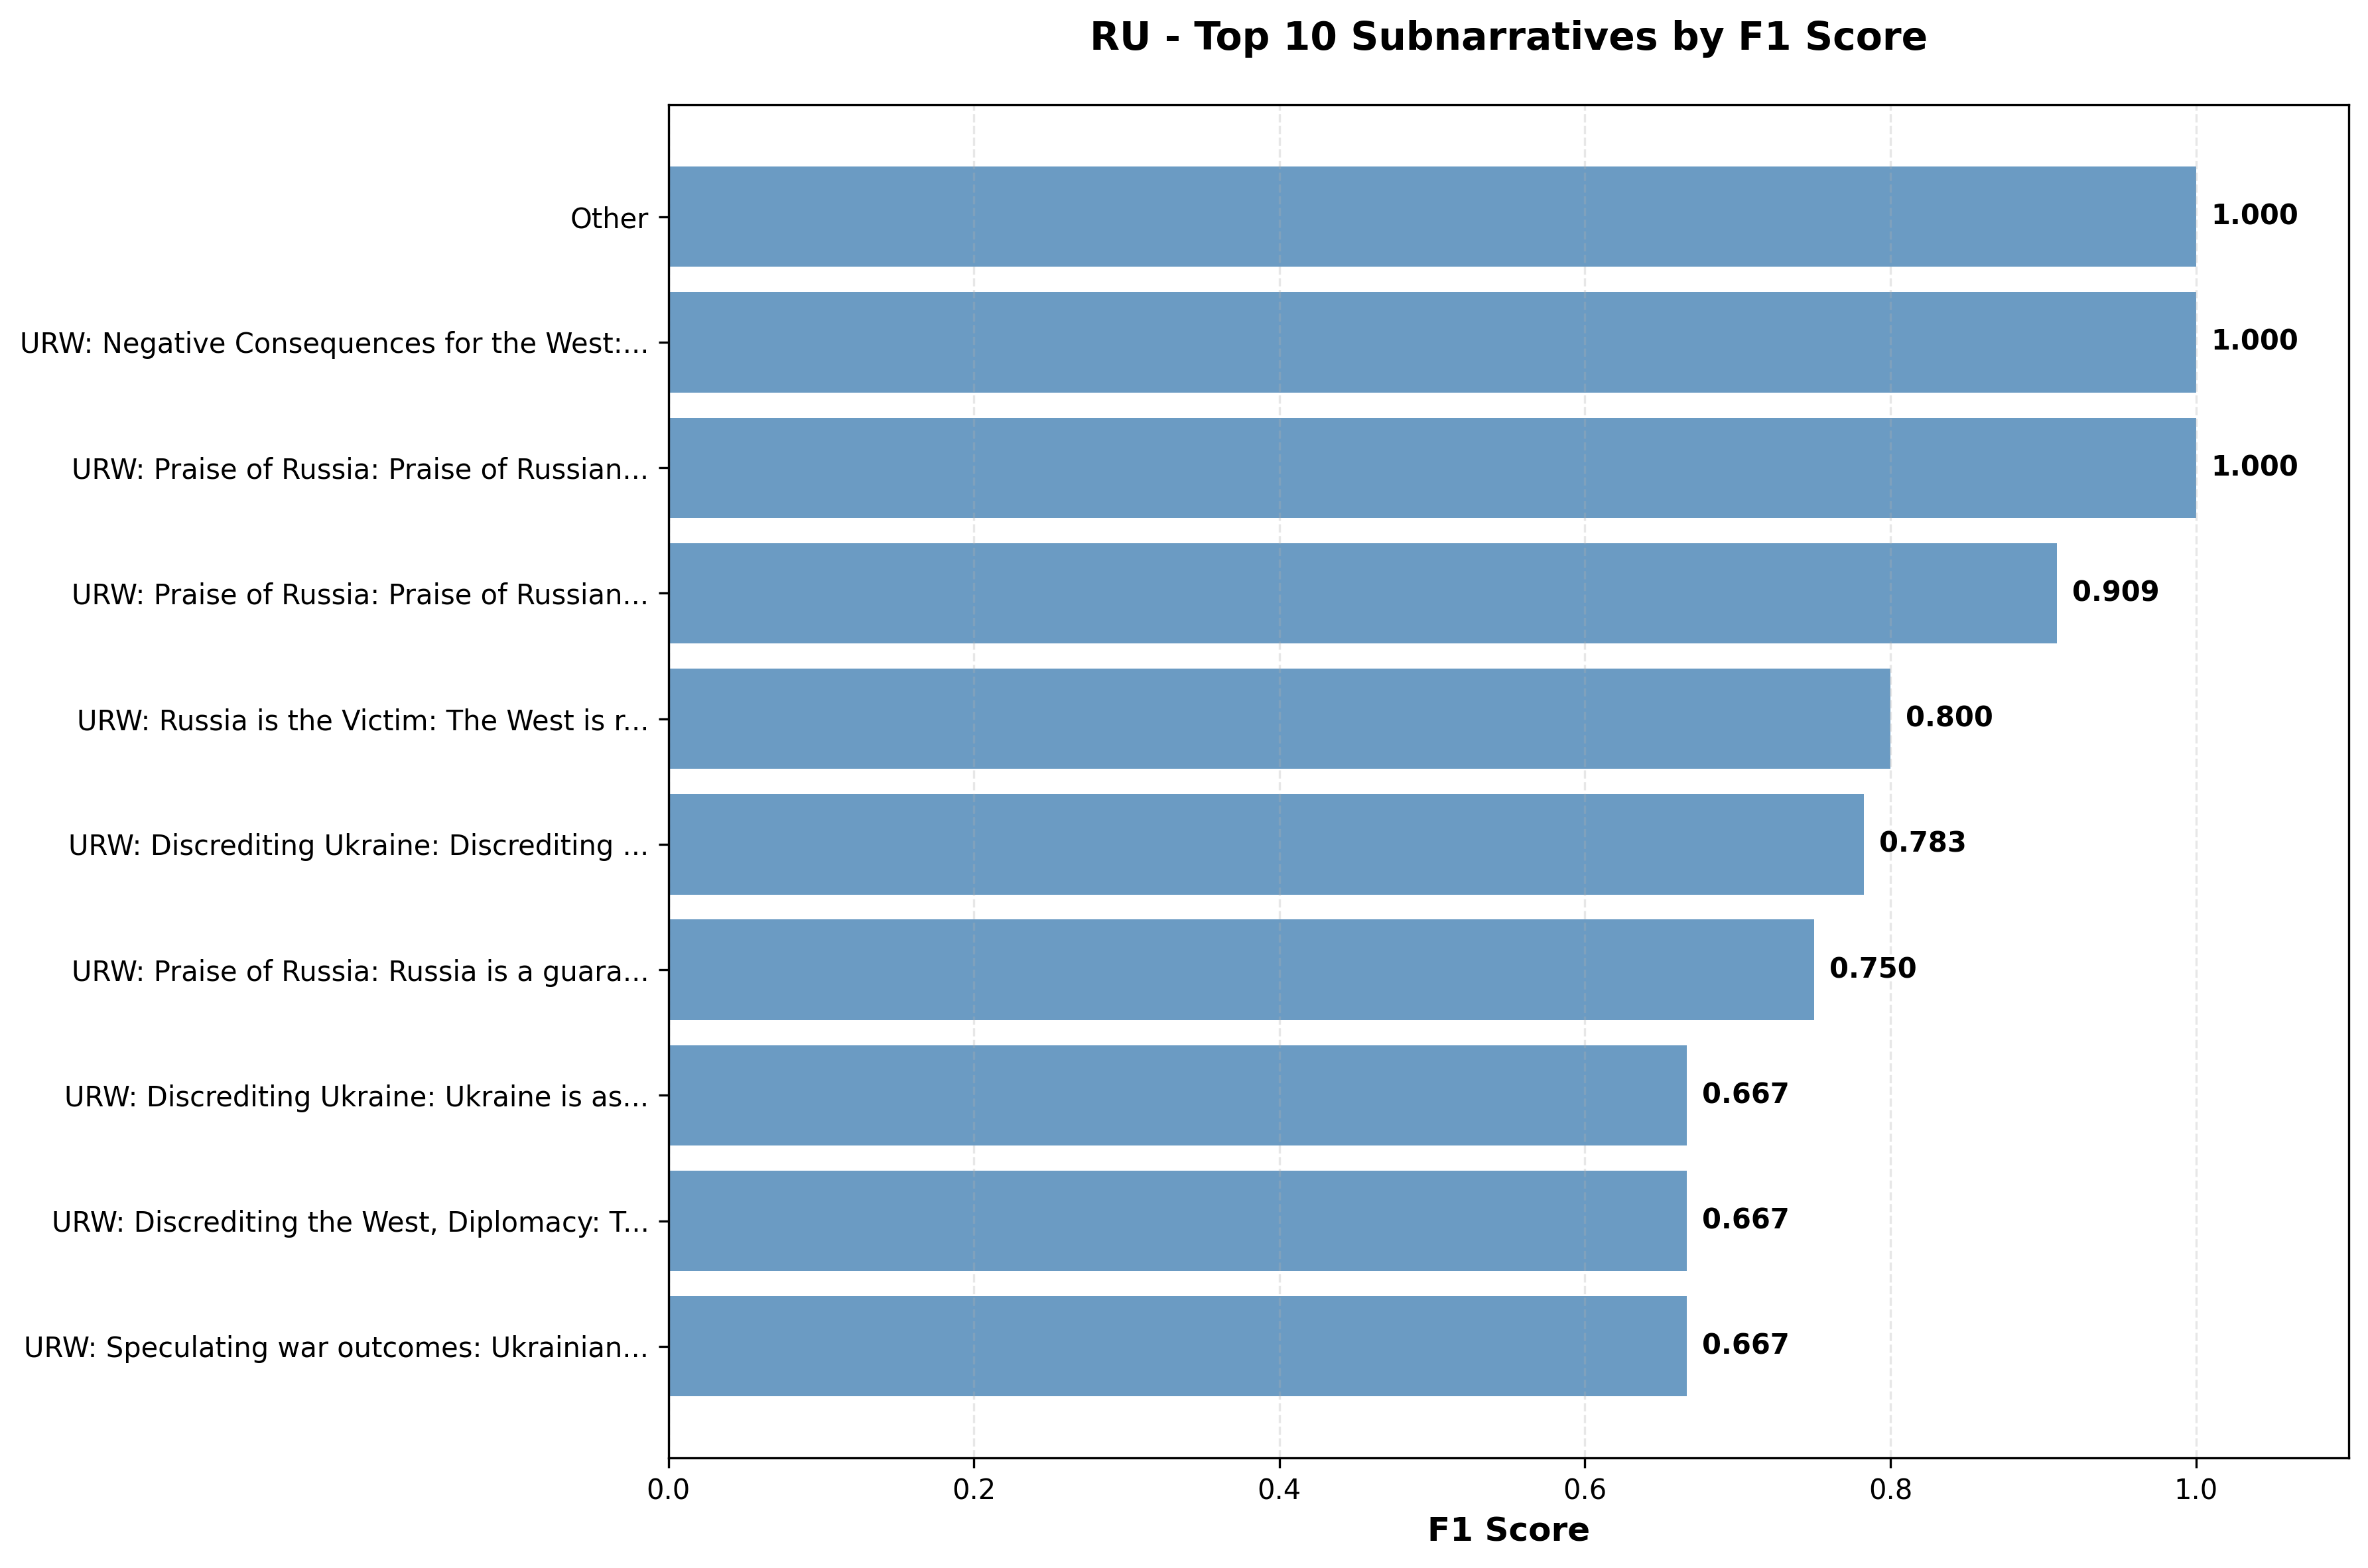
\includegraphics[width=\textwidth]{gemini25_flash_devset_evaluation/plots/RU_top_subnarratives_f1_scores.png}
        \caption{Top subnarrative F1 scores}
        \label{fig:app-no-val-ru-subnarr}
    \end{subfigure}
    \caption{Russian performance breakdown for no-validation configuration.}
    \label{fig:app-no-val-ru}
\end{figure}

\clearpage
\section{Architecture 2: Narrative Validation Configuration}
\label{app:narr-validation}

This section presents results from the Actor-Critique pipeline with narrative-level validation enabled.

\subsection{Overall Performance Comparison}

\begin{figure}[H]
    \centering
    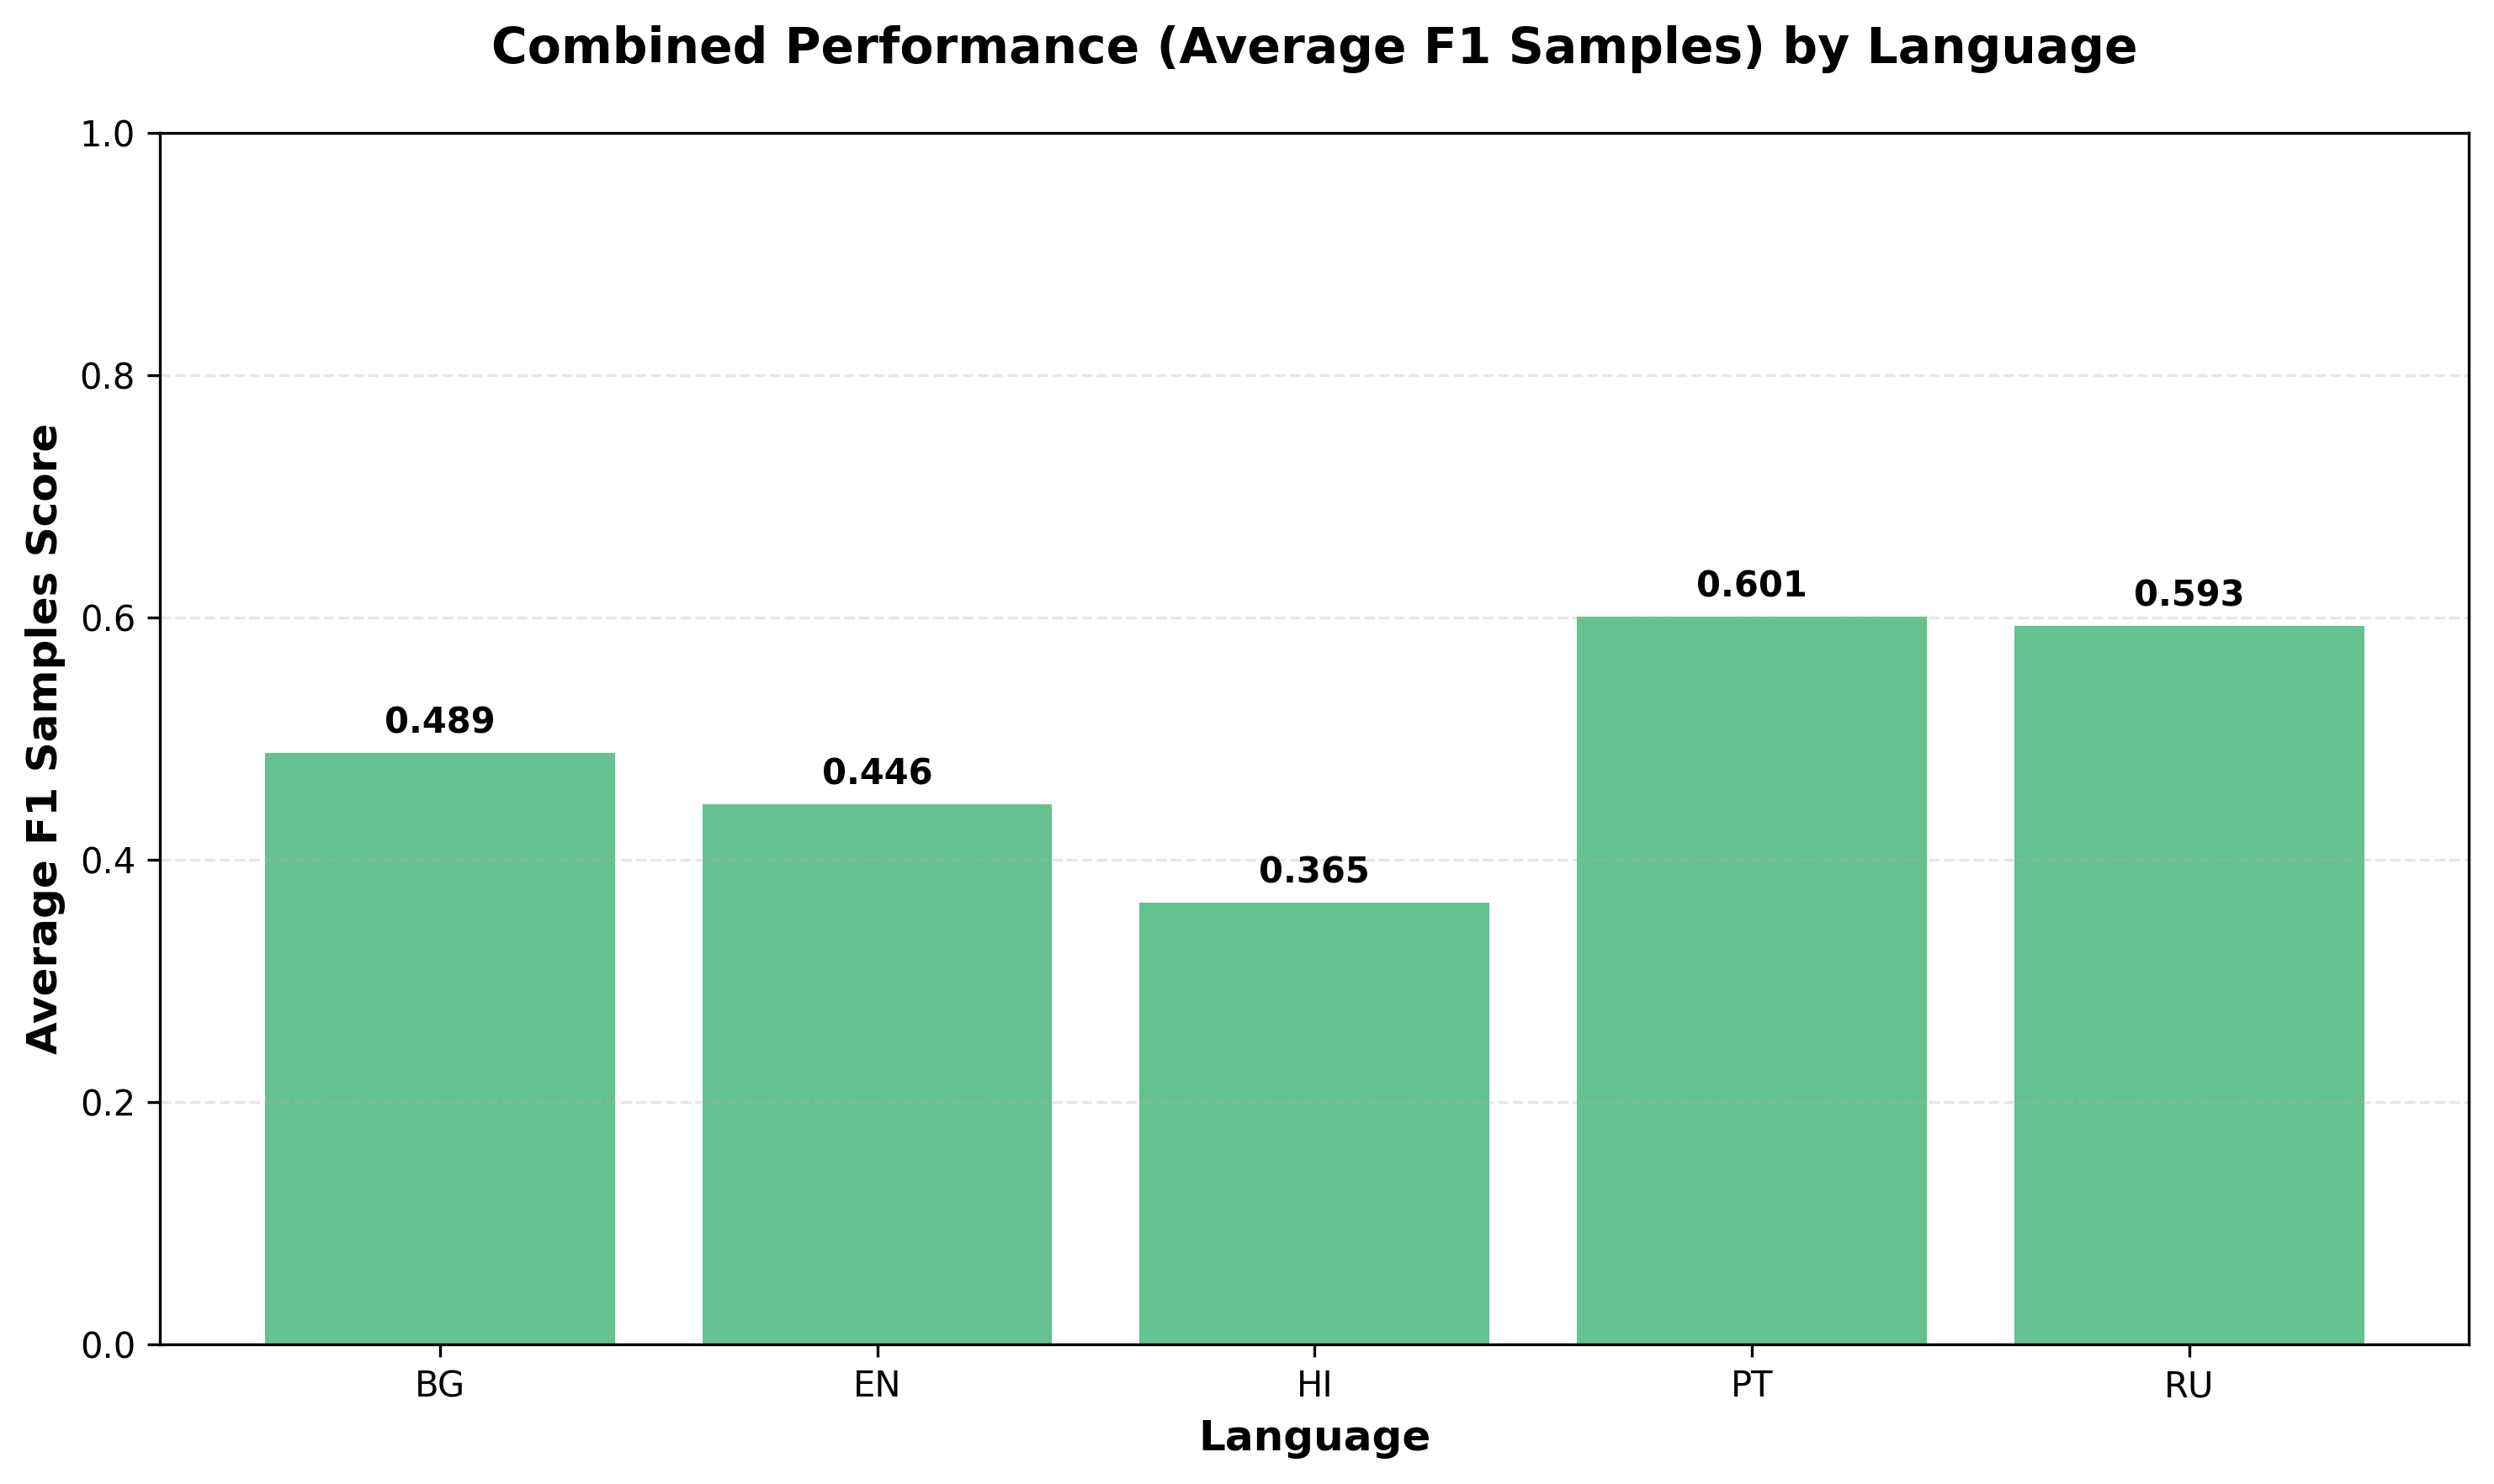
\includegraphics[width=0.85\textwidth]{gemini25_flash_narr_val_evaluation/plots/combined_performance_by_language.png}
    \caption{Combined performance across all languages for the narrative-validation configuration.}
    \label{fig:app-narr-val-combined}
\end{figure}

\begin{figure}[H]
    \centering
    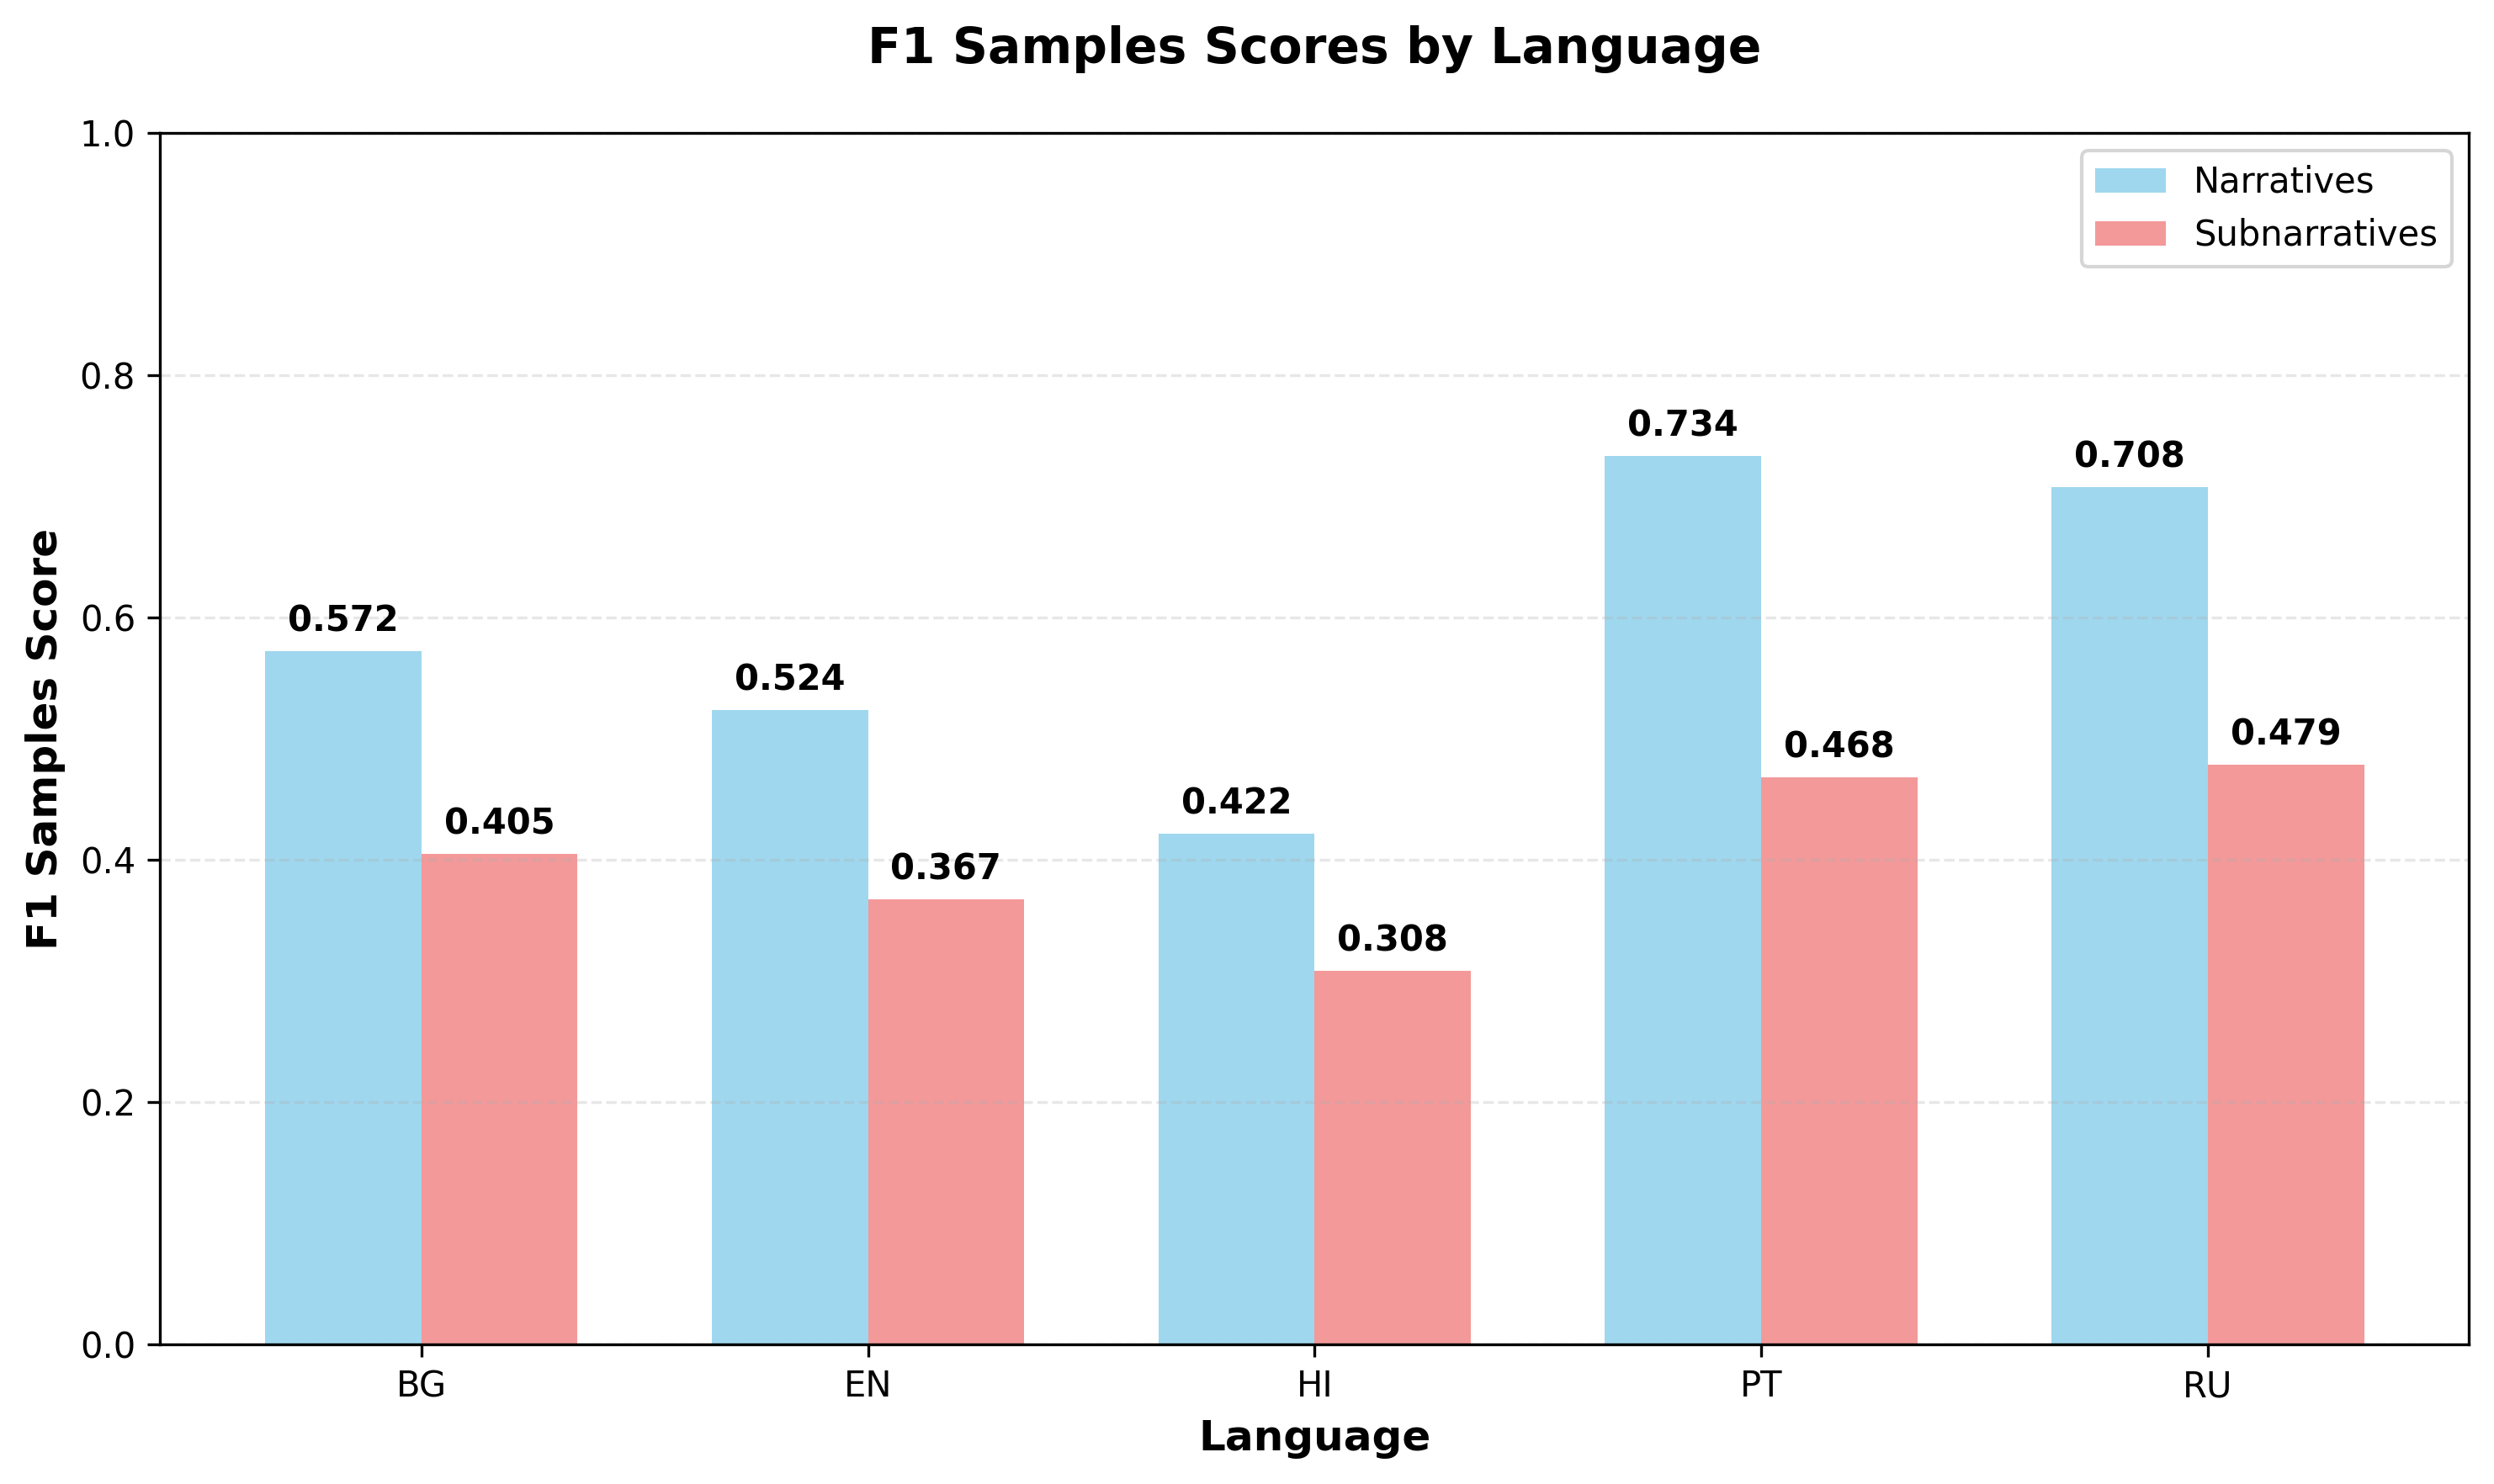
\includegraphics[width=0.85\textwidth]{gemini25_flash_narr_val_evaluation/plots/f1_samples_by_language.png}
    \caption{F1 Samples performance by language for the narrative-validation configuration.}
    \label{fig:app-narr-val-f1-samples}
\end{figure}

\subsection{Bulgarian (BG) Performance}

\begin{figure}[H]
    \centering
    \begin{subfigure}[b]{0.48\textwidth}
        \centering
        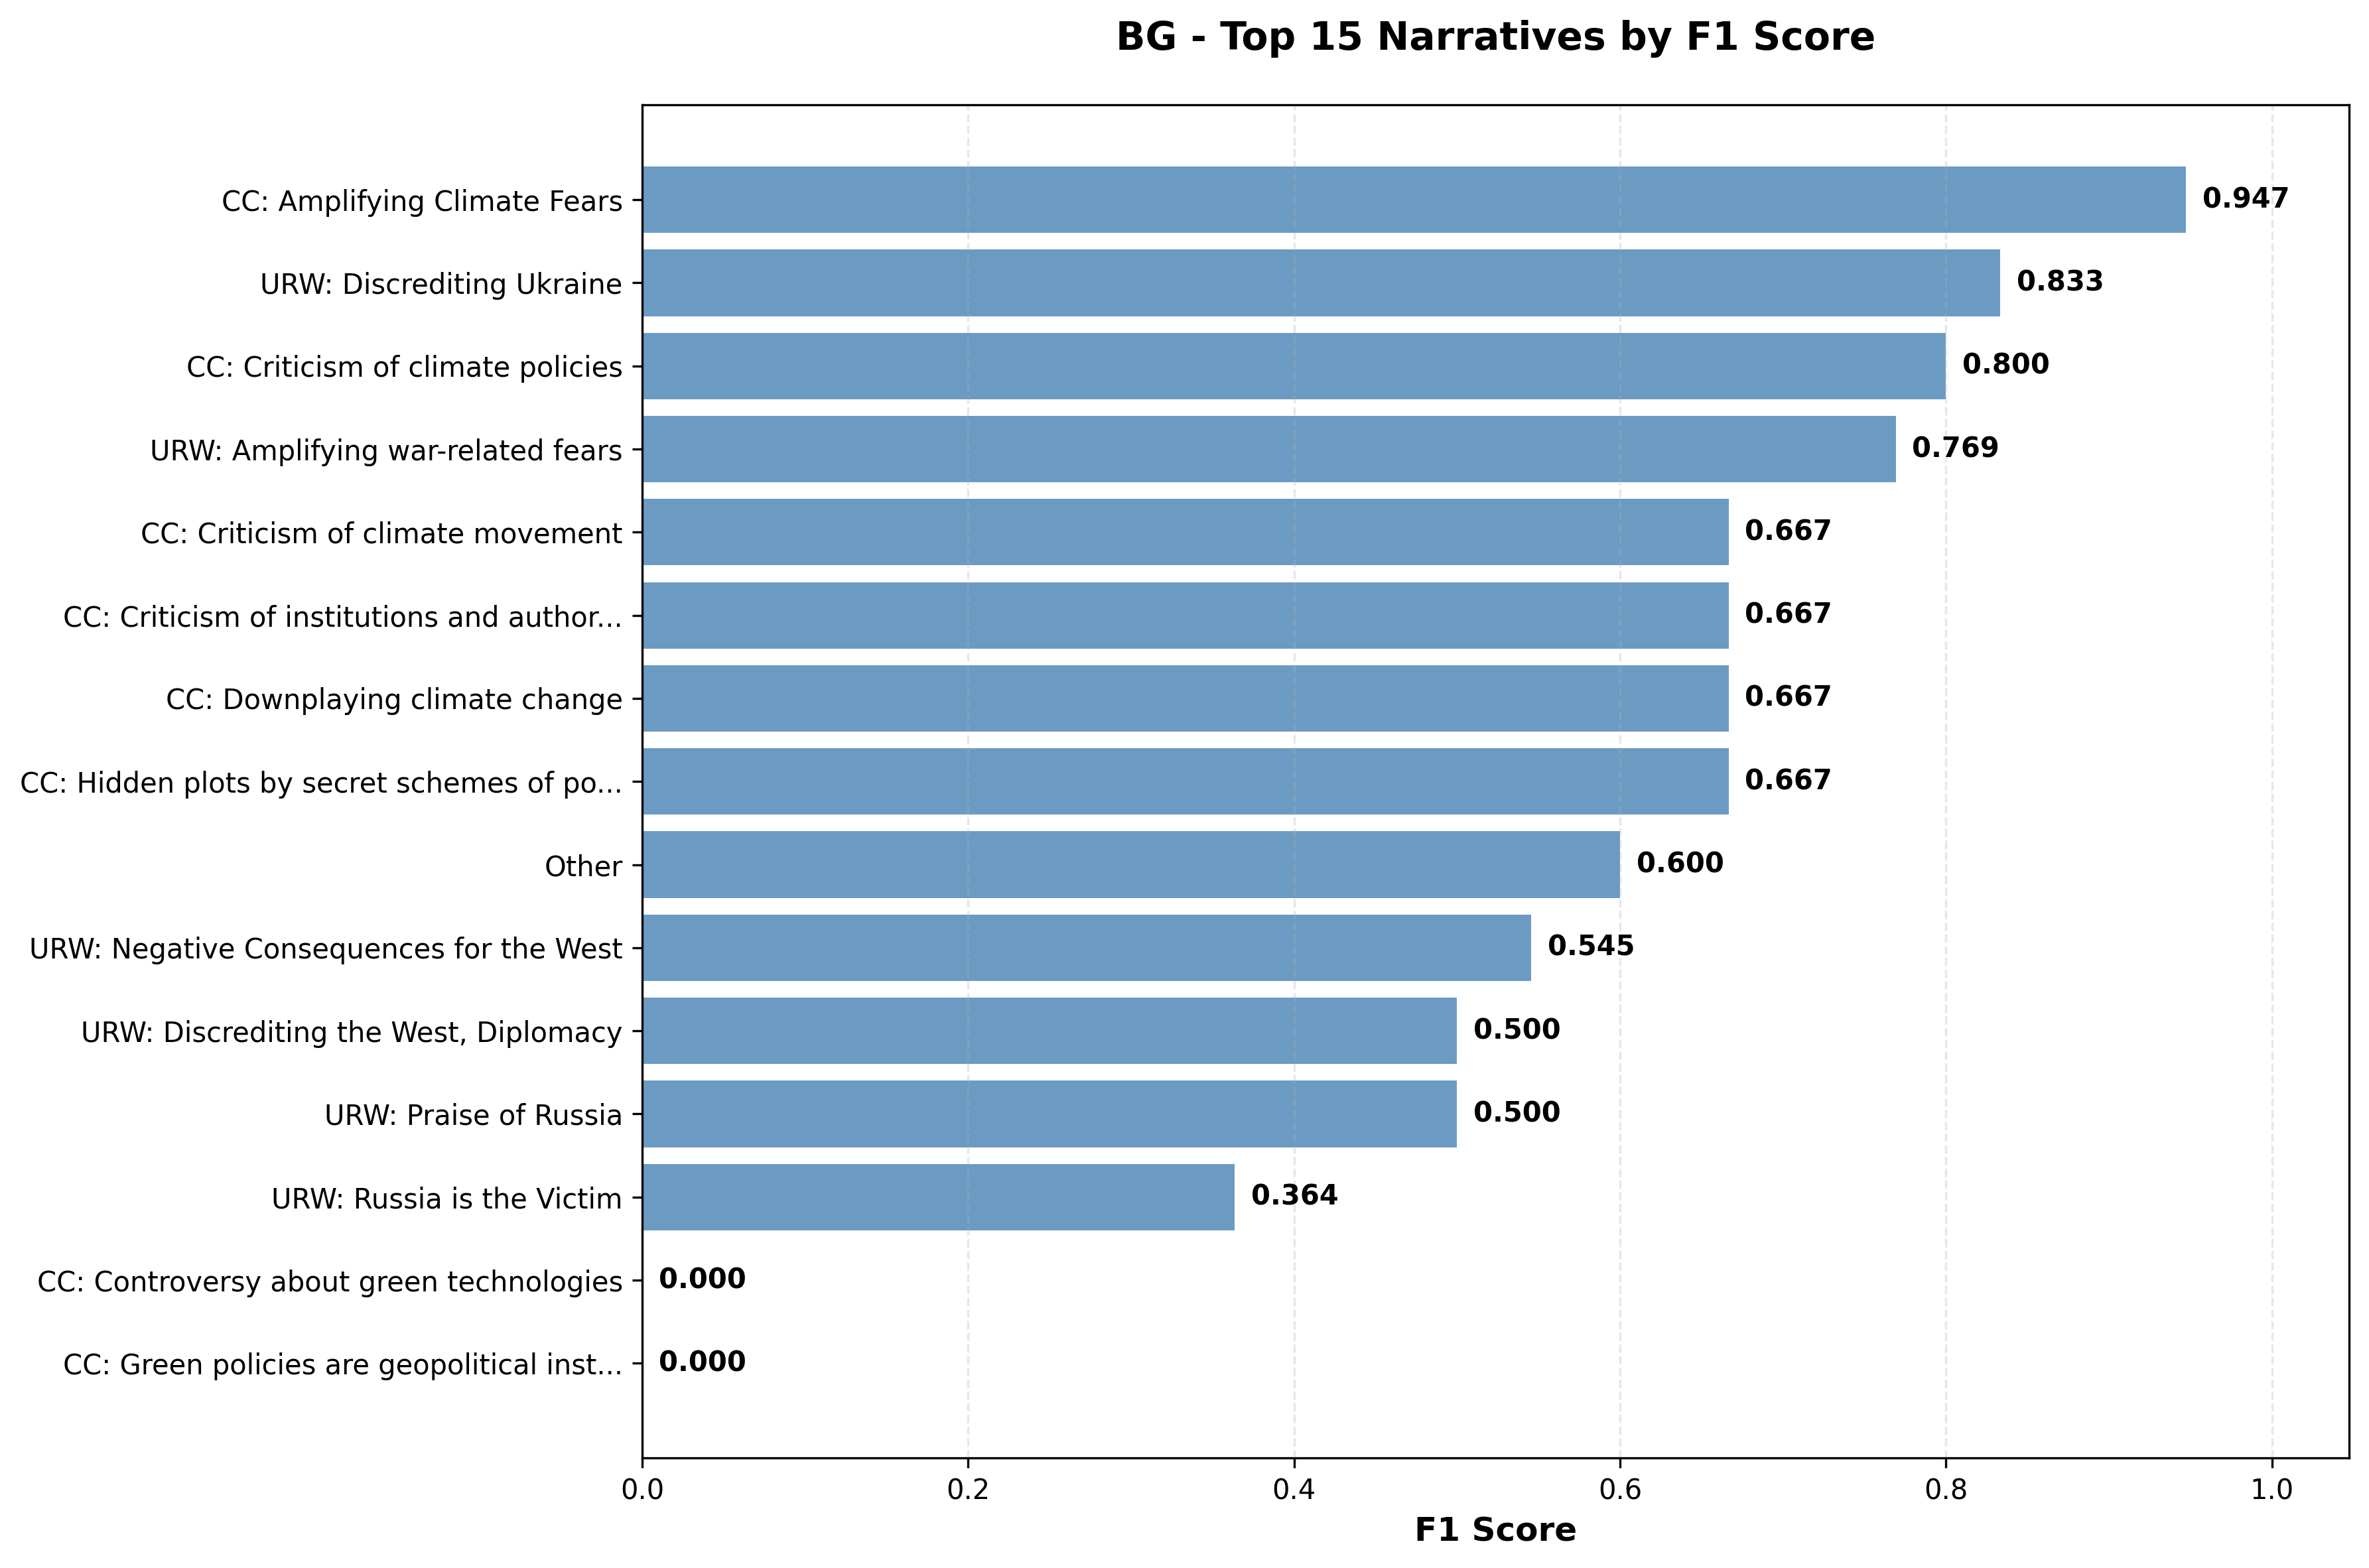
\includegraphics[width=\textwidth]{gemini25_flash_narr_val_evaluation/plots/BG_top_narratives_f1_scores.png}
        \caption{Top narrative F1 scores}
        \label{fig:app-narr-val-bg-narr}
    \end{subfigure}
    \hfill
    \begin{subfigure}[b]{0.48\textwidth}
        \centering
        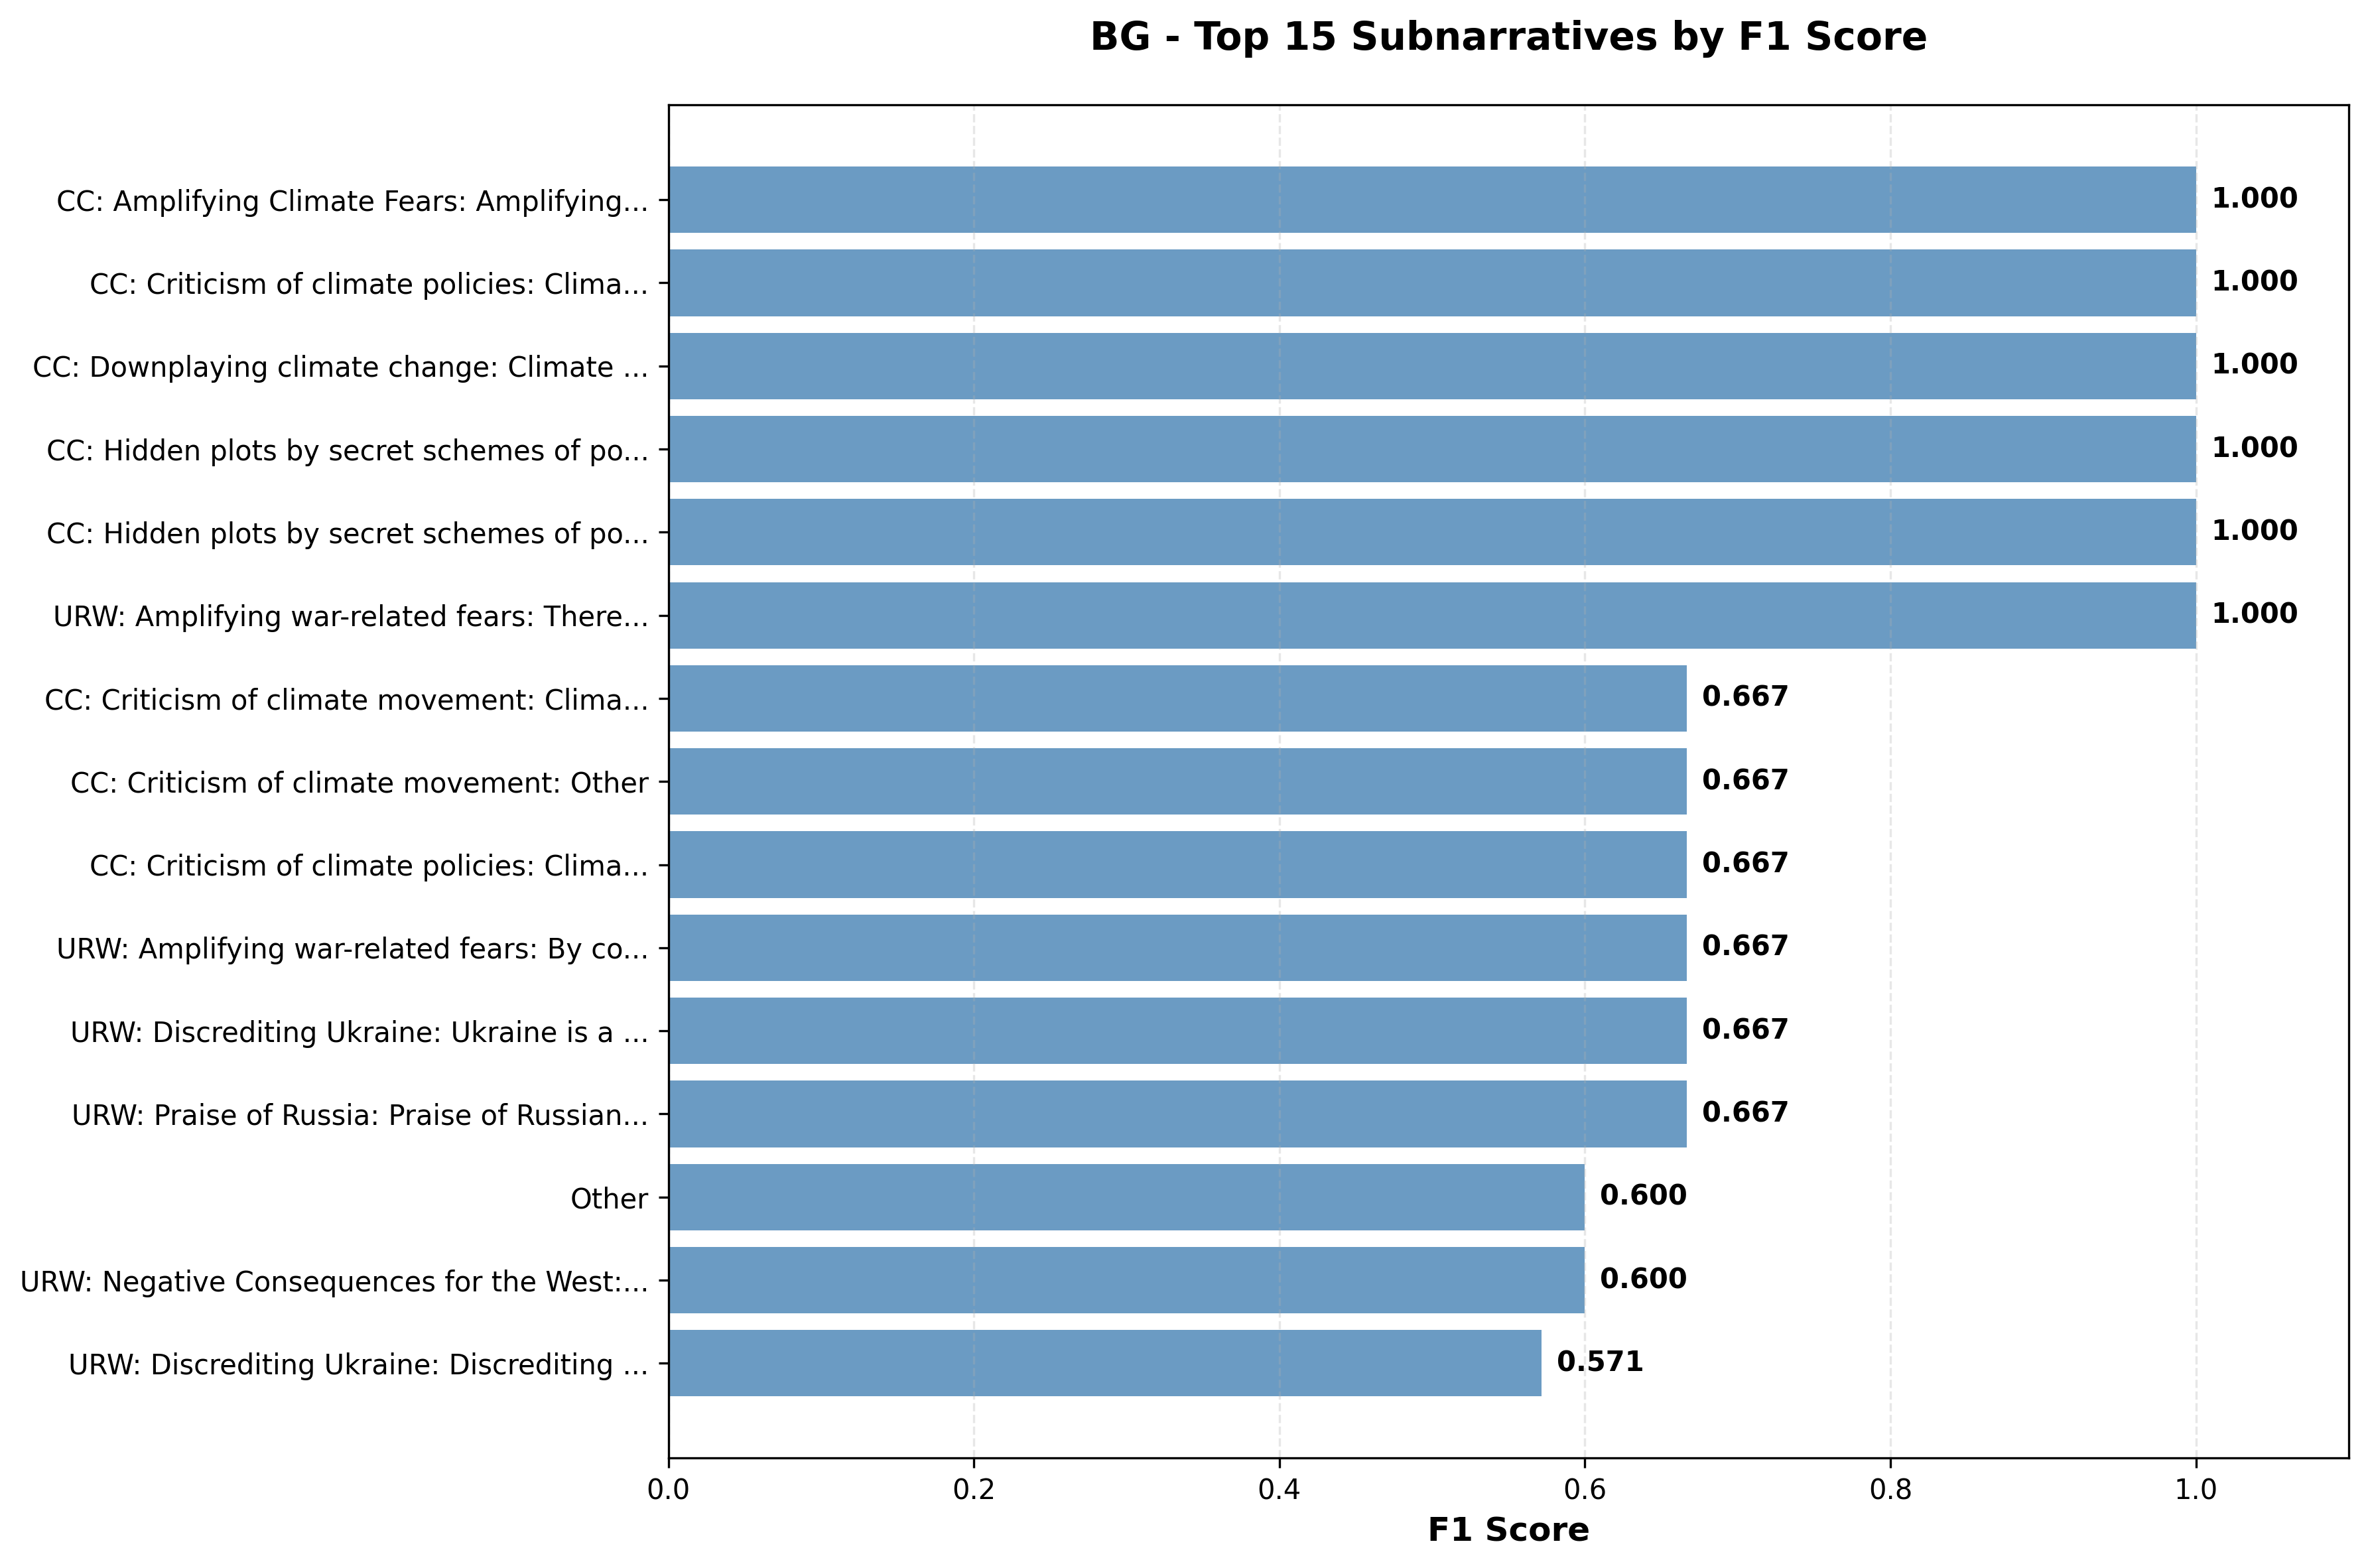
\includegraphics[width=\textwidth]{gemini25_flash_narr_val_evaluation/plots/BG_top_subnarratives_f1_scores.png}
        \caption{Top subnarrative F1 scores}
        \label{fig:app-narr-val-bg-subnarr}
    \end{subfigure}
    \caption{Bulgarian performance breakdown for narrative-validation configuration.}
    \label{fig:app-narr-val-bg}
\end{figure}

\subsection{English (EN) Performance}

\begin{figure}[H]
    \centering
    \begin{subfigure}[b]{0.48\textwidth}
        \centering
        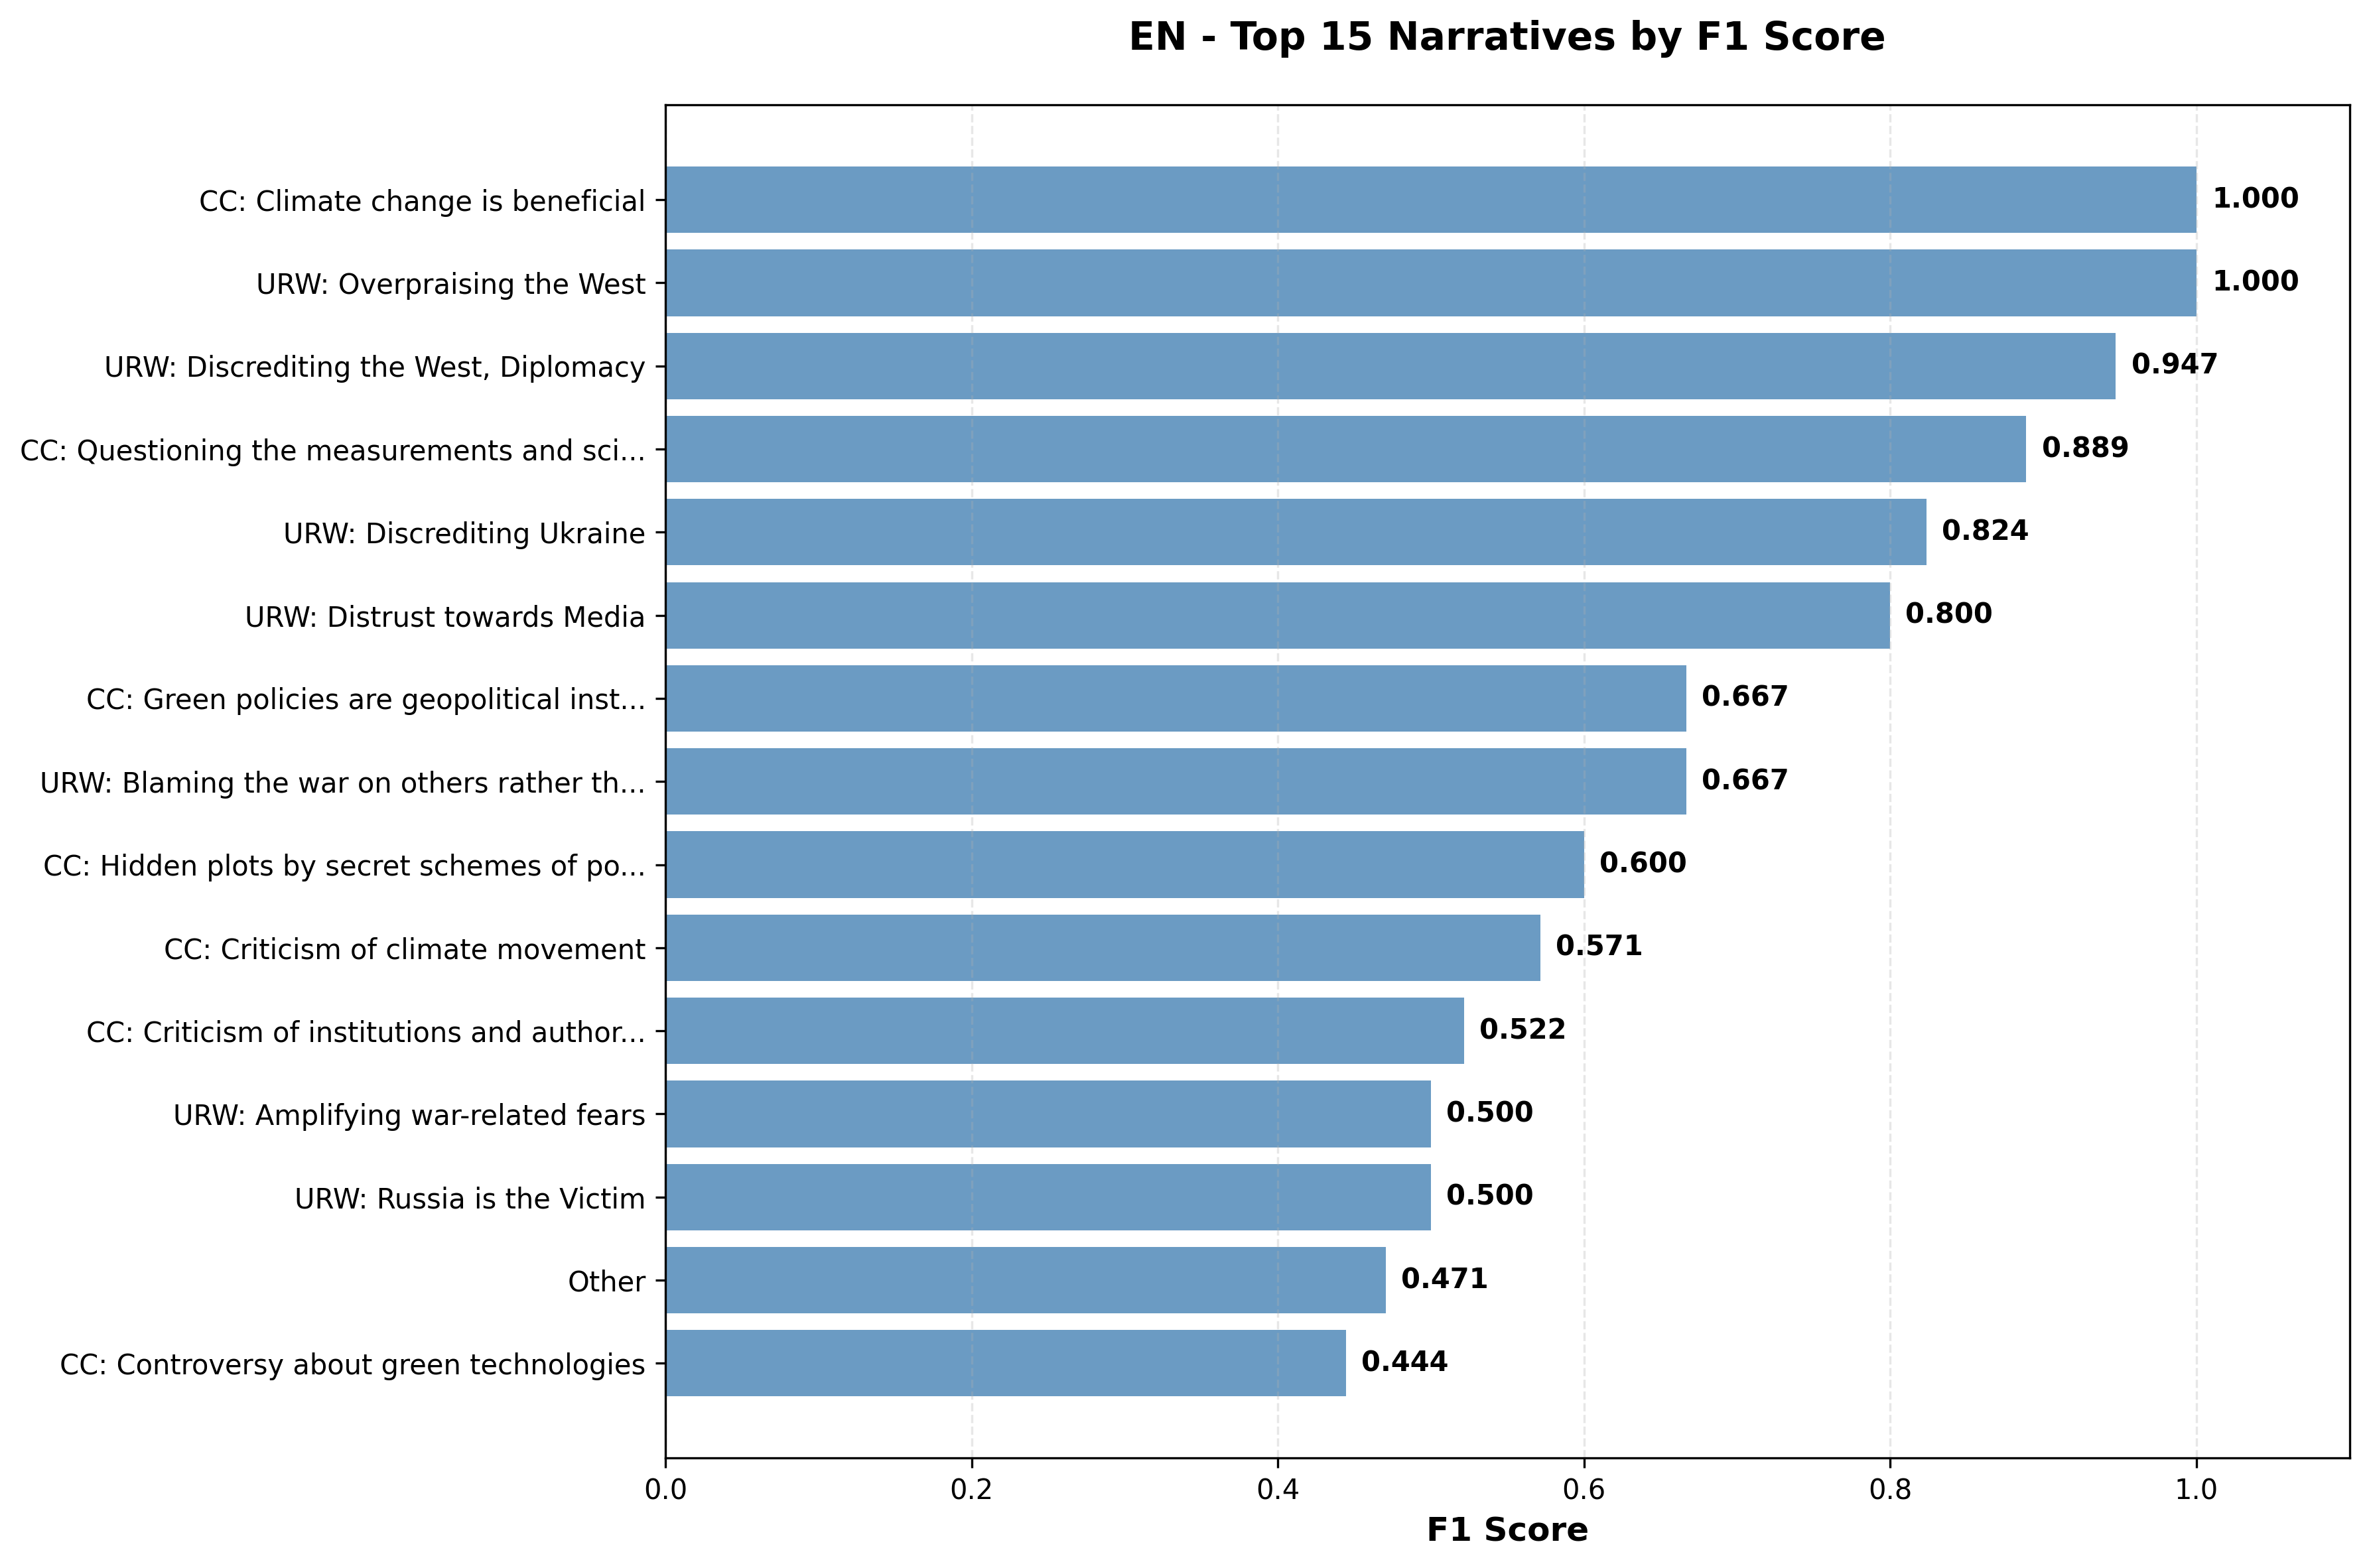
\includegraphics[width=\textwidth]{gemini25_flash_narr_val_evaluation/plots/EN_top_narratives_f1_scores.png}
        \caption{Top narrative F1 scores}
        \label{fig:app-narr-val-en-narr}
    \end{subfigure}
    \hfill
    \begin{subfigure}[b]{0.48\textwidth}
        \centering
        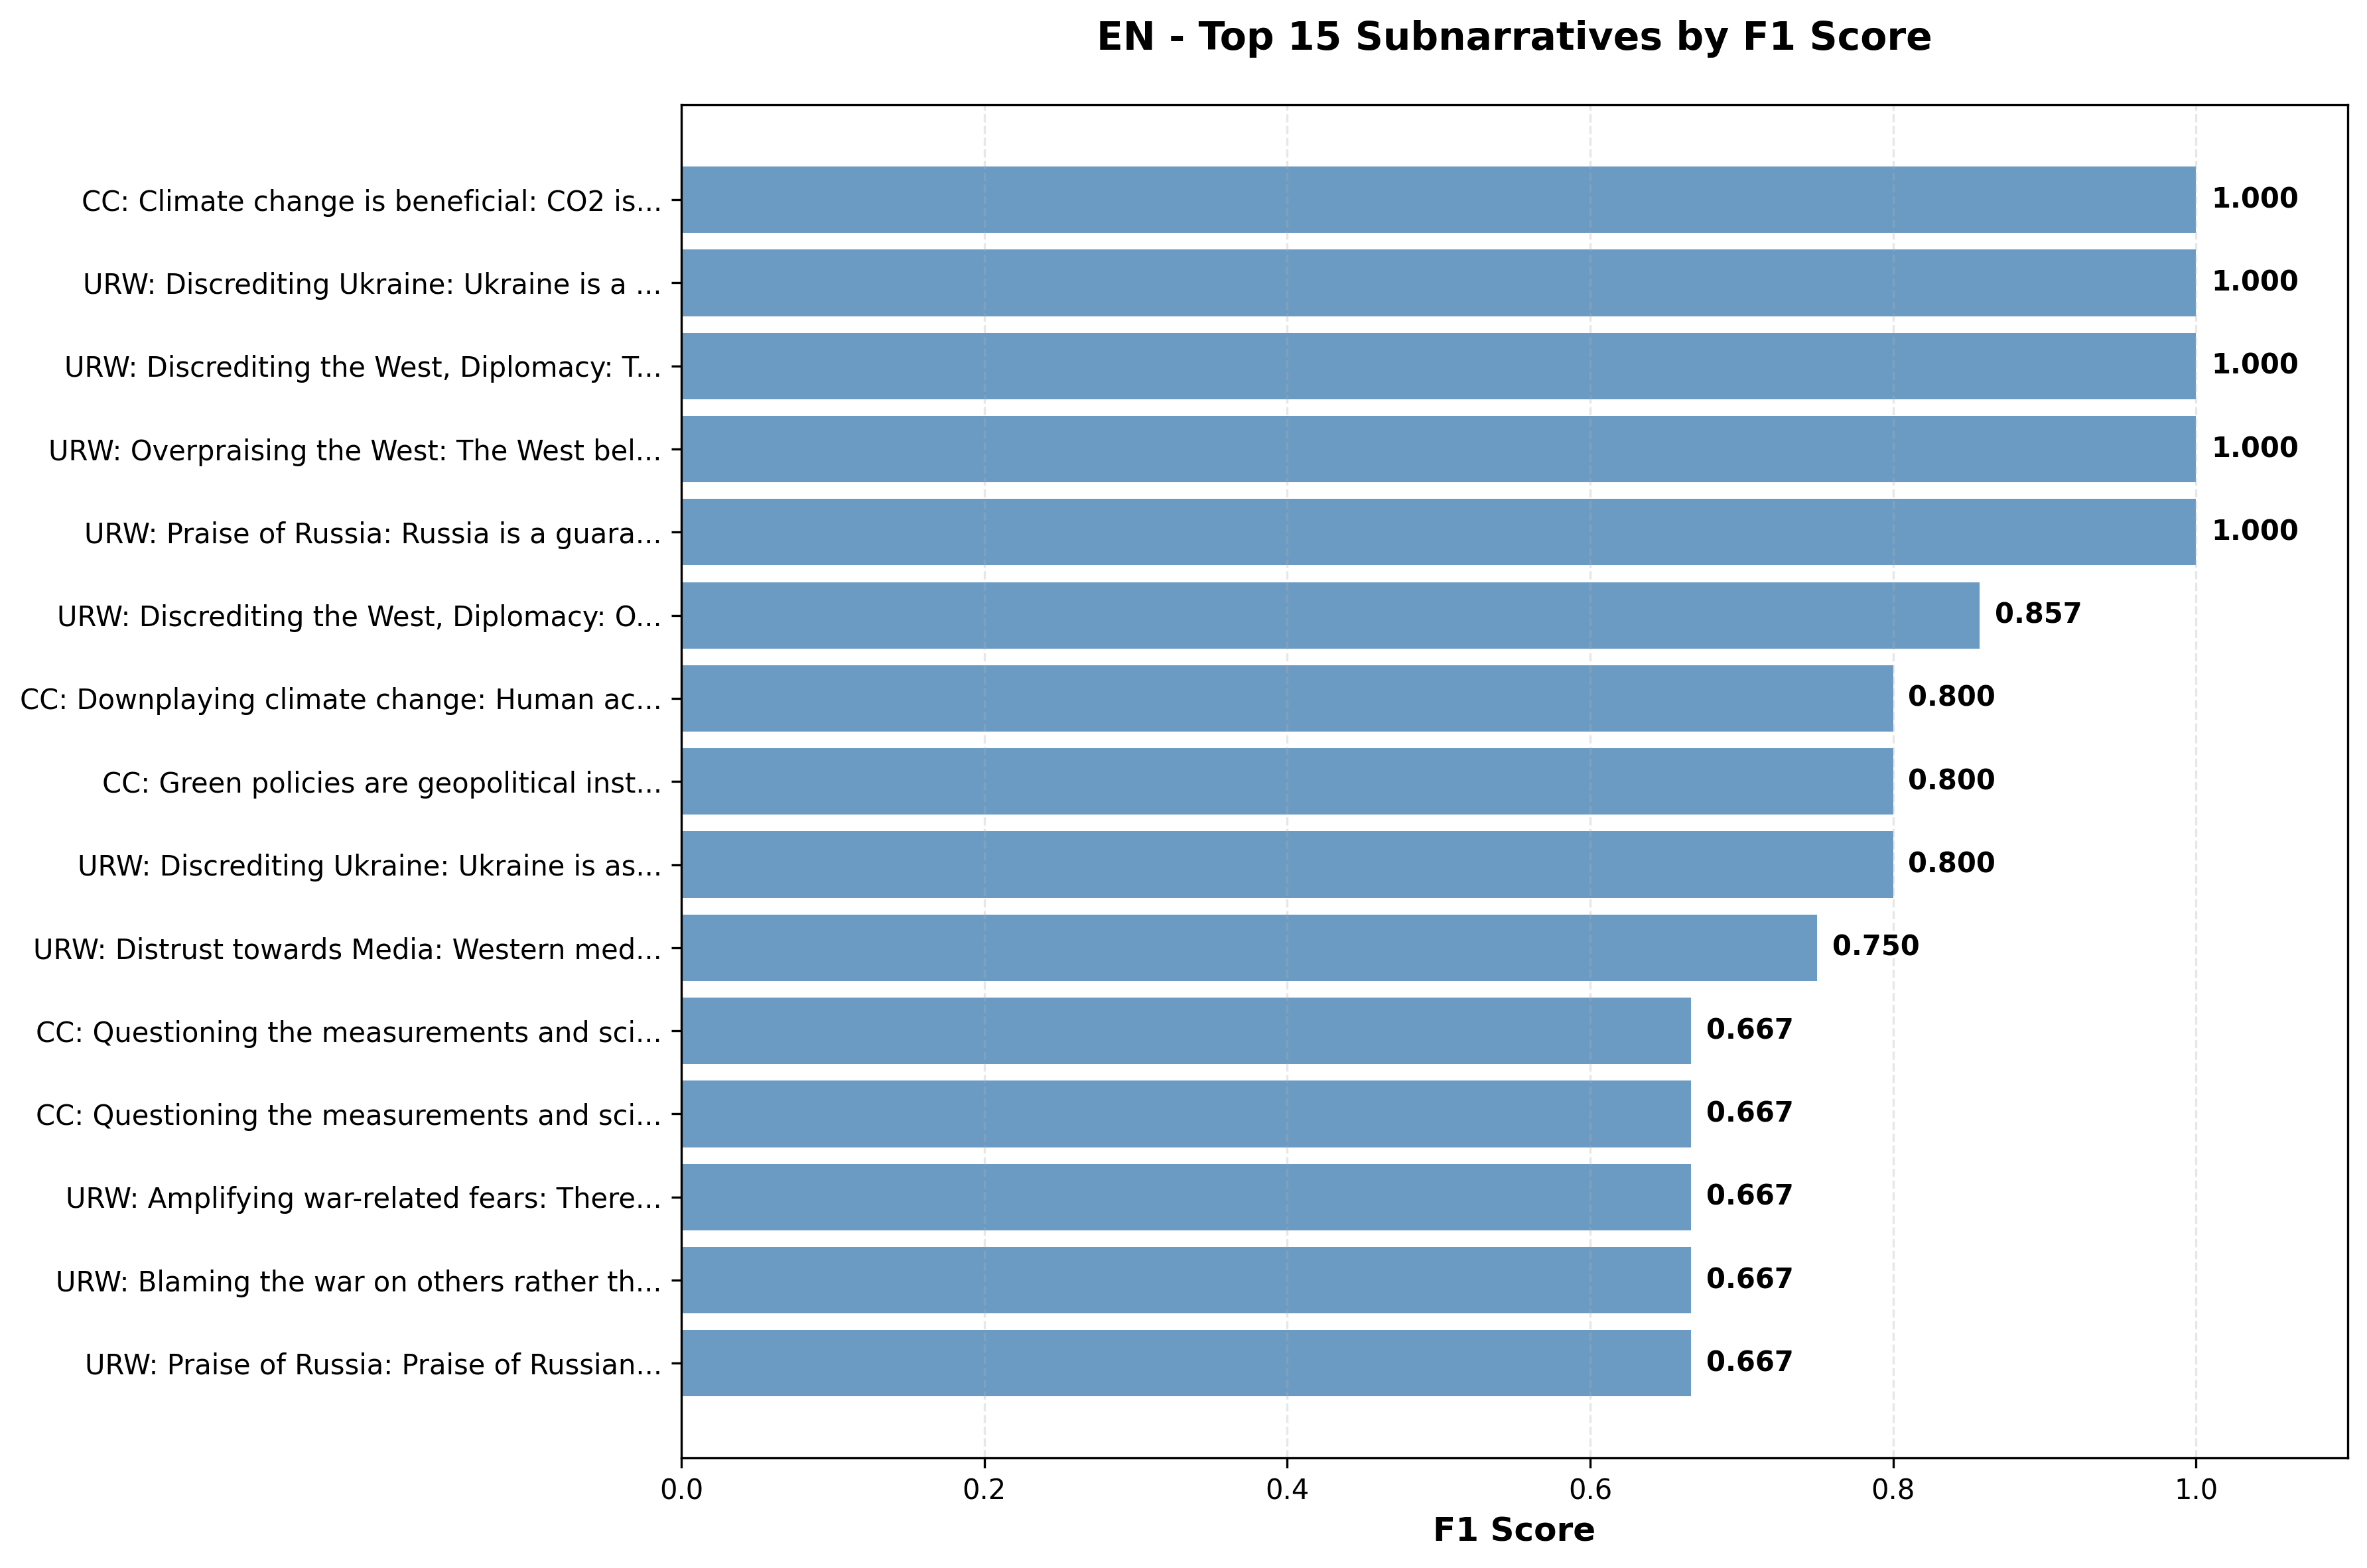
\includegraphics[width=\textwidth]{gemini25_flash_narr_val_evaluation/plots/EN_top_subnarratives_f1_scores.png}
        \caption{Top subnarrative F1 scores}
        \label{fig:app-narr-val-en-subnarr}
    \end{subfigure}
    \caption{English performance breakdown for narrative-validation configuration.}
    \label{fig:app-narr-val-en}
\end{figure}

\subsection{Hindi (HI) Performance}

\begin{figure}[H]
    \centering
    \begin{subfigure}[b]{0.48\textwidth}
        \centering
        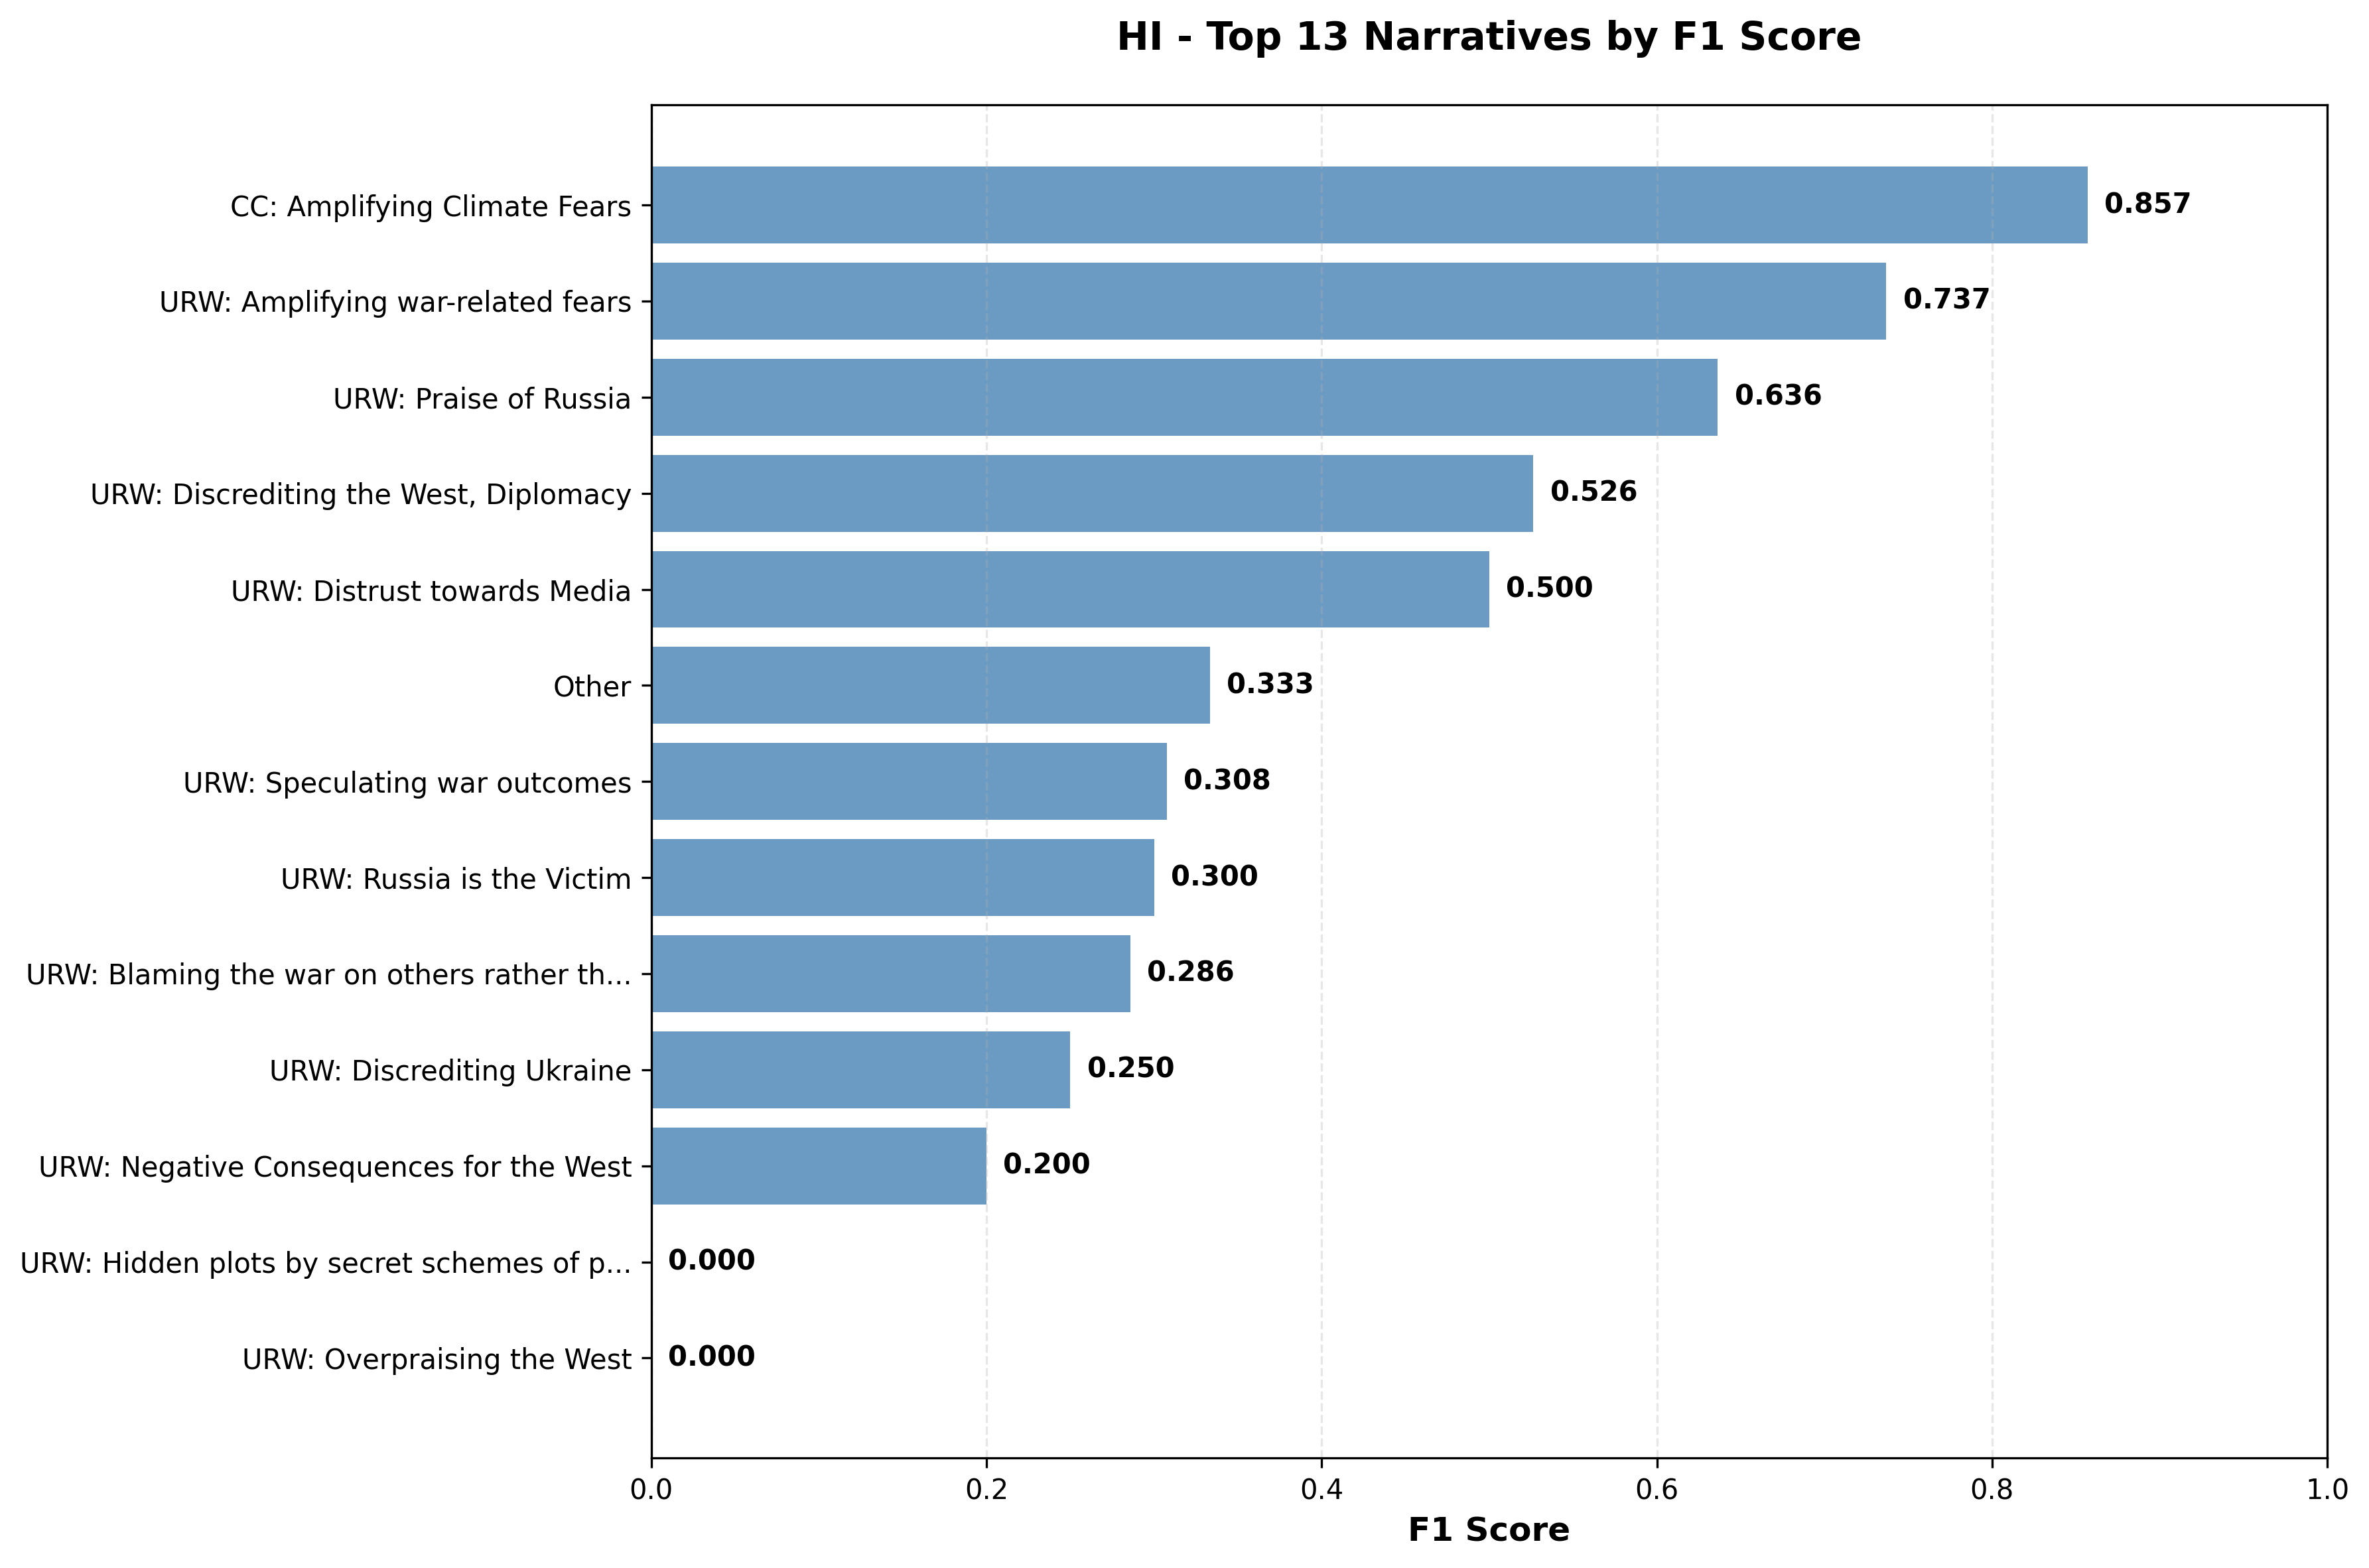
\includegraphics[width=\textwidth]{gemini25_flash_narr_val_evaluation/plots/HI_top_narratives_f1_scores.png}
        \caption{Top narrative F1 scores}
        \label{fig:app-narr-val-hi-narr}
    \end{subfigure}
    \hfill
    \begin{subfigure}[b]{0.48\textwidth}
        \centering
        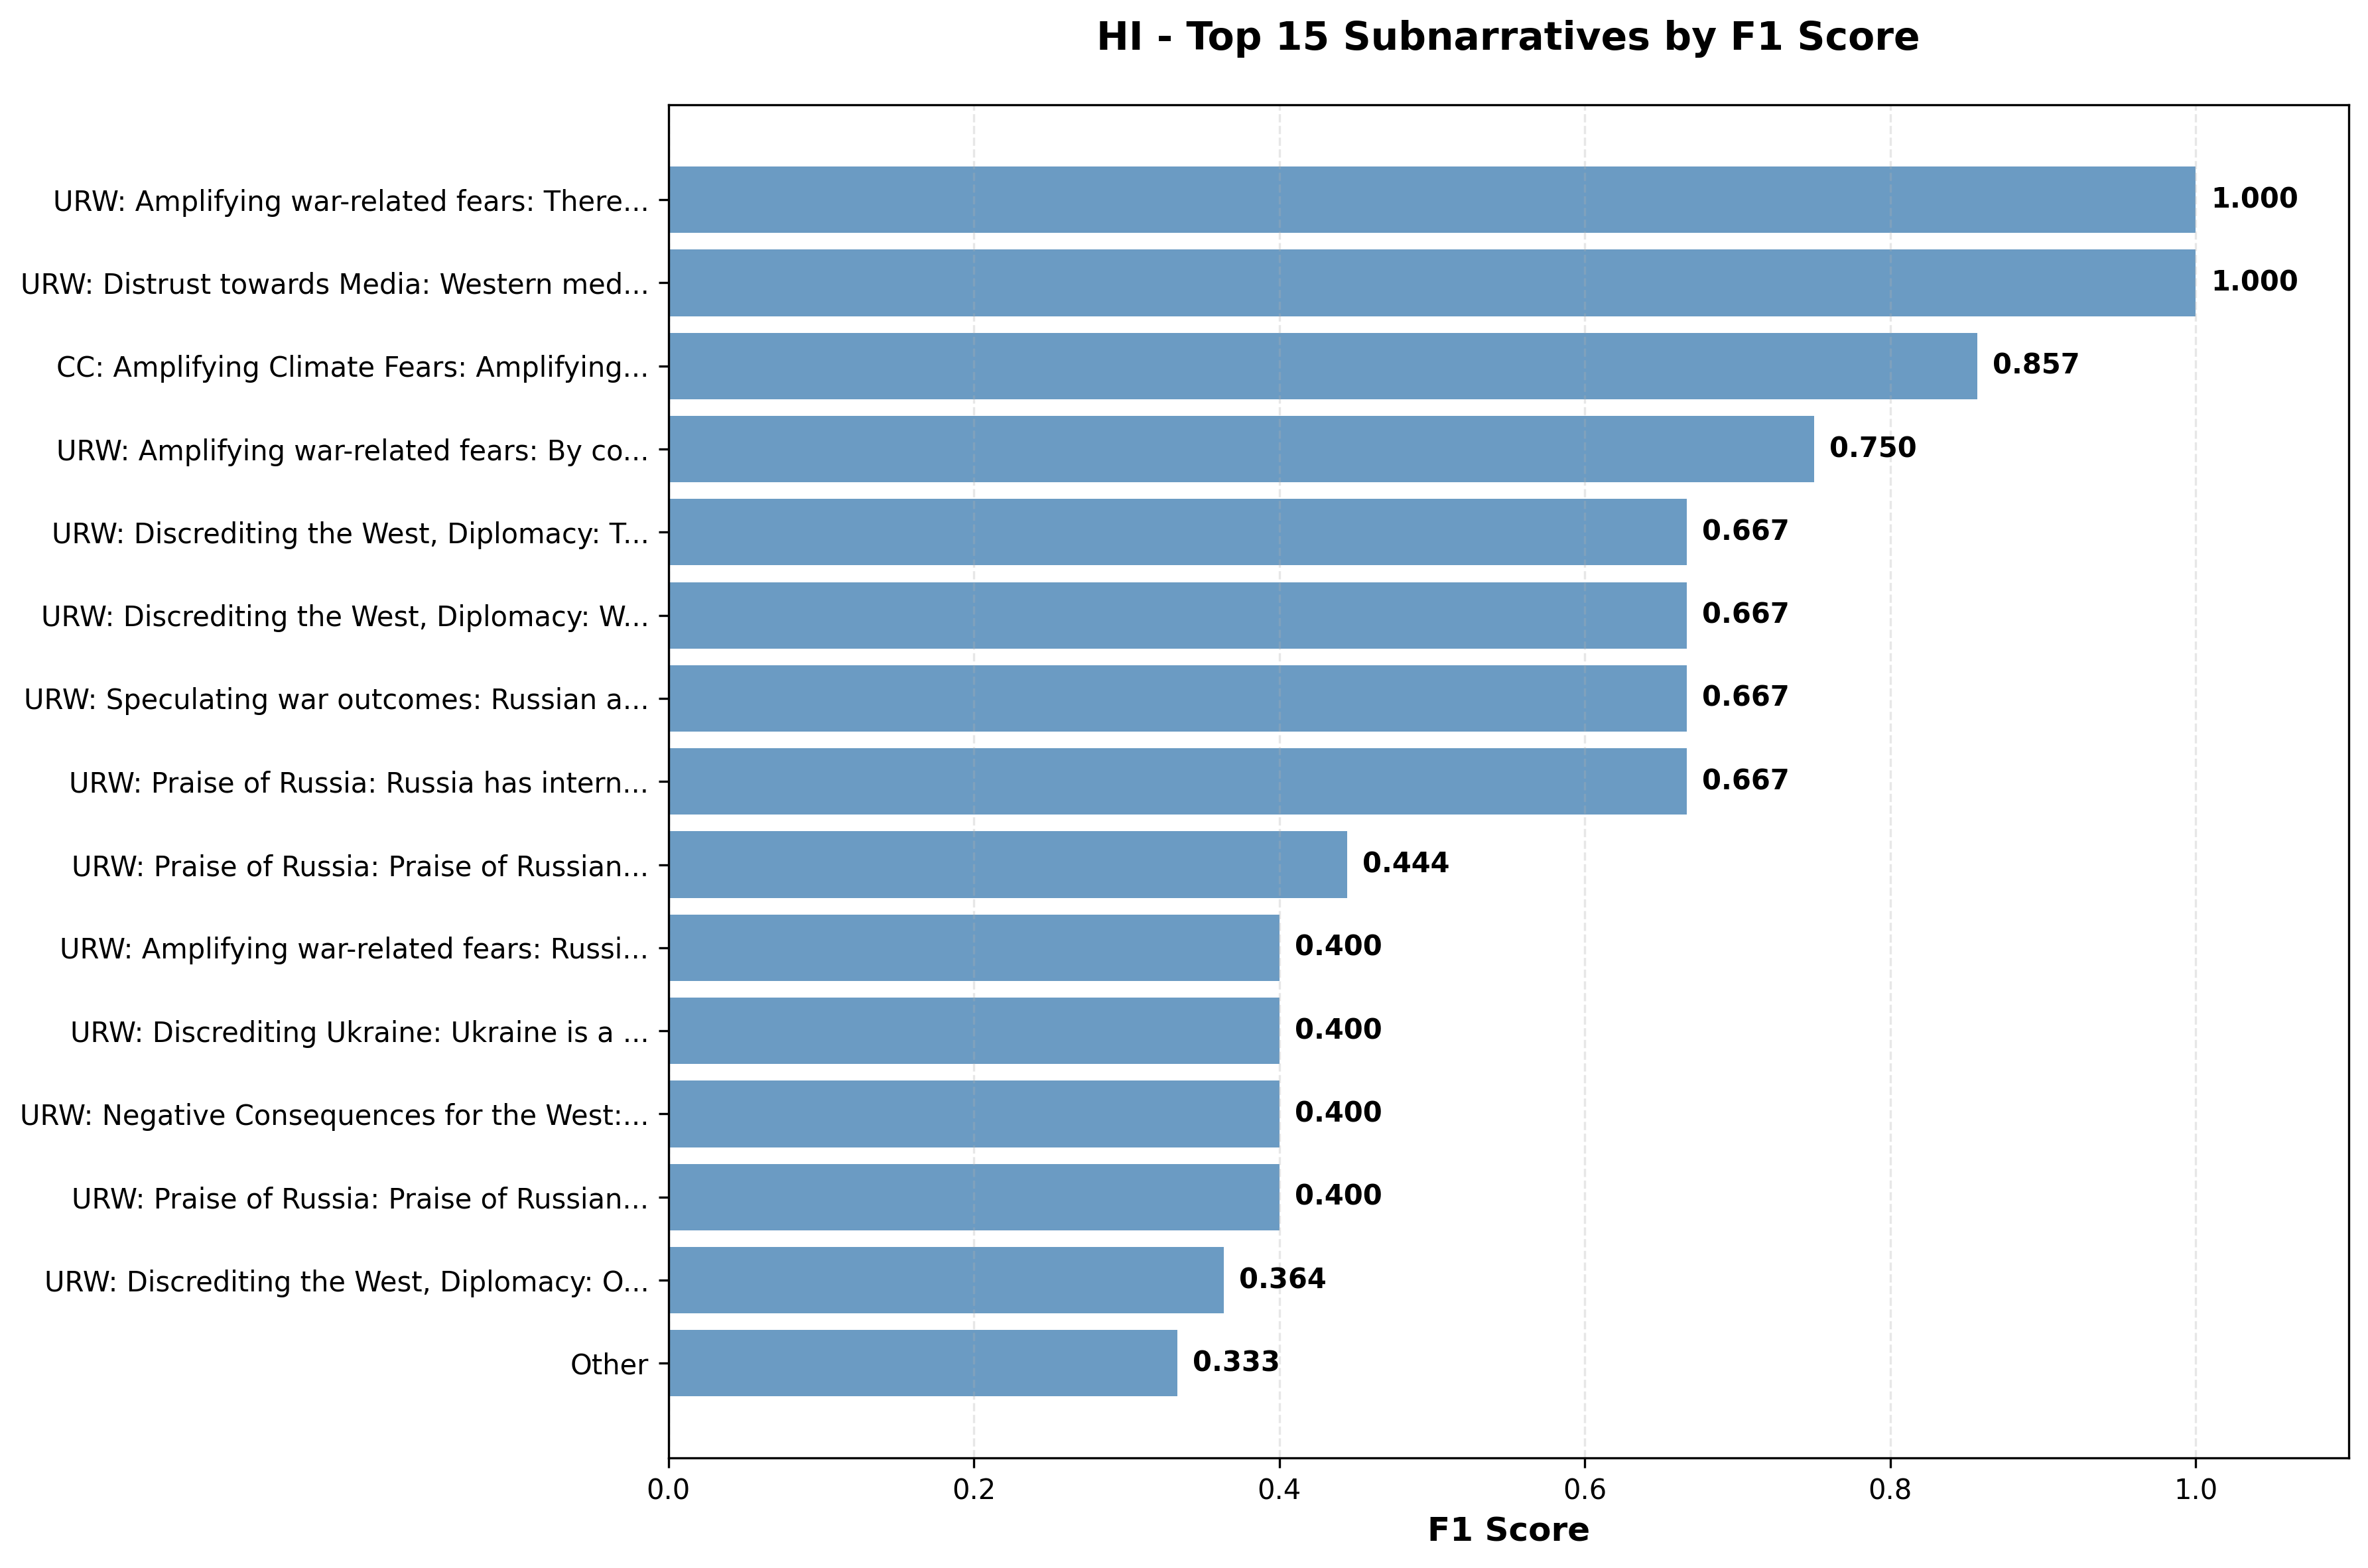
\includegraphics[width=\textwidth]{gemini25_flash_narr_val_evaluation/plots/HI_top_subnarratives_f1_scores.png}
        \caption{Top subnarrative F1 scores}
        \label{fig:app-narr-val-hi-subnarr}
    \end{subfigure}
    \caption{Hindi performance breakdown for narrative-validation configuration.}
    \label{fig:app-narr-val-hi}
\end{figure}

\subsection{Portuguese (PT) Performance}

\begin{figure}[H]
    \centering
    \begin{subfigure}[b]{0.48\textwidth}
        \centering
        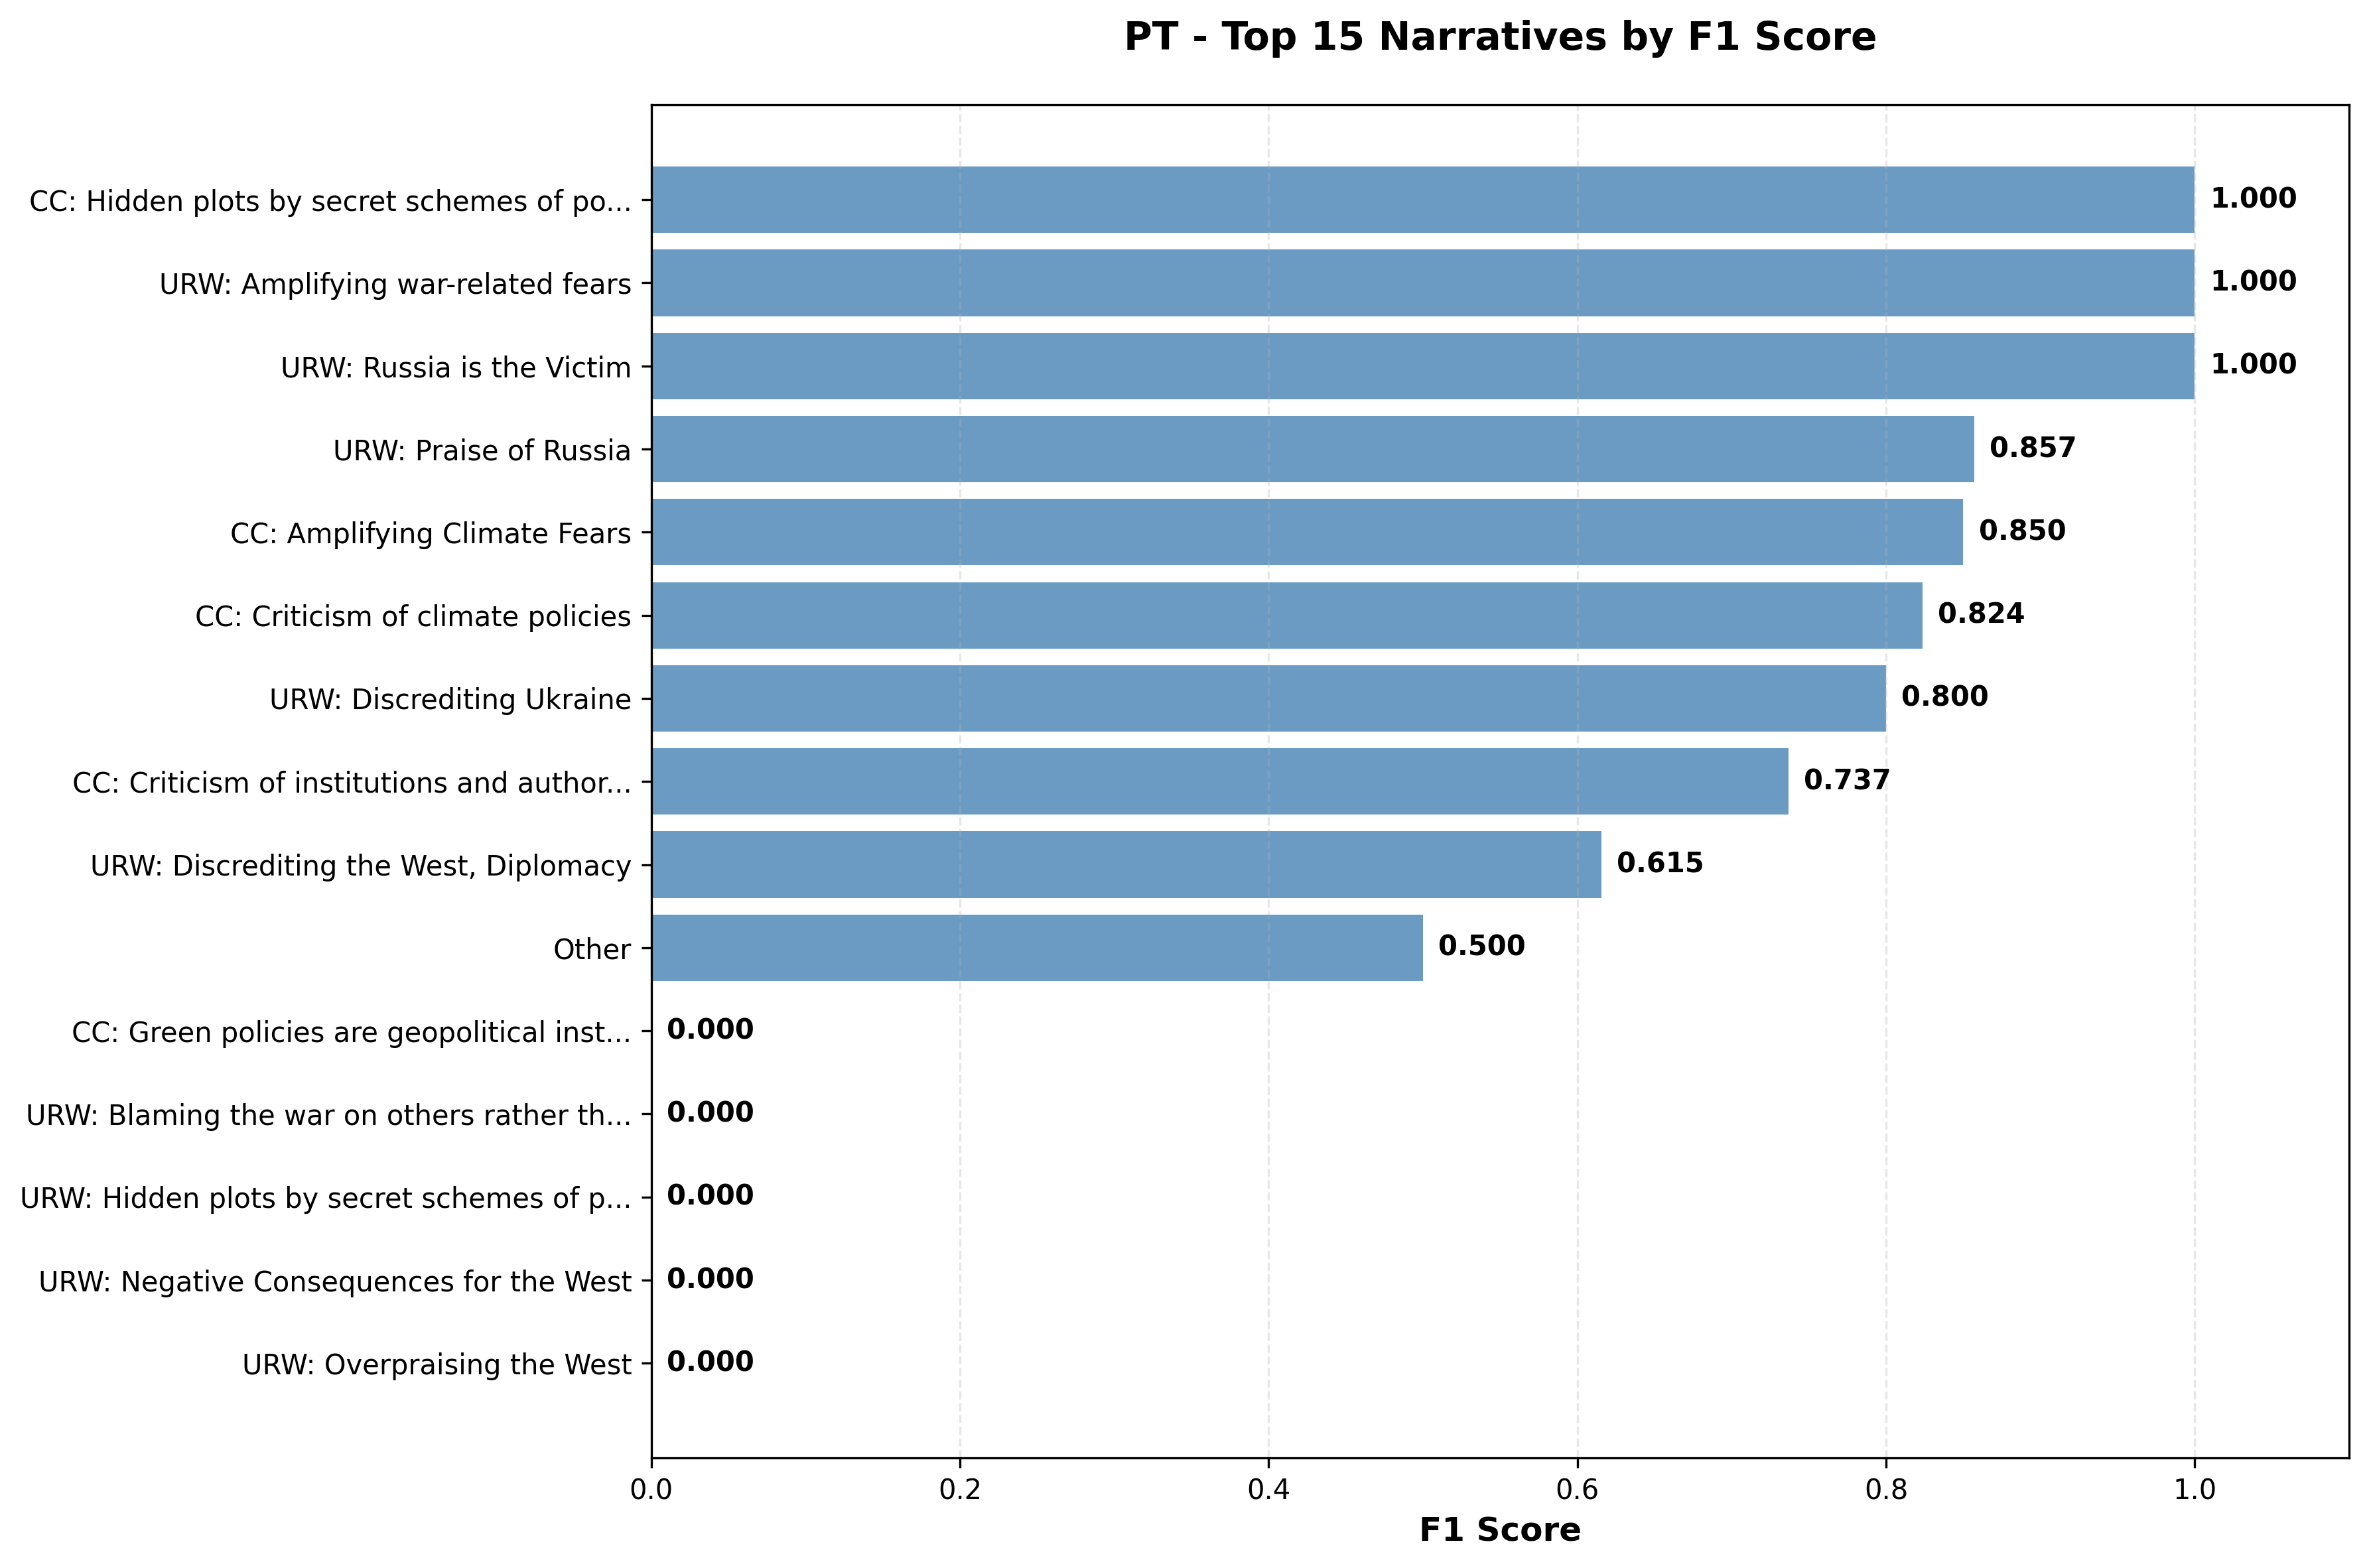
\includegraphics[width=\textwidth]{gemini25_flash_narr_val_evaluation/plots/PT_top_narratives_f1_scores.png}
        \caption{Top narrative F1 scores}
        \label{fig:app-narr-val-pt-narr}
    \end{subfigure}
    \hfill
    \begin{subfigure}[b]{0.48\textwidth}
        \centering
        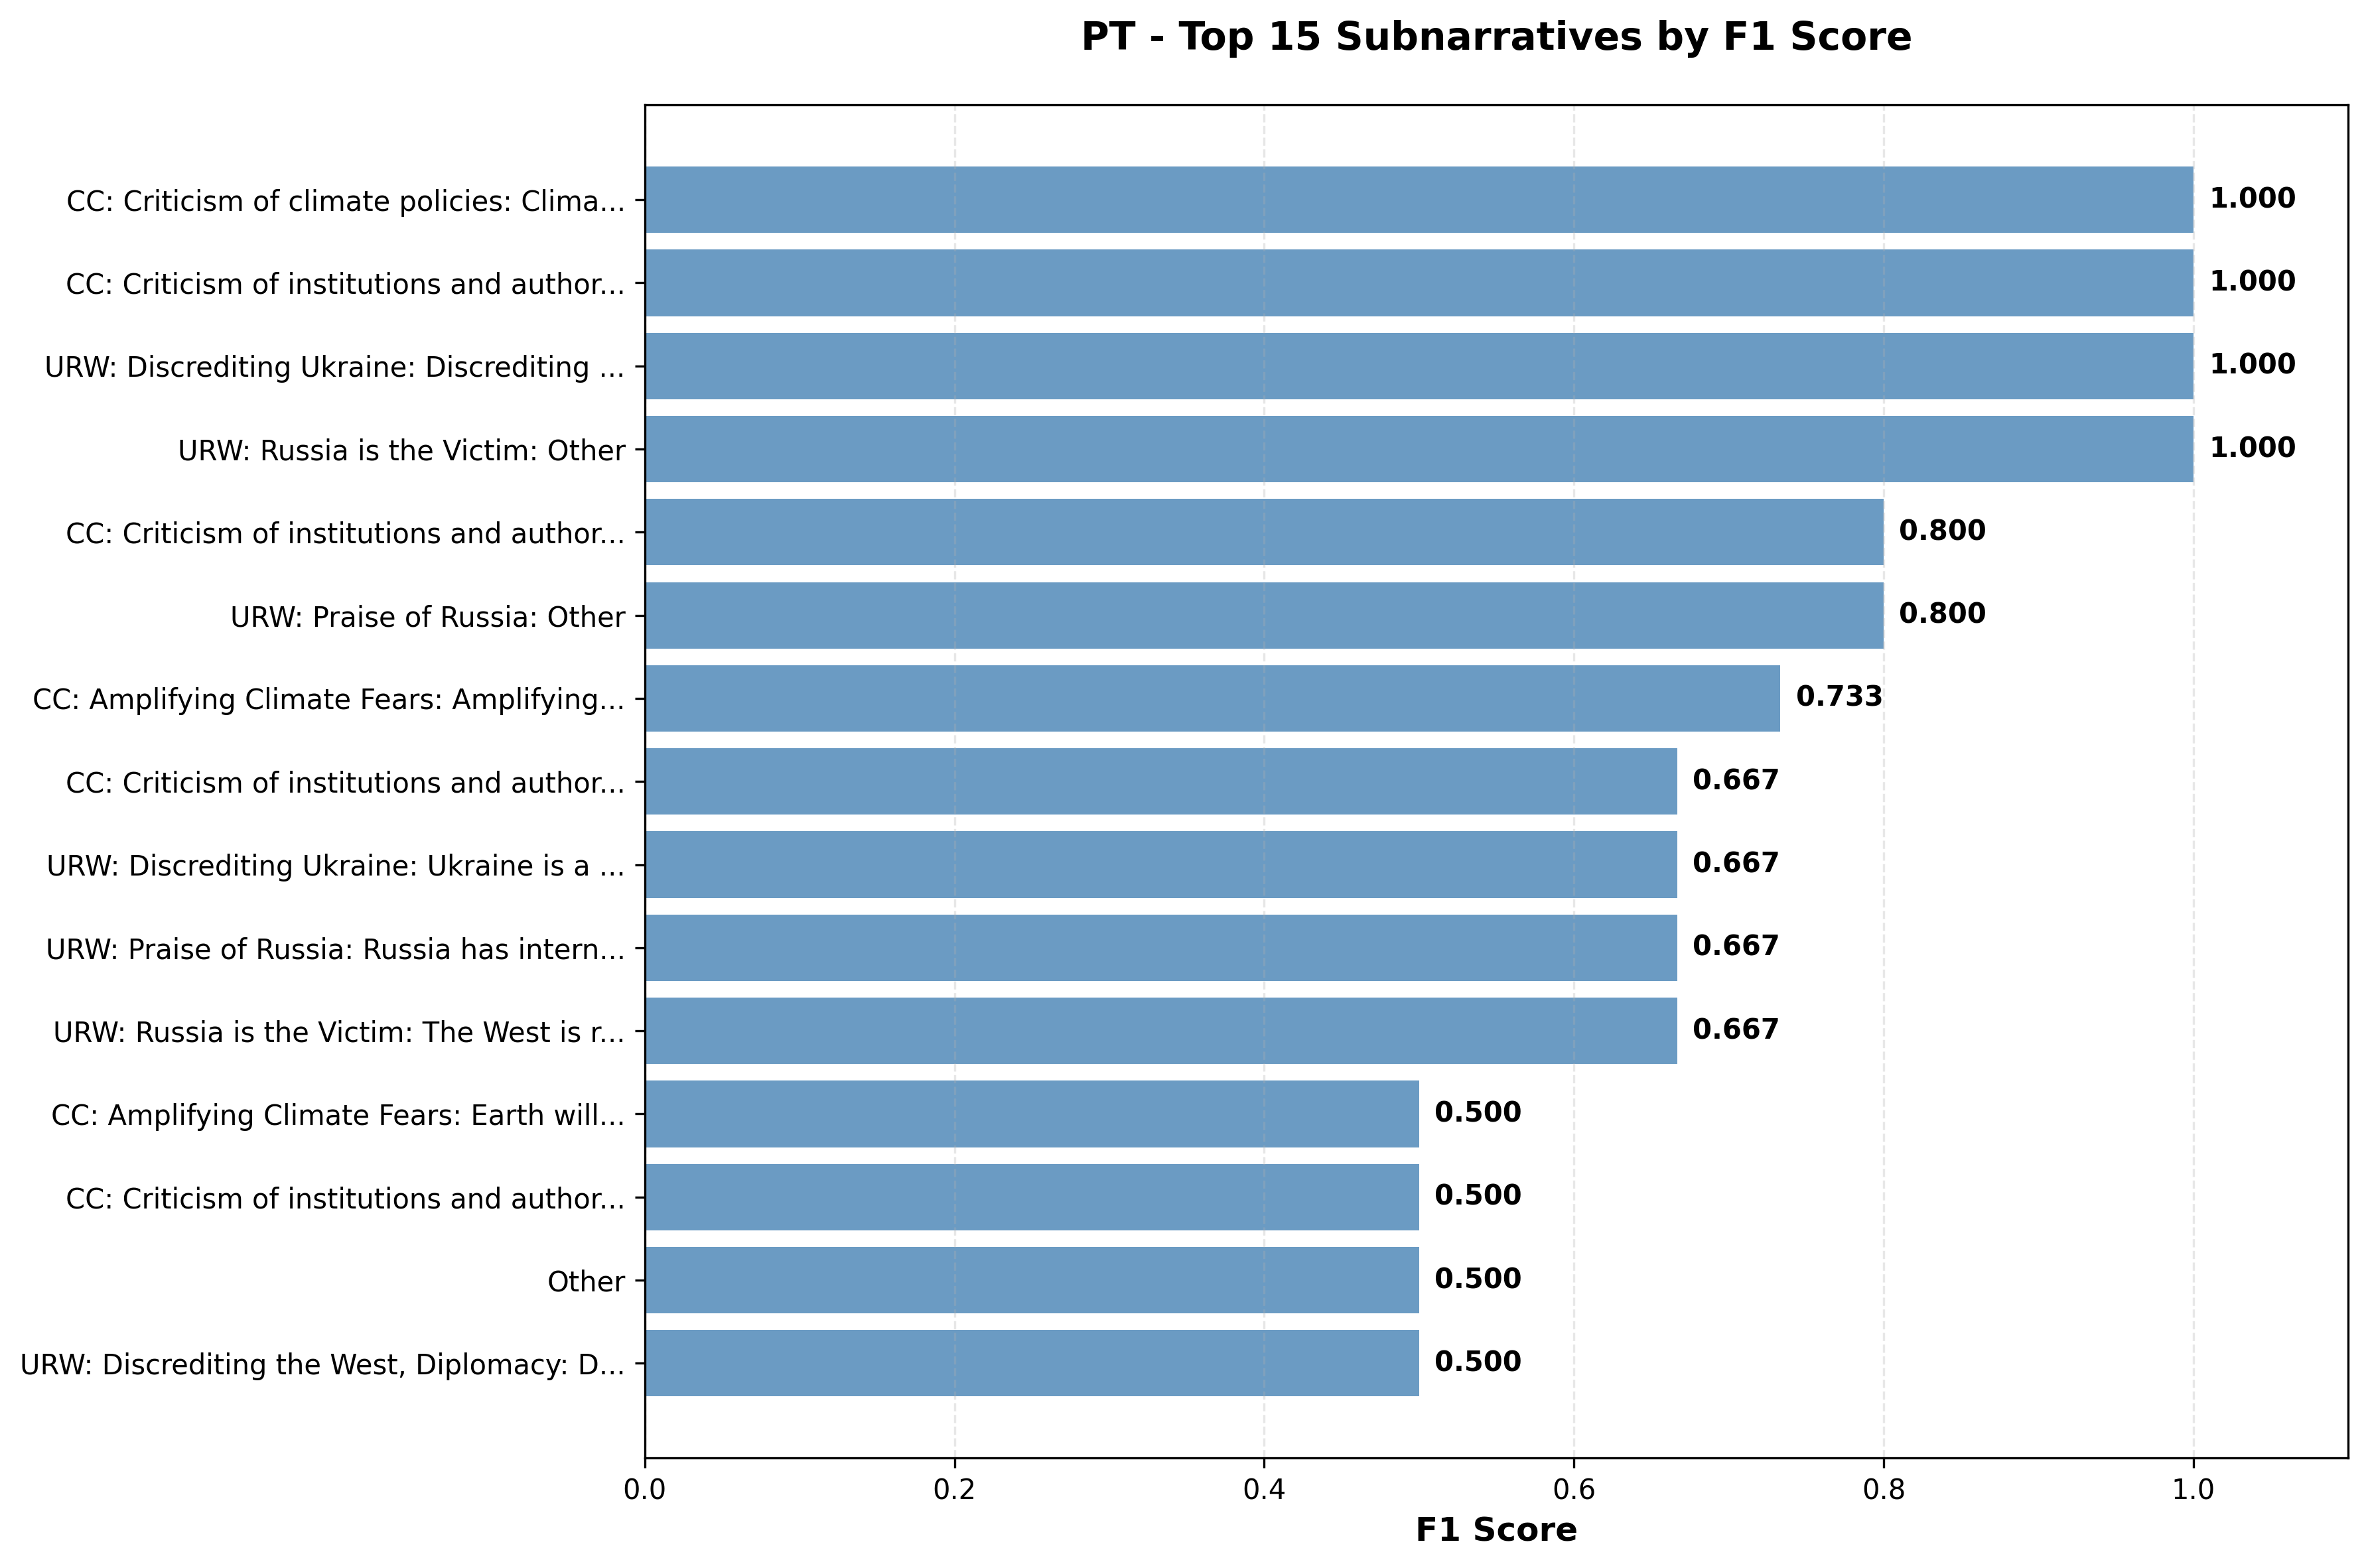
\includegraphics[width=\textwidth]{gemini25_flash_narr_val_evaluation/plots/PT_top_subnarratives_f1_scores.png}
        \caption{Top subnarrative F1 scores}
        \label{fig:app-narr-val-pt-subnarr}
    \end{subfigure}
    \caption{Portuguese performance breakdown for narrative-validation configuration.}
    \label{fig:app-narr-val-pt}
\end{figure}

\subsection{Russian (RU) Performance}

\begin{figure}[H]
    \centering
    \begin{subfigure}[b]{0.48\textwidth}
        \centering
        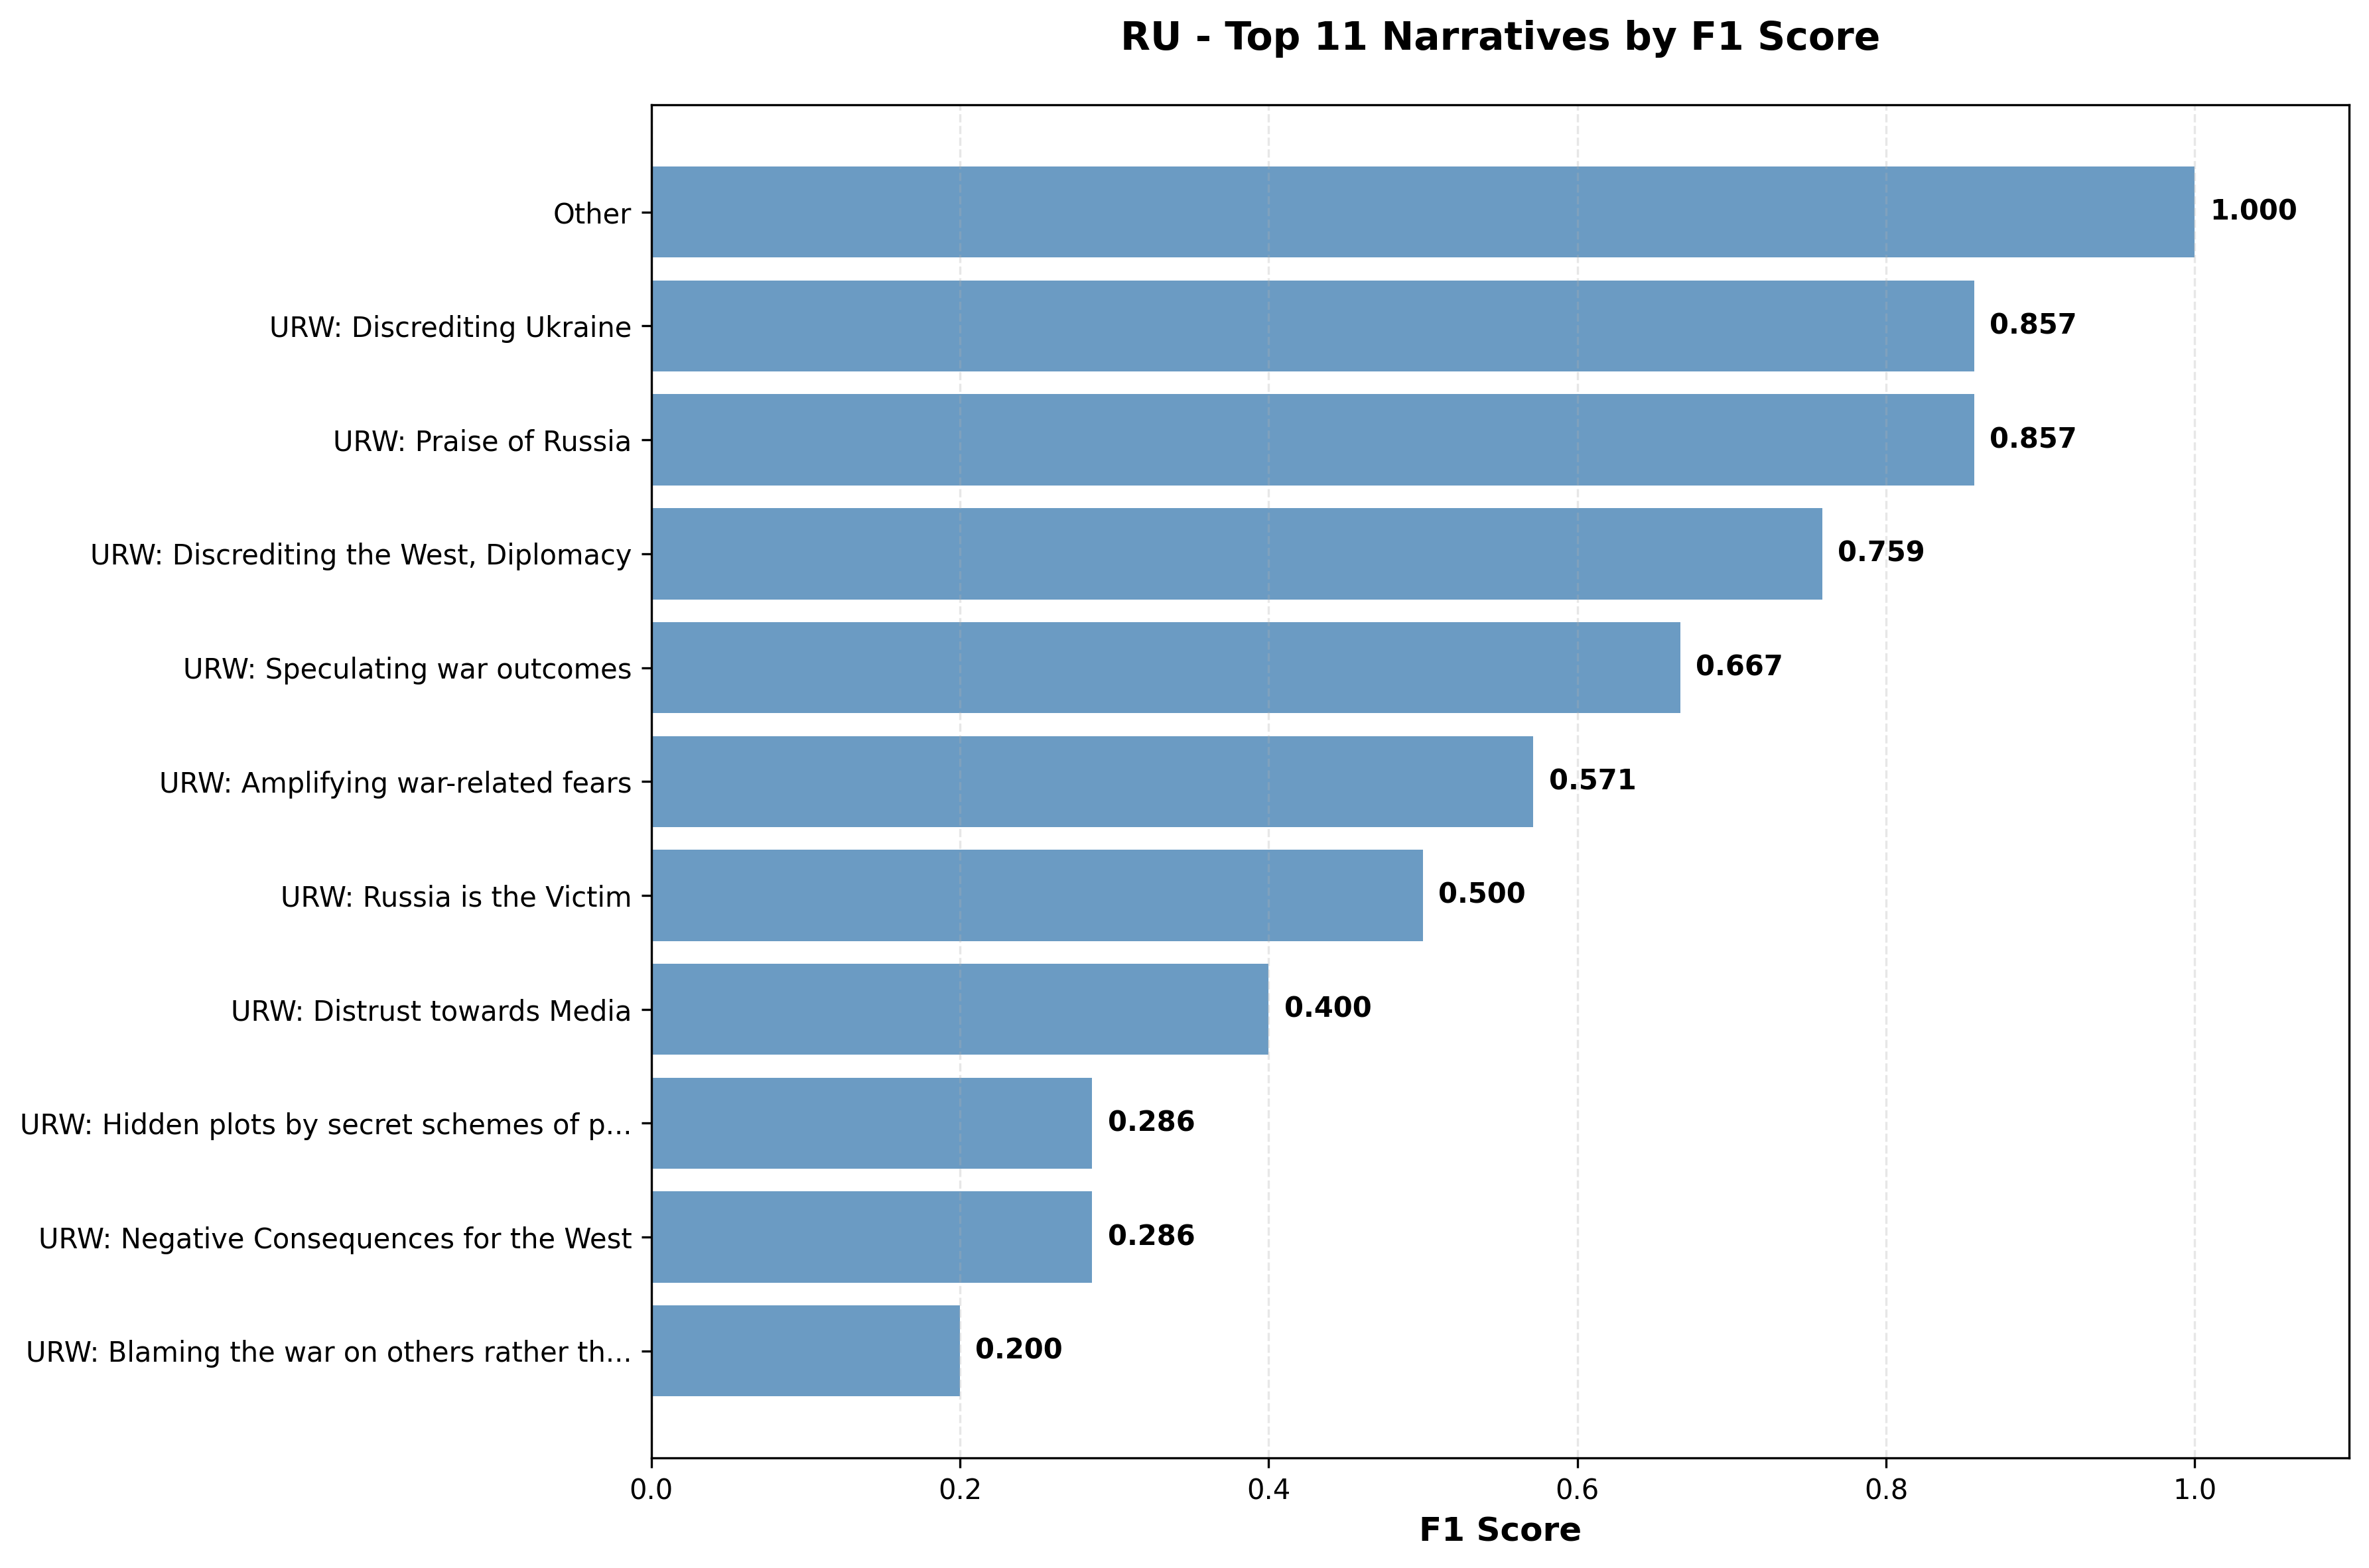
\includegraphics[width=\textwidth]{gemini25_flash_narr_val_evaluation/plots/RU_top_narratives_f1_scores.png}
        \caption{Top narrative F1 scores}
        \label{fig:app-narr-val-ru-narr}
    \end{subfigure}
    \hfill
    \begin{subfigure}[b]{0.48\textwidth}
        \centering
        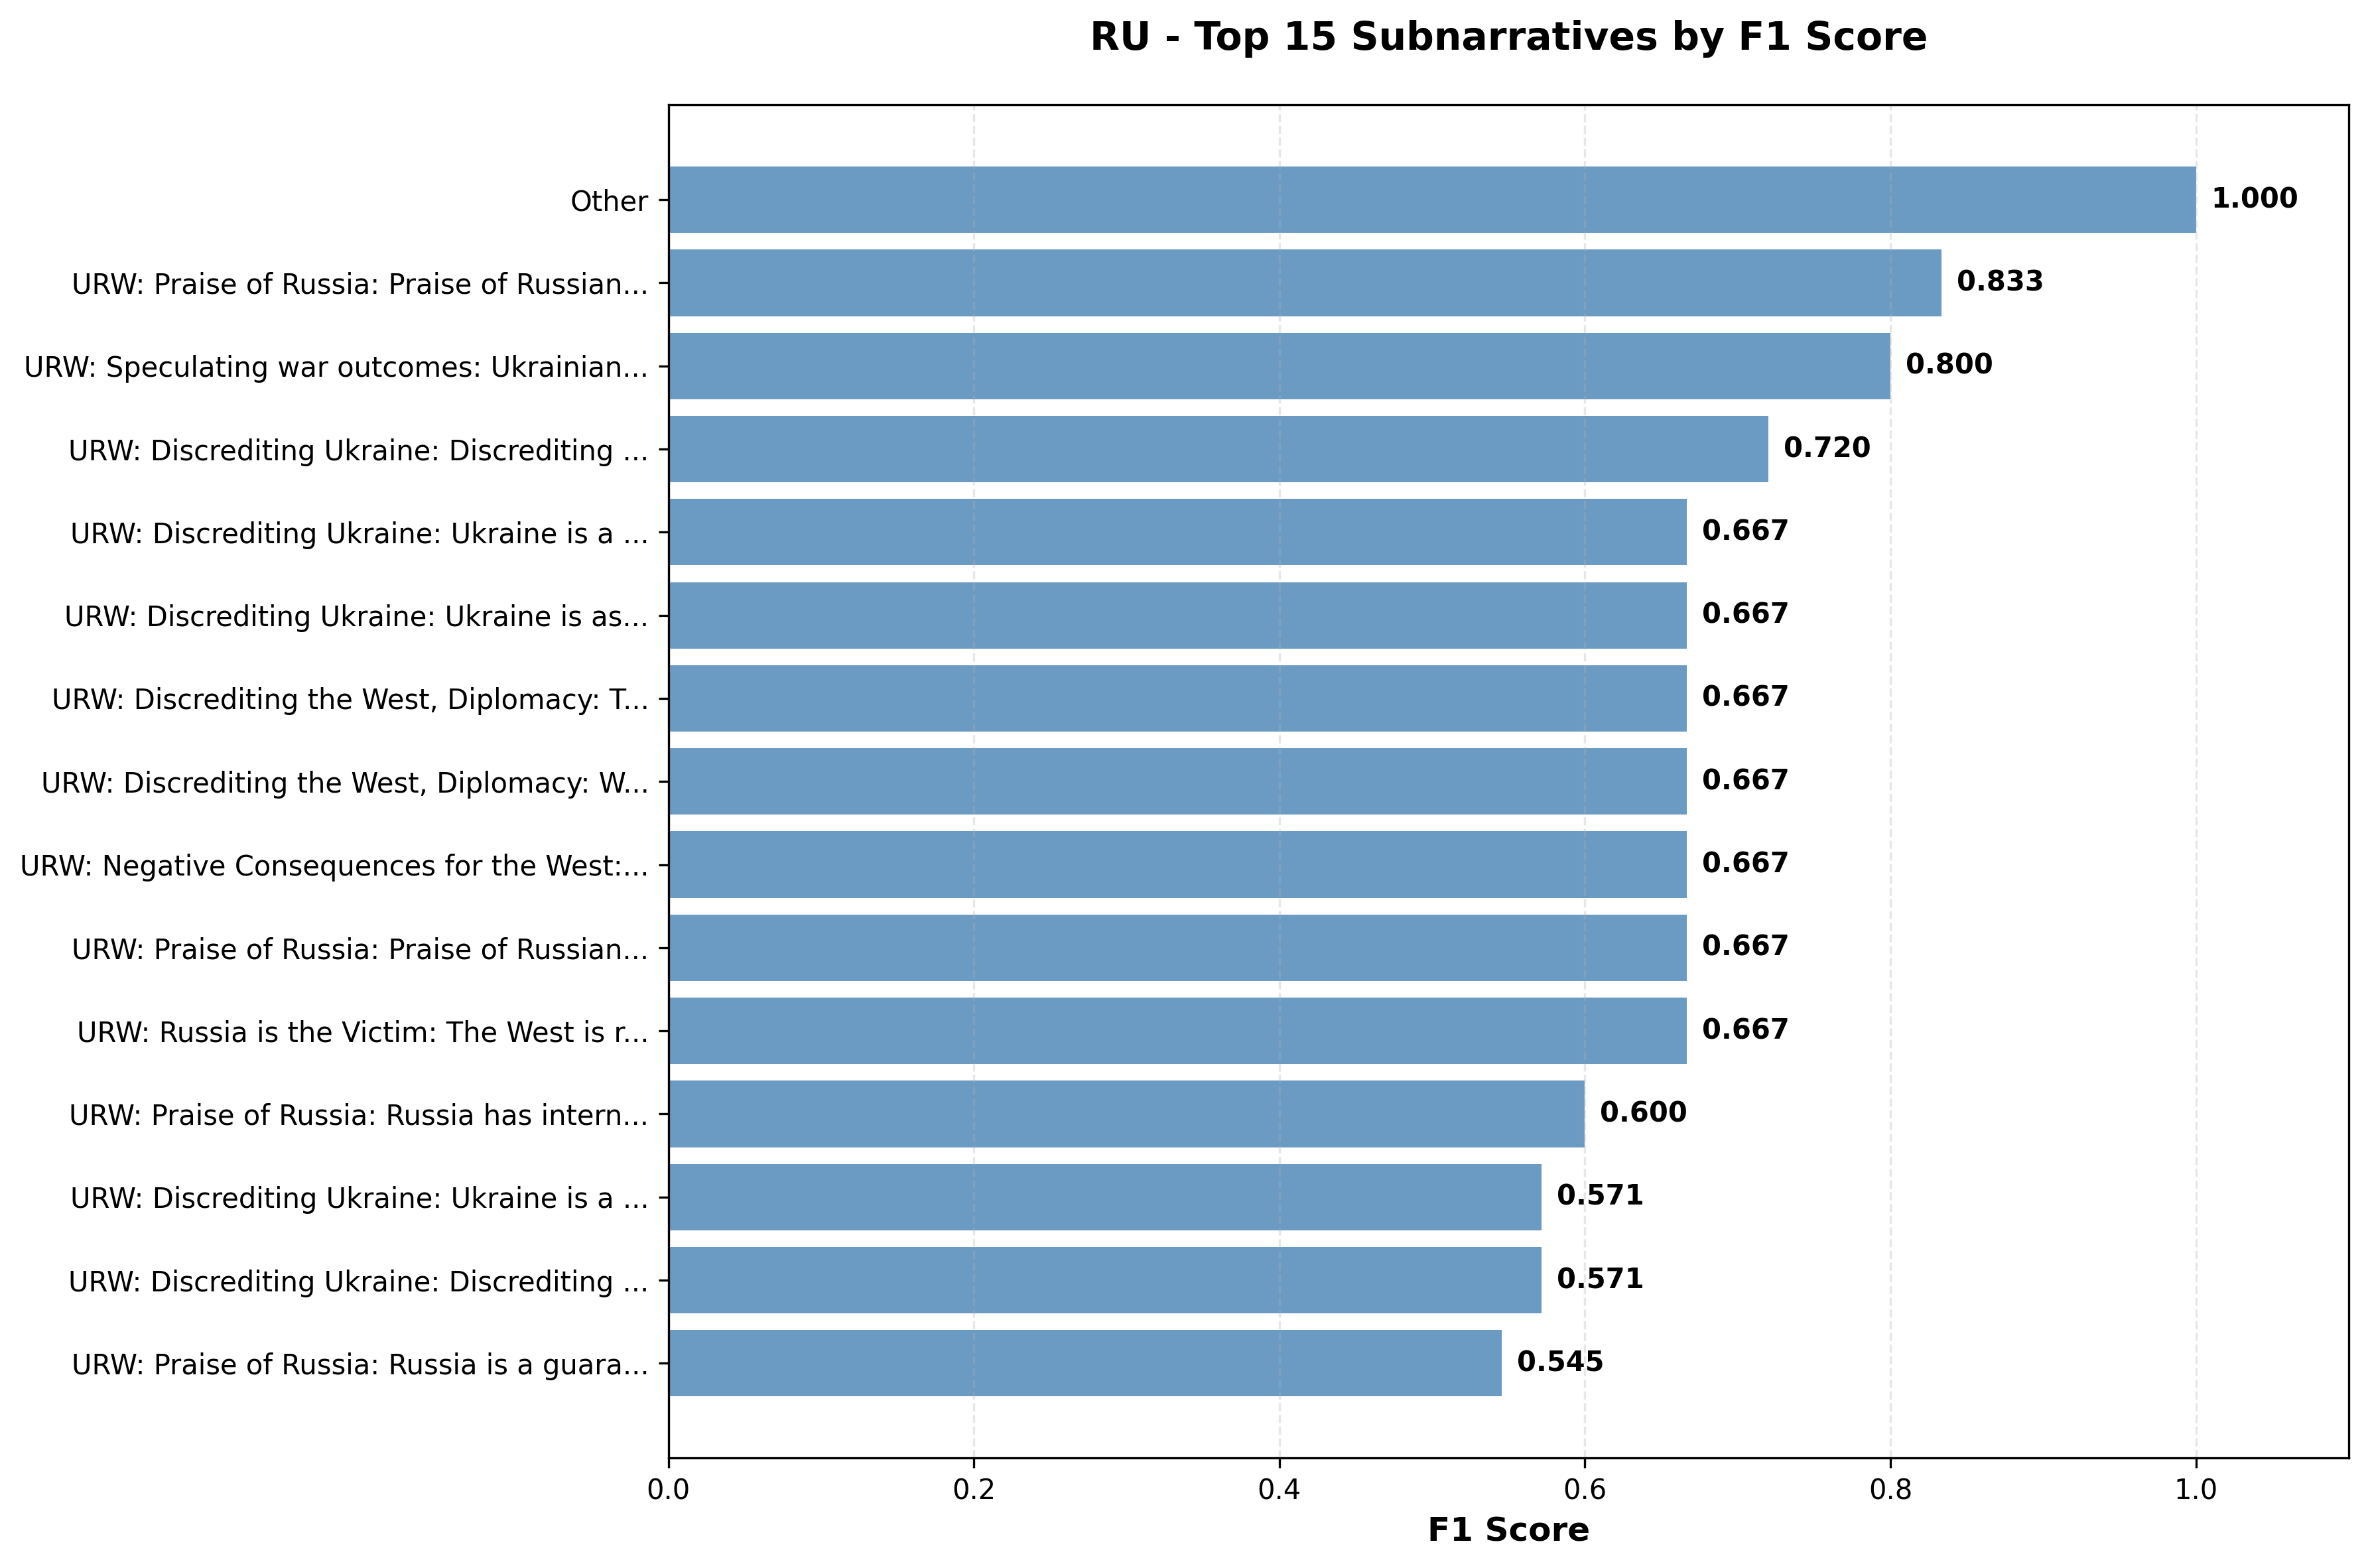
\includegraphics[width=\textwidth]{gemini25_flash_narr_val_evaluation/plots/RU_top_subnarratives_f1_scores.png}
        \caption{Top subnarrative F1 scores}
        \label{fig:app-narr-val-ru-subnarr}
    \end{subfigure}
    \caption{Russian performance breakdown for narrative-validation configuration.}
    \label{fig:app-narr-val-ru}
\end{figure}

\clearpage
\section{Architecture 2: Subnarrative Validation Configuration}
\label{app:subnarr-validation}

This section presents results from the Actor-Critique pipeline with subnarrative-level validation enabled.

\subsection{Overall Performance Comparison}

\begin{figure}[H]
    \centering
    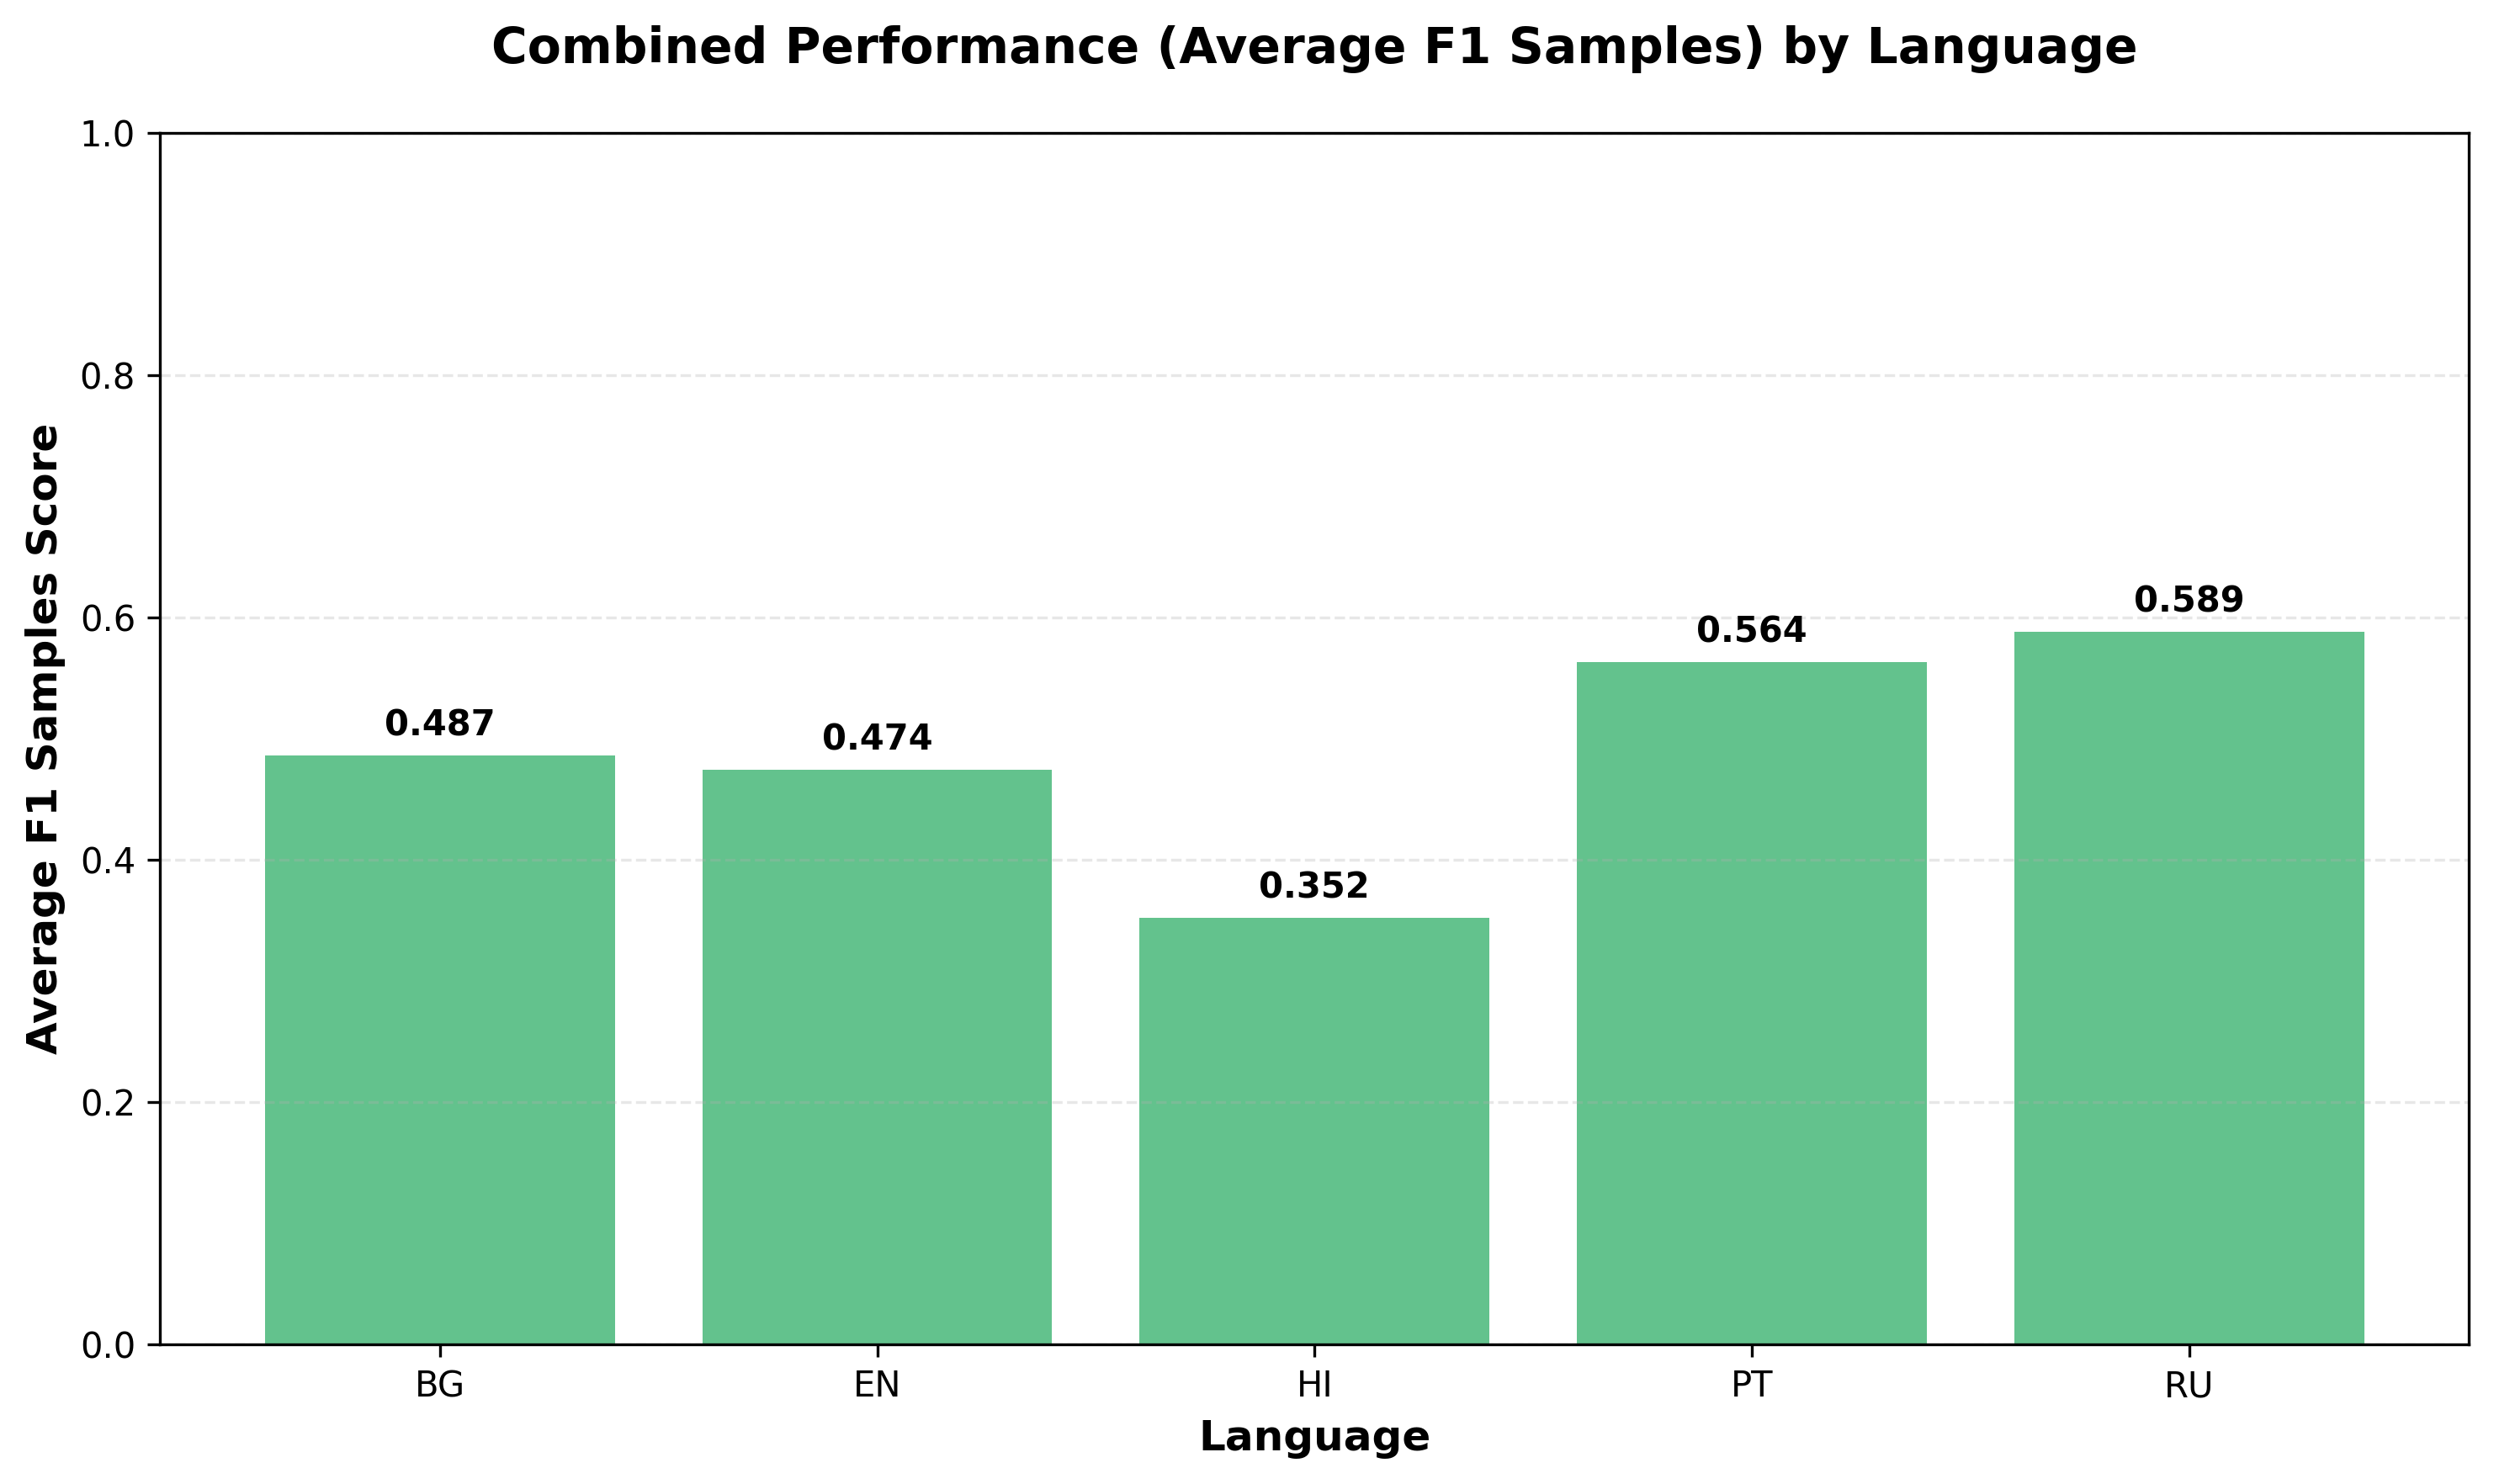
\includegraphics[width=0.85\textwidth]{gemini25_flash_subnarr_val_evaluation/plots/combined_performance_by_language.png}
    \caption{Combined performance across all languages for the subnarrative-validation configuration.}
    \label{fig:app-subnarr-val-combined}
\end{figure}

\begin{figure}[H]
    \centering
    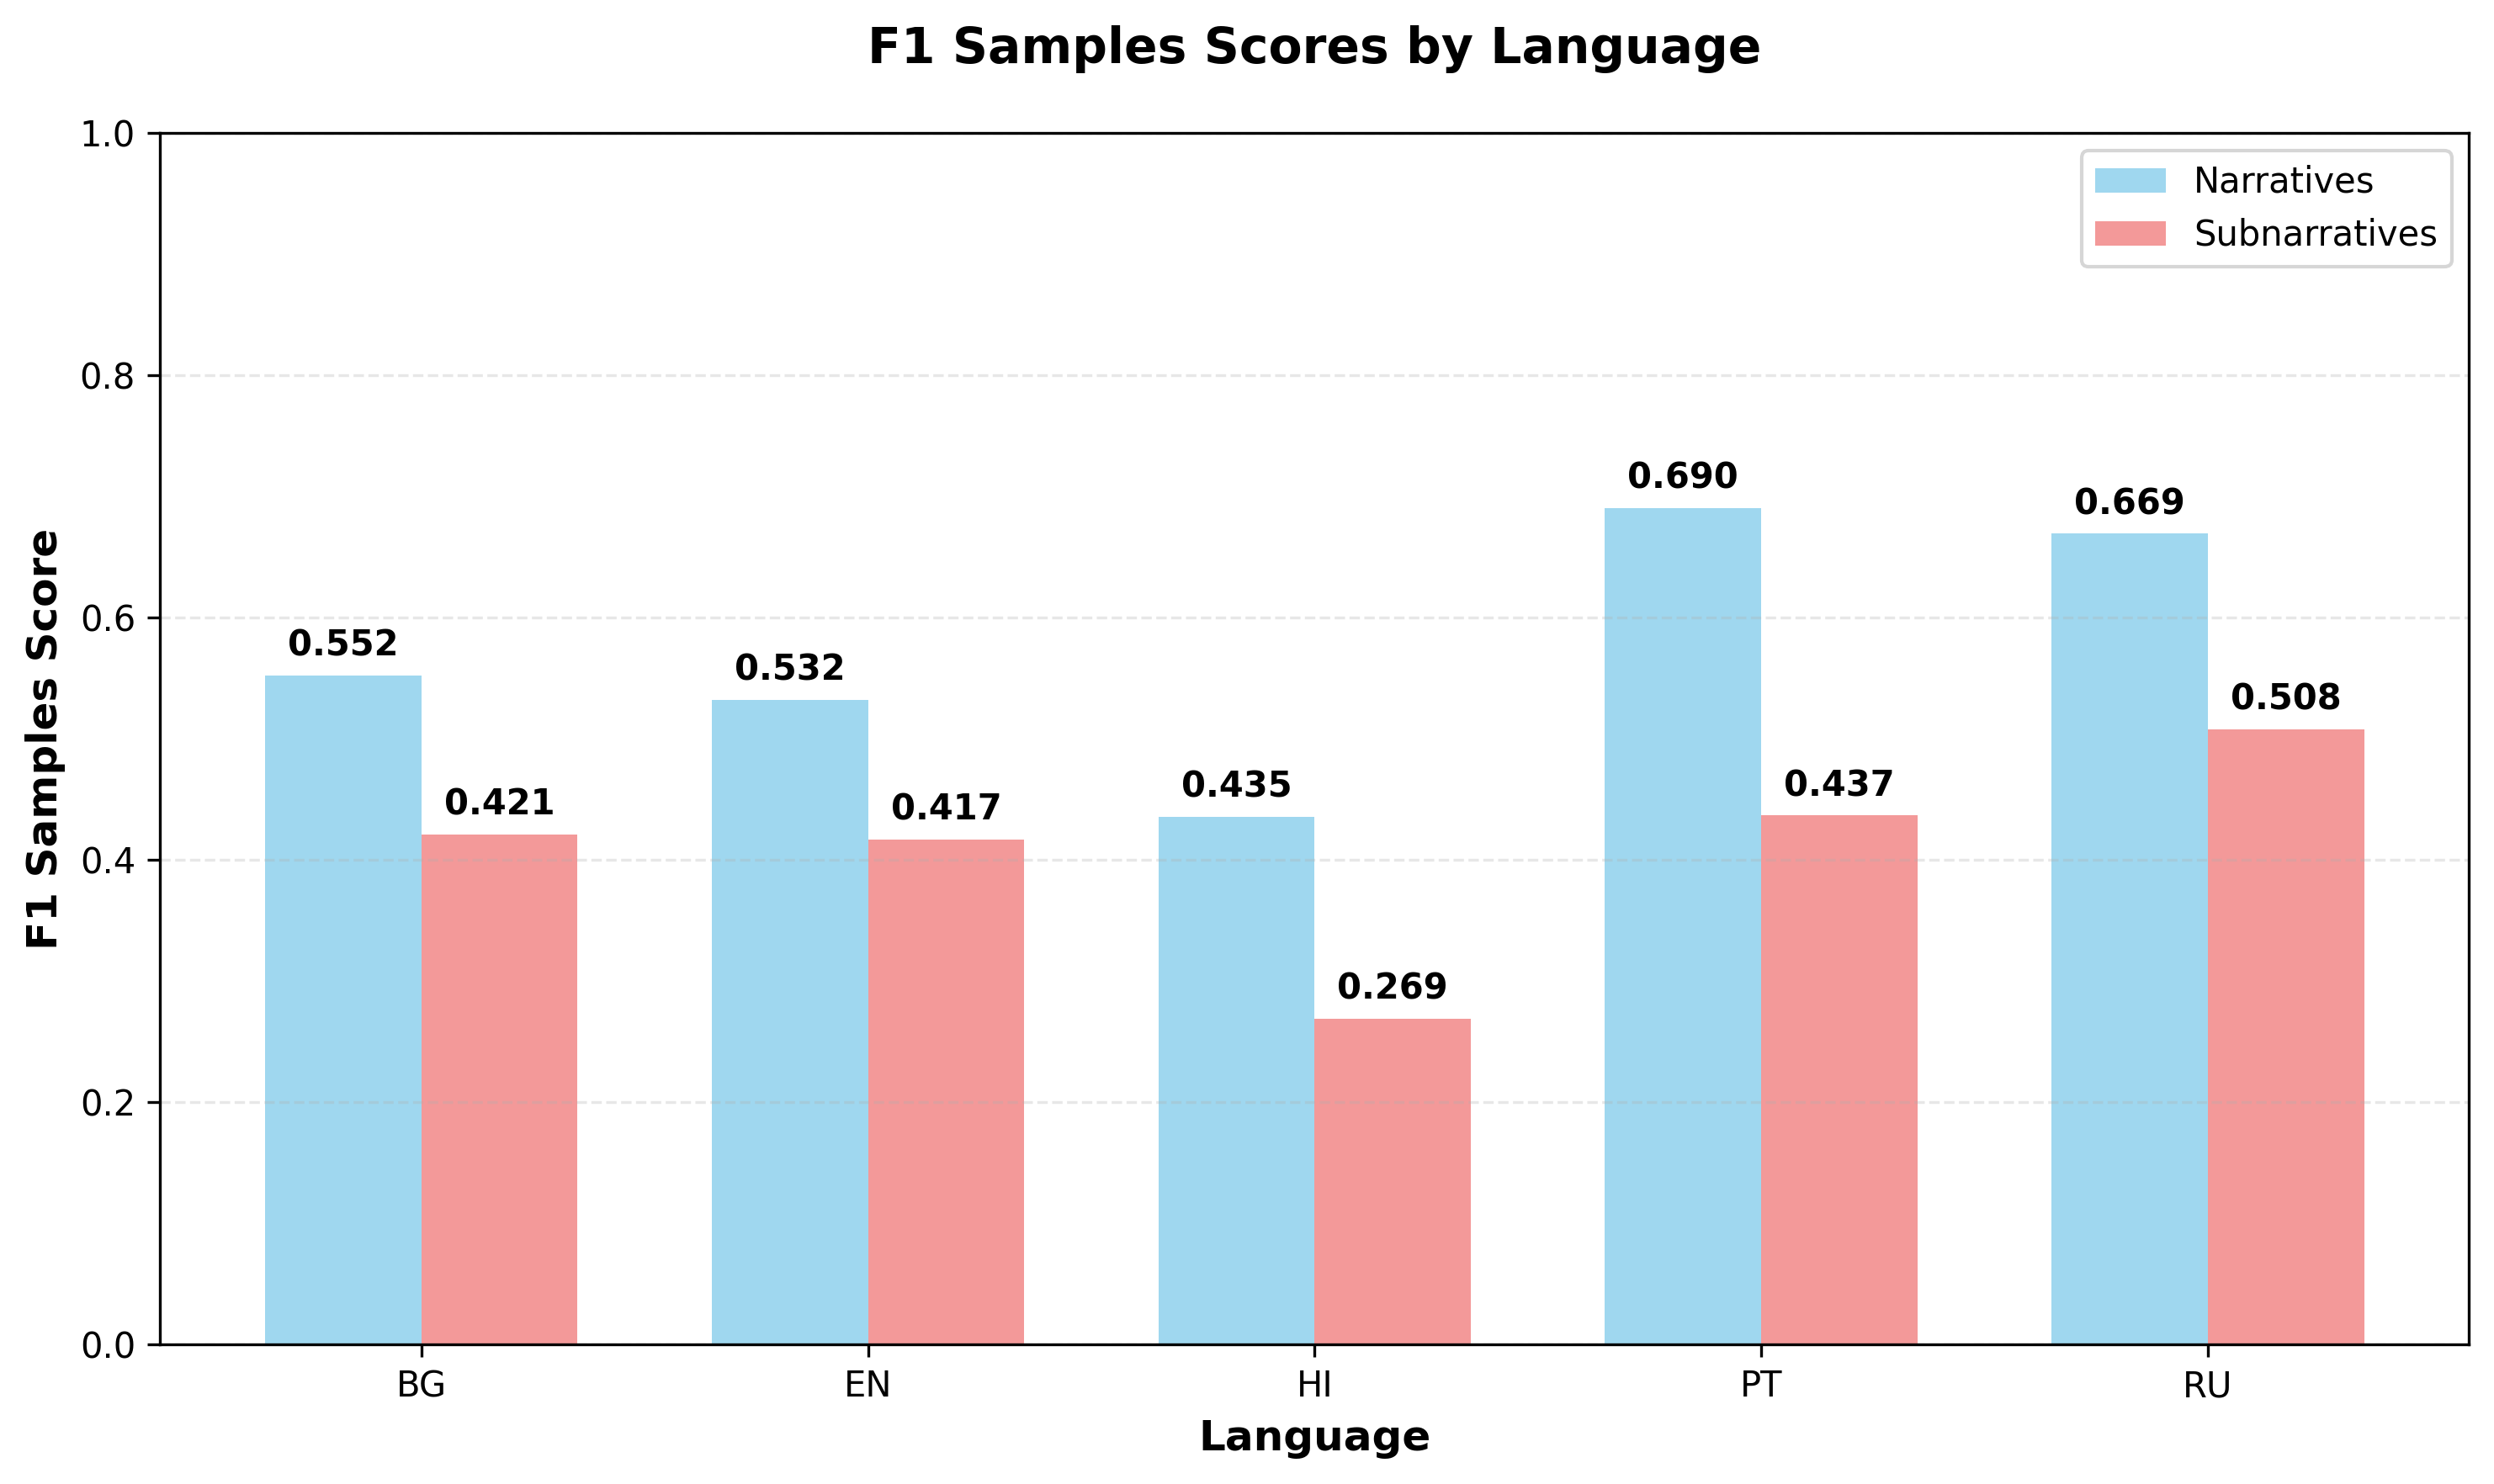
\includegraphics[width=0.85\textwidth]{gemini25_flash_subnarr_val_evaluation/plots/f1_samples_by_language.png}
    \caption{F1 Samples performance by language for the subnarrative-validation configuration.}
    \label{fig:app-subnarr-val-f1-samples}
\end{figure}

\subsection{Bulgarian (BG) Performance}

\begin{figure}[H]
    \centering
    \begin{subfigure}[b]{0.48\textwidth}
        \centering
        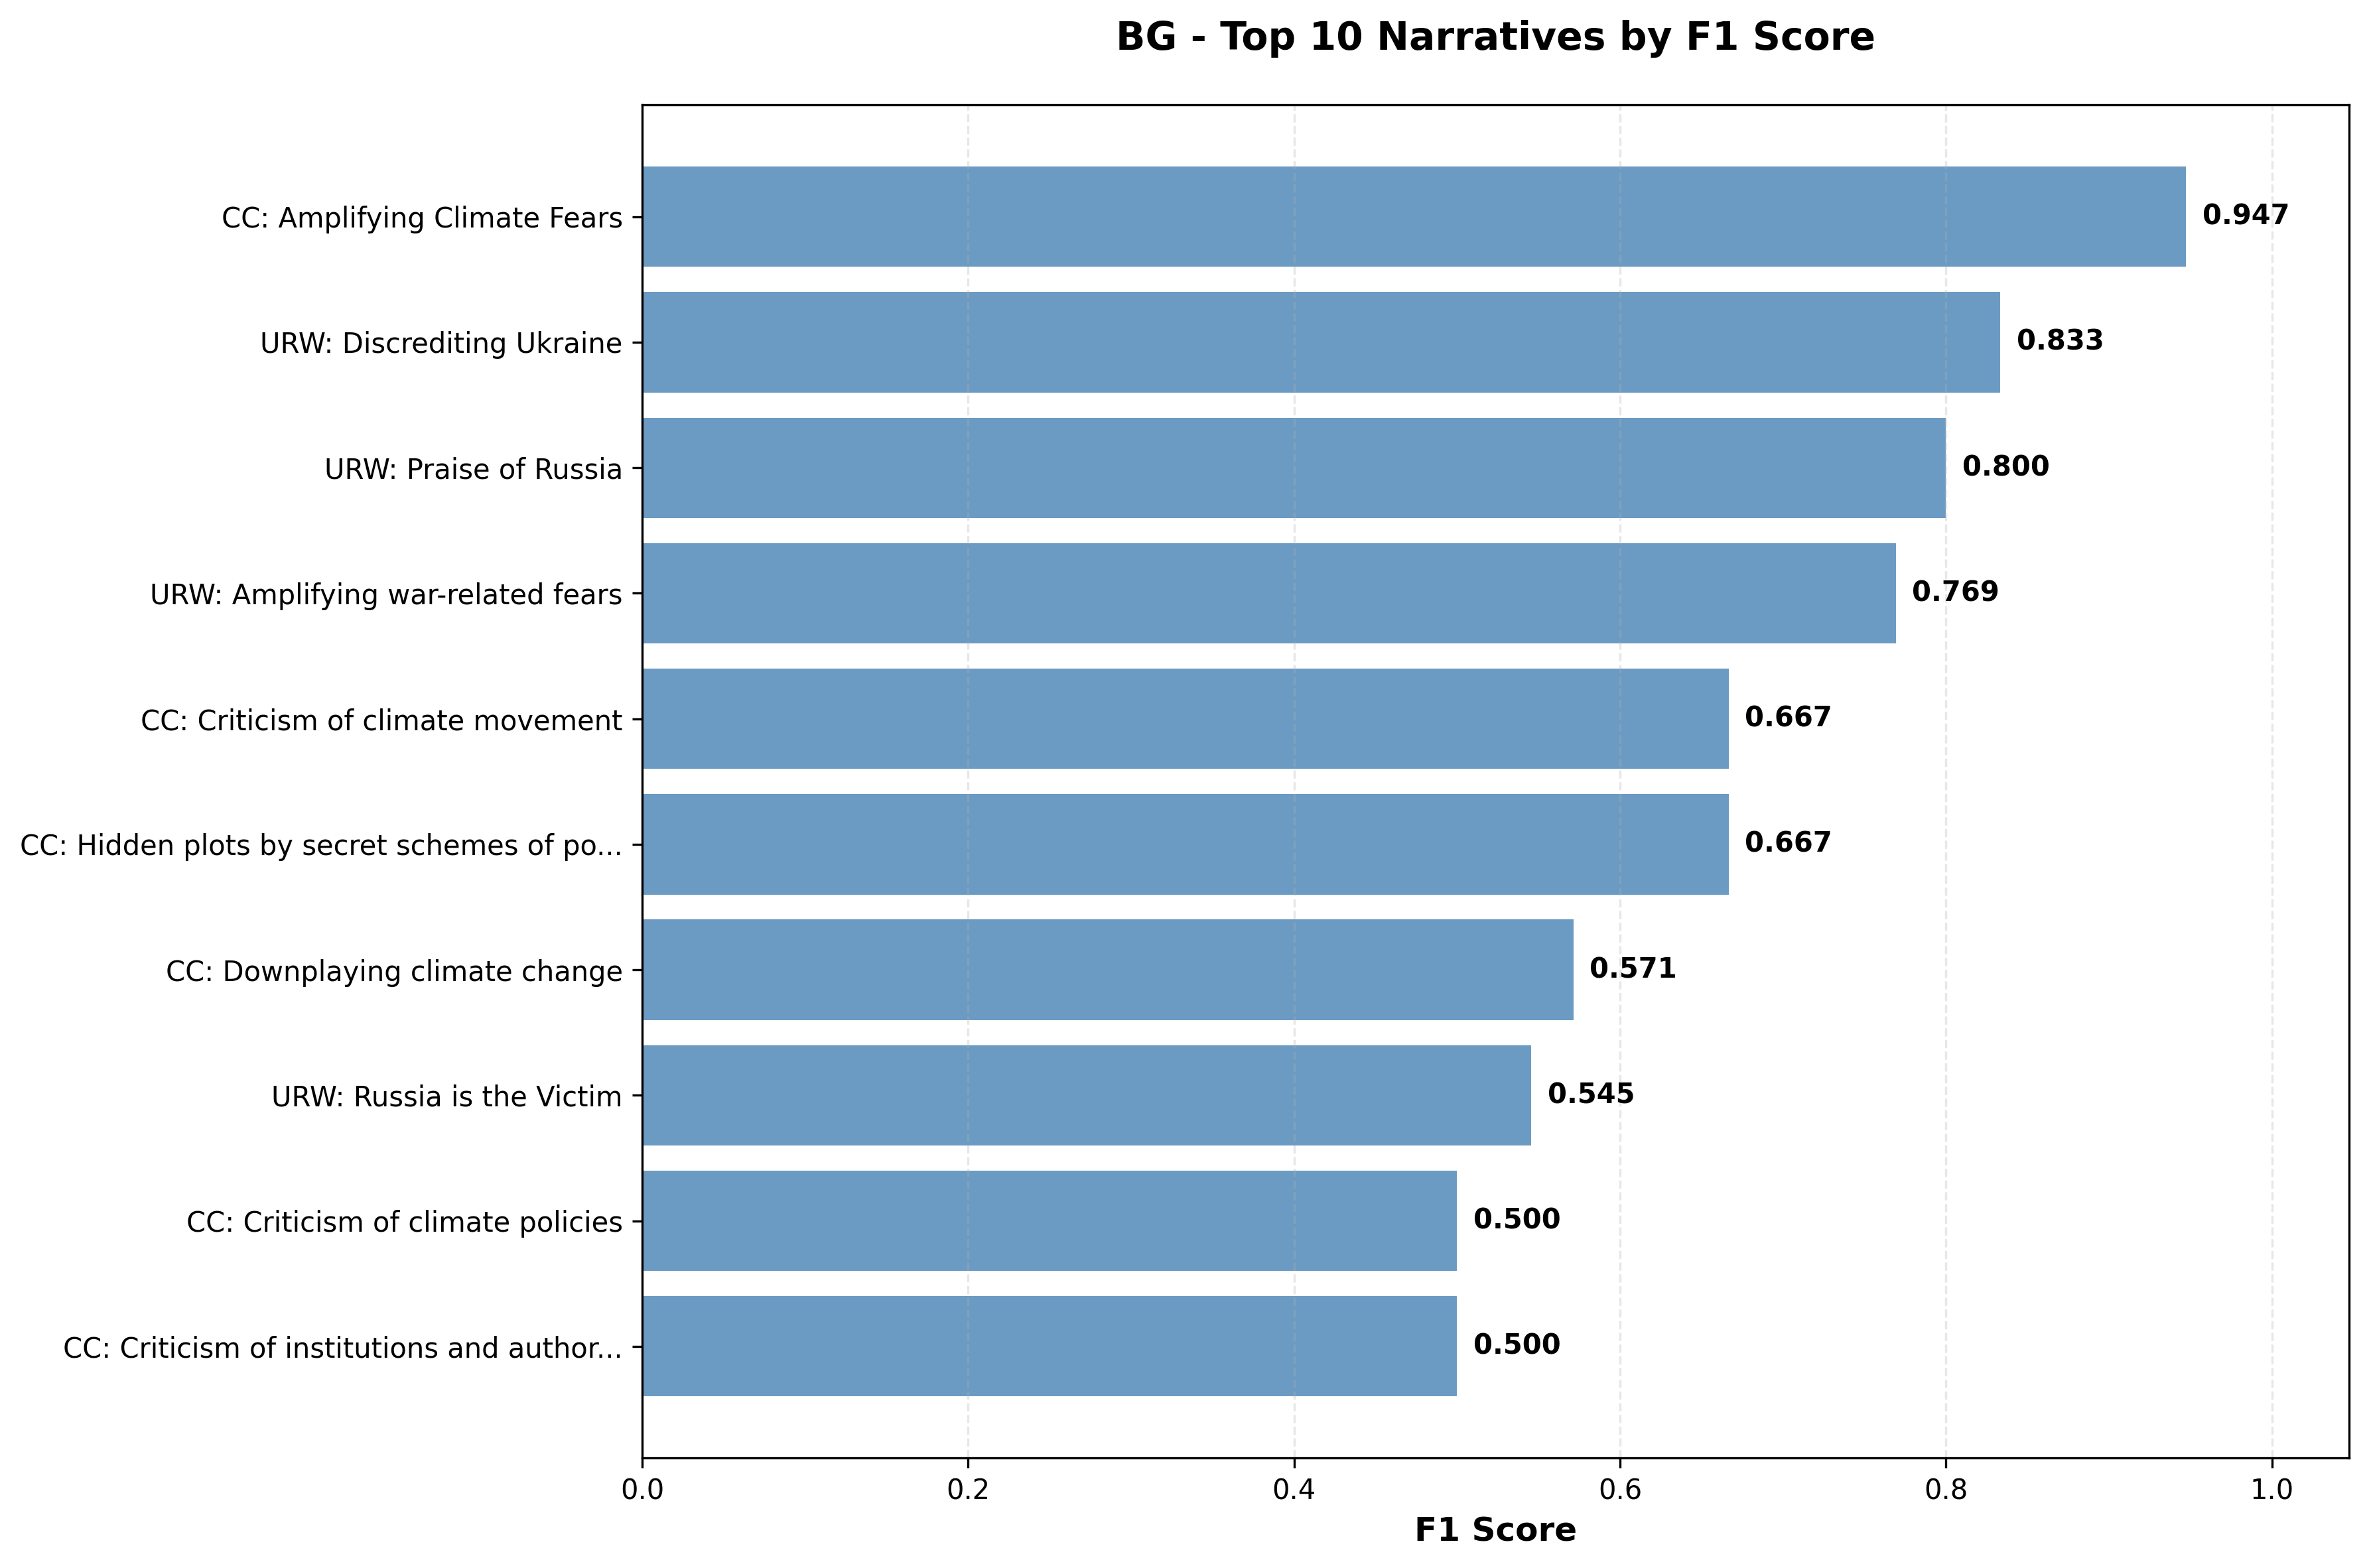
\includegraphics[width=\textwidth]{gemini25_flash_subnarr_val_evaluation/plots/BG_top_narratives_f1_scores.png}
        \caption{Top narrative F1 scores}
        \label{fig:app-subnarr-val-bg-narr}
    \end{subfigure}
    \hfill
    \begin{subfigure}[b]{0.48\textwidth}
        \centering
        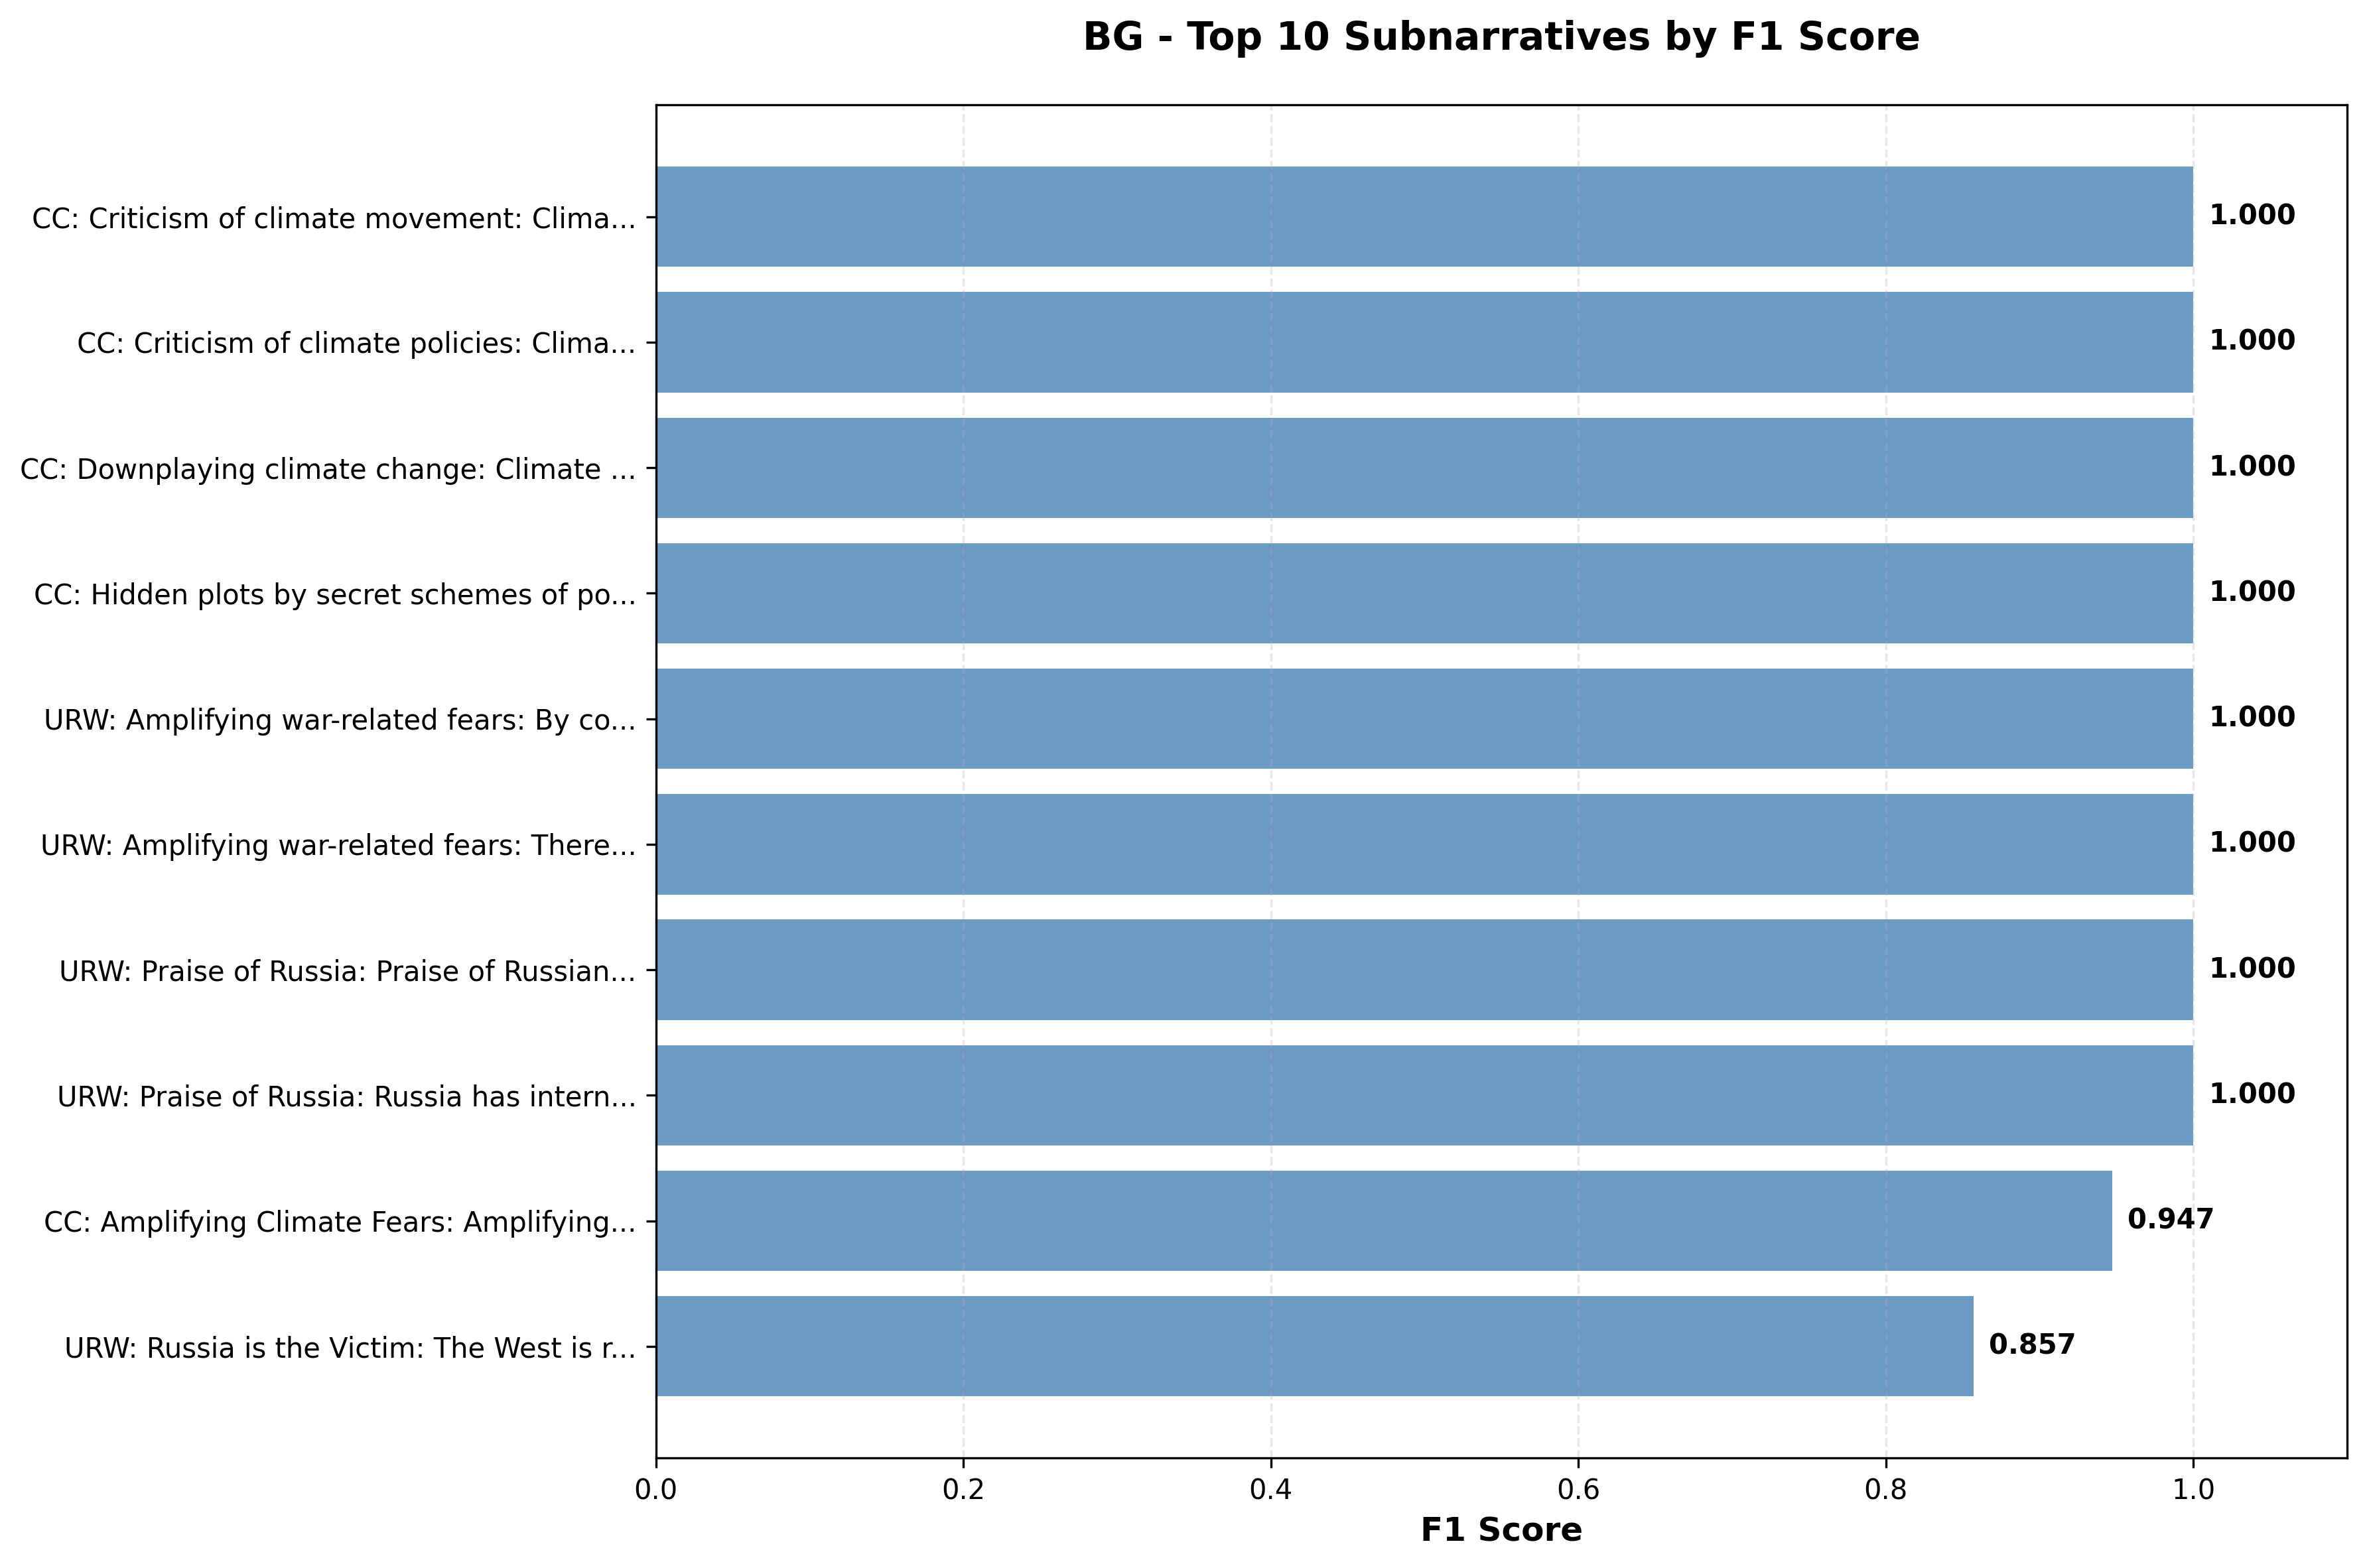
\includegraphics[width=\textwidth]{gemini25_flash_subnarr_val_evaluation/plots/BG_top_subnarratives_f1_scores.png}
        \caption{Top subnarrative F1 scores}
        \label{fig:app-subnarr-val-bg-subnarr}
    \end{subfigure}
    \caption{Bulgarian performance breakdown for subnarrative-validation configuration.}
    \label{fig:app-subnarr-val-bg}
\end{figure}

\subsection{English (EN) Performance}

\begin{figure}[H]
    \centering
    \begin{subfigure}[b]{0.48\textwidth}
        \centering
        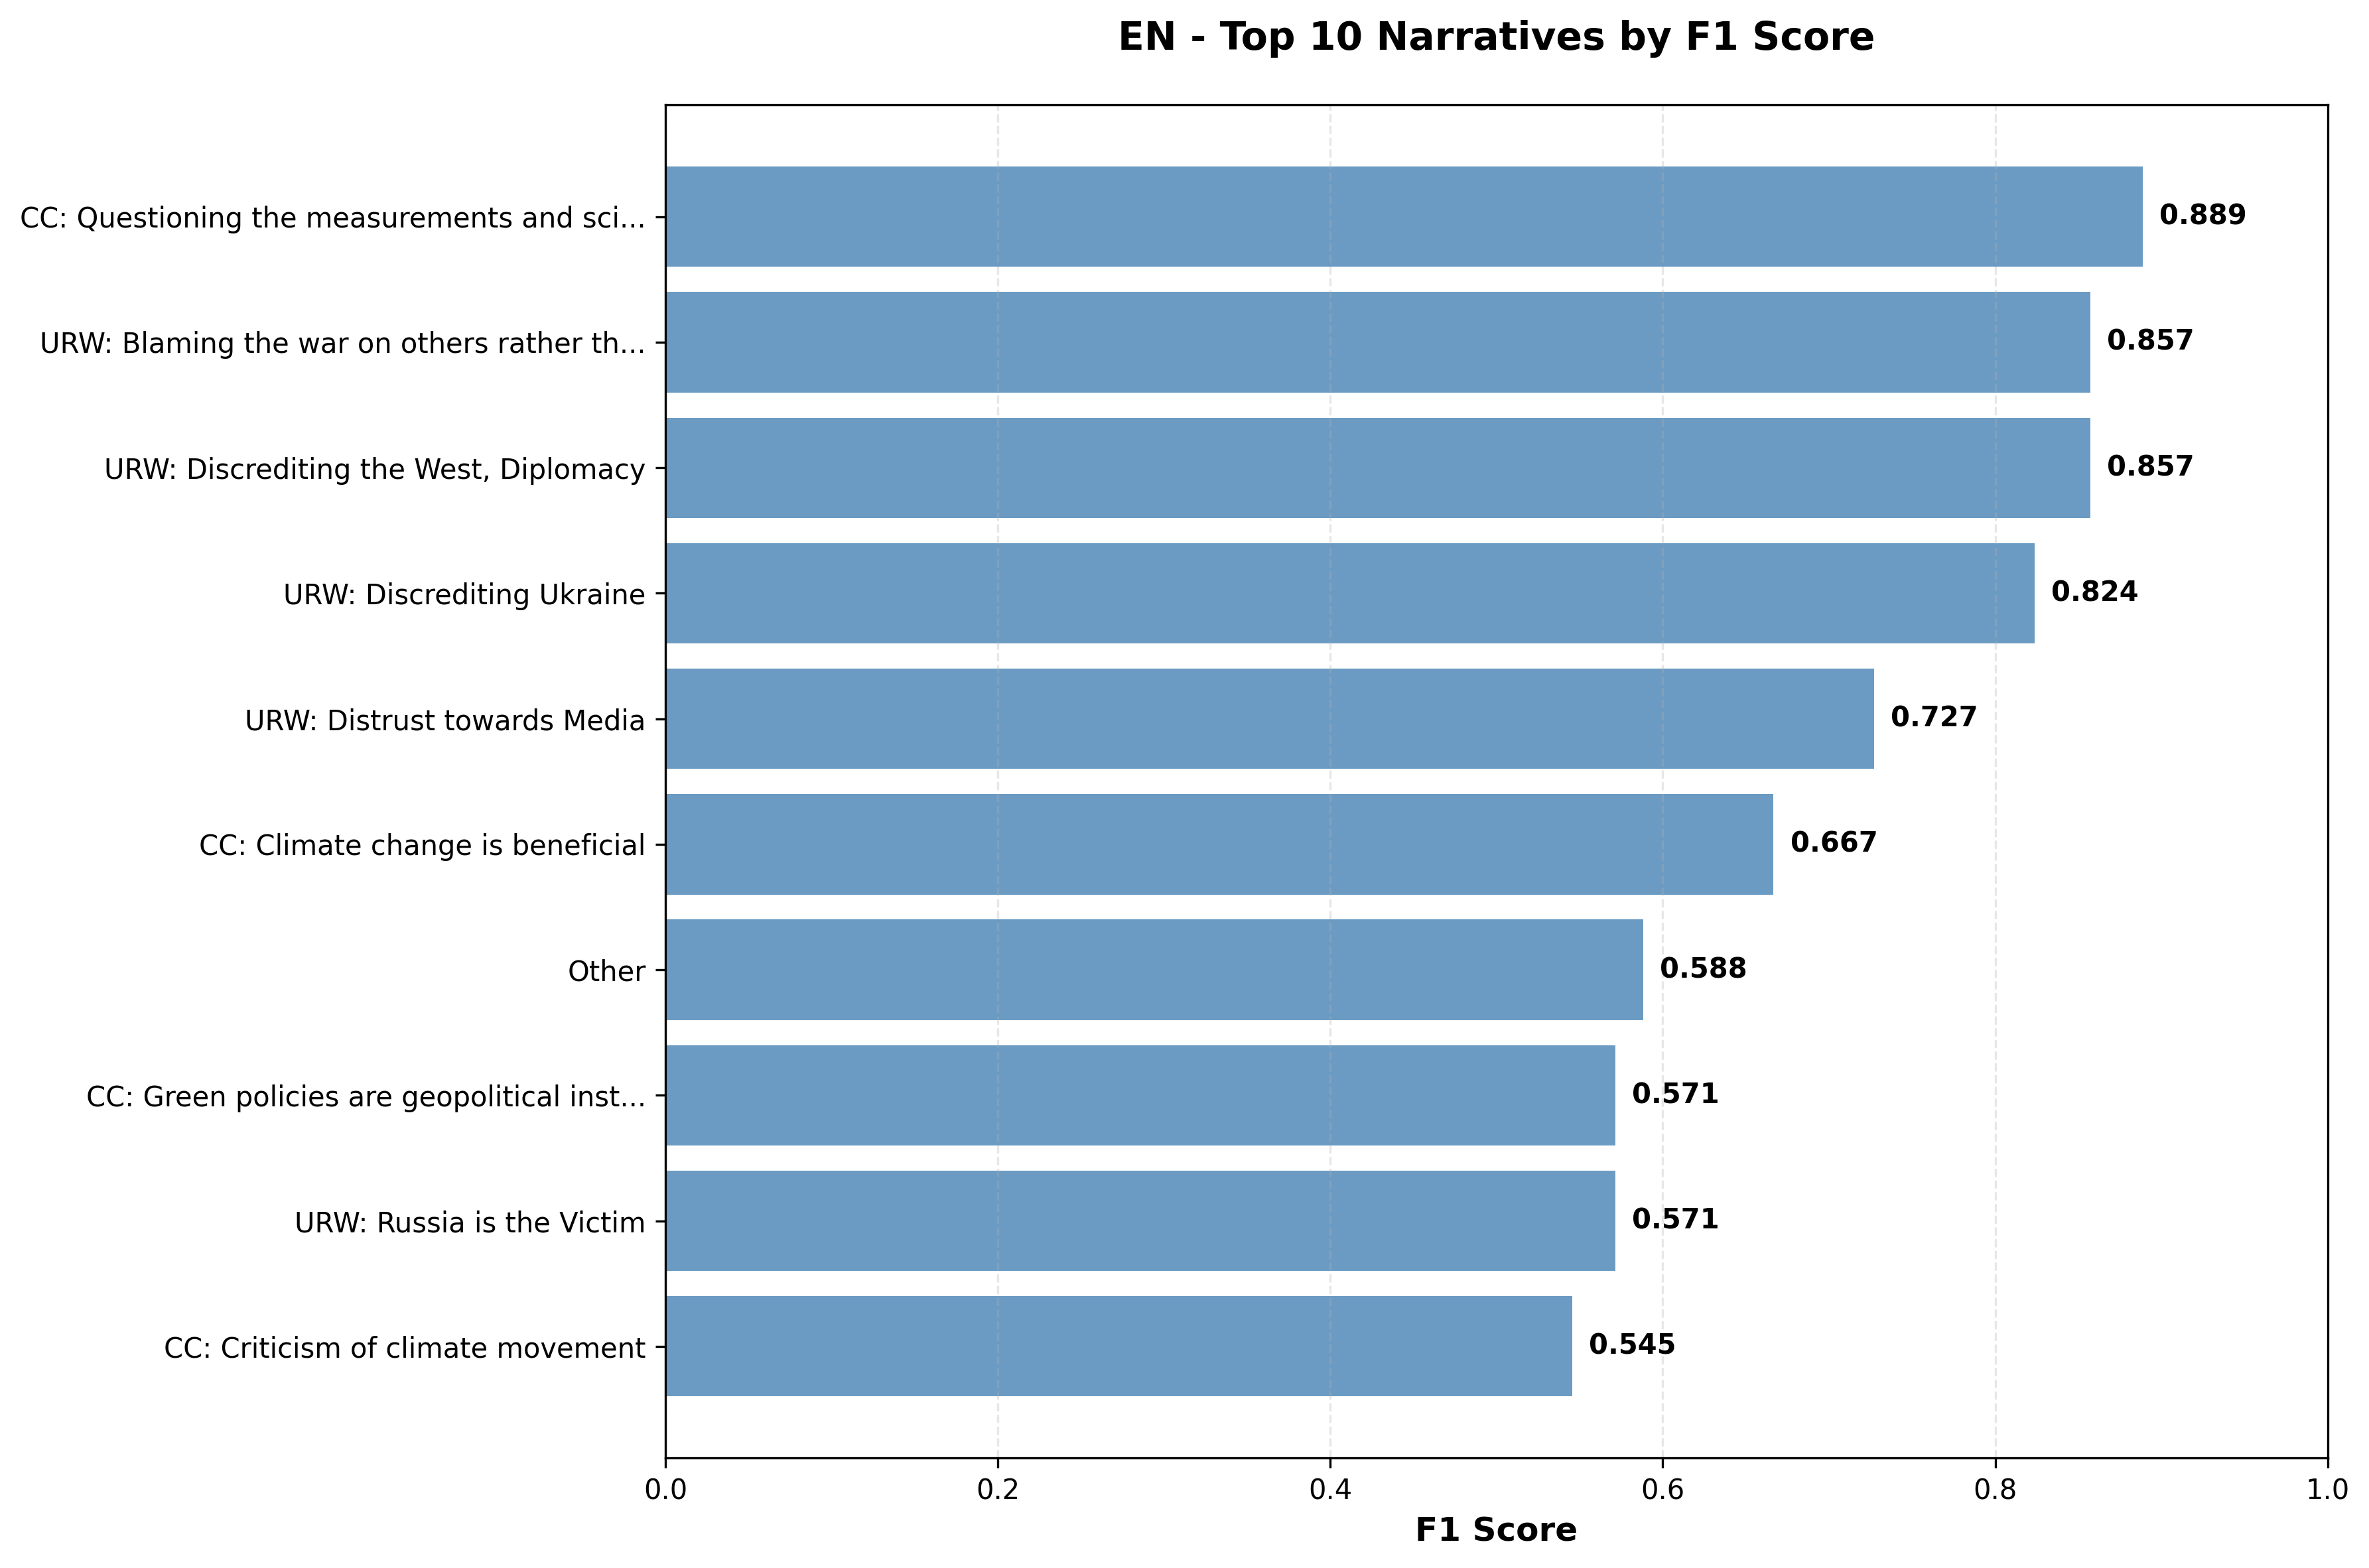
\includegraphics[width=\textwidth]{gemini25_flash_subnarr_val_evaluation/plots/EN_top_narratives_f1_scores.png}
        \caption{Top narrative F1 scores}
        \label{fig:app-subnarr-val-en-narr}
    \end{subfigure}
    \hfill
    \begin{subfigure}[b]{0.48\textwidth}
        \centering
        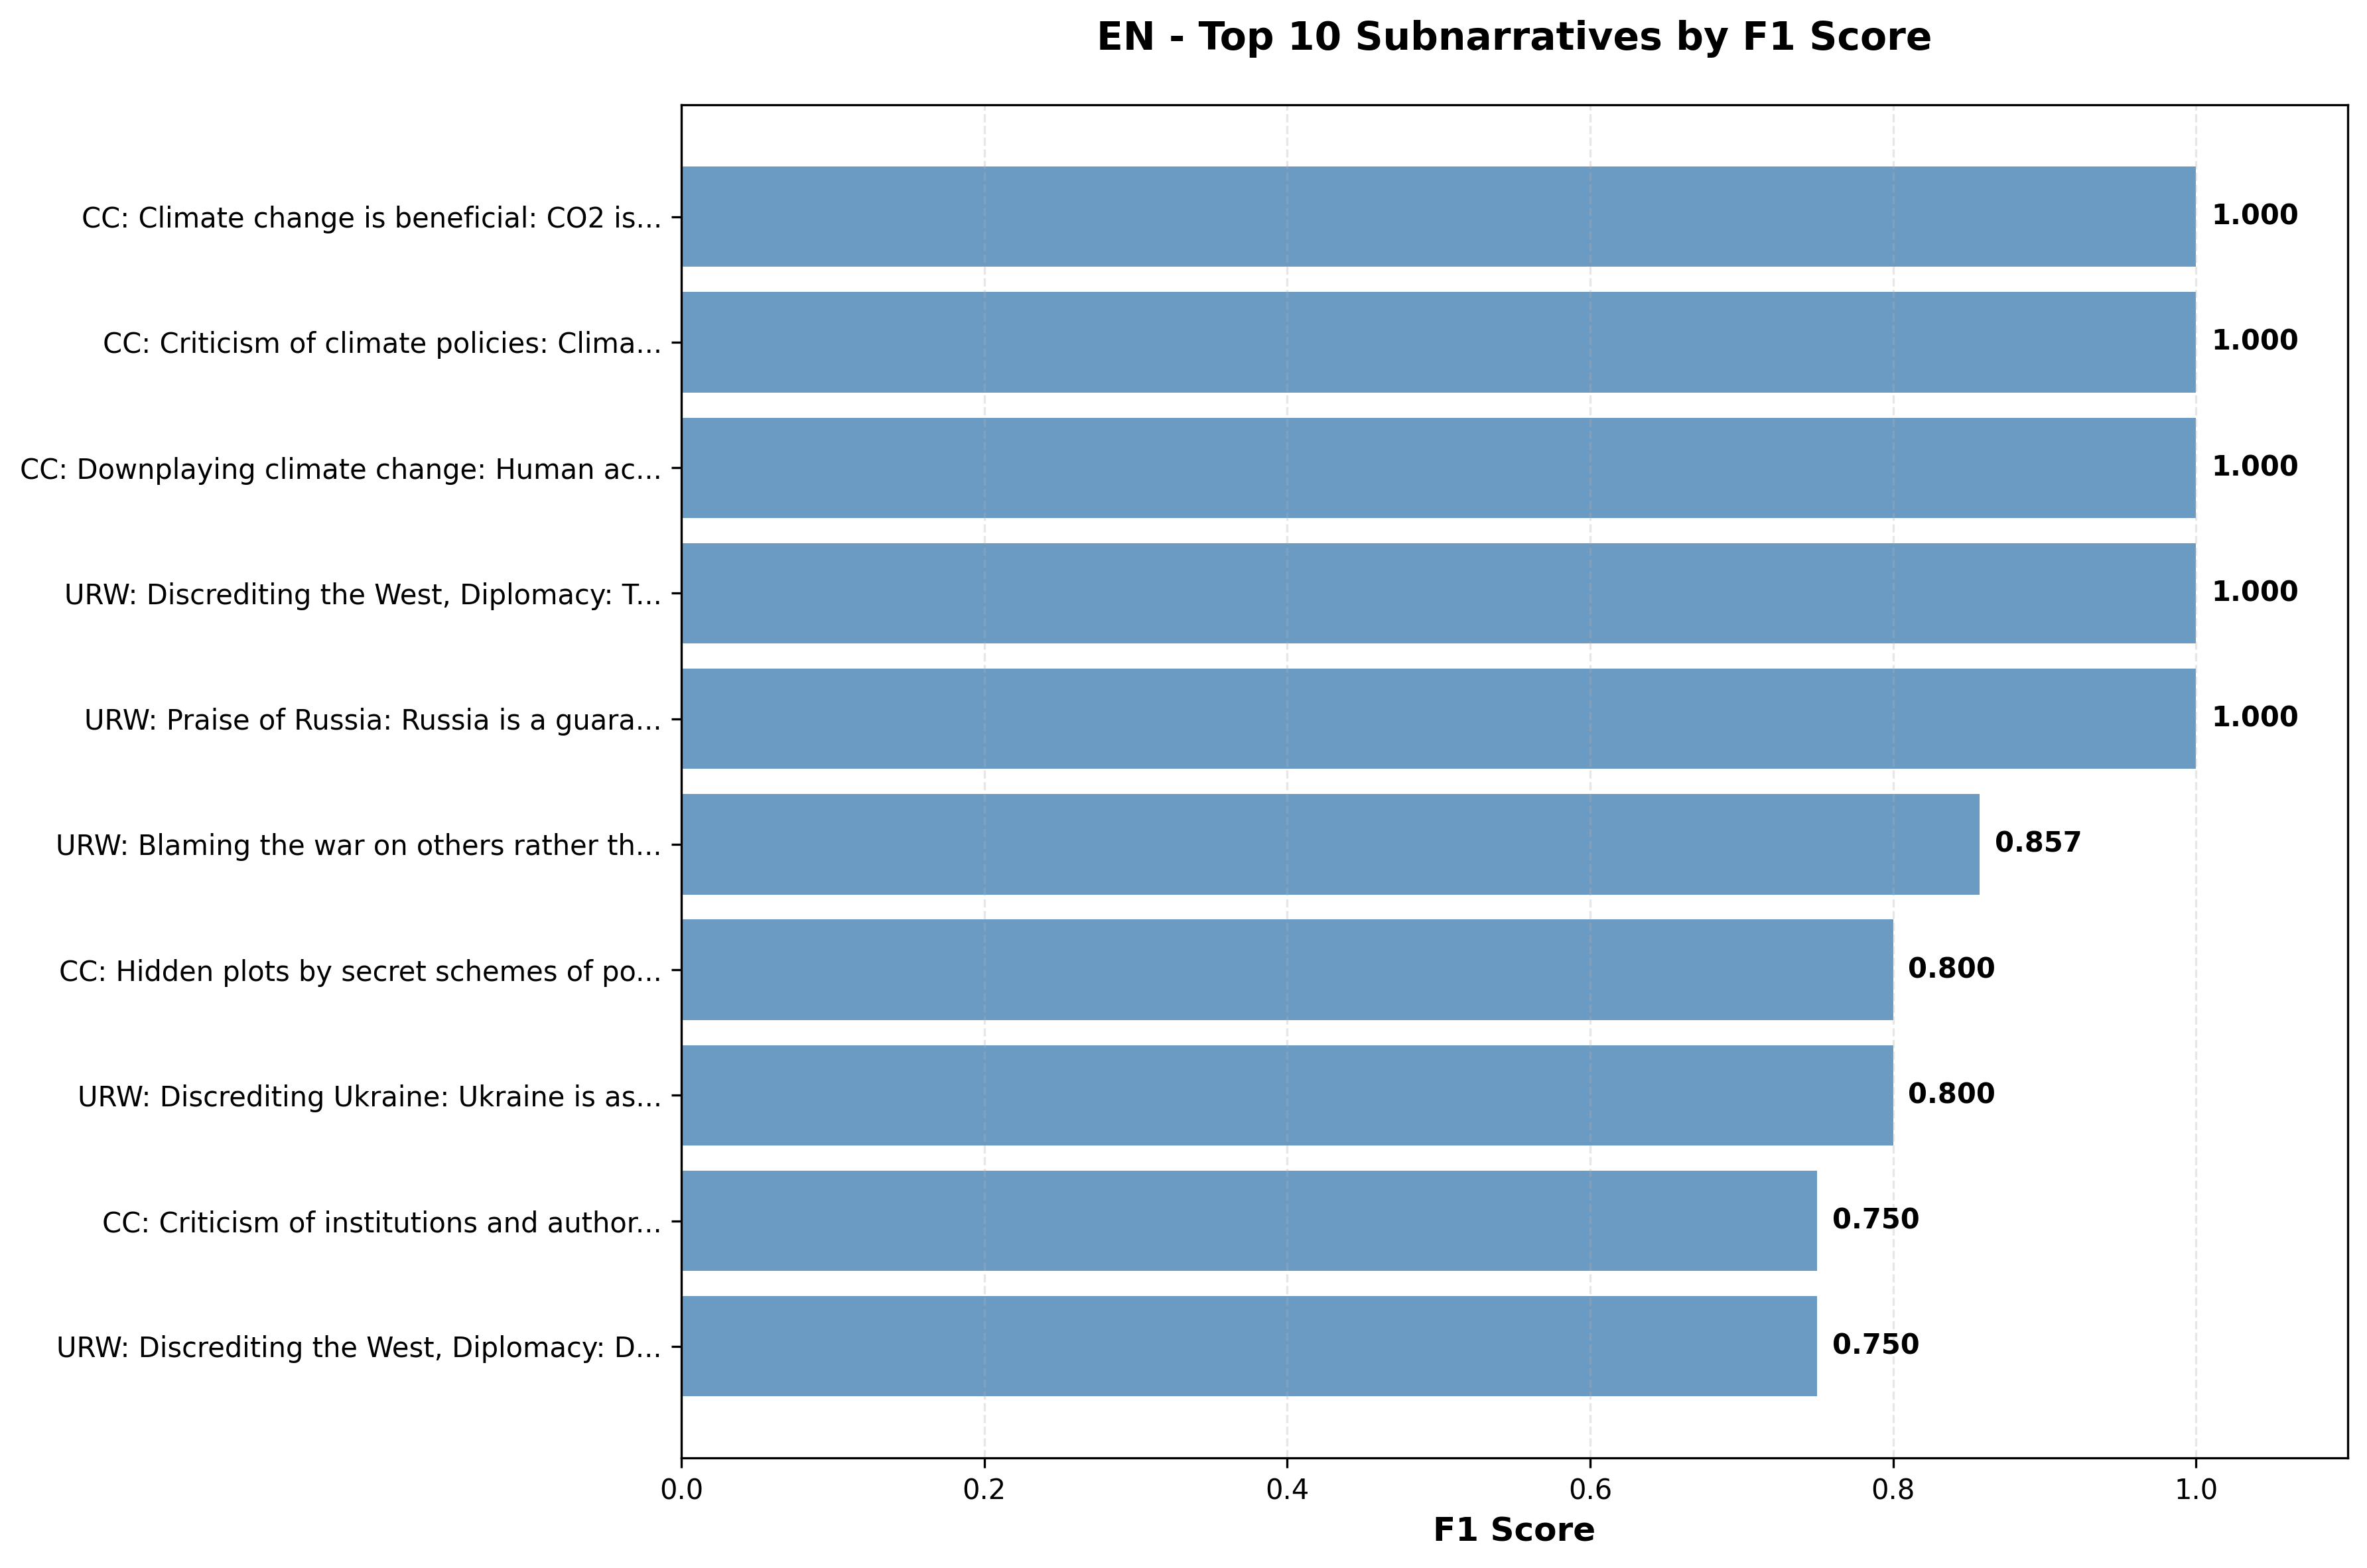
\includegraphics[width=\textwidth]{gemini25_flash_subnarr_val_evaluation/plots/EN_top_subnarratives_f1_scores.png}
        \caption{Top subnarrative F1 scores}
        \label{fig:app-subnarr-val-en-subnarr}
    \end{subfigure}
    \caption{English performance breakdown for subnarrative-validation configuration.}
    \label{fig:app-subnarr-val-en}
\end{figure}

\subsection{Hindi (HI) Performance}

\begin{figure}[H]
    \centering
    \begin{subfigure}[b]{0.48\textwidth}
        \centering
        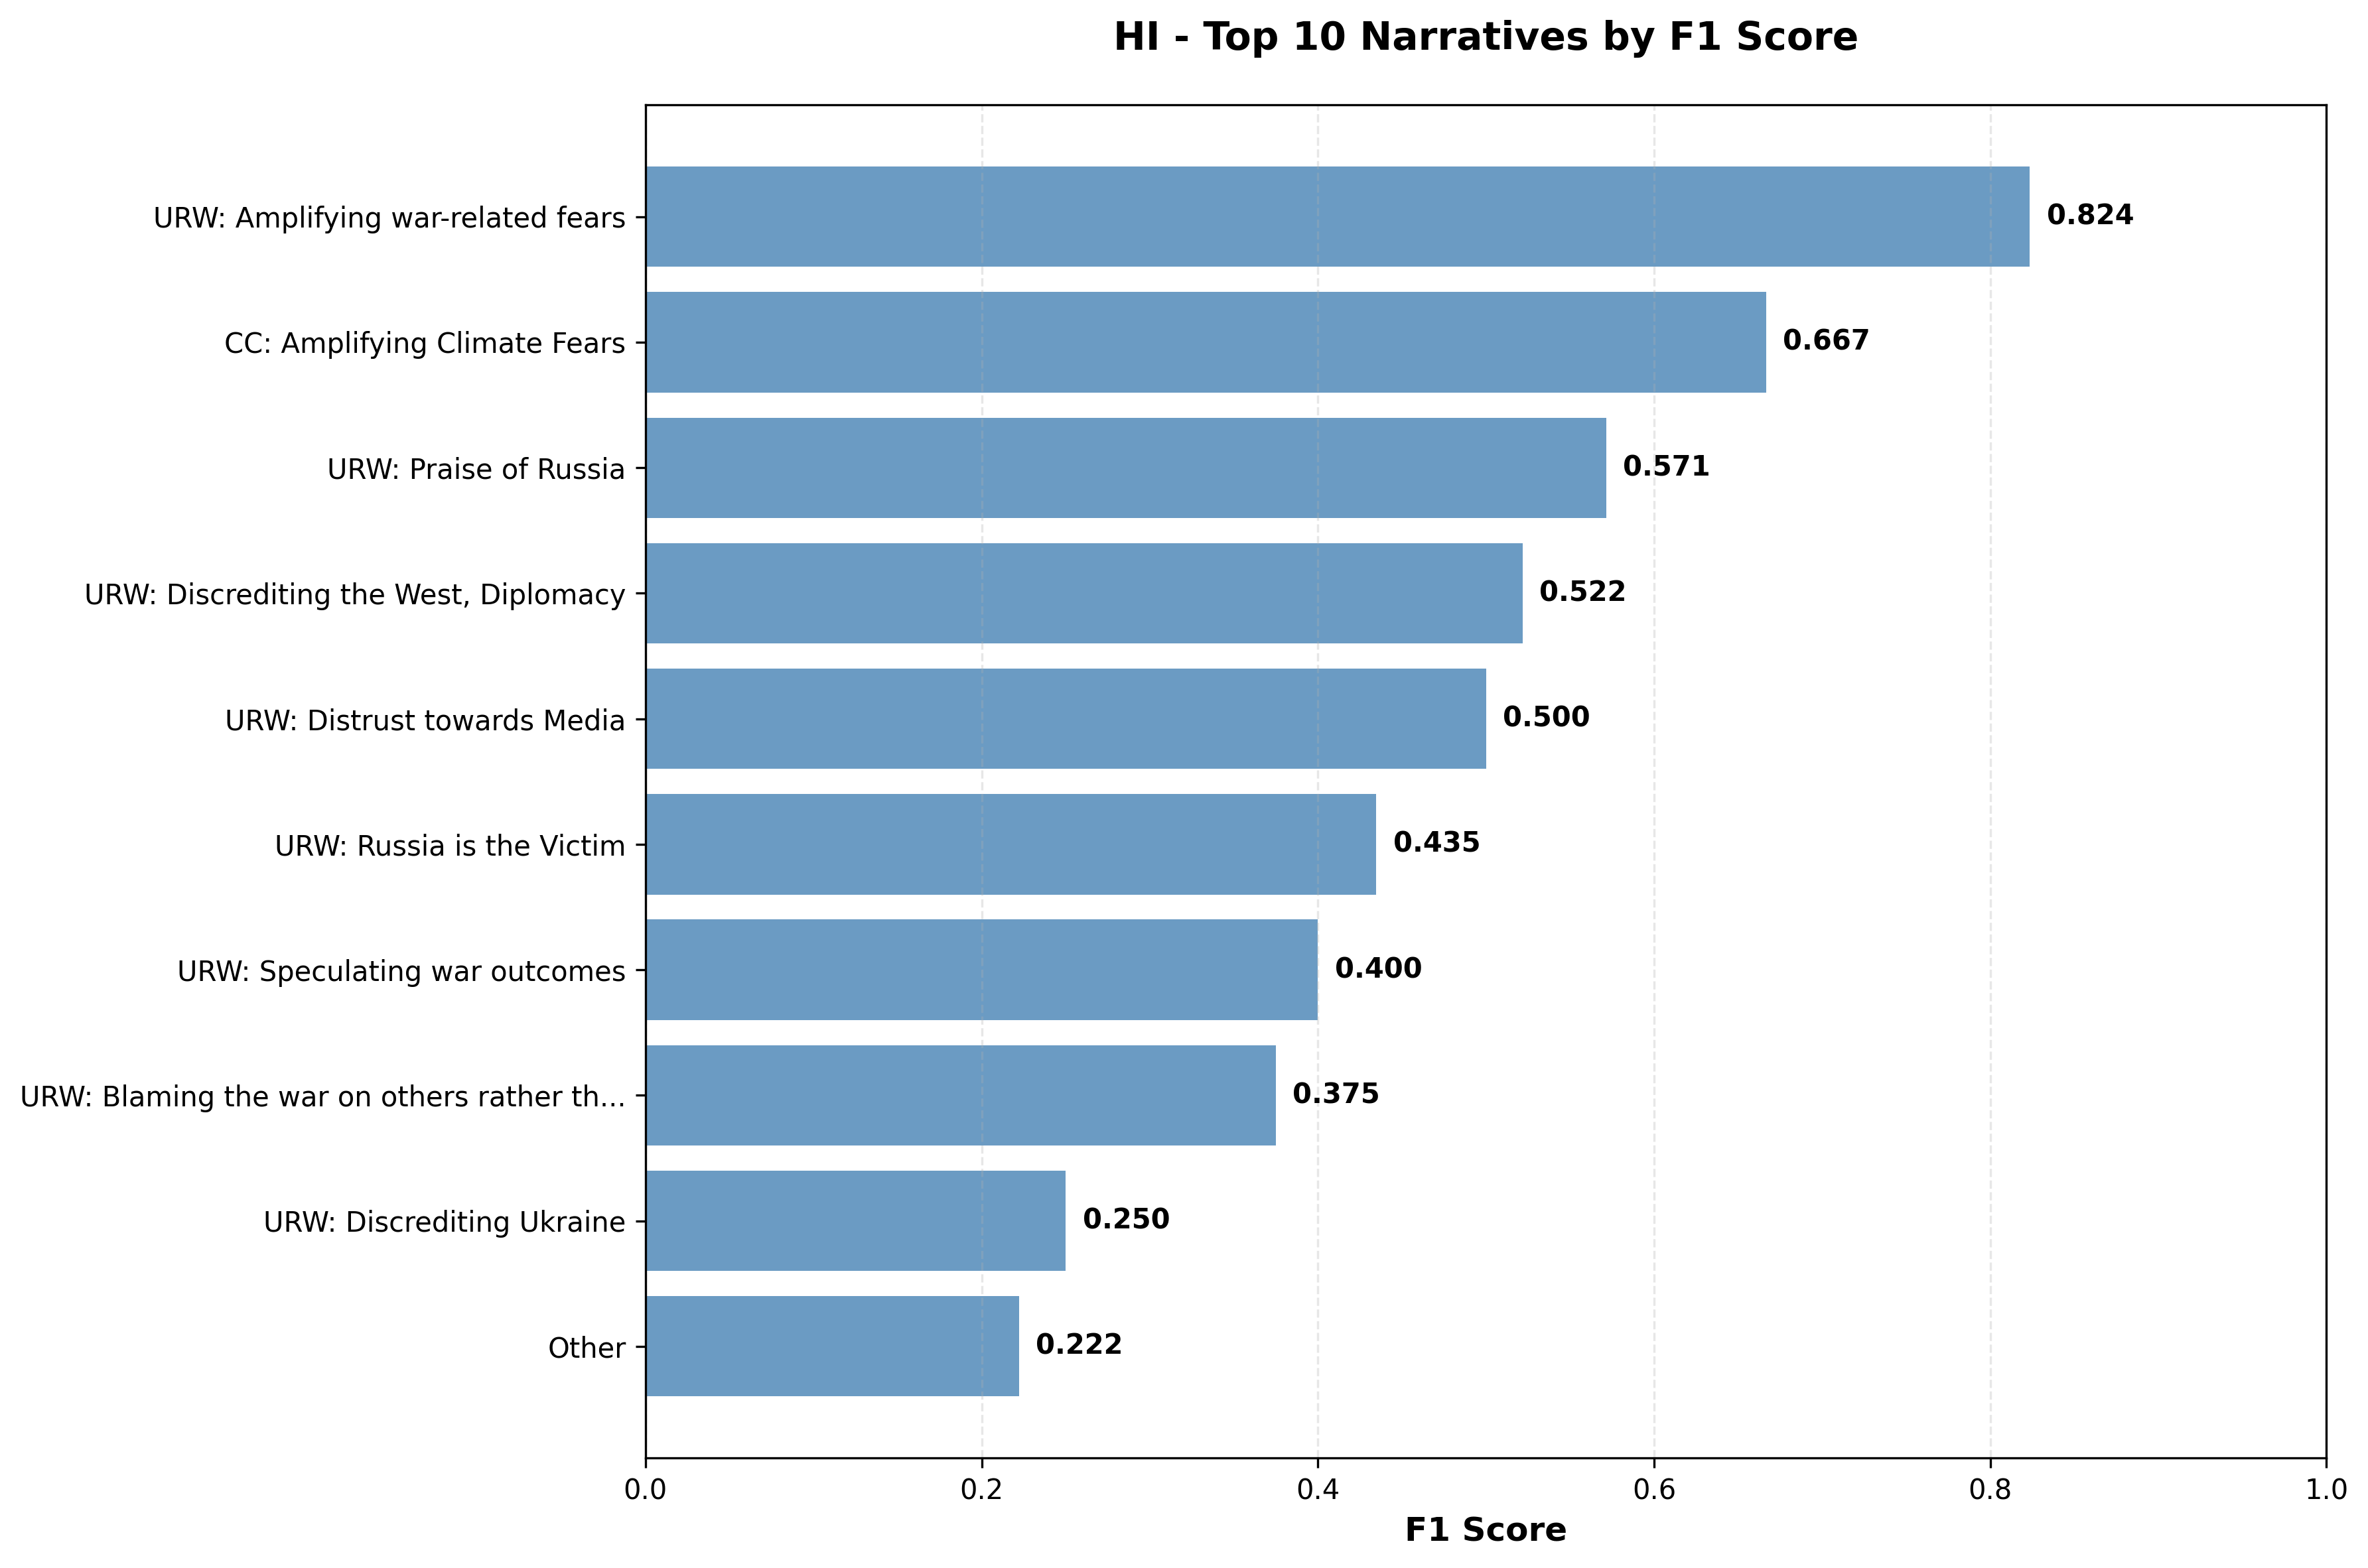
\includegraphics[width=\textwidth]{gemini25_flash_subnarr_val_evaluation/plots/HI_top_narratives_f1_scores.png}
        \caption{Top narrative F1 scores}
        \label{fig:app-subnarr-val-hi-narr}
    \end{subfigure}
    \hfill
    \begin{subfigure}[b]{0.48\textwidth}
        \centering
        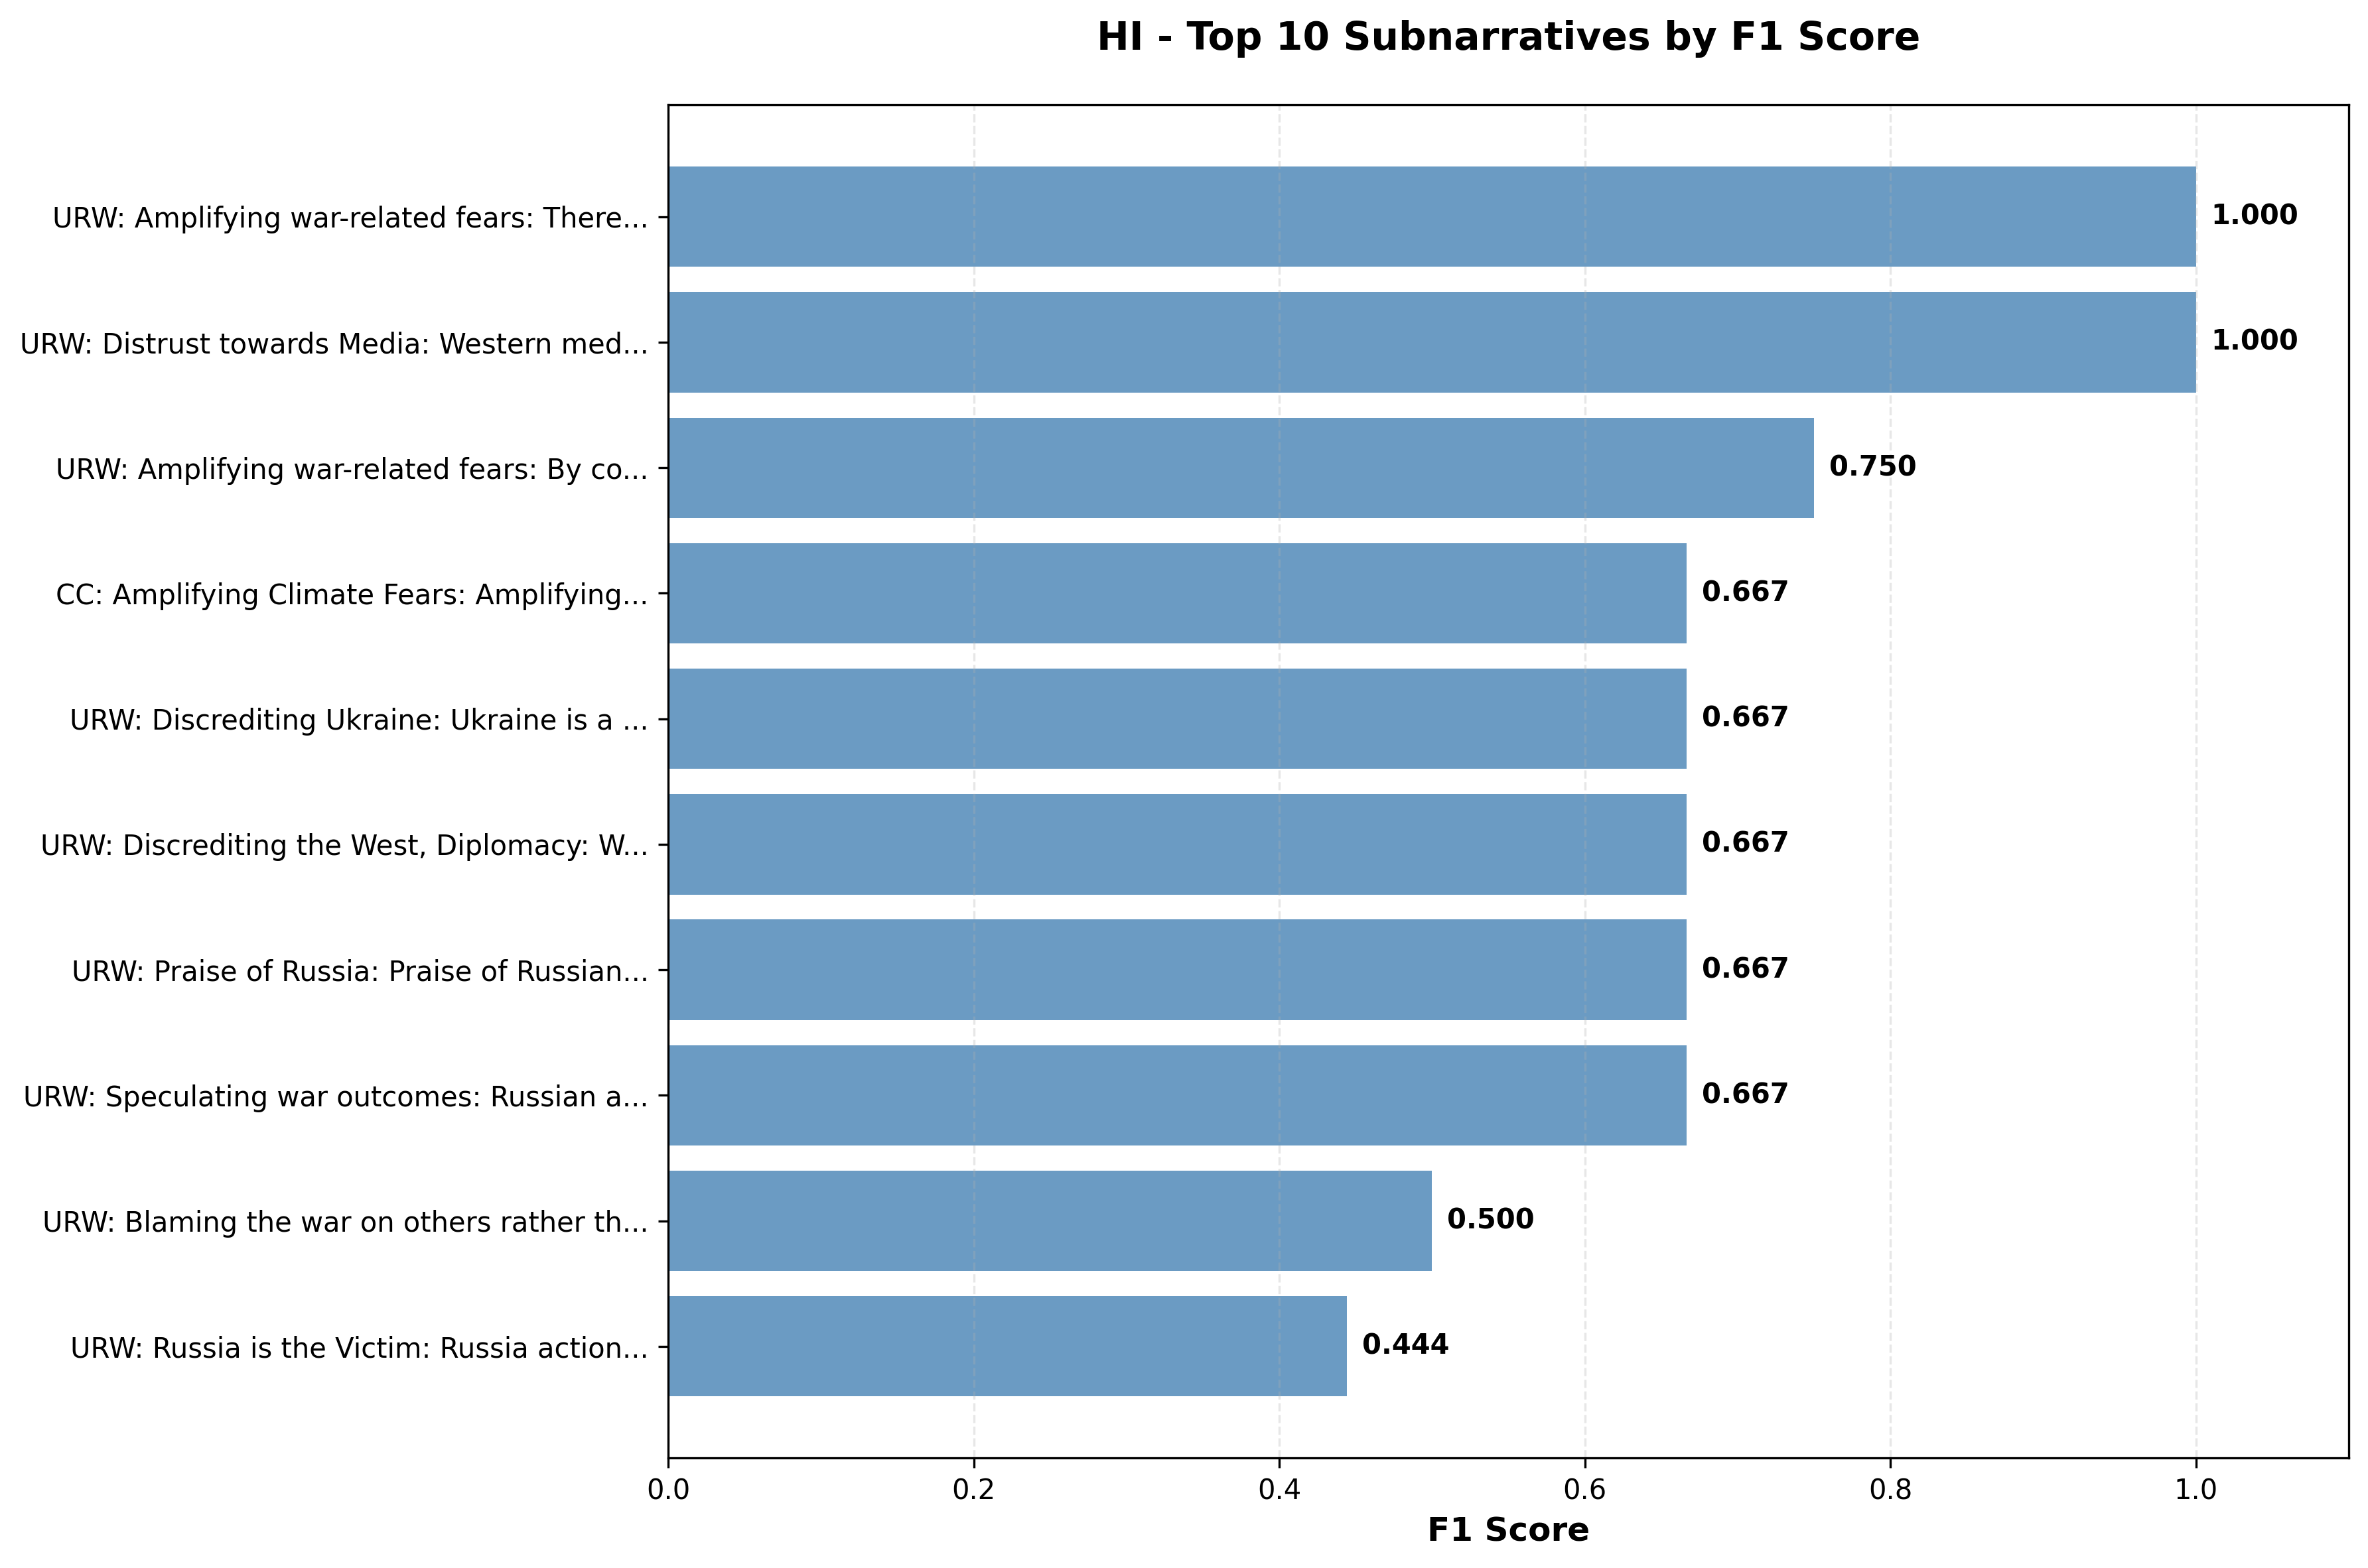
\includegraphics[width=\textwidth]{gemini25_flash_subnarr_val_evaluation/plots/HI_top_subnarratives_f1_scores.png}
        \caption{Top subnarrative F1 scores}
        \label{fig:app-subnarr-val-hi-subnarr}
    \end{subfigure}
    \caption{Hindi performance breakdown for subnarrative-validation configuration.}
    \label{fig:app-subnarr-val-hi}
\end{figure}

\subsection{Portuguese (PT) Performance}

\begin{figure}[H]
    \centering
    \begin{subfigure}[b]{0.48\textwidth}
        \centering
        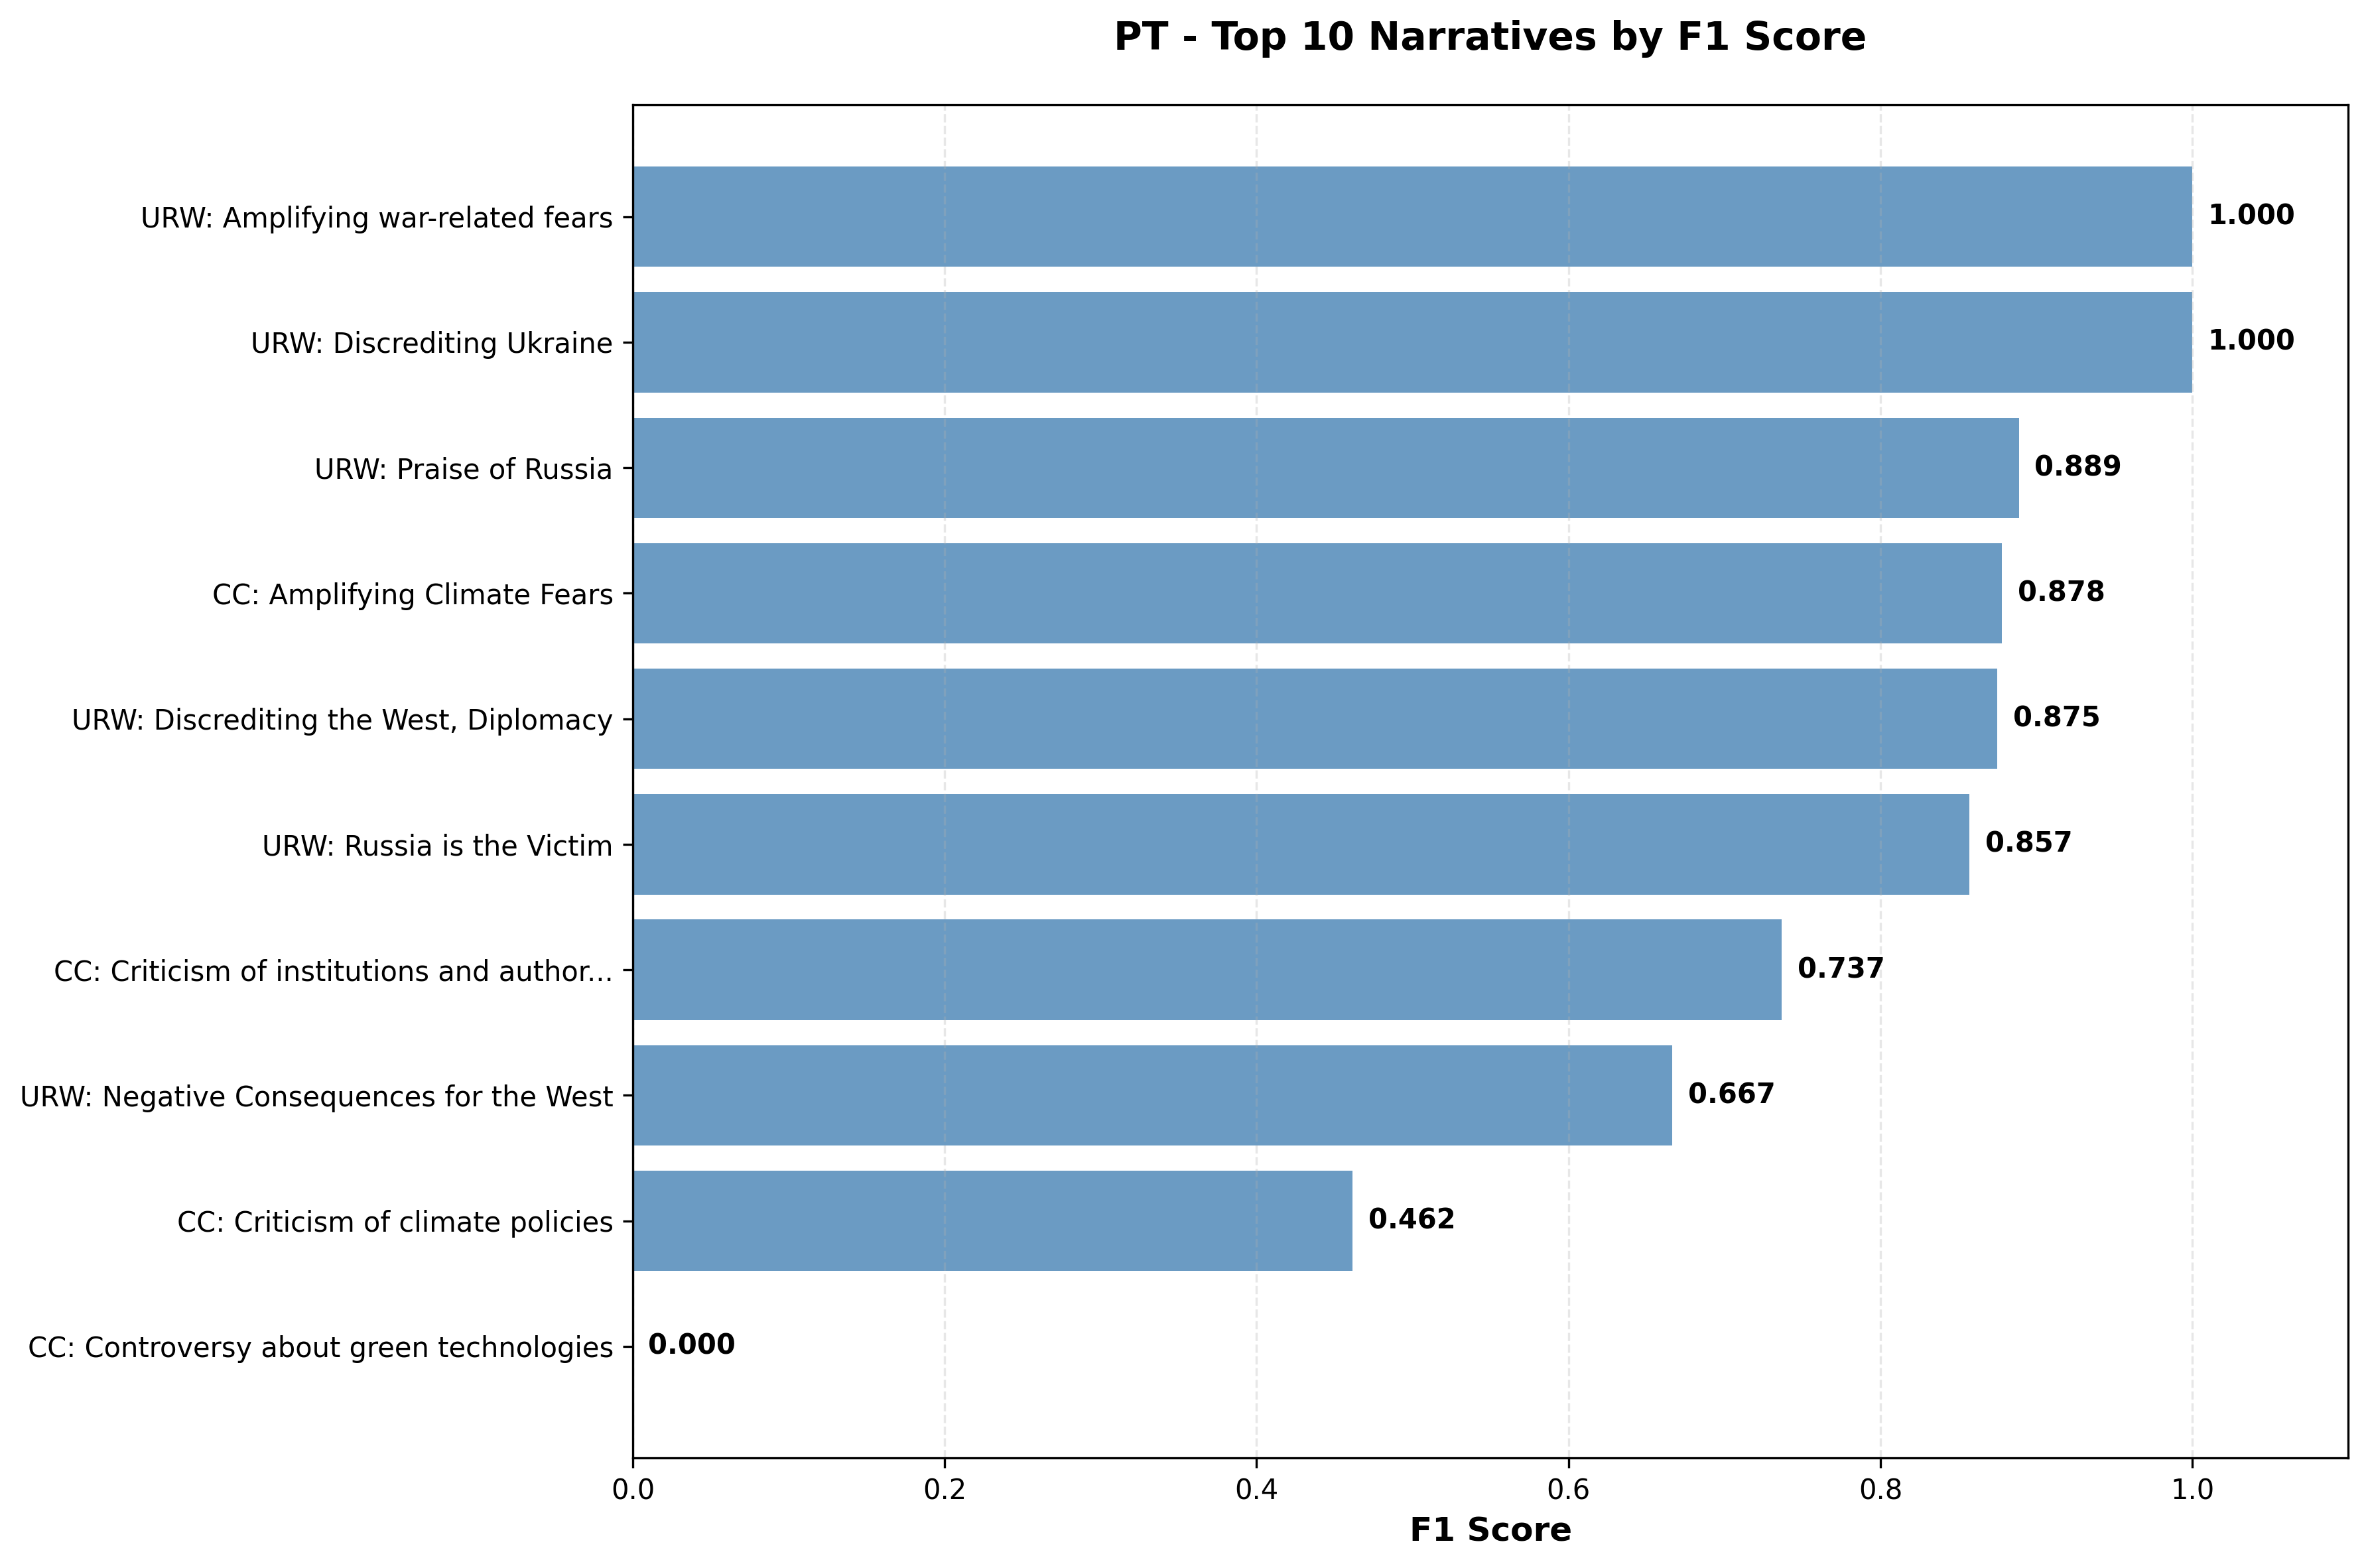
\includegraphics[width=\textwidth]{gemini25_flash_subnarr_val_evaluation/plots/PT_top_narratives_f1_scores.png}
        \caption{Top narrative F1 scores}
        \label{fig:app-subnarr-val-pt-narr}
    \end{subfigure}
    \hfill
    \begin{subfigure}[b]{0.48\textwidth}
        \centering
        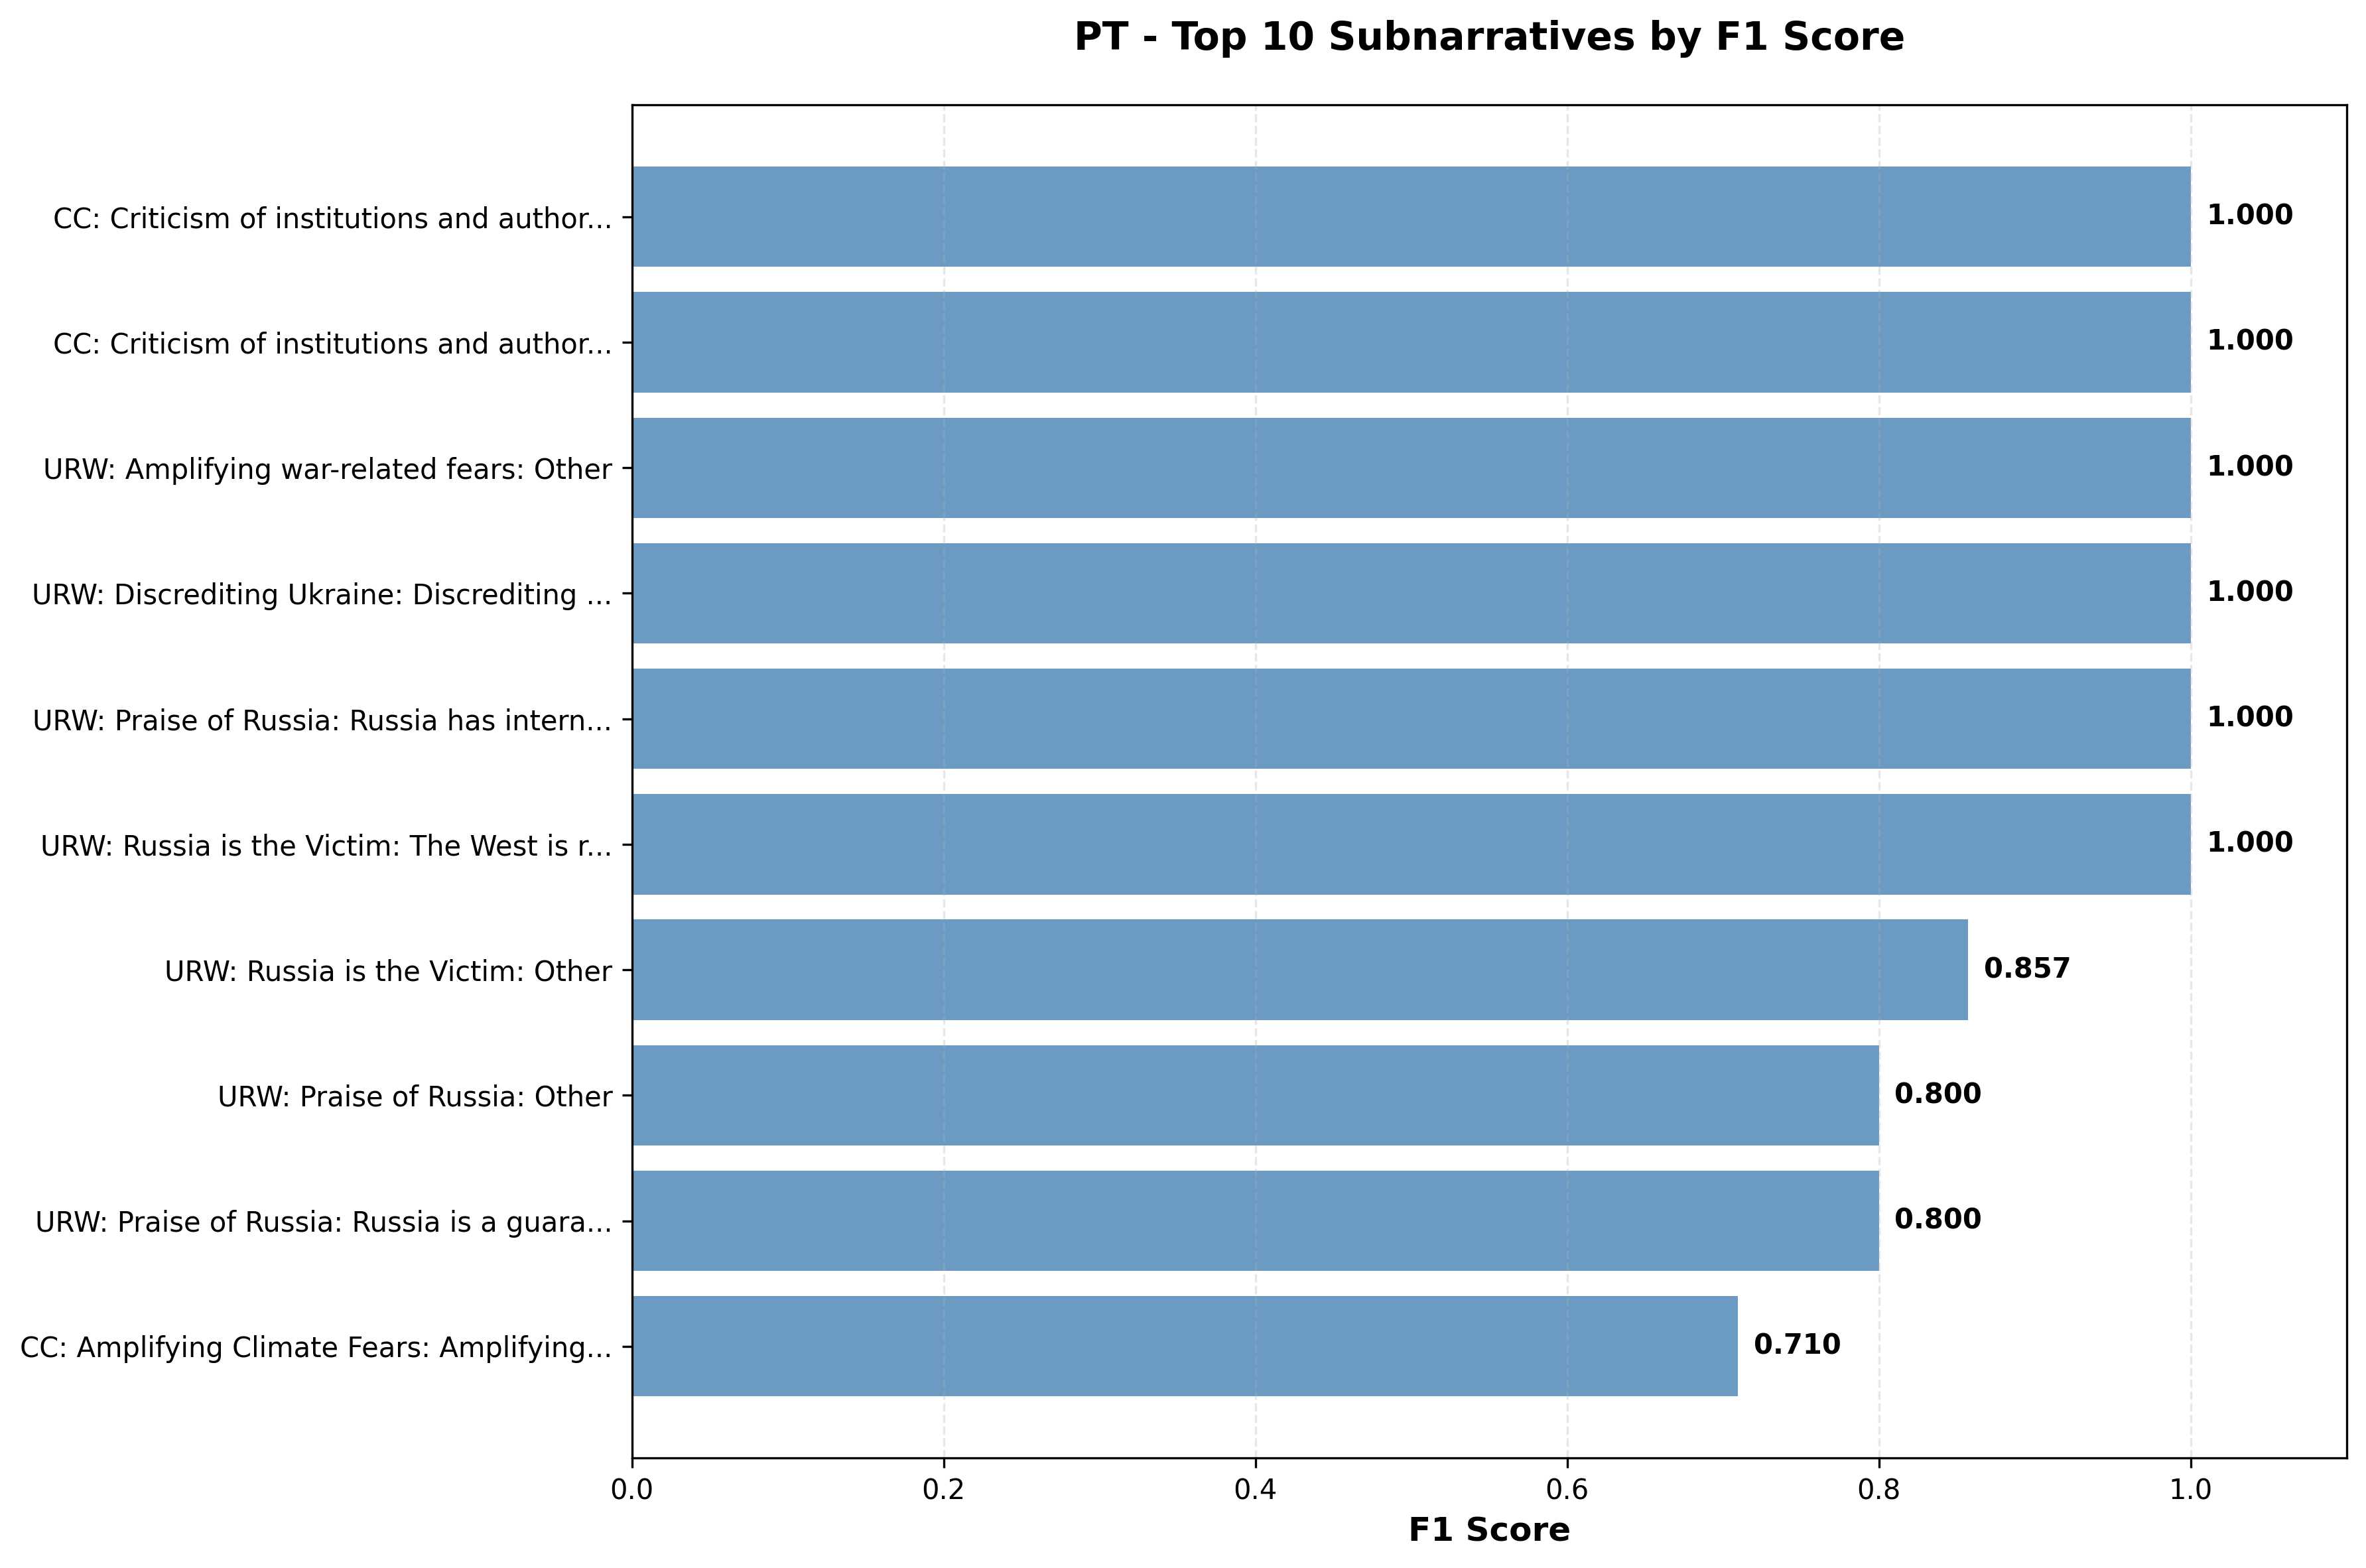
\includegraphics[width=\textwidth]{gemini25_flash_subnarr_val_evaluation/plots/PT_top_subnarratives_f1_scores.png}
        \caption{Top subnarrative F1 scores}
        \label{fig:app-subnarr-val-pt-subnarr}
    \end{subfigure}
    \caption{Portuguese performance breakdown for subnarrative-validation configuration.}
    \label{fig:app-subnarr-val-pt}
\end{figure}

\subsection{Russian (RU) Performance}

\begin{figure}[H]
    \centering
    \begin{subfigure}[b]{0.48\textwidth}
        \centering
        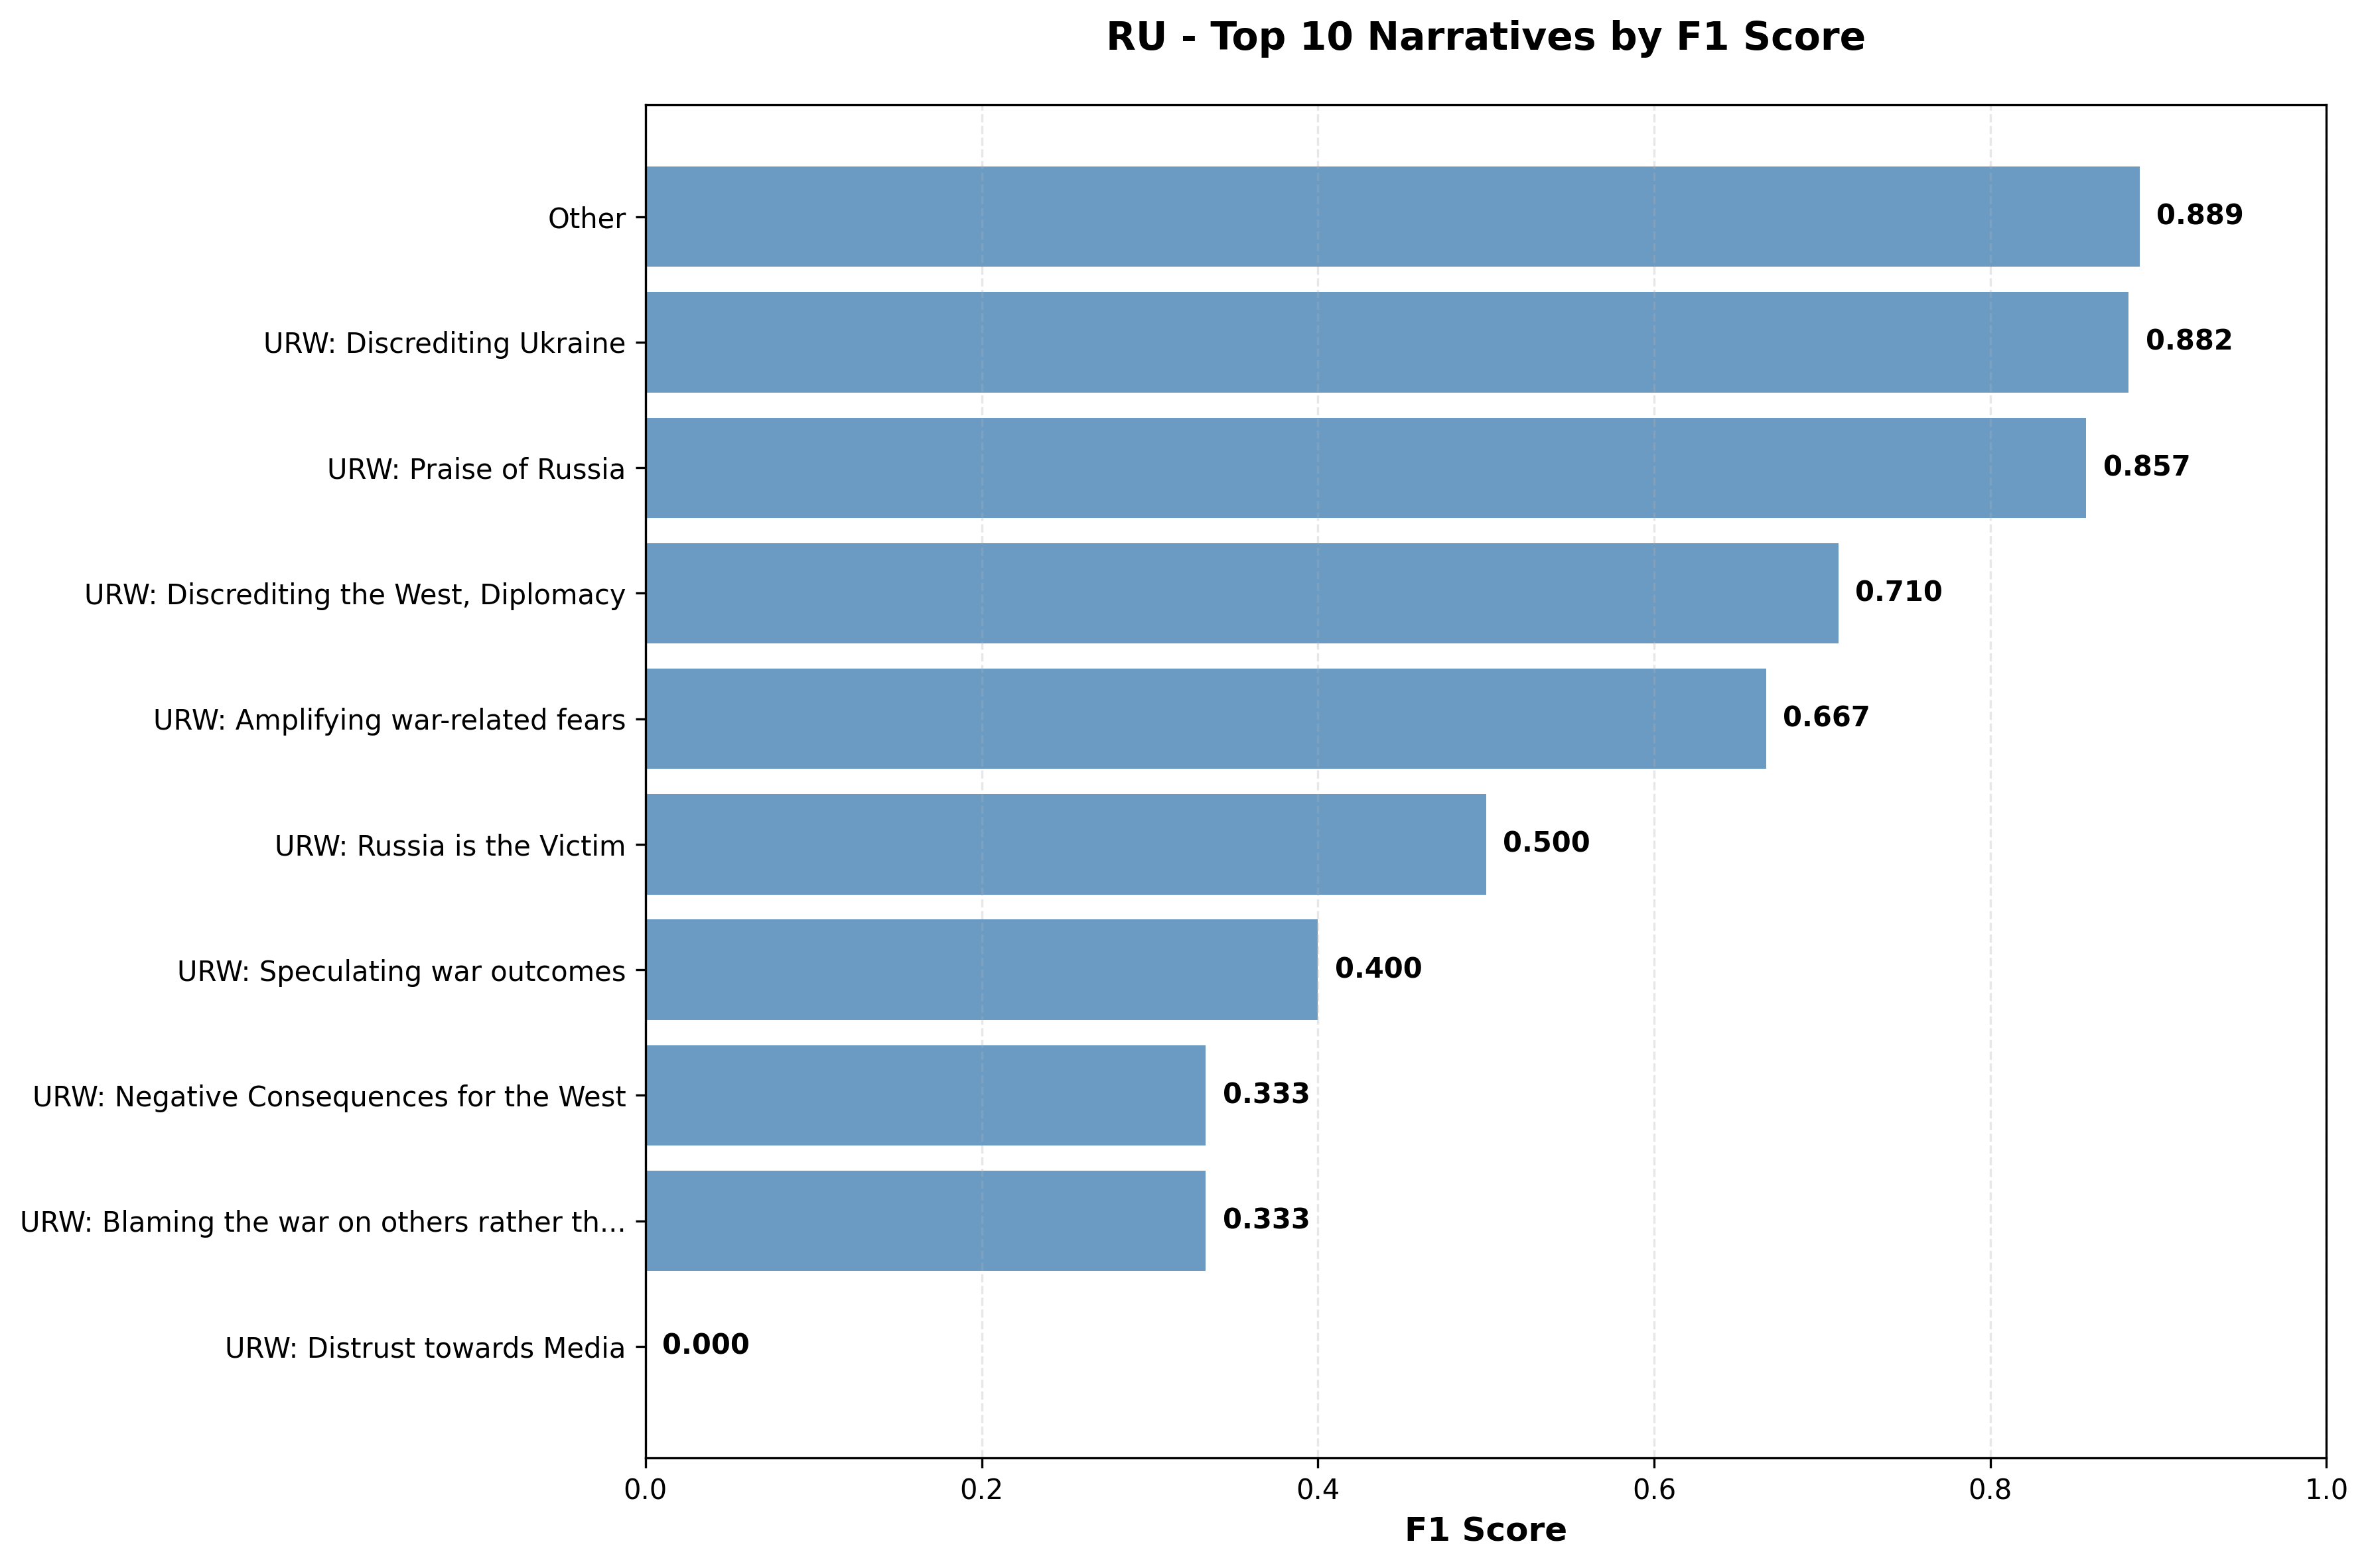
\includegraphics[width=\textwidth]{gemini25_flash_subnarr_val_evaluation/plots/RU_top_narratives_f1_scores.png}
        \caption{Top narrative F1 scores}
        \label{fig:app-subnarr-val-ru-narr}
    \end{subfigure}
    \hfill
    \begin{subfigure}[b]{0.48\textwidth}
        \centering
        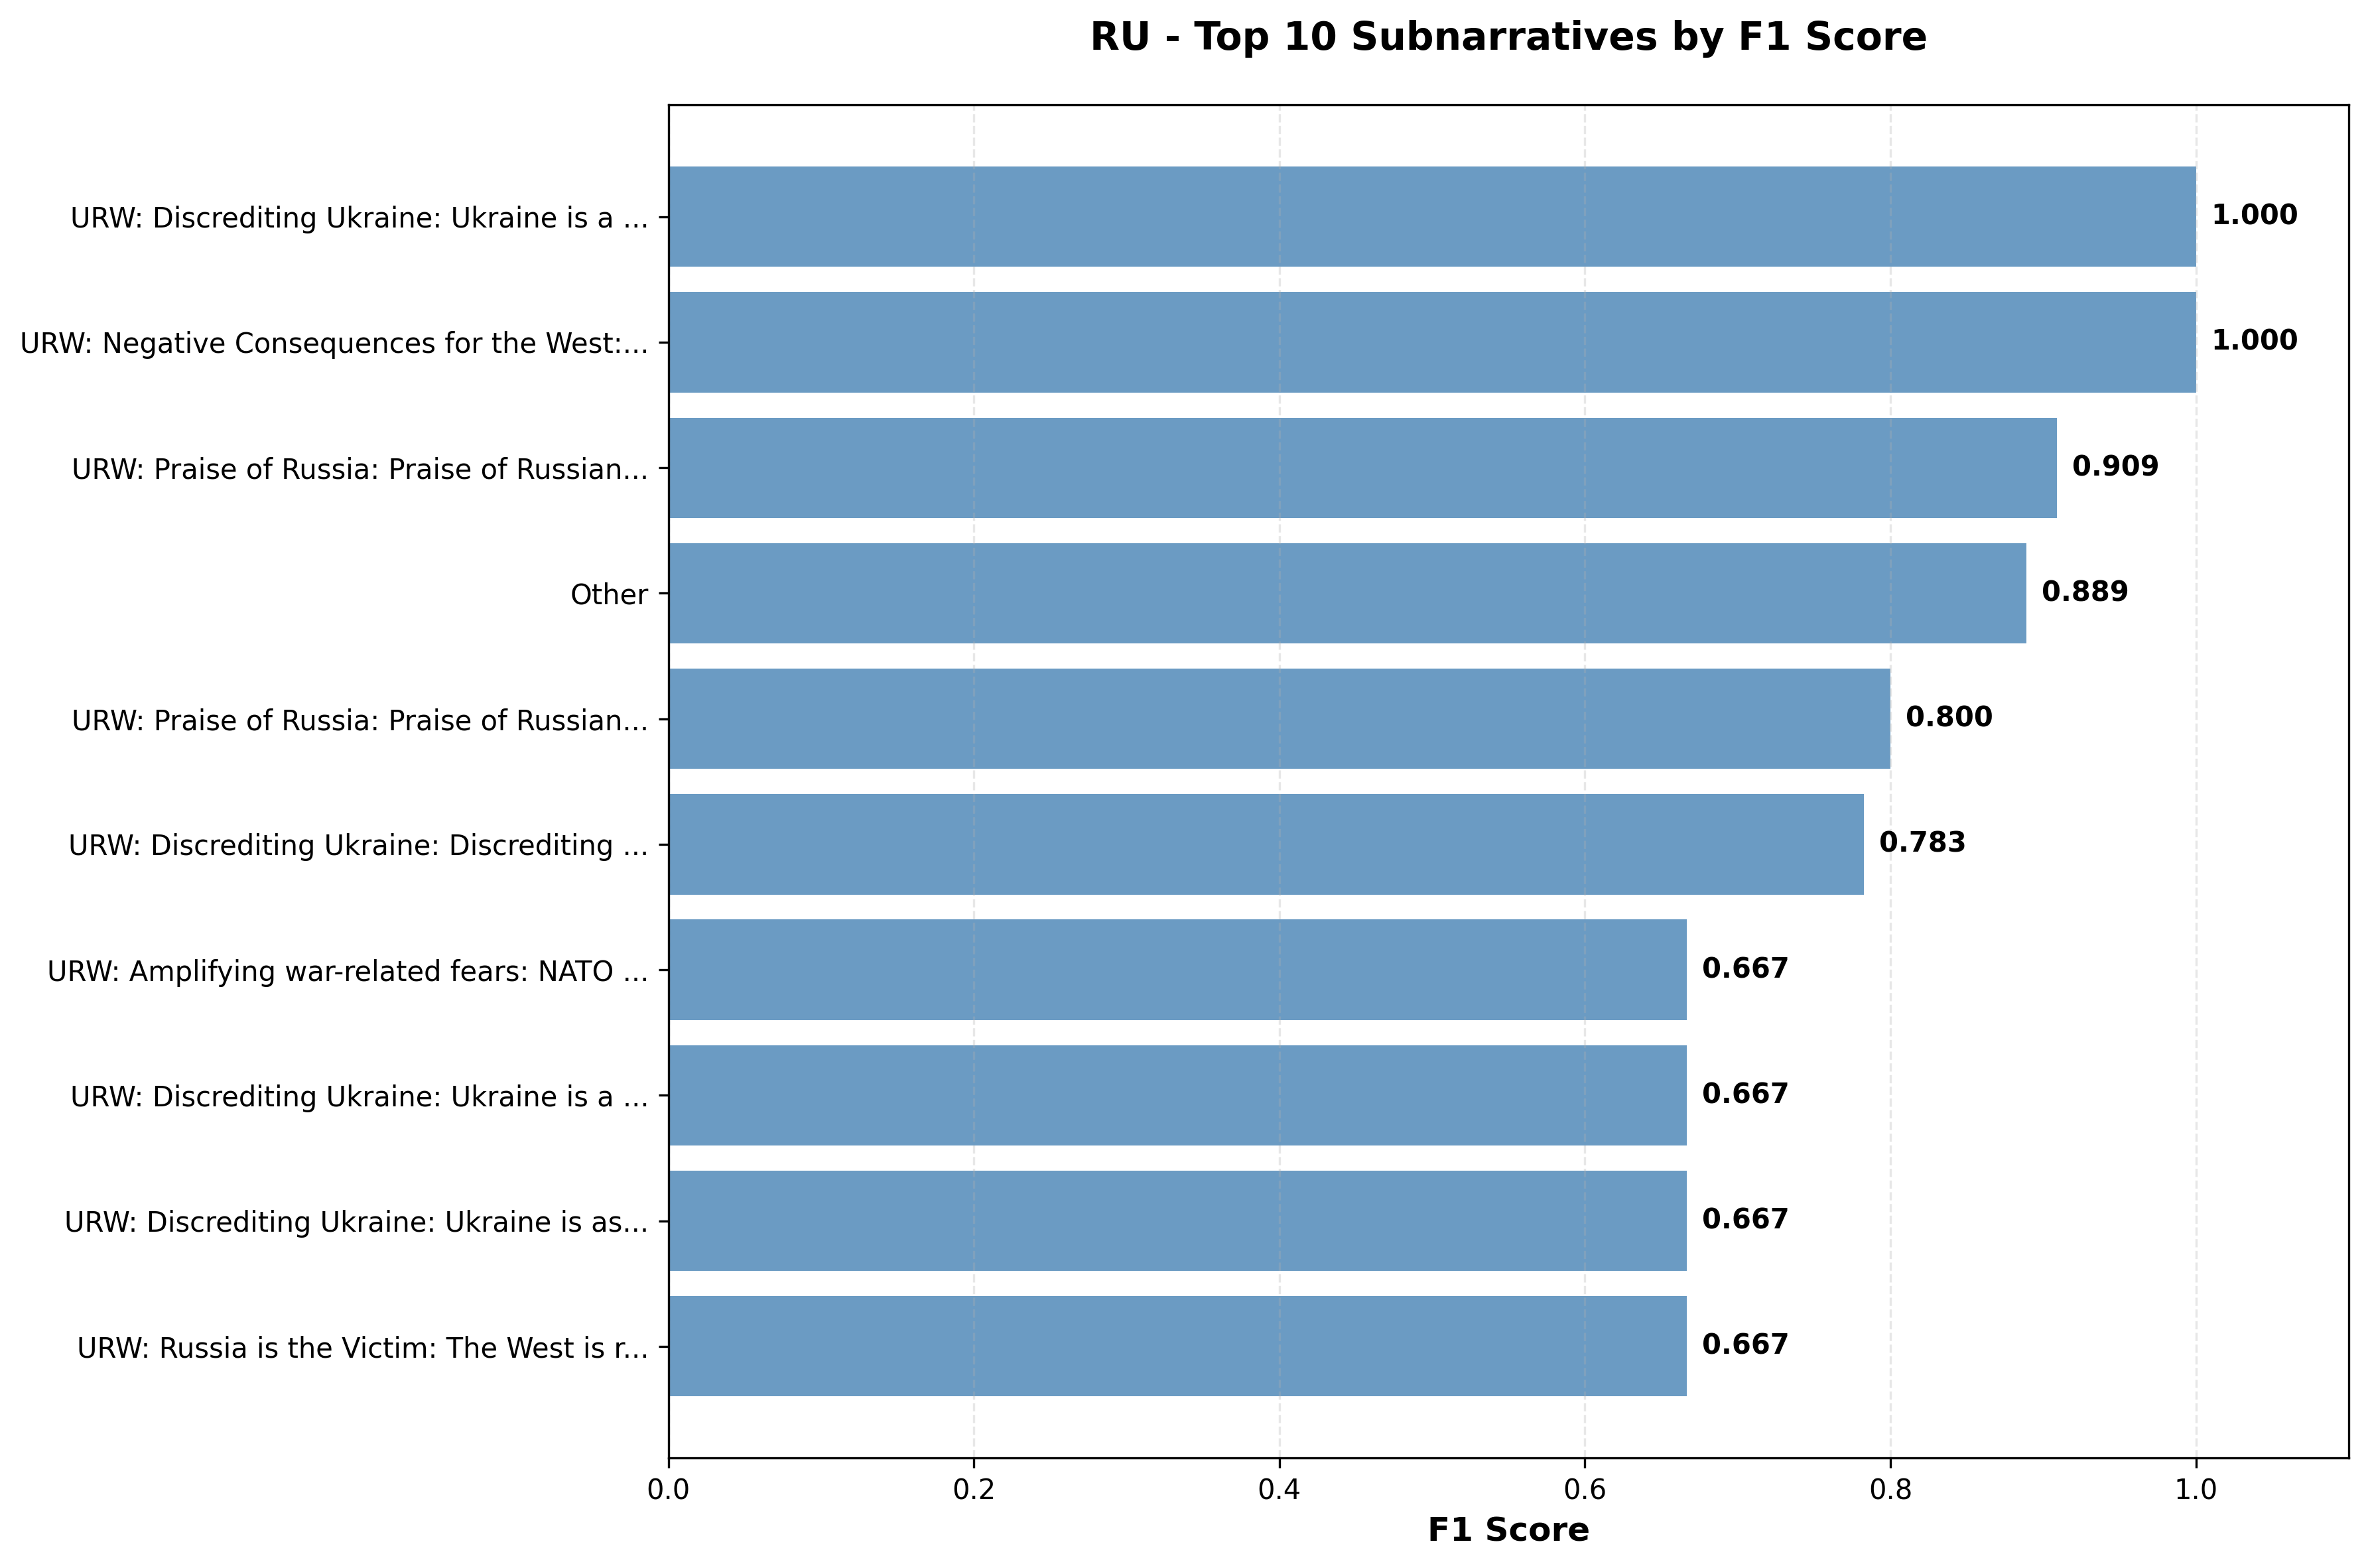
\includegraphics[width=\textwidth]{gemini25_flash_subnarr_val_evaluation/plots/RU_top_subnarratives_f1_scores.png}
        \caption{Top subnarrative F1 scores}
        \label{fig:app-subnarr-val-ru-subnarr}
    \end{subfigure}
    \caption{Russian performance breakdown for subnarrative-validation configuration.}
    \label{fig:app-subnarr-val-ru}
\end{figure}

\clearpage
\section{Confusion Matrices}
\label{app:confusion-matrices}

This section provides detailed confusion matrices for all evaluated configurations. Confusion matrices show the distribution of true positives (TP), false positives (FP), false negatives (FN), and true negatives (TN) for each label, enabling fine-grained error analysis.

\subsection{No-Validation Configuration Confusion Matrices}
\label{app:confusion-no-val}

The following confusion matrices correspond to the Actor-Critique pipeline without validation enabled. Complete per-label confusion matrices for all languages (BG, EN, HI, PT, RU) at both narrative and subnarrative levels are provided below.

\paragraph{Performance Summary:}
\begin{table}[H]
\centering
\caption{Performance overview by language for no-validation configuration}
\label{tab:app-confusion-no-val-summary}
\small
\begin{tabular}{lccccc}
\hline
\textbf{Language} & \textbf{Files} & \textbf{F1 Coarse} & \textbf{F1 Sample} & \textbf{Narr. Labels} & \textbf{Subnarr. Labels} \\
\hline
BG & 35 & 0.5799 & 0.4104 & 21 & 71 \\
EN & 41 & 0.5132 & 0.3815 & 22 & 83 \\
HI & 35 & 0.4715 & 0.2976 & 13 & 46 \\
PT & 35 & 0.7489 & 0.4737 & 14 & 40 \\
RU & 32 & 0.6958 & 0.4754 & 11 & 41 \\
\hline
\end{tabular}
\end{table}

% Confusion matrices for No Validation
% Auto-generated from gemini_confusion_matrices.md


\subsubsection{BG - Narrative Level}

{\small
\setlength{\tabcolsep}{4pt}
\begin{longtable}{lrrrrrr}
\caption{Confusion matrix for BG Narratives (No Validation)}
\label{tab:confusion-no-validation-bg-narratives} \\
\toprule
\textbf{Label} & \textbf{F1} & \textbf{Support} & \textbf{TP} & \textbf{FP} & \textbf{FN} & \textbf{TN} \\
\midrule
\endfirsthead
\multicolumn{7}{c}%
{{Table \thetable\ continued from previous page}} \\
\toprule
\textbf{Label} & \textbf{F1} & \textbf{Support} & \textbf{TP} & \textbf{FP} & \textbf{FN} & \textbf{TN} \\
\midrule
\endhead
\midrule
\multicolumn{7}{r}{{Continued on next page}} \\
\endfoot
\bottomrule
\endlastfoot
CC: Amplifying Climate Fears & 0.900 & 9 & 9 & 2 & 0 & 24 \\
URW: Discrediting Ukraine & 0.833 & 5 & 5 & 2 & 0 & 28 \\
CC: Criticism of climate policies & 0.800 & 2 & 2 & 1 & 0 & 32 \\
URW: Praise of Russia & 0.800 & 2 & 2 & 1 & 0 & 32 \\
URW: Amplifying war-related fears & 0.769 & 5 & 5 & 3 & 0 & 27 \\
CC: Criticism of climate movement & 0.667 & 1 & 1 & 1 & 0 & 33 \\
CC: Criticism of institutions and authorities & 0.667 & 3 & 3 & 3 & 0 & 29 \\
CC: Hidden plots by secret schemes of powerful groups & 0.667 & 2 & 1 & 0 & 1 & 33 \\
CC: Downplaying climate change & 0.571 & 4 & 2 & 1 & 2 & 30 \\
URW: Discrediting the West, Diplomacy & 0.526 & 5 & 5 & 9 & 0 & 21 \\
URW: Negative Consequences for the West & 0.500 & 3 & 2 & 3 & 1 & 29 \\
URW: Russia is the Victim & 0.500 & 3 & 3 & 6 & 0 & 26 \\
Other & 0.444 & 6 & 2 & 1 & 4 & 28 \\
URW: Blaming the war on others rather than the inv... & 0.250 & 2 & 1 & 5 & 1 & 28 \\
CC: Controversy about green technologies & 0.000 & 0 & 0 & 2 & 0 & 33 \\
CC: Green policies are geopolitical instruments & 0.000 & 1 & 0 & 3 & 1 & 31 \\
CC: Questioning the measurements and science & 0.000 & 0 & 0 & 1 & 0 & 34 \\
URW: Distrust towards Media & 0.000 & 0 & 0 & 2 & 0 & 33 \\
URW: Hidden plots by secret schemes of powerful gr... & 0.000 & 0 & 0 & 4 & 0 & 31 \\
URW: Overpraising the West & 0.000 & 1 & 0 & 0 & 1 & 34 \\
URW: Speculating war outcomes & 0.000 & 0 & 0 & 7 & 0 & 28 \\
\end{longtable}
}


\subsubsection{EN - Narrative Level}

{\small
\setlength{\tabcolsep}{4pt}
\begin{longtable}{lrrrrrr}
\caption{Confusion matrix for EN Narratives (No Validation)}
\label{tab:confusion-no-validation-en-narratives} \\
\toprule
\textbf{Label} & \textbf{F1} & \textbf{Support} & \textbf{TP} & \textbf{FP} & \textbf{FN} & \textbf{TN} \\
\midrule
\endfirsthead
\multicolumn{7}{c}%
{{Table \thetable\ continued from previous page}} \\
\toprule
\textbf{Label} & \textbf{F1} & \textbf{Support} & \textbf{TP} & \textbf{FP} & \textbf{FN} & \textbf{TN} \\
\midrule
\endhead
\midrule
\multicolumn{7}{r}{{Continued on next page}} \\
\endfoot
\bottomrule
\endlastfoot
URW: Overpraising the West & 1.000 & 1 & 1 & 0 & 0 & 40 \\
URW: Distrust towards Media & 0.889 & 4 & 4 & 1 & 0 & 36 \\
URW: Discrediting Ukraine & 0.875 & 7 & 7 & 2 & 0 & 32 \\
CC: Green policies are geopolitical instruments & 0.857 & 3 & 3 & 1 & 0 & 37 \\
CC: Questioning the measurements and science & 0.857 & 4 & 3 & 0 & 1 & 37 \\
URW: Blaming the war on others rather than the inv... & 0.857 & 6 & 6 & 2 & 0 & 33 \\
URW: Discrediting the West, Diplomacy & 0.842 & 9 & 8 & 2 & 1 & 30 \\
CC: Climate change is beneficial & 0.667 & 1 & 1 & 1 & 0 & 39 \\
CC: Hidden plots by secret schemes of powerful groups & 0.667 & 4 & 2 & 0 & 2 & 37 \\
URW: Praise of Russia & 0.571 & 2 & 2 & 3 & 0 & 36 \\
CC: Criticism of climate movement & 0.571 & 8 & 6 & 7 & 2 & 26 \\
URW: Speculating war outcomes & 0.500 & 4 & 4 & 8 & 0 & 29 \\
CC: Criticism of institutions and authorities & 0.476 & 8 & 5 & 8 & 3 & 25 \\
Other & 0.471 & 11 & 4 & 2 & 7 & 28 \\
URW: Amplifying war-related fears & 0.462 & 3 & 3 & 7 & 0 & 31 \\
CC: Downplaying climate change & 0.444 & 2 & 2 & 5 & 0 & 34 \\
CC: Criticism of climate policies & 0.333 & 3 & 3 & 12 & 0 & 26 \\
CC: Controversy about green technologies & 0.286 & 2 & 1 & 4 & 1 & 35 \\
URW: Russia is the Victim & 0.250 & 2 & 1 & 5 & 1 & 34 \\
CC: Amplifying Climate Fears & 0.000 & 0 & 0 & 2 & 0 & 39 \\
URW: Hidden plots by secret schemes of powerful gr... & 0.000 & 0 & 0 & 2 & 0 & 39 \\
URW: Negative Consequences for the West & 0.000 & 1 & 0 & 6 & 1 & 34 \\
\end{longtable}
}


\subsubsection{HI - Narrative Level}

{\small
\setlength{\tabcolsep}{4pt}
\begin{longtable}{lrrrrrr}
\caption{Confusion matrix for HI Narratives (No Validation)}
\label{tab:confusion-no-validation-hi-narratives} \\
\toprule
\textbf{Label} & \textbf{F1} & \textbf{Support} & \textbf{TP} & \textbf{FP} & \textbf{FN} & \textbf{TN} \\
\midrule
\endfirsthead
\multicolumn{7}{c}%
{{Table \thetable\ continued from previous page}} \\
\toprule
\textbf{Label} & \textbf{F1} & \textbf{Support} & \textbf{TP} & \textbf{FP} & \textbf{FN} & \textbf{TN} \\
\midrule
\endhead
\midrule
\multicolumn{7}{r}{{Continued on next page}} \\
\endfoot
\bottomrule
\endlastfoot
CC: Amplifying Climate Fears & 0.857 & 4 & 3 & 0 & 1 & 31 \\
URW: Amplifying war-related fears & 0.778 & 8 & 7 & 3 & 1 & 24 \\
URW: Praise of Russia & 0.667 & 13 & 8 & 3 & 5 & 19 \\
URW: Discrediting the West, Diplomacy & 0.609 & 7 & 7 & 9 & 0 & 19 \\
URW: Distrust towards Media & 0.500 & 2 & 1 & 1 & 1 & 32 \\
URW: Russia is the Victim & 0.421 & 9 & 4 & 6 & 5 & 20 \\
URW: Blaming the war on others rather than the inv... & 0.375 & 5 & 3 & 8 & 2 & 22 \\
Other & 0.286 & 2 & 1 & 4 & 1 & 29 \\
URW: Speculating war outcomes & 0.267 & 5 & 2 & 8 & 3 & 22 \\
URW: Discrediting Ukraine & 0.222 & 3 & 1 & 5 & 2 & 27 \\
URW: Negative Consequences for the West & 0.182 & 3 & 1 & 7 & 2 & 25 \\
URW: Hidden plots by secret schemes of powerful gr... & 0.000 & 2 & 0 & 0 & 2 & 33 \\
URW: Overpraising the West & 0.000 & 2 & 0 & 0 & 2 & 33 \\
\end{longtable}
}


\subsubsection{PT - Narrative Level}

{\small
\setlength{\tabcolsep}{4pt}
\begin{longtable}{lrrrrrr}
\caption{Confusion matrix for PT Narratives (No Validation)}
\label{tab:confusion-no-validation-pt-narratives} \\
\toprule
\textbf{Label} & \textbf{F1} & \textbf{Support} & \textbf{TP} & \textbf{FP} & \textbf{FN} & \textbf{TN} \\
\midrule
\endfirsthead
\multicolumn{7}{c}%
{{Table \thetable\ continued from previous page}} \\
\toprule
\textbf{Label} & \textbf{F1} & \textbf{Support} & \textbf{TP} & \textbf{FP} & \textbf{FN} & \textbf{TN} \\
\midrule
\endhead
\midrule
\multicolumn{7}{r}{{Continued on next page}} \\
\endfoot
\bottomrule
\endlastfoot
CC: Amplifying Climate Fears & 0.878 & 23 & 18 & 0 & 5 & 12 \\
URW: Discrediting the West, Diplomacy & 0.875 & 8 & 7 & 1 & 1 & 26 \\
URW: Praise of Russia & 0.857 & 4 & 3 & 0 & 1 & 31 \\
URW: Discrediting Ukraine & 0.800 & 3 & 2 & 0 & 1 & 32 \\
CC: Criticism of climate policies & 0.714 & 9 & 5 & 0 & 4 & 26 \\
CC: Criticism of institutions and authorities & 0.700 & 8 & 7 & 5 & 1 & 22 \\
URW: Negative Consequences for the West & 0.667 & 1 & 1 & 1 & 0 & 33 \\
URW: Russia is the Victim & 0.667 & 3 & 3 & 3 & 0 & 29 \\
Other & 0.500 & 1 & 1 & 2 & 0 & 32 \\
CC: Controversy about green technologies & 0.000 & 0 & 0 & 1 & 0 & 34 \\
CC: Green policies are geopolitical instruments & 0.000 & 0 & 0 & 2 & 0 & 33 \\
CC: Hidden plots by secret schemes of powerful groups & 0.000 & 1 & 0 & 0 & 1 & 34 \\
URW: Amplifying war-related fears & 0.000 & 1 & 0 & 0 & 1 & 34 \\
URW: Blaming the war on others rather than the inv... & 0.000 & 0 & 0 & 2 & 0 & 33 \\
\end{longtable}
}


\subsubsection{RU - Narrative Level}

{\small
\setlength{\tabcolsep}{4pt}
\begin{longtable}{lrrrrrr}
\caption{Confusion matrix for RU Narratives (No Validation)}
\label{tab:confusion-no-validation-ru-narratives} \\
\toprule
\textbf{Label} & \textbf{F1} & \textbf{Support} & \textbf{TP} & \textbf{FP} & \textbf{FN} & \textbf{TN} \\
\midrule
\endfirsthead
\multicolumn{7}{c}%
{{Table \thetable\ continued from previous page}} \\
\toprule
\textbf{Label} & \textbf{F1} & \textbf{Support} & \textbf{TP} & \textbf{FP} & \textbf{FN} & \textbf{TN} \\
\midrule
\endhead
\midrule
\multicolumn{7}{r}{{Continued on next page}} \\
\endfoot
\bottomrule
\endlastfoot
Other & 1.000 & 4 & 4 & 0 & 0 & 28 \\
URW: Discrediting Ukraine & 0.857 & 15 & 15 & 5 & 0 & 12 \\
URW: Discrediting the West, Diplomacy & 0.824 & 15 & 14 & 5 & 1 & 12 \\
URW: Praise of Russia & 0.815 & 15 & 11 & 1 & 4 & 16 \\
URW: Amplifying war-related fears & 0.667 & 2 & 2 & 2 & 0 & 28 \\
URW: Speculating war outcomes & 0.462 & 3 & 3 & 7 & 0 & 22 \\
URW: Russia is the Victim & 0.444 & 3 & 2 & 4 & 1 & 25 \\
URW: Negative Consequences for the West & 0.333 & 1 & 1 & 4 & 0 & 27 \\
URW: Blaming the war on others rather than the inv... & 0.333 & 4 & 2 & 6 & 2 & 22 \\
URW: Distrust towards Media & 0.000 & 2 & 0 & 1 & 2 & 29 \\
URW: Hidden plots by secret schemes of powerful gr... & 0.000 & 1 & 0 & 3 & 1 & 28 \\
\end{longtable}
}


\subsubsection{BG - Subnarrative Level}

{\small
\setlength{\tabcolsep}{4pt}
\begin{longtable}{lrrrrrr}
\caption{Confusion matrix for BG Subnarratives (No Validation)}
\label{tab:confusion-no-validation-bg-subnarratives} \\
\toprule
\textbf{Label} & \textbf{F1} & \textbf{Support} & \textbf{TP} & \textbf{FP} & \textbf{FN} & \textbf{TN} \\
\midrule
\endfirsthead
\multicolumn{7}{c}%
{{Table \thetable\ continued from previous page}} \\
\toprule
\textbf{Label} & \textbf{F1} & \textbf{Support} & \textbf{TP} & \textbf{FP} & \textbf{FN} & \textbf{TN} \\
\midrule
\endhead
\midrule
\multicolumn{7}{r}{{Continued on next page}} \\
\endfoot
\bottomrule
\endlastfoot
CC: Criticism of climate movement: Ad hominem atta... & 1.000 & 1 & 1 & 0 & 0 & 34 \\
CC: Criticism of climate policies: Climate policie... & 1.000 & 1 & 1 & 0 & 0 & 34 \\
CC: Downplaying climate change: Climate cycles are... & 1.000 & 1 & 1 & 0 & 0 & 34 \\
CC: Hidden plots by secret schemes of powerful gro... & 1.000 & 1 & 1 & 0 & 0 & 34 \\
CC: Hidden plots by secret schemes of powerful gro... & 1.000 & 1 & 1 & 0 & 0 & 34 \\
URW: Amplifying war-related fears: There is a real... & 1.000 & 2 & 2 & 0 & 0 & 33 \\
URW: Praise of Russia: Praise of Russian President... & 1.000 & 1 & 1 & 0 & 0 & 34 \\
CC: Amplifying Climate Fears: Amplifying existing ... & 0.900 & 9 & 9 & 2 & 0 & 24 \\
CC: Criticism of climate movement: Climate movemen... & 0.667 & 1 & 1 & 1 & 0 & 33 \\
CC: Criticism of climate movement: Other & 0.667 & 1 & 1 & 1 & 0 & 33 \\
CC: Criticism of climate policies: Climate policie... & 0.667 & 1 & 1 & 1 & 0 & 33 \\
CC: Criticism of institutions and authorities: Cri... & 0.667 & 2 & 2 & 2 & 0 & 31 \\
URW: Amplifying war-related fears: By continuing t... & 0.667 & 1 & 1 & 1 & 0 & 33 \\
URW: Praise of Russia: Praise of Russian military ... & 0.667 & 1 & 1 & 1 & 0 & 33 \\
URW: Praise of Russia: Russia has international su... & 0.667 & 1 & 1 & 1 & 0 & 33 \\
URW: Russia is the Victim: The West is russophobic & 0.600 & 3 & 3 & 4 & 0 & 28 \\
URW: Discrediting Ukraine: Discrediting Ukrainian ... & 0.571 & 2 & 2 & 3 & 0 & 30 \\
URW: Discrediting the West, Diplomacy: Other & 0.500 & 5 & 4 & 7 & 1 & 23 \\
CC: Downplaying climate change: Weather suggests t... & 0.500 & 3 & 1 & 0 & 2 & 32 \\
URW: Amplifying war-related fears: Other & 0.500 & 2 & 2 & 4 & 0 & 29 \\
URW: Amplifying war-related fears: Russia will als... & 0.500 & 1 & 1 & 2 & 0 & 32 \\
URW: Discrediting Ukraine: Ukraine is a hub for cr... & 0.500 & 1 & 1 & 2 & 0 & 32 \\
URW: Discrediting Ukraine: Ukraine is a puppet of ... & 0.500 & 2 & 2 & 4 & 0 & 29 \\
URW: Discrediting Ukraine: Ukraine is associated w... & 0.500 & 1 & 1 & 2 & 0 & 32 \\
URW: Negative Consequences for the West: Other & 0.500 & 3 & 2 & 3 & 1 & 29 \\
Other & 0.444 & 6 & 2 & 1 & 4 & 28 \\
CC: Criticism of institutions and authorities: Cri... & 0.400 & 1 & 1 & 3 & 0 & 31 \\
URW: Blaming the war on others rather than the inv... & 0.400 & 1 & 1 & 3 & 0 & 31 \\
CC: Amplifying Climate Fears: Doomsday scenarios f... & 0.364 & 2 & 2 & 7 & 0 & 26 \\
URW: Discrediting Ukraine: Discrediting Ukrainian ... & 0.333 & 1 & 1 & 4 & 0 & 30 \\
CC: Amplifying Climate Fears: Other & 0.333 & 4 & 1 & 1 & 3 & 30 \\
CC: Amplifying Climate Fears: Earth will be uninha... & 0.000 & 0 & 0 & 2 & 0 & 33 \\
CC: Controversy about green technologies: Other & 0.000 & 0 & 0 & 1 & 0 & 34 \\
CC: Controversy about green technologies: Renewabl... & 0.000 & 0 & 0 & 1 & 0 & 34 \\
CC: Controversy about green technologies: Renewabl... & 0.000 & 0 & 0 & 2 & 0 & 33 \\
CC: Criticism of climate movement: Climate movemen... & 0.000 & 0 & 0 & 2 & 0 & 33 \\
CC: Criticism of climate policies: Climate policie... & 0.000 & 0 & 0 & 1 & 0 & 34 \\
CC: Criticism of climate policies: Other & 0.000 & 0 & 0 & 3 & 0 & 32 \\
CC: Criticism of institutions and authorities: Cri... & 0.000 & 0 & 0 & 2 & 0 & 33 \\
CC: Criticism of institutions and authorities: Cri... & 0.000 & 0 & 0 & 1 & 0 & 34 \\
CC: Criticism of institutions and authorities: Other & 0.000 & 0 & 0 & 2 & 0 & 33 \\
CC: Downplaying climate change: Human activities d... & 0.000 & 0 & 0 & 1 & 0 & 34 \\
CC: Downplaying climate change: Other & 0.000 & 0 & 0 & 3 & 0 & 32 \\
CC: Green policies are geopolitical instruments: C... & 0.000 & 0 & 0 & 2 & 0 & 33 \\
CC: Green policies are geopolitical instruments: G... & 0.000 & 1 & 0 & 1 & 1 & 33 \\
CC: Green policies are geopolitical instruments: O... & 0.000 & 0 & 0 & 2 & 0 & 33 \\
CC: Hidden plots by secret schemes of powerful gro... & 0.000 & 1 & 0 & 1 & 1 & 33 \\
CC: Questioning the measurements and science: Other & 0.000 & 0 & 0 & 1 & 0 & 34 \\
CC: Questioning the measurements and science: Scie... & 0.000 & 0 & 0 & 1 & 0 & 34 \\
URW: Amplifying war-related fears: NATO should/wil... & 0.000 & 0 & 0 & 1 & 0 & 34 \\
URW: Blaming the war on others rather than the inv... & 0.000 & 0 & 0 & 1 & 0 & 34 \\
URW: Blaming the war on others rather than the inv... & 0.000 & 1 & 0 & 6 & 1 & 28 \\
URW: Discrediting Ukraine: Discrediting Ukrainian ... & 0.000 & 0 & 0 & 4 & 0 & 31 \\
URW: Discrediting Ukraine: Other & 0.000 & 0 & 0 & 3 & 0 & 32 \\
URW: Discrediting Ukraine: Situation in Ukraine is... & 0.000 & 0 & 0 & 1 & 0 & 34 \\
URW: Discrediting the West, Diplomacy: Diplomacy d... & 0.000 & 0 & 0 & 3 & 0 & 32 \\
URW: Discrediting the West, Diplomacy: The EU is d... & 0.000 & 0 & 0 & 3 & 0 & 32 \\
URW: Discrediting the West, Diplomacy: The West do... & 0.000 & 0 & 0 & 4 & 0 & 31 \\
URW: Discrediting the West, Diplomacy: The West is... & 0.000 & 0 & 0 & 3 & 0 & 32 \\
URW: Discrediting the West, Diplomacy: The West is... & 0.000 & 0 & 0 & 6 & 0 & 29 \\
URW: Discrediting the West, Diplomacy: West is tir... & 0.000 & 0 & 0 & 1 & 0 & 34 \\
URW: Distrust towards Media: Ukrainian media canno... & 0.000 & 0 & 0 & 1 & 0 & 34 \\
URW: Distrust towards Media: Western media is an i... & 0.000 & 0 & 0 & 2 & 0 & 33 \\
URW: Hidden plots by secret schemes of powerful gr... & 0.000 & 0 & 0 & 4 & 0 & 31 \\
URW: Overpraising the West: The West belongs in th... & 0.000 & 1 & 0 & 0 & 1 & 34 \\
URW: Praise of Russia: Other & 0.000 & 0 & 0 & 2 & 0 & 33 \\
URW: Russia is the Victim: Other & 0.000 & 0 & 0 & 4 & 0 & 31 \\
URW: Russia is the Victim: Russia actions in Ukrai... & 0.000 & 0 & 0 & 5 & 0 & 30 \\
URW: Russia is the Victim: UA is anti-RU extremists & 0.000 & 0 & 0 & 3 & 0 & 32 \\
URW: Speculating war outcomes: Other & 0.000 & 0 & 0 & 6 & 0 & 29 \\
URW: Speculating war outcomes: Russian army is col... & 0.000 & 0 & 0 & 1 & 0 & 34 \\
\end{longtable}
}


\subsubsection{EN - Subnarrative Level}

{\small
\setlength{\tabcolsep}{4pt}
\begin{longtable}{lrrrrrr}
\caption{Confusion matrix for EN Subnarratives (No Validation)}
\label{tab:confusion-no-validation-en-subnarratives} \\
\toprule
\textbf{Label} & \textbf{F1} & \textbf{Support} & \textbf{TP} & \textbf{FP} & \textbf{FN} & \textbf{TN} \\
\midrule
\endfirsthead
\multicolumn{7}{c}%
{{Table \thetable\ continued from previous page}} \\
\toprule
\textbf{Label} & \textbf{F1} & \textbf{Support} & \textbf{TP} & \textbf{FP} & \textbf{FN} & \textbf{TN} \\
\midrule
\endhead
\midrule
\multicolumn{7}{r}{{Continued on next page}} \\
\endfoot
\bottomrule
\endlastfoot
CC: Climate change is beneficial: CO2 is beneficial & 1.000 & 1 & 1 & 0 & 0 & 40 \\
CC: Downplaying climate change: Human activities d... & 1.000 & 2 & 2 & 0 & 0 & 39 \\
URW: Discrediting the West, Diplomacy: The EU is d... & 1.000 & 1 & 1 & 0 & 0 & 40 \\
URW: Overpraising the West: The West belongs in th... & 1.000 & 1 & 1 & 0 & 0 & 40 \\
URW: Speculating war outcomes: Russian army is col... & 1.000 & 2 & 2 & 0 & 0 & 39 \\
URW: Blaming the war on others rather than the inv... & 0.857 & 6 & 6 & 2 & 0 & 33 \\
URW: Discrediting the West, Diplomacy: Other & 0.857 & 6 & 6 & 2 & 0 & 33 \\
URW: Discrediting Ukraine: Ukraine is associated w... & 0.800 & 2 & 2 & 1 & 0 & 38 \\
CC: Criticism of institutions and authorities: Cri... & 0.769 & 6 & 5 & 2 & 1 & 33 \\
URW: Distrust towards Media: Western media is an i... & 0.750 & 4 & 3 & 1 & 1 & 36 \\
CC: Controversy about green technologies: Renewabl... & 0.667 & 1 & 1 & 1 & 0 & 39 \\
CC: Criticism of climate movement: Climate movemen... & 0.667 & 4 & 4 & 4 & 0 & 33 \\
CC: Green policies are geopolitical instruments: C... & 0.667 & 2 & 2 & 2 & 0 & 37 \\
CC: Hidden plots by secret schemes of powerful gro... & 0.667 & 2 & 1 & 0 & 1 & 39 \\
CC: Questioning the measurements and science: Scie... & 0.667 & 1 & 1 & 1 & 0 & 39 \\
URW: Amplifying war-related fears: There is a real... & 0.667 & 2 & 2 & 2 & 0 & 37 \\
URW: Blaming the war on others rather than the inv... & 0.667 & 1 & 1 & 1 & 0 & 39 \\
URW: Discrediting Ukraine: Other & 0.667 & 1 & 1 & 1 & 0 & 39 \\
URW: Praise of Russia: Praise of Russian President... & 0.667 & 1 & 1 & 1 & 0 & 39 \\
URW: Praise of Russia: Russia is a guarantor of pe... & 0.667 & 1 & 1 & 1 & 0 & 39 \\
CC: Criticism of climate movement: Ad hominem atta... & 0.571 & 3 & 2 & 2 & 1 & 36 \\
URW: Discrediting Ukraine: Ukraine is a puppet of ... & 0.545 & 3 & 3 & 5 & 0 & 33 \\
CC: Criticism of climate policies: Climate policie... & 0.500 & 1 & 1 & 2 & 0 & 38 \\
CC: Green policies are geopolitical instruments: O... & 0.500 & 1 & 1 & 2 & 0 & 38 \\
URW: Discrediting Ukraine: Discrediting Ukrainian ... & 0.500 & 3 & 3 & 6 & 0 & 32 \\
URW: Discrediting Ukraine: Discrediting Ukrainian ... & 0.500 & 2 & 2 & 4 & 0 & 35 \\
URW: Discrediting the West, Diplomacy: Diplomacy d... & 0.500 & 3 & 2 & 3 & 1 & 35 \\
URW: Speculating war outcomes: Ukrainian army is c... & 0.500 & 2 & 2 & 4 & 0 & 35 \\
Other & 0.471 & 11 & 4 & 2 & 7 & 28 \\
URW: Discrediting the West, Diplomacy: The West do... & 0.462 & 4 & 3 & 6 & 1 & 31 \\
CC: Criticism of institutions and authorities: Cri... & 0.400 & 3 & 2 & 5 & 1 & 33 \\
CC: Criticism of institutions and authorities: Other & 0.400 & 1 & 1 & 3 & 0 & 37 \\
CC: Questioning the measurements and science: Meth... & 0.400 & 3 & 1 & 1 & 2 & 37 \\
URW: Amplifying war-related fears: By continuing t... & 0.400 & 1 & 1 & 3 & 0 & 37 \\
URW: Discrediting Ukraine: Discrediting Ukrainian ... & 0.400 & 1 & 1 & 3 & 0 & 37 \\
CC: Controversy about green technologies: Other & 0.333 & 1 & 1 & 4 & 0 & 36 \\
URW: Discrediting Ukraine: Situation in Ukraine is... & 0.333 & 1 & 1 & 4 & 0 & 36 \\
URW: Discrediting the West, Diplomacy: The West is... & 0.333 & 1 & 1 & 4 & 0 & 36 \\
URW: Praise of Russia: Praise of Russian military ... & 0.333 & 1 & 1 & 4 & 0 & 36 \\
CC: Criticism of climate movement: Climate movemen... & 0.333 & 3 & 1 & 2 & 2 & 36 \\
CC: Criticism of institutions and authorities: Cri... & 0.286 & 2 & 1 & 4 & 1 & 35 \\
CC: Downplaying climate change: Other & 0.286 & 1 & 1 & 5 & 0 & 35 \\
URW: Russia is the Victim: Other & 0.286 & 1 & 1 & 5 & 0 & 35 \\
CC: Criticism of climate movement: Other & 0.250 & 4 & 2 & 10 & 2 & 27 \\
CC: Criticism of climate policies: Climate policie... & 0.200 & 1 & 1 & 8 & 0 & 32 \\
CC: Criticism of climate policies: Other & 0.143 & 1 & 1 & 12 & 0 & 28 \\
CC: Amplifying Climate Fears: Amplifying existing ... & 0.000 & 0 & 0 & 2 & 0 & 39 \\
CC: Amplifying Climate Fears: Doomsday scenarios f... & 0.000 & 0 & 0 & 1 & 0 & 40 \\
CC: Climate change is beneficial: Temperature incr... & 0.000 & 0 & 0 & 1 & 0 & 40 \\
CC: Controversy about green technologies: Renewabl... & 0.000 & 1 & 0 & 4 & 1 & 36 \\
CC: Controversy about green technologies: Renewabl... & 0.000 & 0 & 0 & 2 & 0 & 39 \\
CC: Criticism of climate policies: Climate policie... & 0.000 & 0 & 0 & 9 & 0 & 32 \\
CC: Criticism of institutions and authorities: Cri... & 0.000 & 0 & 0 & 1 & 0 & 40 \\
CC: Downplaying climate change: CO2 concentrations... & 0.000 & 0 & 0 & 2 & 0 & 39 \\
CC: Downplaying climate change: Ice is not melting & 0.000 & 0 & 0 & 1 & 0 & 40 \\
CC: Downplaying climate change: Temperature increa... & 0.000 & 0 & 0 & 3 & 0 & 38 \\
CC: Hidden plots by secret schemes of powerful gro... & 0.000 & 1 & 0 & 2 & 1 & 38 \\
CC: Hidden plots by secret schemes of powerful gro... & 0.000 & 1 & 0 & 0 & 1 & 40 \\
CC: Questioning the measurements and science: Data... & 0.000 & 1 & 0 & 0 & 1 & 40 \\
CC: Questioning the measurements and science: Gree... & 0.000 & 0 & 0 & 1 & 0 & 40 \\
CC: Questioning the measurements and science: Other & 0.000 & 0 & 0 & 1 & 0 & 40 \\
URW: Amplifying war-related fears: NATO should/wil... & 0.000 & 0 & 0 & 2 & 0 & 39 \\
URW: Amplifying war-related fears: Other & 0.000 & 0 & 0 & 8 & 0 & 33 \\
URW: Amplifying war-related fears: Russia will als... & 0.000 & 0 & 0 & 3 & 0 & 38 \\
URW: Blaming the war on others rather than the inv... & 0.000 & 0 & 0 & 4 & 0 & 37 \\
URW: Discrediting Ukraine: Rewriting Ukraine’s his... & 0.000 & 0 & 0 & 2 & 0 & 39 \\
URW: Discrediting Ukraine: Ukraine is a hub for cr... & 0.000 & 1 & 0 & 0 & 1 & 40 \\
URW: Discrediting the West, Diplomacy: The West is... & 0.000 & 0 & 0 & 2 & 0 & 39 \\
URW: Discrediting the West, Diplomacy: West is tir... & 0.000 & 0 & 0 & 1 & 0 & 40 \\
URW: Distrust towards Media: Other & 0.000 & 0 & 0 & 1 & 0 & 40 \\
URW: Distrust towards Media: Ukrainian media canno... & 0.000 & 0 & 0 & 1 & 0 & 40 \\
URW: Hidden plots by secret schemes of powerful gr... & 0.000 & 0 & 0 & 2 & 0 & 39 \\
URW: Negative Consequences for the West: Other & 0.000 & 0 & 0 & 6 & 0 & 35 \\
URW: Negative Consequences for the West: Sanctions... & 0.000 & 1 & 0 & 1 & 1 & 39 \\
URW: Overpraising the West: NATO will destroy Russia & 0.000 & 0 & 0 & 1 & 0 & 40 \\
URW: Overpraising the West: The West has the stron... & 0.000 & 0 & 0 & 1 & 0 & 40 \\
URW: Praise of Russia: Other & 0.000 & 1 & 0 & 3 & 1 & 37 \\
URW: Praise of Russia: Russian invasion has strong... & 0.000 & 0 & 0 & 2 & 0 & 39 \\
URW: Russia is the Victim: Russia actions in Ukrai... & 0.000 & 0 & 0 & 5 & 0 & 36 \\
URW: Russia is the Victim: The West is russophobic & 0.000 & 1 & 0 & 3 & 1 & 37 \\
URW: Russia is the Victim: UA is anti-RU extremists & 0.000 & 0 & 0 & 1 & 0 & 40 \\
URW: Speculating war outcomes: Other & 0.000 & 0 & 0 & 9 & 0 & 32 \\
URW: Speculating war outcomes: Russian army will l... & 0.000 & 0 & 0 & 1 & 0 & 40 \\
\end{longtable}
}


\subsubsection{HI - Subnarrative Level}

{\small
\setlength{\tabcolsep}{4pt}
\begin{longtable}{lrrrrrr}
\caption{Confusion matrix for HI Subnarratives (No Validation)}
\label{tab:confusion-no-validation-hi-subnarratives} \\
\toprule
\textbf{Label} & \textbf{F1} & \textbf{Support} & \textbf{TP} & \textbf{FP} & \textbf{FN} & \textbf{TN} \\
\midrule
\endfirsthead
\multicolumn{7}{c}%
{{Table \thetable\ continued from previous page}} \\
\toprule
\textbf{Label} & \textbf{F1} & \textbf{Support} & \textbf{TP} & \textbf{FP} & \textbf{FN} & \textbf{TN} \\
\midrule
\endhead
\midrule
\multicolumn{7}{r}{{Continued on next page}} \\
\endfoot
\bottomrule
\endlastfoot
URW: Amplifying war-related fears: There is a real... & 1.000 & 5 & 5 & 0 & 0 & 30 \\
URW: Distrust towards Media: Western media is an i... & 1.000 & 1 & 1 & 0 & 0 & 34 \\
CC: Amplifying Climate Fears: Amplifying existing ... & 0.857 & 4 & 3 & 0 & 1 & 31 \\
URW: Amplifying war-related fears: By continuing t... & 0.750 & 3 & 3 & 2 & 0 & 30 \\
URW: Discrediting the West, Diplomacy: West is tir... & 0.667 & 2 & 1 & 0 & 1 & 33 \\
URW: Amplifying war-related fears: Russia will als... & 0.571 & 4 & 2 & 1 & 2 & 30 \\
URW: Discrediting Ukraine: Ukraine is a puppet of ... & 0.500 & 1 & 1 & 2 & 0 & 32 \\
URW: Discrediting the West, Diplomacy: The West is... & 0.500 & 2 & 1 & 1 & 1 & 32 \\
URW: Speculating war outcomes: Ukrainian army is c... & 0.500 & 1 & 1 & 2 & 0 & 32 \\
URW: Praise of Russia: Russia has international su... & 0.471 & 10 & 4 & 3 & 6 & 22 \\
URW: Praise of Russia: Praise of Russian military ... & 0.462 & 3 & 3 & 7 & 0 & 25 \\
URW: Negative Consequences for the West: Sanctions... & 0.400 & 3 & 1 & 1 & 2 & 31 \\
URW: Russia is the Victim: Russia actions in Ukrai... & 0.364 & 2 & 2 & 7 & 0 & 26 \\
URW: Discrediting Ukraine: Discrediting Ukrainian ... & 0.333 & 3 & 1 & 2 & 2 & 30 \\
URW: Blaming the war on others rather than the inv... & 0.308 & 3 & 2 & 8 & 1 & 24 \\
Other & 0.286 & 2 & 1 & 4 & 1 & 29 \\
URW: Blaming the war on others rather than the inv... & 0.286 & 2 & 1 & 4 & 1 & 29 \\
URW: Discrediting the West, Diplomacy: Other & 0.286 & 3 & 2 & 9 & 1 & 23 \\
URW: Praise of Russia: Praise of Russian President... & 0.286 & 1 & 1 & 5 & 0 & 29 \\
URW: Discrediting the West, Diplomacy: The West is... & 0.250 & 1 & 1 & 6 & 0 & 28 \\
URW: Praise of Russia: Russia is a guarantor of pe... & 0.250 & 3 & 1 & 4 & 2 & 28 \\
URW: Discrediting the West, Diplomacy: The West do... & 0.222 & 3 & 1 & 5 & 2 & 27 \\
URW: Russia is the Victim: The West is russophobic & 0.200 & 7 & 1 & 2 & 6 & 26 \\
URW: Speculating war outcomes: Other & 0.182 & 2 & 1 & 8 & 1 & 25 \\
CC: Amplifying Climate Fears: Doomsday scenarios f... & 0.000 & 0 & 0 & 2 & 0 & 33 \\
CC: Amplifying Climate Fears: Other & 0.000 & 1 & 0 & 0 & 1 & 34 \\
URW: Amplifying war-related fears: NATO should/wil... & 0.000 & 1 & 0 & 4 & 1 & 30 \\
URW: Amplifying war-related fears: Other & 0.000 & 1 & 0 & 7 & 1 & 27 \\
URW: Blaming the war on others rather than the inv... & 0.000 & 0 & 0 & 3 & 0 & 32 \\
URW: Discrediting Ukraine: Discrediting Ukrainian ... & 0.000 & 0 & 0 & 4 & 0 & 31 \\
URW: Discrediting Ukraine: Discrediting Ukrainian ... & 0.000 & 0 & 0 & 1 & 0 & 34 \\
URW: Discrediting Ukraine: Other & 0.000 & 0 & 0 & 3 & 0 & 32 \\
URW: Discrediting Ukraine: Rewriting Ukraine’s his... & 0.000 & 0 & 0 & 1 & 0 & 34 \\
URW: Discrediting Ukraine: Situation in Ukraine is... & 0.000 & 0 & 0 & 1 & 0 & 34 \\
URW: Discrediting Ukraine: Ukraine is associated w... & 0.000 & 0 & 0 & 1 & 0 & 34 \\
URW: Discrediting the West, Diplomacy: Diplomacy d... & 0.000 & 2 & 0 & 6 & 2 & 27 \\
URW: Discrediting the West, Diplomacy: The EU is d... & 0.000 & 0 & 0 & 3 & 0 & 32 \\
URW: Distrust towards Media: Other & 0.000 & 1 & 0 & 2 & 1 & 32 \\
URW: Hidden plots by secret schemes of powerful gr... & 0.000 & 2 & 0 & 0 & 2 & 33 \\
URW: Negative Consequences for the West: Other & 0.000 & 0 & 0 & 7 & 0 & 28 \\
URW: Overpraising the West: The West has the stron... & 0.000 & 2 & 0 & 0 & 2 & 33 \\
URW: Praise of Russia: Other & 0.000 & 1 & 0 & 6 & 1 & 28 \\
URW: Russia is the Victim: Other & 0.000 & 0 & 0 & 6 & 0 & 29 \\
URW: Russia is the Victim: UA is anti-RU extremists & 0.000 & 0 & 0 & 1 & 0 & 34 \\
URW: Speculating war outcomes: Russian army is col... & 0.000 & 2 & 0 & 0 & 2 & 33 \\
URW: Speculating war outcomes: Russian army will l... & 0.000 & 1 & 0 & 0 & 1 & 34 \\
\end{longtable}
}


\subsubsection{PT - Subnarrative Level}

{\small
\setlength{\tabcolsep}{4pt}
\begin{longtable}{lrrrrrr}
\caption{Confusion matrix for PT Subnarratives (No Validation)}
\label{tab:confusion-no-validation-pt-subnarratives} \\
\toprule
\textbf{Label} & \textbf{F1} & \textbf{Support} & \textbf{TP} & \textbf{FP} & \textbf{FN} & \textbf{TN} \\
\midrule
\endfirsthead
\multicolumn{7}{c}%
{{Table \thetable\ continued from previous page}} \\
\toprule
\textbf{Label} & \textbf{F1} & \textbf{Support} & \textbf{TP} & \textbf{FP} & \textbf{FN} & \textbf{TN} \\
\midrule
\endhead
\midrule
\multicolumn{7}{r}{{Continued on next page}} \\
\endfoot
\bottomrule
\endlastfoot
CC: Criticism of institutions and authorities: Cri... & 1.000 & 1 & 1 & 0 & 0 & 34 \\
CC: Criticism of institutions and authorities: Other & 1.000 & 1 & 1 & 0 & 0 & 34 \\
URW: Discrediting Ukraine: Discrediting Ukrainian ... & 1.000 & 2 & 2 & 0 & 0 & 33 \\
URW: Discrediting Ukraine: Ukraine is a puppet of ... & 1.000 & 1 & 1 & 0 & 0 & 34 \\
URW: Praise of Russia: Other & 1.000 & 2 & 2 & 0 & 0 & 33 \\
URW: Russia is the Victim: Other & 0.750 & 3 & 3 & 2 & 0 & 30 \\
CC: Amplifying Climate Fears: Amplifying existing ... & 0.688 & 14 & 11 & 7 & 3 & 14 \\
CC: Amplifying Climate Fears: Earth will be uninha... & 0.667 & 1 & 1 & 1 & 0 & 33 \\
CC: Criticism of climate policies: Climate policie... & 0.667 & 2 & 1 & 0 & 1 & 33 \\
CC: Criticism of institutions and authorities: Cri... & 0.667 & 1 & 1 & 1 & 0 & 33 \\
URW: Discrediting the West, Diplomacy: Other & 0.667 & 7 & 4 & 1 & 3 & 27 \\
URW: Praise of Russia: Russia has international su... & 0.667 & 1 & 1 & 1 & 0 & 33 \\
CC: Criticism of institutions and authorities: Cri... & 0.545 & 4 & 3 & 4 & 1 & 27 \\
Other & 0.500 & 1 & 1 & 2 & 0 & 32 \\
URW: Praise of Russia: Russia is a guarantor of pe... & 0.500 & 2 & 1 & 1 & 1 & 32 \\
CC: Criticism of climate policies: Other & 0.444 & 6 & 2 & 1 & 4 & 28 \\
CC: Criticism of institutions and authorities: Cri... & 0.400 & 4 & 1 & 0 & 3 & 31 \\
URW: Discrediting the West, Diplomacy: Diplomacy d... & 0.400 & 1 & 1 & 3 & 0 & 31 \\
URW: Russia is the Victim: The West is russophobic & 0.400 & 1 & 1 & 3 & 0 & 31 \\
CC: Amplifying Climate Fears: Doomsday scenarios f... & 0.364 & 3 & 2 & 6 & 1 & 26 \\
CC: Amplifying Climate Fears: Other & 0.222 & 16 & 2 & 0 & 14 & 19 \\
CC: Controversy about green technologies: Other & 0.000 & 0 & 0 & 1 & 0 & 34 \\
CC: Criticism of climate policies: Climate policie... & 0.000 & 1 & 0 & 4 & 1 & 30 \\
CC: Criticism of climate policies: Climate policie... & 0.000 & 0 & 0 & 3 & 0 & 32 \\
CC: Green policies are geopolitical instruments: C... & 0.000 & 0 & 0 & 1 & 0 & 34 \\
CC: Green policies are geopolitical instruments: G... & 0.000 & 0 & 0 & 1 & 0 & 34 \\
CC: Green policies are geopolitical instruments: O... & 0.000 & 0 & 0 & 1 & 0 & 34 \\
CC: Hidden plots by secret schemes of powerful gro... & 0.000 & 1 & 0 & 0 & 1 & 34 \\
URW: Amplifying war-related fears: Other & 0.000 & 1 & 0 & 0 & 1 & 34 \\
URW: Blaming the war on others rather than the inv... & 0.000 & 0 & 0 & 2 & 0 & 33 \\
URW: Blaming the war on others rather than the inv... & 0.000 & 0 & 0 & 1 & 0 & 34 \\
URW: Discrediting Ukraine: Other & 0.000 & 1 & 0 & 0 & 1 & 34 \\
URW: Discrediting Ukraine: Situation in Ukraine is... & 0.000 & 0 & 0 & 1 & 0 & 34 \\
URW: Discrediting the West, Diplomacy: The West do... & 0.000 & 0 & 0 & 2 & 0 & 33 \\
URW: Discrediting the West, Diplomacy: The West is... & 0.000 & 0 & 0 & 1 & 0 & 34 \\
URW: Discrediting the West, Diplomacy: The West is... & 0.000 & 0 & 0 & 5 & 0 & 30 \\
URW: Discrediting the West, Diplomacy: West is tir... & 0.000 & 0 & 0 & 1 & 0 & 34 \\
URW: Negative Consequences for the West: Other & 0.000 & 1 & 0 & 0 & 1 & 34 \\
URW: Negative Consequences for the West: Sanctions... & 0.000 & 0 & 0 & 2 & 0 & 33 \\
URW: Russia is the Victim: Russia actions in Ukrai... & 0.000 & 0 & 0 & 1 & 0 & 34 \\
\end{longtable}
}


\subsubsection{RU - Subnarrative Level}

{\small
\setlength{\tabcolsep}{4pt}
\begin{longtable}{lrrrrrr}
\caption{Confusion matrix for RU Subnarratives (No Validation)}
\label{tab:confusion-no-validation-ru-subnarratives} \\
\toprule
\textbf{Label} & \textbf{F1} & \textbf{Support} & \textbf{TP} & \textbf{FP} & \textbf{FN} & \textbf{TN} \\
\midrule
\endfirsthead
\multicolumn{7}{c}%
{{Table \thetable\ continued from previous page}} \\
\toprule
\textbf{Label} & \textbf{F1} & \textbf{Support} & \textbf{TP} & \textbf{FP} & \textbf{FN} & \textbf{TN} \\
\midrule
\endhead
\midrule
\multicolumn{7}{r}{{Continued on next page}} \\
\endfoot
\bottomrule
\endlastfoot
Other & 1.000 & 4 & 4 & 0 & 0 & 28 \\
URW: Negative Consequences for the West: Sanctions... & 1.000 & 1 & 1 & 0 & 0 & 31 \\
URW: Praise of Russia: Praise of Russian President... & 1.000 & 2 & 2 & 0 & 0 & 30 \\
URW: Praise of Russia: Praise of Russian military ... & 0.909 & 5 & 5 & 1 & 0 & 26 \\
URW: Russia is the Victim: The West is russophobic & 0.800 & 2 & 2 & 1 & 0 & 29 \\
URW: Discrediting Ukraine: Discrediting Ukrainian ... & 0.783 & 9 & 9 & 5 & 0 & 18 \\
URW: Praise of Russia: Russia is a guarantor of pe... & 0.750 & 5 & 3 & 0 & 2 & 27 \\
URW: Discrediting Ukraine: Ukraine is associated w... & 0.667 & 1 & 1 & 1 & 0 & 30 \\
URW: Discrediting the West, Diplomacy: The EU is d... & 0.667 & 2 & 2 & 2 & 0 & 28 \\
URW: Speculating war outcomes: Ukrainian army is c... & 0.667 & 2 & 2 & 2 & 0 & 28 \\
URW: Discrediting Ukraine: Ukraine is a puppet of ... & 0.571 & 4 & 4 & 6 & 0 & 22 \\
URW: Discrediting Ukraine: Discrediting Ukrainian ... & 0.571 & 5 & 4 & 5 & 1 & 22 \\
URW: Discrediting the West, Diplomacy: The West do... & 0.571 & 5 & 4 & 5 & 1 & 22 \\
URW: Amplifying war-related fears: NATO should/wil... & 0.500 & 2 & 1 & 1 & 1 & 29 \\
URW: Discrediting Ukraine: Ukraine is a hub for cr... & 0.500 & 2 & 1 & 1 & 1 & 29 \\
URW: Discrediting the West, Diplomacy: Diplomacy d... & 0.444 & 2 & 2 & 5 & 0 & 25 \\
URW: Discrediting the West, Diplomacy: The West is... & 0.444 & 2 & 2 & 5 & 0 & 25 \\
URW: Praise of Russia: Russia has international su... & 0.444 & 5 & 2 & 2 & 3 & 25 \\
URW: Blaming the war on others rather than the inv... & 0.400 & 3 & 2 & 5 & 1 & 24 \\
URW: Speculating war outcomes: Other & 0.364 & 2 & 2 & 7 & 0 & 23 \\
URW: Discrediting the West, Diplomacy: Other & 0.235 & 4 & 2 & 11 & 2 & 17 \\
URW: Amplifying war-related fears: By continuing t... & 0.000 & 0 & 0 & 1 & 0 & 31 \\
URW: Amplifying war-related fears: Other & 0.000 & 0 & 0 & 2 & 0 & 30 \\
URW: Amplifying war-related fears: There is a real... & 0.000 & 0 & 0 & 1 & 0 & 31 \\
URW: Blaming the war on others rather than the inv... & 0.000 & 0 & 0 & 3 & 0 & 29 \\
URW: Blaming the war on others rather than the inv... & 0.000 & 1 & 0 & 6 & 1 & 25 \\
URW: Discrediting Ukraine: Discrediting Ukrainian ... & 0.000 & 0 & 0 & 4 & 0 & 28 \\
URW: Discrediting Ukraine: Other & 0.000 & 0 & 0 & 1 & 0 & 31 \\
URW: Discrediting Ukraine: Rewriting Ukraine’s his... & 0.000 & 0 & 0 & 1 & 0 & 31 \\
URW: Discrediting Ukraine: Situation in Ukraine is... & 0.000 & 0 & 0 & 6 & 0 & 26 \\
URW: Discrediting the West, Diplomacy: The West is... & 0.000 & 2 & 0 & 1 & 2 & 29 \\
URW: Discrediting the West, Diplomacy: West is tir... & 0.000 & 2 & 0 & 0 & 2 & 30 \\
URW: Distrust towards Media: Ukrainian media canno... & 0.000 & 0 & 0 & 1 & 0 & 31 \\
URW: Distrust towards Media: Western media is an i... & 0.000 & 2 & 0 & 0 & 2 & 30 \\
URW: Hidden plots by secret schemes of powerful gr... & 0.000 & 1 & 0 & 3 & 1 & 28 \\
URW: Negative Consequences for the West: Other & 0.000 & 0 & 0 & 4 & 0 & 28 \\
URW: Praise of Russia: Other & 0.000 & 1 & 0 & 8 & 1 & 23 \\
URW: Praise of Russia: Russian invasion has strong... & 0.000 & 0 & 0 & 3 & 0 & 29 \\
URW: Russia is the Victim: Other & 0.000 & 0 & 0 & 5 & 0 & 27 \\
URW: Russia is the Victim: Russia actions in Ukrai... & 0.000 & 0 & 0 & 2 & 0 & 30 \\
URW: Russia is the Victim: UA is anti-RU extremists & 0.000 & 1 & 0 & 3 & 1 & 28 \\
\end{longtable}
}


\subsection{Subnarrative-Validation Configuration Confusion Matrices}
\label{app:confusion-subnarr-val}

The following confusion matrices correspond to the Actor-Critique pipeline with subnarrative-level validation enabled. Complete per-label confusion matrices for all languages at both hierarchical levels are provided below.

\paragraph{Performance Summary:}
\begin{table}[H]
\centering
\caption{Performance overview by language for subnarrative-validation configuration}
\label{tab:app-confusion-subnarr-val-summary}
\small
\begin{tabular}{lccccc}
\hline
\textbf{Language} & \textbf{Files} & \textbf{F1 Coarse} & \textbf{F1 Sample} & \textbf{Narr. Labels} & \textbf{Subnarr. Labels} \\
\hline
BG & 35 & 0.5521 & 0.4211 & 21 & 67 \\
EN & 41 & 0.5319 & 0.4166 & 22 & 80 \\
HI & 35 & 0.4354 & 0.2687 & 13 & 42 \\
PT & 35 & 0.6904 & 0.4367 & 15 & 41 \\
RU & 32 & 0.6693 & 0.5078 & 11 & 40 \\
\hline
\end{tabular}
\end{table}

% Confusion matrices for Subnarrative Validation
% Auto-generated from gemini_subnarr_val_confusion_matrices.md


\subsubsection{BG - Narrative Level}

{\small
\setlength{\tabcolsep}{4pt}
\begin{longtable}{lrrrrrr}
\caption{Confusion matrix for BG Narratives (Subnarrative Validation)}
\label{tab:confusion-subnarrative-validation-bg-narratives} \\
\toprule
\textbf{Label} & \textbf{F1} & \textbf{Support} & \textbf{TP} & \textbf{FP} & \textbf{FN} & \textbf{TN} \\
\midrule
\endfirsthead
\multicolumn{7}{c}%
{{Table \thetable\ continued from previous page}} \\
\toprule
\textbf{Label} & \textbf{F1} & \textbf{Support} & \textbf{TP} & \textbf{FP} & \textbf{FN} & \textbf{TN} \\
\midrule
\endhead
\midrule
\multicolumn{7}{r}{{Continued on next page}} \\
\endfoot
\bottomrule
\endlastfoot
CC: Amplifying Climate Fears & 0.947 & 9 & 9 & 1 & 0 & 25 \\
URW: Discrediting Ukraine & 0.833 & 5 & 5 & 2 & 0 & 28 \\
URW: Praise of Russia & 0.800 & 2 & 2 & 1 & 0 & 32 \\
URW: Amplifying war-related fears & 0.769 & 5 & 5 & 3 & 0 & 27 \\
CC: Criticism of climate movement & 0.667 & 1 & 1 & 1 & 0 & 33 \\
CC: Hidden plots by secret schemes of powerful groups & 0.667 & 2 & 1 & 0 & 1 & 33 \\
CC: Downplaying climate change & 0.571 & 4 & 2 & 1 & 2 & 30 \\
URW: Russia is the Victim & 0.545 & 3 & 3 & 5 & 0 & 27 \\
CC: Criticism of climate policies & 0.500 & 2 & 1 & 1 & 1 & 32 \\
CC: Criticism of institutions and authorities & 0.500 & 3 & 2 & 3 & 1 & 29 \\
URW: Discrediting the West, Diplomacy & 0.500 & 5 & 5 & 10 & 0 & 20 \\
Other & 0.444 & 6 & 2 & 1 & 4 & 28 \\
URW: Negative Consequences for the West & 0.364 & 3 & 2 & 6 & 1 & 26 \\
CC: Controversy about green technologies & 0.000 & 0 & 0 & 4 & 0 & 31 \\
CC: Green policies are geopolitical instruments & 0.000 & 1 & 0 & 2 & 1 & 32 \\
CC: Questioning the measurements and science & 0.000 & 0 & 0 & 2 & 0 & 33 \\
URW: Blaming the war on others rather than the inv... & 0.000 & 2 & 0 & 5 & 2 & 28 \\
URW: Distrust towards Media & 0.000 & 0 & 0 & 1 & 0 & 34 \\
URW: Hidden plots by secret schemes of powerful gr... & 0.000 & 0 & 0 & 3 & 0 & 32 \\
URW: Overpraising the West & 0.000 & 1 & 0 & 0 & 1 & 34 \\
URW: Speculating war outcomes & 0.000 & 0 & 0 & 5 & 0 & 30 \\
\end{longtable}
}


\subsubsection{EN - Narrative Level}

{\small
\setlength{\tabcolsep}{4pt}
\begin{longtable}{lrrrrrr}
\caption{Confusion matrix for EN Narratives (Subnarrative Validation)}
\label{tab:confusion-subnarrative-validation-en-narratives} \\
\toprule
\textbf{Label} & \textbf{F1} & \textbf{Support} & \textbf{TP} & \textbf{FP} & \textbf{FN} & \textbf{TN} \\
\midrule
\endfirsthead
\multicolumn{7}{c}%
{{Table \thetable\ continued from previous page}} \\
\toprule
\textbf{Label} & \textbf{F1} & \textbf{Support} & \textbf{TP} & \textbf{FP} & \textbf{FN} & \textbf{TN} \\
\midrule
\endhead
\midrule
\multicolumn{7}{r}{{Continued on next page}} \\
\endfoot
\bottomrule
\endlastfoot
CC: Questioning the measurements and science & 0.889 & 4 & 4 & 1 & 0 & 36 \\
URW: Blaming the war on others rather than the inv... & 0.857 & 6 & 6 & 2 & 0 & 33 \\
URW: Discrediting the West, Diplomacy & 0.857 & 9 & 9 & 3 & 0 & 29 \\
URW: Discrediting Ukraine & 0.824 & 7 & 7 & 3 & 0 & 31 \\
URW: Distrust towards Media & 0.727 & 4 & 4 & 3 & 0 & 34 \\
CC: Climate change is beneficial & 0.667 & 1 & 1 & 1 & 0 & 39 \\
Other & 0.588 & 11 & 5 & 1 & 6 & 29 \\
CC: Green policies are geopolitical instruments & 0.571 & 3 & 2 & 2 & 1 & 36 \\
URW: Russia is the Victim & 0.571 & 2 & 2 & 3 & 0 & 36 \\
CC: Criticism of climate movement & 0.545 & 8 & 6 & 8 & 2 & 25 \\
CC: Criticism of institutions and authorities & 0.545 & 8 & 6 & 8 & 2 & 25 \\
CC: Controversy about green technologies & 0.500 & 2 & 2 & 4 & 0 & 35 \\
URW: Amplifying war-related fears & 0.462 & 3 & 3 & 7 & 0 & 31 \\
CC: Hidden plots by secret schemes of powerful groups & 0.444 & 4 & 2 & 3 & 2 & 34 \\
URW: Speculating war outcomes & 0.429 & 4 & 3 & 7 & 1 & 30 \\
CC: Downplaying climate change & 0.364 & 2 & 2 & 7 & 0 & 32 \\
CC: Criticism of climate policies & 0.333 & 3 & 3 & 12 & 0 & 26 \\
URW: Praise of Russia & 0.333 & 2 & 1 & 3 & 1 & 36 \\
CC: Amplifying Climate Fears & 0.000 & 0 & 0 & 1 & 0 & 40 \\
URW: Hidden plots by secret schemes of powerful gr... & 0.000 & 0 & 0 & 3 & 0 & 38 \\
URW: Negative Consequences for the West & 0.000 & 1 & 0 & 8 & 1 & 32 \\
URW: Overpraising the West & 0.000 & 1 & 0 & 0 & 1 & 40 \\
\end{longtable}
}


\subsubsection{HI - Narrative Level}

{\small
\setlength{\tabcolsep}{4pt}
\begin{longtable}{lrrrrrr}
\caption{Confusion matrix for HI Narratives (Subnarrative Validation)}
\label{tab:confusion-subnarrative-validation-hi-narratives} \\
\toprule
\textbf{Label} & \textbf{F1} & \textbf{Support} & \textbf{TP} & \textbf{FP} & \textbf{FN} & \textbf{TN} \\
\midrule
\endfirsthead
\multicolumn{7}{c}%
{{Table \thetable\ continued from previous page}} \\
\toprule
\textbf{Label} & \textbf{F1} & \textbf{Support} & \textbf{TP} & \textbf{FP} & \textbf{FN} & \textbf{TN} \\
\midrule
\endhead
\midrule
\multicolumn{7}{r}{{Continued on next page}} \\
\endfoot
\bottomrule
\endlastfoot
URW: Amplifying war-related fears & 0.824 & 8 & 7 & 2 & 1 & 25 \\
CC: Amplifying Climate Fears & 0.667 & 4 & 2 & 0 & 2 & 31 \\
URW: Praise of Russia & 0.571 & 13 & 6 & 2 & 7 & 20 \\
URW: Discrediting the West, Diplomacy & 0.522 & 7 & 6 & 10 & 1 & 18 \\
URW: Distrust towards Media & 0.500 & 2 & 1 & 1 & 1 & 32 \\
URW: Russia is the Victim & 0.435 & 9 & 5 & 9 & 4 & 17 \\
URW: Speculating war outcomes & 0.400 & 5 & 3 & 7 & 2 & 23 \\
URW: Blaming the war on others rather than the inv... & 0.375 & 5 & 3 & 8 & 2 & 22 \\
URW: Discrediting Ukraine & 0.250 & 3 & 1 & 4 & 2 & 28 \\
Other & 0.222 & 2 & 1 & 6 & 1 & 27 \\
URW: Negative Consequences for the West & 0.222 & 3 & 1 & 5 & 2 & 27 \\
URW: Hidden plots by secret schemes of powerful gr... & 0.000 & 2 & 0 & 0 & 2 & 33 \\
URW: Overpraising the West & 0.000 & 2 & 0 & 0 & 2 & 33 \\
\end{longtable}
}


\subsubsection{PT - Narrative Level}

{\small
\setlength{\tabcolsep}{4pt}
\begin{longtable}{lrrrrrr}
\caption{Confusion matrix for PT Narratives (Subnarrative Validation)}
\label{tab:confusion-subnarrative-validation-pt-narratives} \\
\toprule
\textbf{Label} & \textbf{F1} & \textbf{Support} & \textbf{TP} & \textbf{FP} & \textbf{FN} & \textbf{TN} \\
\midrule
\endfirsthead
\multicolumn{7}{c}%
{{Table \thetable\ continued from previous page}} \\
\toprule
\textbf{Label} & \textbf{F1} & \textbf{Support} & \textbf{TP} & \textbf{FP} & \textbf{FN} & \textbf{TN} \\
\midrule
\endhead
\midrule
\multicolumn{7}{r}{{Continued on next page}} \\
\endfoot
\bottomrule
\endlastfoot
URW: Amplifying war-related fears & 1.000 & 1 & 1 & 0 & 0 & 34 \\
URW: Discrediting Ukraine & 1.000 & 3 & 3 & 0 & 0 & 32 \\
URW: Praise of Russia & 0.889 & 4 & 4 & 1 & 0 & 30 \\
CC: Amplifying Climate Fears & 0.878 & 23 & 18 & 0 & 5 & 12 \\
URW: Discrediting the West, Diplomacy & 0.875 & 8 & 7 & 1 & 1 & 26 \\
URW: Russia is the Victim & 0.857 & 3 & 3 & 1 & 0 & 31 \\
CC: Criticism of institutions and authorities & 0.737 & 8 & 7 & 4 & 1 & 23 \\
URW: Negative Consequences for the West & 0.667 & 1 & 1 & 1 & 0 & 33 \\
CC: Criticism of climate policies & 0.462 & 9 & 3 & 1 & 6 & 25 \\
CC: Controversy about green technologies & 0.000 & 0 & 0 & 1 & 0 & 34 \\
CC: Green policies are geopolitical instruments & 0.000 & 0 & 0 & 2 & 0 & 33 \\
CC: Hidden plots by secret schemes of powerful groups & 0.000 & 1 & 0 & 0 & 1 & 34 \\
Other & 0.000 & 1 & 0 & 3 & 1 & 31 \\
URW: Blaming the war on others rather than the inv... & 0.000 & 0 & 0 & 3 & 0 & 32 \\
URW: Speculating war outcomes & 0.000 & 0 & 0 & 2 & 0 & 33 \\
\end{longtable}
}


\subsubsection{RU - Narrative Level}

{\small
\setlength{\tabcolsep}{4pt}
\begin{longtable}{lrrrrrr}
\caption{Confusion matrix for RU Narratives (Subnarrative Validation)}
\label{tab:confusion-subnarrative-validation-ru-narratives} \\
\toprule
\textbf{Label} & \textbf{F1} & \textbf{Support} & \textbf{TP} & \textbf{FP} & \textbf{FN} & \textbf{TN} \\
\midrule
\endfirsthead
\multicolumn{7}{c}%
{{Table \thetable\ continued from previous page}} \\
\toprule
\textbf{Label} & \textbf{F1} & \textbf{Support} & \textbf{TP} & \textbf{FP} & \textbf{FN} & \textbf{TN} \\
\midrule
\endhead
\midrule
\multicolumn{7}{r}{{Continued on next page}} \\
\endfoot
\bottomrule
\endlastfoot
Other & 0.889 & 4 & 4 & 1 & 0 & 27 \\
URW: Discrediting Ukraine & 0.882 & 15 & 15 & 4 & 0 & 13 \\
URW: Praise of Russia & 0.857 & 15 & 12 & 1 & 3 & 16 \\
URW: Discrediting the West, Diplomacy & 0.710 & 15 & 11 & 5 & 4 & 12 \\
URW: Amplifying war-related fears & 0.667 & 2 & 2 & 2 & 0 & 28 \\
URW: Russia is the Victim & 0.500 & 3 & 2 & 3 & 1 & 26 \\
URW: Speculating war outcomes & 0.400 & 3 & 3 & 9 & 0 & 20 \\
URW: Negative Consequences for the West & 0.333 & 1 & 1 & 4 & 0 & 27 \\
URW: Blaming the war on others rather than the inv... & 0.333 & 4 & 2 & 6 & 2 & 22 \\
URW: Distrust towards Media & 0.000 & 2 & 0 & 1 & 2 & 29 \\
URW: Hidden plots by secret schemes of powerful gr... & 0.000 & 1 & 0 & 1 & 1 & 30 \\
\end{longtable}
}


\subsubsection{BG - Subnarrative Level}

{\small
\setlength{\tabcolsep}{4pt}
\begin{longtable}{lrrrrrr}
\caption{Confusion matrix for BG Subnarratives (Subnarrative Validation)}
\label{tab:confusion-subnarrative-validation-bg-subnarratives} \\
\toprule
\textbf{Label} & \textbf{F1} & \textbf{Support} & \textbf{TP} & \textbf{FP} & \textbf{FN} & \textbf{TN} \\
\midrule
\endfirsthead
\multicolumn{7}{c}%
{{Table \thetable\ continued from previous page}} \\
\toprule
\textbf{Label} & \textbf{F1} & \textbf{Support} & \textbf{TP} & \textbf{FP} & \textbf{FN} & \textbf{TN} \\
\midrule
\endhead
\midrule
\multicolumn{7}{r}{{Continued on next page}} \\
\endfoot
\bottomrule
\endlastfoot
CC: Criticism of climate movement: Climate movemen... & 1.000 & 1 & 1 & 0 & 0 & 34 \\
CC: Criticism of climate policies: Climate policie... & 1.000 & 1 & 1 & 0 & 0 & 34 \\
CC: Downplaying climate change: Climate cycles are... & 1.000 & 1 & 1 & 0 & 0 & 34 \\
CC: Hidden plots by secret schemes of powerful gro... & 1.000 & 1 & 1 & 0 & 0 & 34 \\
URW: Amplifying war-related fears: By continuing t... & 1.000 & 1 & 1 & 0 & 0 & 34 \\
URW: Amplifying war-related fears: There is a real... & 1.000 & 2 & 2 & 0 & 0 & 33 \\
URW: Praise of Russia: Praise of Russian President... & 1.000 & 1 & 1 & 0 & 0 & 34 \\
URW: Praise of Russia: Russia has international su... & 1.000 & 1 & 1 & 0 & 0 & 34 \\
CC: Amplifying Climate Fears: Amplifying existing ... & 0.947 & 9 & 9 & 1 & 0 & 25 \\
URW: Russia is the Victim: The West is russophobic & 0.857 & 3 & 3 & 1 & 0 & 31 \\
CC: Criticism of climate movement: Other & 0.667 & 1 & 1 & 1 & 0 & 33 \\
CC: Criticism of institutions and authorities: Cri... & 0.667 & 1 & 1 & 1 & 0 & 33 \\
URW: Praise of Russia: Praise of Russian military ... & 0.667 & 1 & 1 & 1 & 0 & 33 \\
URW: Discrediting Ukraine: Discrediting Ukrainian ... & 0.571 & 2 & 2 & 3 & 0 & 30 \\
URW: Discrediting Ukraine: Ukraine is a puppet of ... & 0.571 & 2 & 2 & 3 & 0 & 30 \\
CC: Criticism of institutions and authorities: Cri... & 0.500 & 2 & 1 & 1 & 1 & 32 \\
CC: Downplaying climate change: Weather suggests t... & 0.500 & 3 & 1 & 0 & 2 & 32 \\
URW: Amplifying war-related fears: Other & 0.500 & 2 & 2 & 4 & 0 & 29 \\
URW: Amplifying war-related fears: Russia will als... & 0.500 & 1 & 1 & 2 & 0 & 32 \\
URW: Discrediting Ukraine: Ukraine is a hub for cr... & 0.500 & 1 & 1 & 2 & 0 & 32 \\
URW: Discrediting Ukraine: Ukraine is associated w... & 0.500 & 1 & 1 & 2 & 0 & 32 \\
URW: Discrediting the West, Diplomacy: Other & 0.471 & 5 & 4 & 8 & 1 & 22 \\
CC: Amplifying Climate Fears: Doomsday scenarios f... & 0.444 & 2 & 2 & 5 & 0 & 28 \\
Other & 0.444 & 6 & 2 & 1 & 4 & 28 \\
URW: Discrediting Ukraine: Discrediting Ukrainian ... & 0.400 & 1 & 1 & 3 & 0 & 31 \\
URW: Negative Consequences for the West: Other & 0.364 & 3 & 2 & 6 & 1 & 26 \\
CC: Amplifying Climate Fears: Other & 0.333 & 4 & 1 & 1 & 3 & 30 \\
CC: Amplifying Climate Fears: Earth will be uninha... & 0.000 & 0 & 0 & 2 & 0 & 33 \\
CC: Amplifying Climate Fears: Whatever we do it is... & 0.000 & 0 & 0 & 1 & 0 & 34 \\
CC: Controversy about green technologies: Other & 0.000 & 0 & 0 & 4 & 0 & 31 \\
CC: Controversy about green technologies: Renewabl... & 0.000 & 0 & 0 & 1 & 0 & 34 \\
CC: Controversy about green technologies: Renewabl... & 0.000 & 0 & 0 & 1 & 0 & 34 \\
CC: Criticism of climate movement: Ad hominem atta... & 0.000 & 1 & 0 & 1 & 1 & 33 \\
CC: Criticism of climate policies: Climate policie... & 0.000 & 0 & 0 & 1 & 0 & 34 \\
CC: Criticism of climate policies: Climate policie... & 0.000 & 1 & 0 & 0 & 1 & 34 \\
CC: Criticism of climate policies: Other & 0.000 & 0 & 0 & 1 & 0 & 34 \\
CC: Criticism of institutions and authorities: Cri... & 0.000 & 0 & 0 & 2 & 0 & 33 \\
CC: Criticism of institutions and authorities: Cri... & 0.000 & 0 & 0 & 1 & 0 & 34 \\
CC: Criticism of institutions and authorities: Other & 0.000 & 0 & 0 & 2 & 0 & 33 \\
CC: Downplaying climate change: Other & 0.000 & 0 & 0 & 3 & 0 & 32 \\
CC: Green policies are geopolitical instruments: C... & 0.000 & 0 & 0 & 1 & 0 & 34 \\
CC: Green policies are geopolitical instruments: G... & 0.000 & 1 & 0 & 0 & 1 & 34 \\
CC: Green policies are geopolitical instruments: O... & 0.000 & 0 & 0 & 1 & 0 & 34 \\
CC: Hidden plots by secret schemes of powerful gro... & 0.000 & 1 & 0 & 1 & 1 & 33 \\
CC: Hidden plots by secret schemes of powerful gro... & 0.000 & 1 & 0 & 0 & 1 & 34 \\
CC: Questioning the measurements and science: Data... & 0.000 & 0 & 0 & 1 & 0 & 34 \\
CC: Questioning the measurements and science: Other & 0.000 & 0 & 0 & 1 & 0 & 34 \\
CC: Questioning the measurements and science: Scie... & 0.000 & 0 & 0 & 2 & 0 & 33 \\
URW: Amplifying war-related fears: NATO should/wil... & 0.000 & 0 & 0 & 1 & 0 & 34 \\
URW: Blaming the war on others rather than the inv... & 0.000 & 0 & 0 & 1 & 0 & 34 \\
URW: Blaming the war on others rather than the inv... & 0.000 & 1 & 0 & 4 & 1 & 30 \\
URW: Blaming the war on others rather than the inv... & 0.000 & 1 & 0 & 1 & 1 & 33 \\
URW: Discrediting Ukraine: Discrediting Ukrainian ... & 0.000 & 0 & 0 & 4 & 0 & 31 \\
URW: Discrediting Ukraine: Situation in Ukraine is... & 0.000 & 0 & 0 & 2 & 0 & 33 \\
URW: Discrediting the West, Diplomacy: Diplomacy d... & 0.000 & 0 & 0 & 2 & 0 & 33 \\
URW: Discrediting the West, Diplomacy: The EU is d... & 0.000 & 0 & 0 & 2 & 0 & 33 \\
URW: Discrediting the West, Diplomacy: The West do... & 0.000 & 0 & 0 & 4 & 0 & 31 \\
URW: Discrediting the West, Diplomacy: The West is... & 0.000 & 0 & 0 & 4 & 0 & 31 \\
URW: Distrust towards Media: Ukrainian media canno... & 0.000 & 0 & 0 & 1 & 0 & 34 \\
URW: Distrust towards Media: Western media is an i... & 0.000 & 0 & 0 & 1 & 0 & 34 \\
URW: Hidden plots by secret schemes of powerful gr... & 0.000 & 0 & 0 & 3 & 0 & 32 \\
URW: Overpraising the West: The West belongs in th... & 0.000 & 1 & 0 & 0 & 1 & 34 \\
URW: Praise of Russia: Other & 0.000 & 0 & 0 & 2 & 0 & 33 \\
URW: Russia is the Victim: Other & 0.000 & 0 & 0 & 7 & 0 & 28 \\
URW: Russia is the Victim: Russia actions in Ukrai... & 0.000 & 0 & 0 & 1 & 0 & 34 \\
URW: Russia is the Victim: UA is anti-RU extremists & 0.000 & 0 & 0 & 2 & 0 & 33 \\
URW: Speculating war outcomes: Other & 0.000 & 0 & 0 & 5 & 0 & 30 \\
\end{longtable}
}


\subsubsection{EN - Subnarrative Level}

{\small
\setlength{\tabcolsep}{4pt}
\begin{longtable}{lrrrrrr}
\caption{Confusion matrix for EN Subnarratives (Subnarrative Validation)}
\label{tab:confusion-subnarrative-validation-en-subnarratives} \\
\toprule
\textbf{Label} & \textbf{F1} & \textbf{Support} & \textbf{TP} & \textbf{FP} & \textbf{FN} & \textbf{TN} \\
\midrule
\endfirsthead
\multicolumn{7}{c}%
{{Table \thetable\ continued from previous page}} \\
\toprule
\textbf{Label} & \textbf{F1} & \textbf{Support} & \textbf{TP} & \textbf{FP} & \textbf{FN} & \textbf{TN} \\
\midrule
\endhead
\midrule
\multicolumn{7}{r}{{Continued on next page}} \\
\endfoot
\bottomrule
\endlastfoot
CC: Climate change is beneficial: CO2 is beneficial & 1.000 & 1 & 1 & 0 & 0 & 40 \\
CC: Criticism of climate policies: Climate policie... & 1.000 & 1 & 1 & 0 & 0 & 40 \\
CC: Downplaying climate change: Human activities d... & 1.000 & 2 & 2 & 0 & 0 & 39 \\
URW: Discrediting the West, Diplomacy: The EU is d... & 1.000 & 1 & 1 & 0 & 0 & 40 \\
URW: Praise of Russia: Russia is a guarantor of pe... & 1.000 & 1 & 1 & 0 & 0 & 40 \\
URW: Blaming the war on others rather than the inv... & 0.857 & 6 & 6 & 2 & 0 & 33 \\
CC: Hidden plots by secret schemes of powerful gro... & 0.800 & 2 & 2 & 1 & 0 & 38 \\
URW: Discrediting Ukraine: Ukraine is associated w... & 0.800 & 2 & 2 & 1 & 0 & 38 \\
CC: Criticism of institutions and authorities: Cri... & 0.750 & 6 & 6 & 4 & 0 & 31 \\
URW: Discrediting the West, Diplomacy: Diplomacy d... & 0.750 & 3 & 3 & 2 & 0 & 36 \\
URW: Discrediting the West, Diplomacy: The West do... & 0.727 & 4 & 4 & 3 & 0 & 34 \\
URW: Discrediting the West, Diplomacy: Other & 0.667 & 6 & 5 & 4 & 1 & 31 \\
CC: Criticism of climate movement: Climate movemen... & 0.667 & 4 & 4 & 4 & 0 & 33 \\
URW: Amplifying war-related fears: There is a real... & 0.667 & 2 & 2 & 2 & 0 & 37 \\
URW: Blaming the war on others rather than the inv... & 0.667 & 1 & 1 & 1 & 0 & 39 \\
URW: Praise of Russia: Praise of Russian President... & 0.667 & 1 & 1 & 1 & 0 & 39 \\
URW: Russia is the Victim: The West is russophobic & 0.667 & 1 & 1 & 1 & 0 & 39 \\
URW: Speculating war outcomes: Russian army is col... & 0.667 & 2 & 1 & 0 & 1 & 39 \\
URW: Distrust towards Media: Western media is an i... & 0.667 & 4 & 3 & 2 & 1 & 35 \\
Other & 0.588 & 11 & 5 & 1 & 6 & 29 \\
CC: Questioning the measurements and science: Meth... & 0.571 & 3 & 2 & 2 & 1 & 36 \\
CC: Controversy about green technologies: Renewabl... & 0.500 & 1 & 1 & 2 & 0 & 38 \\
CC: Criticism of climate movement: Ad hominem atta... & 0.500 & 3 & 2 & 3 & 1 & 35 \\
CC: Questioning the measurements and science: Scie... & 0.500 & 1 & 1 & 2 & 0 & 38 \\
URW: Discrediting Ukraine: Ukraine is a puppet of ... & 0.500 & 3 & 2 & 3 & 1 & 35 \\
URW: Discrediting Ukraine: Discrediting Ukrainian ... & 0.462 & 3 & 3 & 7 & 0 & 31 \\
URW: Discrediting Ukraine: Discrediting Ukrainian ... & 0.444 & 2 & 2 & 5 & 0 & 34 \\
CC: Controversy about green technologies: Renewabl... & 0.400 & 1 & 1 & 3 & 0 & 37 \\
CC: Criticism of institutions and authorities: Other & 0.400 & 1 & 1 & 3 & 0 & 37 \\
URW: Amplifying war-related fears: By continuing t... & 0.400 & 1 & 1 & 3 & 0 & 37 \\
URW: Discrediting Ukraine: Discrediting Ukrainian ... & 0.400 & 1 & 1 & 3 & 0 & 37 \\
URW: Praise of Russia: Praise of Russian military ... & 0.400 & 1 & 1 & 3 & 0 & 37 \\
URW: Russia is the Victim: Other & 0.400 & 1 & 1 & 3 & 0 & 37 \\
URW: Speculating war outcomes: Ukrainian army is c... & 0.400 & 2 & 1 & 2 & 1 & 37 \\
CC: Criticism of institutions and authorities: Cri... & 0.364 & 3 & 2 & 6 & 1 & 32 \\
CC: Criticism of climate movement: Other & 0.353 & 4 & 3 & 10 & 1 & 27 \\
CC: Controversy about green technologies: Other & 0.333 & 1 & 1 & 4 & 0 & 36 \\
URW: Discrediting Ukraine: Situation in Ukraine is... & 0.286 & 1 & 1 & 5 & 0 & 35 \\
CC: Criticism of institutions and authorities: Cri... & 0.250 & 2 & 1 & 5 & 1 & 34 \\
URW: Discrediting the West, Diplomacy: The West is... & 0.250 & 1 & 1 & 6 & 0 & 34 \\
CC: Criticism of climate movement: Climate movemen... & 0.222 & 3 & 1 & 5 & 2 & 33 \\
CC: Downplaying climate change: Other & 0.222 & 1 & 1 & 7 & 0 & 33 \\
CC: Criticism of climate policies: Climate policie... & 0.182 & 1 & 1 & 9 & 0 & 31 \\
CC: Criticism of climate policies: Other & 0.154 & 1 & 1 & 11 & 0 & 29 \\
CC: Amplifying Climate Fears: Amplifying existing ... & 0.000 & 0 & 0 & 1 & 0 & 40 \\
CC: Amplifying Climate Fears: Doomsday scenarios f... & 0.000 & 0 & 0 & 1 & 0 & 40 \\
CC: Climate change is beneficial: Temperature incr... & 0.000 & 0 & 0 & 1 & 0 & 40 \\
CC: Controversy about green technologies: Renewabl... & 0.000 & 0 & 0 & 2 & 0 & 39 \\
CC: Criticism of climate policies: Climate policie... & 0.000 & 0 & 0 & 6 & 0 & 35 \\
CC: Criticism of institutions and authorities: Cri... & 0.000 & 0 & 0 & 1 & 0 & 40 \\
CC: Downplaying climate change: Ice is not melting & 0.000 & 0 & 0 & 1 & 0 & 40 \\
CC: Downplaying climate change: Sea levels are not... & 0.000 & 0 & 0 & 1 & 0 & 40 \\
CC: Downplaying climate change: Temperature increa... & 0.000 & 0 & 0 & 2 & 0 & 39 \\
CC: Downplaying climate change: Weather suggests t... & 0.000 & 0 & 0 & 1 & 0 & 40 \\
CC: Green policies are geopolitical instruments: C... & 0.000 & 2 & 0 & 2 & 2 & 37 \\
CC: Green policies are geopolitical instruments: O... & 0.000 & 1 & 0 & 3 & 1 & 37 \\
CC: Hidden plots by secret schemes of powerful gro... & 0.000 & 1 & 0 & 5 & 1 & 35 \\
CC: Hidden plots by secret schemes of powerful gro... & 0.000 & 1 & 0 & 0 & 1 & 40 \\
CC: Questioning the measurements and science: Data... & 0.000 & 1 & 0 & 0 & 1 & 40 \\
CC: Questioning the measurements and science: Gree... & 0.000 & 0 & 0 & 2 & 0 & 39 \\
CC: Questioning the measurements and science: Other & 0.000 & 0 & 0 & 2 & 0 & 39 \\
URW: Amplifying war-related fears: NATO should/wil... & 0.000 & 0 & 0 & 1 & 0 & 40 \\
URW: Amplifying war-related fears: Other & 0.000 & 0 & 0 & 7 & 0 & 34 \\
URW: Amplifying war-related fears: Russia will als... & 0.000 & 0 & 0 & 2 & 0 & 39 \\
URW: Blaming the war on others rather than the inv... & 0.000 & 0 & 0 & 4 & 0 & 37 \\
URW: Discrediting Ukraine: Other & 0.000 & 1 & 0 & 1 & 1 & 39 \\
URW: Discrediting Ukraine: Rewriting Ukraine’s his... & 0.000 & 0 & 0 & 2 & 0 & 39 \\
URW: Discrediting Ukraine: Ukraine is a hub for cr... & 0.000 & 1 & 0 & 0 & 1 & 40 \\
URW: Discrediting the West, Diplomacy: The West is... & 0.000 & 0 & 0 & 2 & 0 & 39 \\
URW: Discrediting the West, Diplomacy: West is tir... & 0.000 & 0 & 0 & 2 & 0 & 39 \\
URW: Distrust towards Media: Other & 0.000 & 0 & 0 & 1 & 0 & 40 \\
URW: Distrust towards Media: Ukrainian media canno... & 0.000 & 0 & 0 & 1 & 0 & 40 \\
URW: Hidden plots by secret schemes of powerful gr... & 0.000 & 0 & 0 & 3 & 0 & 38 \\
URW: Negative Consequences for the West: Other & 0.000 & 0 & 0 & 8 & 0 & 33 \\
URW: Negative Consequences for the West: Sanctions... & 0.000 & 1 & 0 & 0 & 1 & 40 \\
URW: Overpraising the West: The West belongs in th... & 0.000 & 1 & 0 & 0 & 1 & 40 \\
URW: Praise of Russia: Other & 0.000 & 1 & 0 & 2 & 1 & 38 \\
URW: Russia is the Victim: Russia actions in Ukrai... & 0.000 & 0 & 0 & 2 & 0 & 39 \\
URW: Russia is the Victim: UA is anti-RU extremists & 0.000 & 0 & 0 & 2 & 0 & 39 \\
URW: Speculating war outcomes: Other & 0.000 & 0 & 0 & 10 & 0 & 31 \\
\end{longtable}
}


\subsubsection{HI - Subnarrative Level}

{\small
\setlength{\tabcolsep}{4pt}
\begin{longtable}{lrrrrrr}
\caption{Confusion matrix for HI Subnarratives (Subnarrative Validation)}
\label{tab:confusion-subnarrative-validation-hi-subnarratives} \\
\toprule
\textbf{Label} & \textbf{F1} & \textbf{Support} & \textbf{TP} & \textbf{FP} & \textbf{FN} & \textbf{TN} \\
\midrule
\endfirsthead
\multicolumn{7}{c}%
{{Table \thetable\ continued from previous page}} \\
\toprule
\textbf{Label} & \textbf{F1} & \textbf{Support} & \textbf{TP} & \textbf{FP} & \textbf{FN} & \textbf{TN} \\
\midrule
\endhead
\midrule
\multicolumn{7}{r}{{Continued on next page}} \\
\endfoot
\bottomrule
\endlastfoot
URW: Amplifying war-related fears: There is a real... & 1.000 & 5 & 5 & 0 & 0 & 30 \\
URW: Distrust towards Media: Western media is an i... & 1.000 & 1 & 1 & 0 & 0 & 34 \\
URW: Amplifying war-related fears: By continuing t... & 0.750 & 3 & 3 & 2 & 0 & 30 \\
CC: Amplifying Climate Fears: Amplifying existing ... & 0.667 & 4 & 2 & 0 & 2 & 31 \\
URW: Discrediting Ukraine: Ukraine is a puppet of ... & 0.667 & 1 & 1 & 1 & 0 & 33 \\
URW: Discrediting the West, Diplomacy: West is tir... & 0.667 & 2 & 1 & 0 & 1 & 33 \\
URW: Praise of Russia: Praise of Russian President... & 0.667 & 1 & 1 & 1 & 0 & 33 \\
URW: Speculating war outcomes: Russian army is col... & 0.667 & 2 & 1 & 0 & 1 & 33 \\
URW: Blaming the war on others rather than the inv... & 0.500 & 3 & 3 & 6 & 0 & 26 \\
URW: Russia is the Victim: Russia actions in Ukrai... & 0.444 & 2 & 2 & 5 & 0 & 28 \\
URW: Amplifying war-related fears: Russia will als... & 0.400 & 4 & 1 & 0 & 3 & 31 \\
URW: Negative Consequences for the West: Sanctions... & 0.400 & 3 & 1 & 1 & 2 & 31 \\
URW: Praise of Russia: Russia has international su... & 0.400 & 10 & 3 & 2 & 7 & 23 \\
URW: Discrediting Ukraine: Discrediting Ukrainian ... & 0.333 & 3 & 1 & 2 & 2 & 30 \\
URW: Discrediting the West, Diplomacy: Other & 0.286 & 3 & 2 & 9 & 1 & 23 \\
URW: Discrediting the West, Diplomacy: The West do... & 0.286 & 3 & 1 & 3 & 2 & 29 \\
URW: Praise of Russia: Praise of Russian military ... & 0.286 & 3 & 1 & 3 & 2 & 29 \\
URW: Praise of Russia: Other & 0.286 & 1 & 1 & 5 & 0 & 29 \\
URW: Discrediting the West, Diplomacy: Diplomacy d... & 0.222 & 2 & 1 & 6 & 1 & 27 \\
Other & 0.200 & 2 & 1 & 7 & 1 & 26 \\
URW: Speculating war outcomes: Other & 0.167 & 2 & 1 & 9 & 1 & 24 \\
CC: Amplifying Climate Fears: Doomsday scenarios f... & 0.000 & 0 & 0 & 2 & 0 & 33 \\
CC: Amplifying Climate Fears: Other & 0.000 & 1 & 0 & 0 & 1 & 34 \\
URW: Amplifying war-related fears: NATO should/wil... & 0.000 & 1 & 0 & 3 & 1 & 31 \\
URW: Amplifying war-related fears: Other & 0.000 & 1 & 0 & 6 & 1 & 28 \\
URW: Blaming the war on others rather than the inv... & 0.000 & 0 & 0 & 5 & 0 & 30 \\
URW: Blaming the war on others rather than the inv... & 0.000 & 2 & 0 & 4 & 2 & 29 \\
URW: Discrediting Ukraine: Discrediting Ukrainian ... & 0.000 & 0 & 0 & 4 & 0 & 31 \\
URW: Discrediting Ukraine: Situation in Ukraine is... & 0.000 & 0 & 0 & 2 & 0 & 33 \\
URW: Discrediting Ukraine: Ukraine is associated w... & 0.000 & 0 & 0 & 1 & 0 & 34 \\
URW: Discrediting the West, Diplomacy: The EU is d... & 0.000 & 0 & 0 & 5 & 0 & 30 \\
URW: Discrediting the West, Diplomacy: The West is... & 0.000 & 2 & 0 & 0 & 2 & 33 \\
URW: Discrediting the West, Diplomacy: The West is... & 0.000 & 1 & 0 & 3 & 1 & 31 \\
URW: Distrust towards Media: Other & 0.000 & 1 & 0 & 2 & 1 & 32 \\
URW: Hidden plots by secret schemes of powerful gr... & 0.000 & 2 & 0 & 0 & 2 & 33 \\
URW: Negative Consequences for the West: Other & 0.000 & 0 & 0 & 4 & 0 & 31 \\
URW: Overpraising the West: The West has the stron... & 0.000 & 2 & 0 & 0 & 2 & 33 \\
URW: Praise of Russia: Russia is a guarantor of pe... & 0.000 & 3 & 0 & 2 & 3 & 30 \\
URW: Russia is the Victim: Other & 0.000 & 0 & 0 & 8 & 0 & 27 \\
URW: Russia is the Victim: The West is russophobic & 0.000 & 7 & 0 & 1 & 7 & 27 \\
URW: Speculating war outcomes: Russian army will l... & 0.000 & 1 & 0 & 0 & 1 & 34 \\
URW: Speculating war outcomes: Ukrainian army is c... & 0.000 & 1 & 0 & 2 & 1 & 32 \\
\end{longtable}
}


\subsubsection{PT - Subnarrative Level}

{\small
\setlength{\tabcolsep}{4pt}
\begin{longtable}{lrrrrrr}
\caption{Confusion matrix for PT Subnarratives (Subnarrative Validation)}
\label{tab:confusion-subnarrative-validation-pt-subnarratives} \\
\toprule
\textbf{Label} & \textbf{F1} & \textbf{Support} & \textbf{TP} & \textbf{FP} & \textbf{FN} & \textbf{TN} \\
\midrule
\endfirsthead
\multicolumn{7}{c}%
{{Table \thetable\ continued from previous page}} \\
\toprule
\textbf{Label} & \textbf{F1} & \textbf{Support} & \textbf{TP} & \textbf{FP} & \textbf{FN} & \textbf{TN} \\
\midrule
\endhead
\midrule
\multicolumn{7}{r}{{Continued on next page}} \\
\endfoot
\bottomrule
\endlastfoot
CC: Criticism of institutions and authorities: Cri... & 1.000 & 1 & 1 & 0 & 0 & 34 \\
CC: Criticism of institutions and authorities: Cri... & 1.000 & 1 & 1 & 0 & 0 & 34 \\
URW: Amplifying war-related fears: Other & 1.000 & 1 & 1 & 0 & 0 & 34 \\
URW: Discrediting Ukraine: Discrediting Ukrainian ... & 1.000 & 2 & 2 & 0 & 0 & 33 \\
URW: Praise of Russia: Russia has international su... & 1.000 & 1 & 1 & 0 & 0 & 34 \\
URW: Russia is the Victim: The West is russophobic & 1.000 & 1 & 1 & 0 & 0 & 34 \\
URW: Russia is the Victim: Other & 0.857 & 3 & 3 & 1 & 0 & 31 \\
URW: Praise of Russia: Other & 0.800 & 2 & 2 & 1 & 0 & 32 \\
URW: Praise of Russia: Russia is a guarantor of pe... & 0.800 & 2 & 2 & 1 & 0 & 32 \\
CC: Amplifying Climate Fears: Amplifying existing ... & 0.710 & 14 & 11 & 6 & 3 & 15 \\
CC: Amplifying Climate Fears: Earth will be uninha... & 0.667 & 1 & 1 & 1 & 0 & 33 \\
CC: Criticism of institutions and authorities: Cri... & 0.667 & 4 & 2 & 0 & 2 & 31 \\
URW: Discrediting Ukraine: Ukraine is a puppet of ... & 0.667 & 1 & 1 & 1 & 0 & 33 \\
URW: Discrediting the West, Diplomacy: Other & 0.667 & 7 & 4 & 1 & 3 & 27 \\
CC: Criticism of institutions and authorities: Cri... & 0.615 & 4 & 4 & 5 & 0 & 26 \\
CC: Amplifying Climate Fears: Doomsday scenarios f... & 0.545 & 3 & 3 & 5 & 0 & 27 \\
URW: Discrediting the West, Diplomacy: Diplomacy d... & 0.400 & 1 & 1 & 3 & 0 & 31 \\
CC: Criticism of institutions and authorities: Other & 0.333 & 1 & 1 & 4 & 0 & 30 \\
CC: Amplifying Climate Fears: Other & 0.316 & 16 & 3 & 0 & 13 & 19 \\
CC: Amplifying Climate Fears: Whatever we do it is... & 0.000 & 0 & 0 & 1 & 0 & 34 \\
CC: Controversy about green technologies: Renewabl... & 0.000 & 0 & 0 & 1 & 0 & 34 \\
CC: Criticism of climate policies: Climate policie... & 0.000 & 1 & 0 & 4 & 1 & 30 \\
CC: Criticism of climate policies: Climate policie... & 0.000 & 2 & 0 & 0 & 2 & 33 \\
CC: Criticism of climate policies: Climate policie... & 0.000 & 0 & 0 & 3 & 0 & 32 \\
CC: Criticism of climate policies: Other & 0.000 & 6 & 0 & 0 & 6 & 29 \\
CC: Green policies are geopolitical instruments: C... & 0.000 & 0 & 0 & 1 & 0 & 34 \\
CC: Green policies are geopolitical instruments: G... & 0.000 & 0 & 0 & 1 & 0 & 34 \\
CC: Green policies are geopolitical instruments: O... & 0.000 & 0 & 0 & 1 & 0 & 34 \\
CC: Hidden plots by secret schemes of powerful gro... & 0.000 & 1 & 0 & 0 & 1 & 34 \\
Other & 0.000 & 1 & 0 & 3 & 1 & 31 \\
URW: Blaming the war on others rather than the inv... & 0.000 & 0 & 0 & 2 & 0 & 33 \\
URW: Blaming the war on others rather than the inv... & 0.000 & 0 & 0 & 1 & 0 & 34 \\
URW: Discrediting Ukraine: Other & 0.000 & 1 & 0 & 0 & 1 & 34 \\
URW: Discrediting Ukraine: Situation in Ukraine is... & 0.000 & 0 & 0 & 1 & 0 & 34 \\
URW: Discrediting the West, Diplomacy: The West is... & 0.000 & 0 & 0 & 1 & 0 & 34 \\
URW: Discrediting the West, Diplomacy: The West is... & 0.000 & 0 & 0 & 3 & 0 & 32 \\
URW: Negative Consequences for the West: Other & 0.000 & 1 & 0 & 0 & 1 & 34 \\
URW: Negative Consequences for the West: Sanctions... & 0.000 & 0 & 0 & 2 & 0 & 33 \\
URW: Praise of Russia: Praise of Russian military ... & 0.000 & 0 & 0 & 1 & 0 & 34 \\
URW: Speculating war outcomes: Other & 0.000 & 0 & 0 & 1 & 0 & 34 \\
URW: Speculating war outcomes: Ukrainian army is c... & 0.000 & 0 & 0 & 1 & 0 & 34 \\
\end{longtable}
}


\subsubsection{RU - Subnarrative Level}

{\small
\setlength{\tabcolsep}{4pt}
\begin{longtable}{lrrrrrr}
\caption{Confusion matrix for RU Subnarratives (Subnarrative Validation)}
\label{tab:confusion-subnarrative-validation-ru-subnarratives} \\
\toprule
\textbf{Label} & \textbf{F1} & \textbf{Support} & \textbf{TP} & \textbf{FP} & \textbf{FN} & \textbf{TN} \\
\midrule
\endfirsthead
\multicolumn{7}{c}%
{{Table \thetable\ continued from previous page}} \\
\toprule
\textbf{Label} & \textbf{F1} & \textbf{Support} & \textbf{TP} & \textbf{FP} & \textbf{FN} & \textbf{TN} \\
\midrule
\endhead
\midrule
\multicolumn{7}{r}{{Continued on next page}} \\
\endfoot
\bottomrule
\endlastfoot
URW: Discrediting Ukraine: Ukraine is a hub for cr... & 1.000 & 2 & 2 & 0 & 0 & 30 \\
URW: Negative Consequences for the West: Sanctions... & 1.000 & 1 & 1 & 0 & 0 & 31 \\
URW: Praise of Russia: Praise of Russian military ... & 0.909 & 5 & 5 & 1 & 0 & 26 \\
Other & 0.889 & 4 & 4 & 1 & 0 & 27 \\
URW: Praise of Russia: Praise of Russian President... & 0.800 & 2 & 2 & 1 & 0 & 29 \\
URW: Discrediting Ukraine: Discrediting Ukrainian ... & 0.783 & 9 & 9 & 5 & 0 & 18 \\
URW: Amplifying war-related fears: NATO should/wil... & 0.667 & 2 & 1 & 0 & 1 & 30 \\
URW: Discrediting Ukraine: Ukraine is a puppet of ... & 0.667 & 4 & 4 & 4 & 0 & 24 \\
URW: Discrediting Ukraine: Ukraine is associated w... & 0.667 & 1 & 1 & 1 & 0 & 30 \\
URW: Russia is the Victim: The West is russophobic & 0.667 & 2 & 1 & 0 & 1 & 30 \\
URW: Discrediting the West, Diplomacy: The West is... & 0.571 & 2 & 2 & 3 & 0 & 27 \\
URW: Speculating war outcomes: Ukrainian army is c... & 0.571 & 2 & 2 & 3 & 0 & 27 \\
URW: Discrediting Ukraine: Discrediting Ukrainian ... & 0.571 & 5 & 4 & 5 & 1 & 22 \\
URW: Discrediting the West, Diplomacy: The EU is d... & 0.500 & 2 & 1 & 1 & 1 & 29 \\
URW: Praise of Russia: Russia has international su... & 0.500 & 5 & 2 & 1 & 3 & 26 \\
URW: Praise of Russia: Russia is a guarantor of pe... & 0.500 & 5 & 2 & 1 & 3 & 26 \\
URW: Russia is the Victim: UA is anti-RU extremists & 0.500 & 1 & 1 & 2 & 0 & 29 \\
URW: Blaming the war on others rather than the inv... & 0.444 & 3 & 2 & 4 & 1 & 25 \\
URW: Discrediting the West, Diplomacy: Other & 0.375 & 4 & 3 & 9 & 1 & 19 \\
URW: Discrediting the West, Diplomacy: The West do... & 0.333 & 5 & 2 & 5 & 3 & 22 \\
URW: Discrediting the West, Diplomacy: Diplomacy d... & 0.286 & 2 & 1 & 4 & 1 & 26 \\
URW: Speculating war outcomes: Other & 0.167 & 2 & 1 & 9 & 1 & 21 \\
URW: Amplifying war-related fears: By continuing t... & 0.000 & 0 & 0 & 1 & 0 & 31 \\
URW: Amplifying war-related fears: Other & 0.000 & 0 & 0 & 3 & 0 & 29 \\
URW: Amplifying war-related fears: There is a real... & 0.000 & 0 & 0 & 1 & 0 & 31 \\
URW: Blaming the war on others rather than the inv... & 0.000 & 0 & 0 & 3 & 0 & 29 \\
URW: Blaming the war on others rather than the inv... & 0.000 & 1 & 0 & 4 & 1 & 27 \\
URW: Discrediting Ukraine: Discrediting Ukrainian ... & 0.000 & 0 & 0 & 2 & 0 & 30 \\
URW: Discrediting Ukraine: Other & 0.000 & 0 & 0 & 2 & 0 & 30 \\
URW: Discrediting Ukraine: Situation in Ukraine is... & 0.000 & 0 & 0 & 6 & 0 & 26 \\
URW: Discrediting the West, Diplomacy: The West is... & 0.000 & 2 & 0 & 0 & 2 & 30 \\
URW: Discrediting the West, Diplomacy: West is tir... & 0.000 & 2 & 0 & 1 & 2 & 29 \\
URW: Distrust towards Media: Ukrainian media canno... & 0.000 & 0 & 0 & 1 & 0 & 31 \\
URW: Distrust towards Media: Western media is an i... & 0.000 & 2 & 0 & 0 & 2 & 30 \\
URW: Hidden plots by secret schemes of powerful gr... & 0.000 & 1 & 0 & 1 & 1 & 30 \\
URW: Negative Consequences for the West: Other & 0.000 & 0 & 0 & 5 & 0 & 27 \\
URW: Praise of Russia: Other & 0.000 & 1 & 0 & 9 & 1 & 22 \\
URW: Praise of Russia: Russian invasion has strong... & 0.000 & 0 & 0 & 2 & 0 & 30 \\
URW: Russia is the Victim: Other & 0.000 & 0 & 0 & 4 & 0 & 28 \\
URW: Russia is the Victim: Russia actions in Ukrai... & 0.000 & 0 & 0 & 1 & 0 & 31 \\
\end{longtable}
}


\paragraph{Confusion Matrix Interpretation:}
Each confusion matrix provides four key metrics per label:
\begin{itemize}
    \item \textbf{TP (True Positives):} Correctly identified positive cases
    \item \textbf{FP (False Positives):} Incorrectly identified positive cases (Type I error)
    \item \textbf{FN (False Negatives):} Incorrectly identified negative cases (Type II error)
    \item \textbf{TN (True Negatives):} Correctly identified negative cases
\end{itemize}

From these, standard metrics are derived:
\begin{itemize}
    \item \textbf{Precision} = TP / (TP + FP): Fraction of predicted positives that are correct
    \item \textbf{Recall} = TP / (TP + FN): Fraction of actual positives correctly identified
    \item \textbf{F1 Score} = 2 × (Precision × Recall) / (Precision + Recall): Harmonic mean
\end{itemize}
